\documentclass[11pt,a4paper,twocolumn]{report}
\usepackage[margin=2cm]{geometry}

%-- Encoding, Language --%

\usepackage[utf8]{inputenc}
\usepackage[danish]{babel}

%-- Included Packages --%

\linespread{1.2}
\usepackage{eso-pic}
\usepackage{graphicx}
\usepackage{amsthm}
\usepackage{amsmath}
\usepackage{url}
\usepackage{tikz}
\usepackage{amsfonts}
\usepackage{lscape}
\usepackage{graphicx}
\usepackage[babel]{csquotes}
\usepackage{capt-of}
\usepackage{minted}
\usepackage[toc,page]{appendix}
\usepackage{caption}
\usepackage{hyperref}
\usepackage{listings}
\usepackage{color}

%-- Code listings --%
\definecolor{codegreen}{rgb}{0,0.6,0}
\definecolor{codegray}{rgb}{0.5,0.5,0.5}
\definecolor{codepurple}{rgb}{0.58,0,0.82}
\definecolor{backcolour}{rgb}{0.95,0.95,0.92}
\lstdefinestyle{codestyle}{
    backgroundcolor=\color{backcolour},   
    commentstyle=\color{codegreen},
    keywordstyle=\color{magenta},
    numberstyle=\tiny\color{codegray},
    stringstyle=\color{codepurple},
    basicstyle=\footnotesize,
    breakatwhitespace=false,         
    breaklines=true,                 
    captionpos=b,                    
    keepspaces=true,                 
    numbers=left,                    
    numbersep=5pt,                  
    showspaces=false,                
    showstringspaces=false,
    showtabs=false,                  
    tabsize=2
}
\lstset{style=codestyle}

%-- Bibliography --%

%\usepackage[backend=biber,style=verbose]{biblatex}
\usepackage[
    hyperref=auto,
    backend=bibtex,
    sorting=ynt,
    style=alphabetic, %numeric
    citestyle=alphabetic %verboze
]{biblatex}
\bibliography{bibliography}

%-- Authors --%

\author{
  Adam Honoré\\
  \texttt{030991-2721}\\
  \texttt{qgf142@alumni.ku.dk}
  \and
  Alexander Olsen\\
  \texttt{200692-2875}\\
  \texttt{bdj816@alumni.ku.dk}
  \and
  Rasmus Andersen\\
  \texttt{200491-2457}\\
  \texttt{hmd200@alumni.ku.dk}
}

%-- Title --%

\title{
  \vspace{3cm}
  \Huge{Bachelorprojekt} \\
  \Large{Fitts' lov}
}

%-- Frontpage, TOC --%
\begin{document}

\AddToShipoutPicture*{
    \put(0,0){
        \includegraphics*[viewport=0 0 700 600]{include/natbio-farve}}}
\AddToShipoutPicture*{
    \put(0,602){
        \includegraphics*[viewport=0 600 700 1600]{include/natbio-farve}}}
\AddToShipoutPicture*{
    \put(0,0){
        \includegraphics*{include/nat-en}}}

\clearpage\maketitle
\thispagestyle{empty}
\newpage
\tableofcontents
\newpage

\begin{abstract}
\begin{itemize}
	\item Fylder 10-20 linjer
	\item Indeholder en beskrivelse af opgavens formål/proplemstilling, anvendte metoder, resultater og konklusioner
	\item Ikke indeholder citater eller kildehenvisninger
	\item Skrives i ét afsnit
	\item Laves efter opgaven er skrevet
\end{itemize}
\end{abstract}

\addcontentsline{toc}{chapter}{Indledning}
\chapter*{Indledning}
Indenfor de seneste 10 år har datalogien oplevet en stor udvikling, med introduktionen og udbredelsen af smartphones, tablets og embedded systems. Dette har gjort folks hverdag meget mere afhængig af interaktion med teknologien, hvilket har ført til en enorm udvikling i udformningen af brugergrænseflader og deres funktionalitet. På trods af denne udvikling, så baserer nogle af idéerne bag teknologien sig stadig på intuitive matematiske modeller for det menneskelige motoriske system. En af disse modeller beskriver tiden det tager én person at udføre en motorisk opgave ud fra opgavens sværhedsgrad, og blev første gang beskrevet af Paul M. Fitts i \cite{fitts1954}. Fitts baserede sin analyse på tre eksperimenter, hvor 16 personer blev bedt om at udføre forskellige motoriske øvelser. Fitts fandt frem til en formel, hvor tiden det tager at pege på et mål, er afhængig af hvor stor en sværhedsgrad eller \textit{Index of Difficulty}, en given opgave har.\\

Siden udgivelsen af Fitts' artikel har flere andre udgivelser foreslået ændringer, som kunne forbedre Fitts' Lov. Den første udgivelse som ville ændre Fitts' Lov var \cite{welford1968}, hvor Alan T. Welford foreslog nogle teoretiske ændringer til Fitts' Lov, ud fra sine observationer af Fitts' indsamlede data. Både Fitts og Welford beskrev formuleringerne ud fra et rent menneskeligt motorisk synspunkt, men i slutningen af 70'erne begyndte menneske-datamaskine interaktionsforskere at interessere sig for emnet, blandt andet med udgivelsen af \cite{card1978}. Siden da foreslog David E. Meyer af to omgange, \cite{meyer1988} \& \cite{meyer1990}, nogle fundamentale ændringer til den bagvedliggende model for Fitts' Lov. Dette førte til en variant af Fitts' Lov, som baserede sig på et $ID$ som indeholdte kvadratrod i stedet for den allerede kendte variant med logaritme. Meyer lavede først en række beregninger på data fra Fitts' forsøg, hvilket viste at hans formulering passede bedre på den indsamlede data. Herefter lavede han nogle simple forsøg, hvor testpersoner lavede simple håndledsbevægelser. Disse viste igen at den nye variant passede bedre til den indsamlede data.\\

I 1992 udgav Scott MacKenzie \cite{mackenzie1992}, hvori han beskrev en ny variant af Fitts' Lov. Denne variant er opbygget omkring Shannon's Sætning \cite{goldberg2015} og er siden blevet accepteret som den mest udbredte \cite{guiard2011}. MacKenzie udførte beregninger på data fra allerede udførte forsøg og viste at hans formulering ville passe bedre på de tidligere indsamlede data. På trods af at MacKenzie viste at hans formulering passede bedst på data fra tidligere forsøg, så har både \cite{drewes2010} og \cite{goldberg2015} vist at alle fire formuleringer ikke nødvendigvis passer til alle tilfælde af sværhedsgrader. Specielt noterede \cite{goldberg2015} at det kom an på sværhedsgraden, hvilken formulering der skulle bruges. MacKenzies var bedst at bruge ved høje sværhedsgrader, mens Meyers viste sig at være bedst anvendelig ved lavere sværhedsgrader.\\

Der har i løbet af de seneste to år været en stigende interesse for Fitts' Lov, da flere forskere er begyndt at se på om den også kan bruges ved touch-skærme eller øje bevægelse \cite{hong2015} \cite{zhao2015} \cite{jiang2014} \cite{greene2014}. Mens dette er interessante områder at bruge Fitts' Lov på, så er der stadig et stort behov for at dokumentere, at Fitts' Lov, eller en af varianterne, rent faktisk passer til brugergrænsefladeinteraktion. Denne rapports mål er at indsamle og analysere data for bevægelser med mus eller touchpad. Vi vil genskabe tidligere udførte forsøg af \cite{accot1997} og \cite{goldberg2015}. Til udførelsen af forsøgene vil vi både lave et kontrolleret laboratorieeksperiment og et ukontrolleret eksperiment som foregår online. Vi vil analysere den indsamlede data ved brug af de fire allerede kendte formuleringer, men vil også kigge på brugernes bevægelsesbaner, fart- og hastighedsprofiler. Dette er interessante områder, da der ikke er lavet nogle større afrapporteringer herom, hvilket også er noteret af \cite{goldberg2015}.\\

Fitts' Lov har stor udbredelse indenfor menneske-datamaskine interaktion og bruges mest til at forbedre brugergrænseflader. Som \cite{karafillis2012} noterer, så kan Fitts' Lov bruges som en rettesnor, når man designer brugergrænseflader. Dette kunne f.eks. være til at finde størrelser og placeringer af knapper. Det er i den forbindelse vigtigt at have kendskab til ``prime pixels'', som er kanterne af skærmen og markørens nuværende position. Disse pixels har et meget lavt $ID$ og kan indkorporeres som centrale dele af design. Eksempler på dette er Windows' højreklik funktionalitet og `Start'-knap. Fitts' Lov er sågar brugbar, som en modificeret version, i drop-down menuer, som beskrevet af \cite{accot1997}.

\addcontentsline{toc}{section}{Forventninger til læseren}
\section*{Forventninger til læseren}
Der stilles forventinger til læseren om matematik på gymnasielt niveau, indledende statistik \& sandsynlighed og indledende kendskab til menneske-datamaskine interaktion. Det noteres desuden at sektionen Modeludvælgelse under Analyse kun gennemgås kursorisk.

\addcontentsline{toc}{chapter}{Teori}
\chapter*{Teori}
I dette kapitel vil vi kigge nærmere på teorierne bag Fitts' lov. Vi vil først give en opsummering af Fitts' egne tanker, hvorefter vi beskriver tre alternative formulering af Fitts' lov.

\addcontentsline{toc}{section}{Fitts' tre eksperimenter}
\section*{Fitts' tre eksperimenter}
Fitts var interesseret i at vise at informationsteori kunne bruges til at beskrive det menneskelige motoriske system, og udførte derfor en række eksperimenter \cite{fitts1954}. Fitts' udførte i alt tre eksperimenter - det første af dem dog med to forskellige pegeredskaber - hvilket gav anledning til data fra fire forskellige motoriske opgaver. Fitts' arbejdede med de tre eksperimenter ud fra følgende hypotese, hvor $E$ kontrollerer den gennemsnitlige amplitude og varighed \cite{fitts1954} og $S$ er forsøgspersonen
\begin{quotation}
\textit{If the amplitude and tolerance limits of a task are controlled by E, and S is instructed to work at his maximum rate, then the average time per response will be directly proportional to the minimum average amount of information per response demanded by the particular conditions of amplitude and tolerance. \cite{fitts1954}}
\end{quotation}
Vi vil i denne sektion se nærmere på de tre eksperimenter og Fitts' konklusioner.

\addcontentsline{toc}{subsection}{Eksperiment 1}
\subsection*{Eksperiment 1: \textit{Reciprocal Tapping}}
Fitts gjorde i dette eksperiment brug af et pegeredskab, og seks plader af samme længde. De to af pladerne, centerpladerne, var placeret med en forudbestemt afstand imellem sig. Derudover var én af hver af de sidste fire plader, blev placeret på hver side af centerpladerne.

De to centerplader kunne antage fire forskellige bredder, og de kunne placeres på fire måder - hver med en ny afstand imellem dem. Testpersonen skulle gentagne gange føre pegeredskabet fra den ene centerplade til den anden, med vægt på præcision frem for fart. De omkringliggende pladers formål, var at måle eventuelle fejl. Figur \ref{fig:FittsEx1} viser opstillingen hvor de to stiplede plader er centerpladerne.

Testdeltagerne, 16 højrehåndede mandlige universitetsstuderende, fik 15 sekunder til hver af de 16 opgaver. Opgaverne blev udført i tilfældig rækkefølge, med en mellemliggende pause på 55 sekunder mellem hver af dem. Eksperimentet blev udført med to forskellige pegeredskaber - et lettere i vægt end det andet.

\addcontentsline{toc}{subsection}{Eksperiment 2}
\subsection*{Eksperiment 2: \textit{Disc Transfer}}
I dette eksperiment brugte Fitts to pinde, og otte runde plader. De otte runde plader havde et hul i midten, som kunne antage fire forskellige størrelser - dog havde alle otte plader den samme hulstørrelse, i hver enkel opgave. De to pinde kunne ligesom i eksperiment 1 være placeret med fire forskellige afstande imellem sig. 

Hver af de 16 forsøgsmuligheder blev i tilfældig rækkefølge udført af 16 højrehåndede mandlige universitetsstuderende. Figur \ref{fig:FittsEx2} viser, hvordan eksperimentet blev udført.

\begin{minipage}[c]{\linewidth}
	\begin{minipage}[b]{.45\linewidth}
		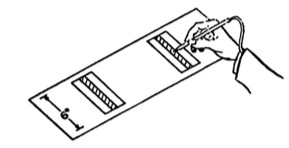
\includegraphics[width=\textwidth]{images/illustrations/fitt_ex1}
		\captionof{figure}{Illustration af Fitts' første eksperiment, med pegeredskab og seks lodrette plader \cite{fitts1954}}
		\label{fig:FittsEx1}
	\end{minipage}
	\begin{minipage}[b]{.1\linewidth}
		~
	\end{minipage}
	\begin{minipage}[b]{.45\linewidth}
		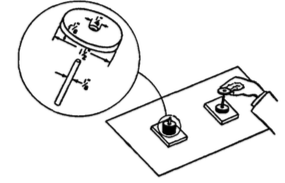
\includegraphics[width=\textwidth]{images/illustrations/fitt_ex2}
		\captionof{figure}{Illustration af Fitts' andet eksperiment med to pinde og otte runde plader \cite{fitts1954}}
		\label{fig:FittsEx2}
	\end{minipage}
\end{minipage}

\addcontentsline{toc}{subsection}{Eksperiment 3}
\subsection*{Eksperiment 3: \textit{Pin Transfer}}
Udførelsen af dette eksperiment krævede et sæt af otte pinde og 16 huller, delt i to sæt. Diameteren på de otte pinde kunne antage fire forskellige størrelser, alt imens afstanden imellem de to sæt huller kunne være af fem forskellige længder. Opstillingen kan ses af figur \ref{fig:FittsEx3}.
Hver af de 20 mulige forsøgsopstillinger blev udført i tilfældig rækkefølge af 20 mandlige universitetsstuderende.
\begin{figure}[h]
\centering
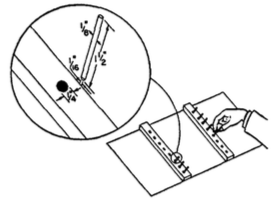
\includegraphics[width=0.5\linewidth]{images/illustrations/fitt_ex3}
\captionof{figure}{Illustration af Fitts' tredje eksperiment med 8 pinde og 16 huller \cite{fitts1954}}
\label{fig:FittsEx3}
\end{figure}

\addcontentsline{toc}{subsection}{Fitts' konklusion}
\subsection*{Fitts' konklusion}
Resultaterne som Fitts fik fra de udførte eksperimenter viste, at des større afstand målene imellem, desto længere tid brugte testdeltagerne. For at bevise sin teori udledte Fitts et \textit{Index of Difficulty}, $ID$, som beskriver sværhedsgraden af en given motorisk opgave på baggrund af størrelsen, $W$, og på afstanden, $A$, til målet.
\begin{align*}
ID = -\log_2\left(\frac{W}{2A}\right)
\end{align*}
Brugen af $\log_2$ i formlen, er baseret på Fitts' kendskab til Shannon's sætning 17 \cite{goldberg2015}. For at sikre at $ID$ altid giver en positiv værdi, valgte Fitts at gøre brug af $2A$ frem for $A$, da det kan garanteres at $2A > W$, hvilket sikrer det samme fortegn for alle udfald af logaritmen. Da $log\left(\frac{W}{2A}\right)<0$, for $0<\frac{W}{2A}<1$, valgte Fitts at multiplicere det med $-1$, hvilket sikrer at ID altid er positiv.
Ved brug af $ID$ udregnede Fitts et \textit{Index of Performance}, IP, som beskriver hvorledes en opgave er udført i forhold til sværhedsgraden, $ID$, og tiden $t$.
\begin{align*}
IP &= \frac{ID}{t}\Leftrightarrow\\
IP &= \frac{-1}{t}\log_2\left(\frac{W}{2A}\right)
\end{align*}
Denne formel er dog ikke den klassiske formel for Fitts lov, men ved omregninger kan den findes. Vi ser først på ID.
\begin{align*}
ID &= -\log_2\left(\frac{W}{2A}\right) \Leftrightarrow\\
ID &= -\log_2\left(W\right)-\left(-\log_2\left(2A\right)\right) \Leftrightarrow\\
ID &= \log_2\left(2A\right)-\log_2\left(W\right) \Leftrightarrow\\
ID &= log_2\left(\frac{2A}{W}\right)
\end{align*}
Vi kan indsætte dette i formlen for IP, og isolere et udtryk for tiden $t$.
\begin{align*}
IP &=\frac{-1}{t}\log_2\left(\frac{W}{2A}\right) \Leftrightarrow\\ 
IP &= \frac{1}{t}\log_2\left(\frac{2A}{W}\right) \Leftrightarrow\\ 
t &= \frac{\log_2\left(\frac{2A}{W}\right)}{IP}
\end{align*}
Da det virker uoverskueligt i sådan en formel at dividere med IP, så substitueres denne værdi med $IP = \frac{1}{b}$, hvilket giver anledning til en formel som er nemmere at bruge, og forstå.
\begin{align*}
t &= \frac{\log_2\left(\frac{2A}{W}\right)}{\frac{1}{b}} \Leftrightarrow\\ 
t &= b \cdot \log_2\left(\frac{2A}{W}\right)
\end{align*}
Når man regner med det menneskelige motoriske system, så skal der medregnes den tid det tager for et menneske at opfatte at en opgave er startet. Fitts fandt frem til dette led, $a$, ved at benytte lineær regression på sine data.
\begin{equation}
\label{eq:FittsLov}
T = a + b \cdot log_2\left(\frac{2A}{W}\right)
\end{equation}
Dette er hvad der i dag kendes som Fitts lov.

Crossman og Goodeve \cite{crossman1983} forklarer Fitts lov som en overordnet bevægelse fra startpositionen i mod målet, hvorefter der ved én eller flere underbevægelser korrigeres for den fejl der blev foretaget ved den overordnede bevægelse. En illustration af bevægelsens hastighed over afstanden er vist i figur \ref{fig:CrossmanFitt} med en serie af tre delbevægelser, hvoraf den overordnede bevægelse begynder i startpositionen med afstand 0.
\begin{figure}[h]
\centering
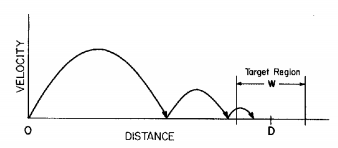
\includegraphics[width=.5\linewidth]{images/illustrations/base_model_fitt}
\caption{Illustration af hastighed over distance, der viser hoved- og underbevægelser brugt af Crossman og Goodeve til at forklare Fitt's lov \cite{meyer1988}}
\label{fig:CrossmanFitt}
\end{figure}

\newpage
\addcontentsline{toc}{section}{Alternative formuleringer}
\section*{Alternative formuleringer}
Siden udgivelsen af Fitts’ artikel, har flere forskere forsøgt at finde en formel, der passer bedre på det motoriske system, end Fitts’ originale lov. Der har indenfor menneske-datamaskine interaktion været flere udgivelser, som mener at have fundet en mere præcis formel end Fitts’ lov, eller som kigger på andre former for eksperimenter. Vi vil i dette afsnit se nærmere på tre af sådanne formuleringer.

\addcontentsline{toc}{subsection}{Welfords formulering}
\subsection*{Welfords formulering}

I \cite{welford1968} beskriver Welford en række fundamentale forudsætninger for det menneskelige motoriske system. Her kiggede han blandt andet på Fitts' lov, og de data han indsamlede i sit første forsøg. Han mente at Fitts' lov i princippet gengav den indsamlede data præcist, men han så også tre utilfredsstillende egenskaber, hvilket fik ham til at foreslå følgende modifikationer.
\begin{figure}[h]
\centering
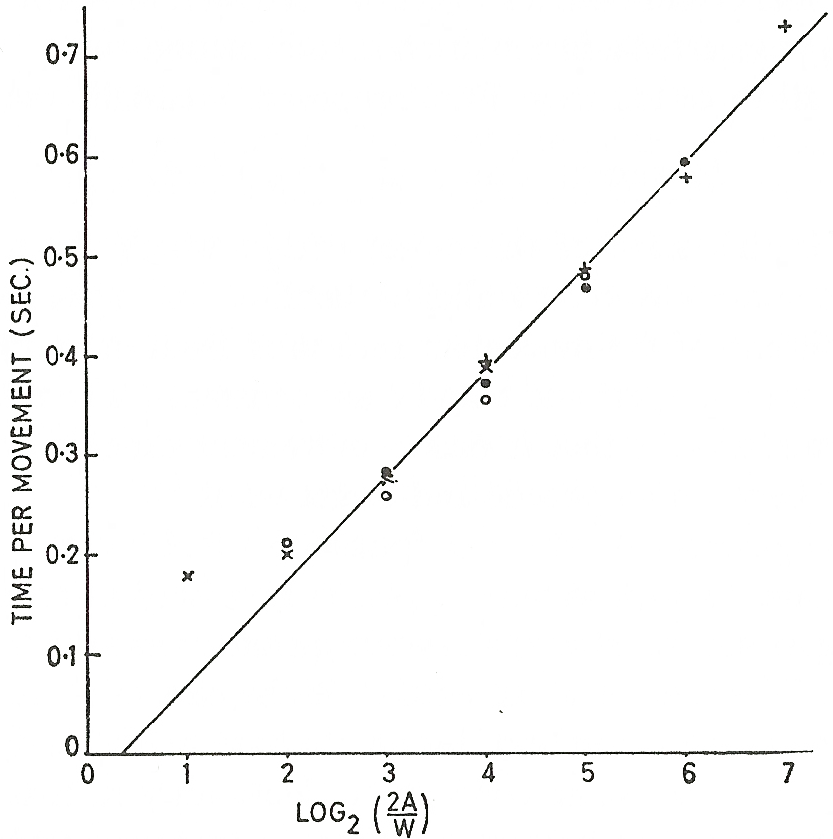
\includegraphics[width=.5\linewidth]{images/illustrations/welford_plot_1}
\caption{Graf over $MT$ (y-akse) I forhold til $ID$ (x-akse), med punktplot over data fra et af Fitts' forsøg, og linje der viser hvordan Fitts' model passer på dataen.}
\label{fig:WelfordGraf}
\end{figure}
Welford argumenterede for, at der skulle undlades at multiplicere $A$ med $2$, da det på data fra Fitts' første forsøg, ville resultere i en negativ $a$-værdi. Derved bliver Ligning \ref{eq:FittsLov} til
\begin{align}
\label{eq:Crossman}
T = a + b \cdot log\left(\frac{A}{W}\right)
\end{align}
som også tidligere var blevet udledt af Crossman \cite{crossman1957}. Hvis data fra Fitts' første forsøg indsættes i Ligning \ref{eq:Crossman}, så vil $a$ ligge tæt på $0.05$. Dette passer med Crossman's eksperiment, hvor tiden man bruger, inden bevægelsen begynder, udregnes til at være cirka $0.05$ \cite{crossman1957}. Welford argumenterer for, at man derved helt kunne undlade $a$, da det beskriver tiden inden bevægelsen. I et lignende eksperiment \cite{welford1958} fandt man dog, at resultaterne generelt var mere troværdige, hvis $a$-leddet var medtaget.

Figur \ref{fig:WelfordGraf} viser data fra ét af Fitts' eksperimenter og den tilhørende affine kurve. Den affine kurves skæring med $y$-aksen rammer under nul, jvf. den negative $a$ værdi. På baggrund af de to første punkter, som ikke ligger på den affine linje, fandt Welford frem til, at følgende modifikationer til ligning \ref{eq:FittsLov} ville beskrive data punkterne bedre.
\begin{align}\label{eq:WelfordsLov}
T = K \cdot log\left(\frac{A + \frac{1}{2}W}{W}\right) = K \cdot log\left(\frac{A}{W} + 0.5\right)
\end{align}
Ligning \ref{eq:WelfordsLov} er sidenhen blevet kendt som Welfords lov og har betydning for hvordan tiden, $T$, opfattes. Tiden vil i Ligning \ref{eq:WelfordsLov} blive afhænging af en Weber Fraction \cite{welford1958}, da testpersonen skal skelne mellem længderne til målets fjerneste og næreste kant. Testpersonen skal altså udvælge en længde, $W$, ud fra den totale længde mellem startpunktet og målets fjerneste kant. Det er her vigtigt at notere at Ligning \ref{eq:WelfordsLov} også opretholder den fordel, som Fitts hævdede der var ved at multiplicere $A$ med $2$. Dette ses ud fra det mest ekstreme tilfælde, hvor bevægelsens startpunkt er på målets kant, da $A = \frac{1}{2}W$ vil gælde, hvorved $T = K \cdot log\left(\frac{A + \frac{1}{2}W}{W}\right) = K \cdot log\left(\frac{W}{W}\right)$. Da $W > 0$ vil $log(W) > 0$.

Den sidste observation, der blev gjort, var at kurven i figur~\ref{fig:WelfordGraf} viser en tydelig udfladning ved lavere værdier af $x$. Welford noterede at det sandsynligvis var grundet en begrænsende faktor som beskriver en minimumstid per bevægelse, hvor kort eller uhindret bevægelse end måtte være. Welford's egne undersøgelser har påvist at denne begrænsende faktor har betydning for hvor meget af målet der rent faktisk bliver brugt. Når målene er brede og længden mellem dem kort, så vil testpersonen kun bruge en sub-længde af målets fulde længde. Han overfører mere information end Ligning \ref{eq:WelfordsLov} ville beskrive, fordi den effektive W er kortere. Den kortere bredde kan i nogen omfang afspejles i en reduktion af fejl og, hvis reduktionen sker med behørigt hensyn, så holder Ligning \ref{eq:WelfordsLov} stadig.

Ud fra de tre ovenstående modifikationer indførte Welford igen Fitts' data fra hans første forsøg i et koordinatsystem. Denne gang havde dataen dog været igennem fejlreduktion og blev indsat op imod Welford's formulering, hvilket viste at Ligning \ref{eq:WelfordsLov} var bedre til at beskrive dataen end Ligning \ref{eq:FittsLov}. Den affine kurve som Welford kom frem til er at se i figur \ref{fig:WelfordGraf2}
\begin{figure}[h]
\centering
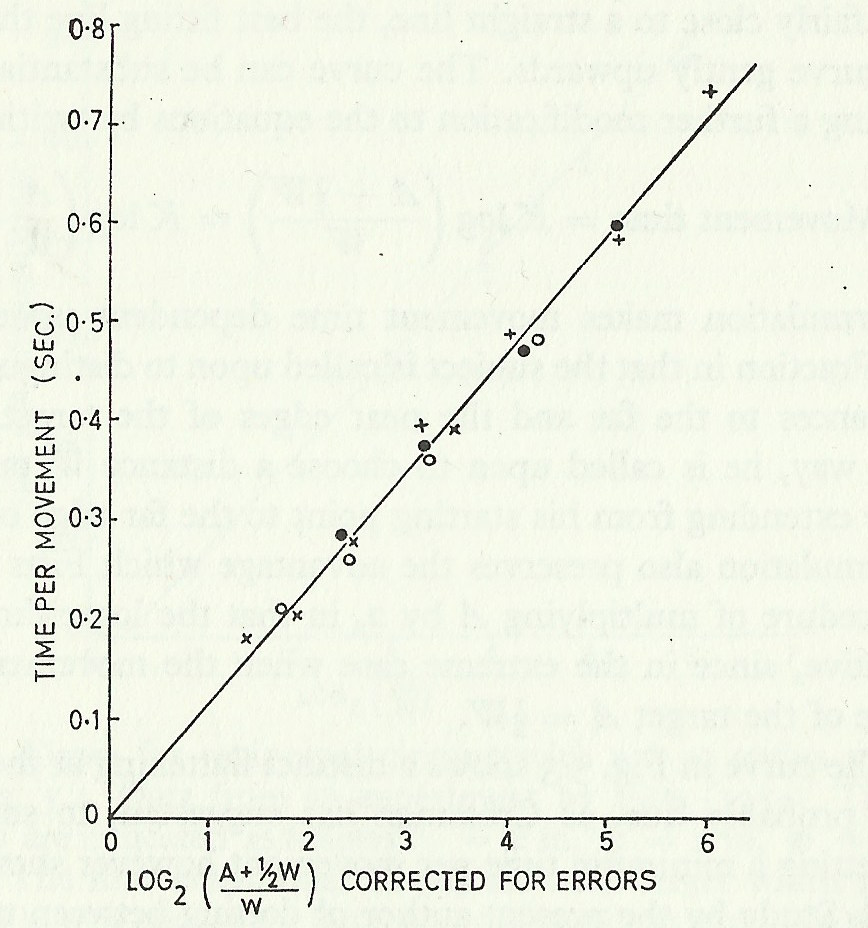
\includegraphics[width=.5\linewidth]{images/illustrations/welford_plot_2}
\caption{Graf over $MT$ (y-akse) I forhold til $ID$ (x-akse), med punktplot over data fra et af Fitts' forsøg, og linje der viser hvordan Welfords model passer på dataen.}
\label{fig:WelfordGraf2}
\end{figure}

\addcontentsline{toc}{subsection}{MacKenzies formulering}
\subsection*{MacKenzies formulering}
MacKenzie udgav i 1992 en artikel~\cite{mackenzie1992}, hvor han ser nærmere på Fitts' Lov og seks alternative studier af samme. Han gennemgår en række forbedringer af den originale model, og fremstiller en alternativ formulering til $ID$, som han beskriver som værende mere teoretisk forsvarlig, nemlig:
\begin{align}
T=a+b\cdot\log_2\left({\frac{A+W}{W}}\right)
\end{align}

Han nævner i afsnittet \emph{Physical Interpretation} at skæringspunktet ideelt set vil ligge i nul, hvilket tyder på, at en opgave med $ID=0$ vil tage 0 sekunder. Ifølge MacKenzie modvises dette normalt ved lineær regression på forsøgsdata, som ofte medfører et skæringspunkt, der ikke ligger i nul. Dette bruger han som argument for, at der findes en additiv faktor som er urelateret til ID.\\

En af de mest accepterede udledninger af Fitts' lov stammer fra modellen \emph{deterministic error-corrections} originalt fremstillet af \cite{crossman1983}, og bygger på idéen om at en bevægelsesopgave består af en række iterative korrigerende bevægelser. MacKenzie refererer til simpliciteten af denne model som værende appellerende, men kalder de underliggende antagelser for suspekte. Han refererer til \cite{langolf1976}, hvor der blev observeret bevægelsesopgaver som kun indeholdte én korrigerende bevægelse, selvom det generelt forudses at der vil være flere korrigerende bevægelser ved en vis størrelse af $A/W$.\\

\begin{figure}[h]
\centering
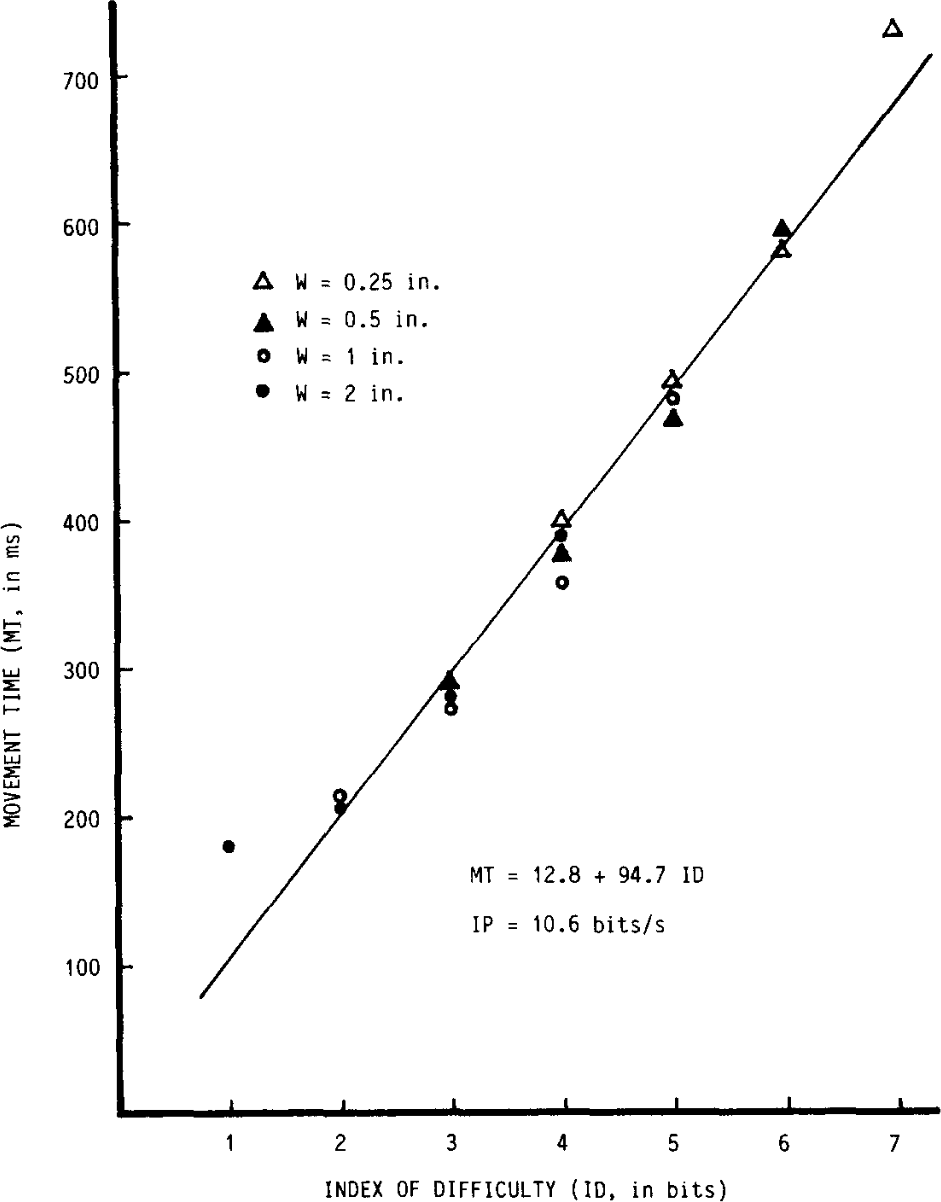
\includegraphics[width=.5\linewidth]{images/illustrations/mackenzie_plot_1}
\caption{Graf over $MT$ (y-akse) I forhold til $ID$ (x-akse), med punktplot over data ved forskellige værdier af $W$, og linje der viser hvordan Fitts' model passer på dataen.}
\label{fig:MacKenziePlot1}
\end{figure}
MacKenzie beskriver, at et af problemerne med Fitts' Lov er den tætte relation mellem $ID$ og $MT$. Figur~\ref{fig:MacKenziePlot1} illustrerer, hvordan punkterne flader ud, ved lave værdier af $ID$, mens kurven beholder sit $1:1$-forhold mellem $ID$ og $MT$. Der er altså en usammenhæng mellem de observerede og forudsagte værdier, hvilket også er blevet observeret i flere andre studier som \cite{welford1960, buck1986, crossman1983, drury1975, klapp1975, langolf1976, meyer1988, wallace1978}\\
Han fremhæver dog, at der er lavet en del studier af Fitts' lov og, at der er blevet præsenteret en del alternative formuleringer, som forsøger at få de faktiske data til at passe bedre til modellen. Specielt fremhæver han Welford's~\cite{welford1960,welford1968}, da den er udbredt som alternativ til Fitts' originale formulering. MacKenzie nævner den ekstreme lighed mellem Welford og Shannons formulering, og beskriver hvordan det for nyligt er blevet vist at Paul Fitts originale formulerings forhold mellem $A$ og $W$ havde baggrund i en approksimation af Shannon's sætning~\cite[p. 388]{fitts1954}, som var blevet introduceret med en advarsel om at brugbarheden kun gjaldt ved et højt signal-til-støj forhold. Dette giver selvfølgelig problemer når der i Fitts' originale forsøg bliver brugt et forhold helt ned til 1:1 mellem A og W. MacKenzie foreslår at man benytter sig af en form der minder meget om Welford's, men her er en direkte analogi til Shannon's formulering:
\begin{align}
\text{Shannon: }C=B\times&\log{\frac{S+N}{N}}\\
\text{Welford: }MT=a+b\times&\log{\frac{A+0.5W}{W}}\\
\text{MacKenzie: }MT=a+b\times&\log{\frac{A+W}{W}}
\end{align}

Forskellen mellem Fitts' originale formulering for $ID$, og MacKenzie's bud på en ny formulering lavet som en direkte analogi til Shannon's bliver sammenlignet i figur~\ref{fig:MacKenziePlot2}, hvor det er tydeligt, at der ved lavere værdier af $A$ sker en udfladning af kurven, hvilket passer med data punkterne i figur~\ref{fig:MacKenziePlot1}, jvf. det første data punkt som ikke ligger på den affine linje.\\
\begin{figure}[h]
\centering
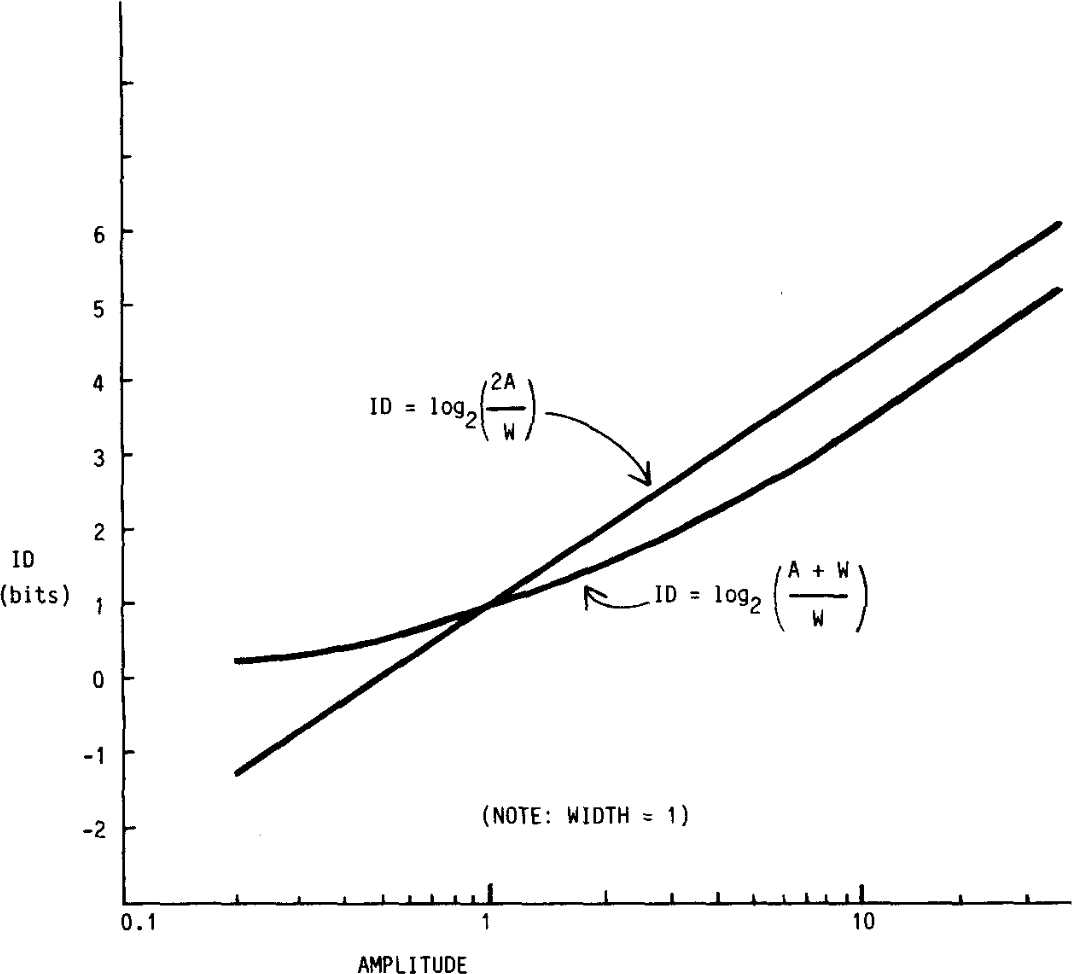
\includegraphics[width=.5\linewidth]{images/illustrations/mackenzie_plot_2}
\caption{Graf over $ID$ (y-akse) I forhold til $A$ (x-akse), med to linjer der viser en sammenligning af Fitts' og MacKenzies model ved fastholdt værdi af $W$.}
\label{fig:MacKenziePlot2}
\end{figure}
MacKenzie ser hans formulering som værende en mindre forbedring i forhold til Welford's, og mener ikke at man vil kunne se den store forskel mellem Welfords og sin formulering, medmindre man har at gøre med $ID$ som er under 3 bits. Han kommer frem til de 3 bits ved at se på figur~\ref{fig:MacKenziePlot2}, hvor det ses, at de to formuleringer for $ID$ er parallelle med hinanden, indtil omkring 3 bits eller derunder.\\

Det generelle problem med MacKenzie's artikel er at han ikke kommer med noget teoretisk grundlag for hans formulering, og derved ikke kan forklare hvorfor hans formulering er mere præcis end andre, eller hvorfor det netop er bedre med en direkte analogi til Shannon's i forhold til Welford's. I artiklen~\cite{drewes2010} bliver der stillet spørgsmålstegn ved dette. Men hvis man ser bort fra det manglende teoretiske grundlag, så er MacKenzies formulering stadig en af de mest udbredte og brugte varianter af Fitt's lov, og har vist sig at passe godt på udførte forsøg~\cite{goldberg2015}.

\addcontentsline{toc}{subsection}{Meyers formulering}
\subsection*{Meyers formulering}
\begin{figure}[h]
\centering
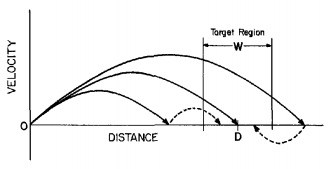
\includegraphics[width=.5\linewidth]{images/illustrations/base_model_meyer}
\caption{Stochastic optimized-submovement modellen - Den horisontale akse repræsenterer afstand og den vertikale akse repræsenterer bevægelseshastighed. De faste linjer repræsentere primære underbevægelser, mens stiplede linjer er korrigerende underbevægelser. Bevægelserne tager udgangspunkt i en startende position (afstand = 0) og skal bevæge sig til et mål, med center i D og bredde W.}
\label{fig:MeyerTheory}
\end{figure}
Som beskrevet i forrige afsnit, så basere Fitts' lov sig på \emph{deterministic error-corrections} modellen. Meyer et. al foreslog en ny model, kaldet stochastic optimized-submovement modellen, som de baserede deres formel på \cite{meyer1988}. Som det ses af Figur \ref{fig:MeyerTheory} så basere denne model sig på at personer laver en primær underbevægelse og derefter, hvis der er behov for det, en korrigerende underbevægelse. Udfra denne model kan den gennemsnitlige tid, $T$, forudsiges til at være
\begin{equation}
\label{eq:meyer}
T = a + b \sqrt{\frac{A}{W}}
\end{equation}

Meyer et. al udfører et teoretisk og to praktiske forsøg, hvor der i det teoretiske forsøg bliver gjort flere udregninger med forskellige værdier af A og W, som viser en god approksimation i forhold til Fitts' formulering. De praktiske forsøg gør brug af simplere motoriske opgaver end dem kendt fra Fitts' egne forsøg. Den eneste rummelige frihed i Meyers forsøg er håndledenes rotation. Igennem hele artiklen benytter Meyer sig af, at en motorisk opgave er delt ind i en primær underbevægelse, og nogle efterfølgende korrigerende underbevægelser. Dette har dog ikke nogen betydning for sammenligningen med Fitts’ formulering, da den totale tid af alle underbevægelser vil approksimere den logaritmiske funktion af A/W, hvilket medfører at Fitts model også passer på modeller med iterative fejlkorrigerende underbevægelser.

Graferne for funktionerne i ligning \ref{eq:meyer} og \ref{eq:FittsLov} vil udvise samme form. Grunden til dette er begge funktioner monotont voksende, når $\frac{A}{W}$ bliver større, $\sqrt{\frac{A}{W}}$ vokser dog hurtigere end den tilsvarende logaritmiske funktion, hvilket kan ses af figur \ref{fig:log_vs_sqrt}. 

\cite{goldberg2015} noterer dog, at der er nogle ulemper ved denne formel. Hvis testdeltageren når målet i en enkelt bevægelse, så vil modellen følge en lineær udvikling i stedet for en eksponentiel udvikling. Dette passer ikke godt med observerede værdier. For en fast positiv værdi af $\frac{A}{W}$ vil Meyers formel gå mod $1$, når antallet af underbevægelser går mod uendelig.

\begin{figure}[h]
\centering
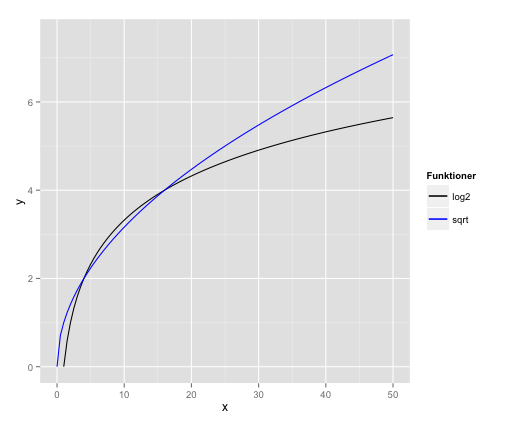
\includegraphics[width=.7\linewidth]{images/illustrations/meyer_plot_comparison}
\caption{Graf over $x$ og $y$ ved et fastdefineret interval, der illustrerer udviklingen af funktionerne $y=log2(x)$ og $y=sqrt(x)$.}
\label{fig:log_vs_sqrt}
\end{figure}

\addcontentsline{toc}{section}{Sammenligning}
\section*{Sammenligning}
For at få en bedre forståelse af de fire formuleringer af Fitts' lov, vil vi i dette afsnit se på hvordan de matematisk ligner hinanden. Det første vi vil gøre er at prøve at omformulere Welford's formulering, da den ikke indeholder et additivt `a'-led. 
\begin{align*}
T &= K\cdot\log\left(\frac{A+0.5W}{W}\right)\Leftrightarrow\\
T &= K\left(1-1+\log\left(\frac{A+0.5W}{W}\right)\right)\Leftrightarrow\\
T &= -K+K\left(1+\log\left(\frac{A+0.5W}{W}\right)\right)\Leftrightarrow\\
T &= -K+K\left(\log(2)+\log\left(\frac{A+0.5W}{W}\right)\right)\Leftrightarrow\\
T &= -K+K\left(\log\left(2\left(\cdot\frac{A+0.5W}{W}\right)\right)\right)\Leftrightarrow\\
T &= -K+K\cdot\log\left(\frac{2A+W}{W}\right)
\end{align*}
På trods af at det er muligt at omformulere Welford's formulering, så vil det ikke være brugbart i praksis. Omformuleringen gør, at det additive led, $a = -K$, er blevet negativt, hvilket betyder at tiden det tager at påbegynde en opgave er negativ. Vi vil derfor fremadrettet kun bruge Welford's formulering uden den additive konstant.

Når vi kigger på de fire formuleringer, så kan vi vise, at de ikke er ens, ved at vælge et fast $A = 5$ og $W = 1$ og finde ét punkt, hvor de to funktionsværdier er forskellige. Vi sætter $a=0$ og finder tiden i skæringen med $y$-aksen.
\begin{align*}
\text{Fitts: } &T=b\cdot\log\left(\frac{2\cdot5}{2}\right)\\
\text{Welford: } &T=k\cdot\log\left(\frac{5+0.5\cdot 2}{2}\right)\\
\text{Mackenzie: } &T=b\cdot\log\left(\frac{5 + 2}{2}\right)\\
\text{Meyer: } &T=b\cdot\sqrt{\frac{5}{2}}
\end{align*}
Ved at sætte to af ligninerne for $T$ lig hinanden kan vi vise, at de to formuleringer ikke er ens.
\begin{align*}
b_{Fit}\cdot\log\left(\frac{2\cdot5}{2}\right)&=b_{Mac}\cdot\log\left(\frac{5 + 2}{2}\right)\\
b_{Mac} &= \frac{b_{Fit}\cdot\log\left(\frac{2\cdot5}{2}\right)}{\log\left(\frac{5 + 2}{2}\right)}
\end{align*}
Indsætter vi denne værdi for $b_{Mac}$ i Mackenzies formulering, kan vi finde frem til, at Mackenzies og Fitts formuleringer kun er ens, såfremt $ID$ ledet er ens, hvilket ikke er tilfældet.
\begin{align*}
\text{Mackenzie: } &T =\frac{b_{Fit}\cdot\log\left(\frac{2\cdot5}{2}\right)}{\log\left(\frac{5 + 2}{2}\right)}\cdot\log\left(\frac{5 + 2}{2}\right)\\
\text{Mackenzie: } &T =b_{Fit}\cdot\log\left(\frac{2\cdot5}{2}\right)
\end{align*}

Denne sammenligning af formuleringerne to og to kan gøres for dem alle fire, men det vil vi undlade at gøre her, og blot formode, at det rent faktisk er tilfældet for dem alle sammen. De fire formuleringer er derfor ikke ens og vi vil derfor få forskellige resultater når vi bruger dem på den indsamlede data.

På trods af at de fire formuleringer er forskellige, så vil de kunne approksimere hinanden. Vi har derfor plottet de fire formulering i ét interval, for at se om de approksimere hinanden. Figur \ref{fig:Sammenligning} viser $ID$ som funktion af $A/W$ og viser at Meyer's, Welford's og MacKenzie's approksimere hinanden for $A/W$-værdier mellem 0 og 25. Grafen for Fitts' ligger højere end de tre andre og approksimere ikke de andre.

\begin{figure}[h]
\centering
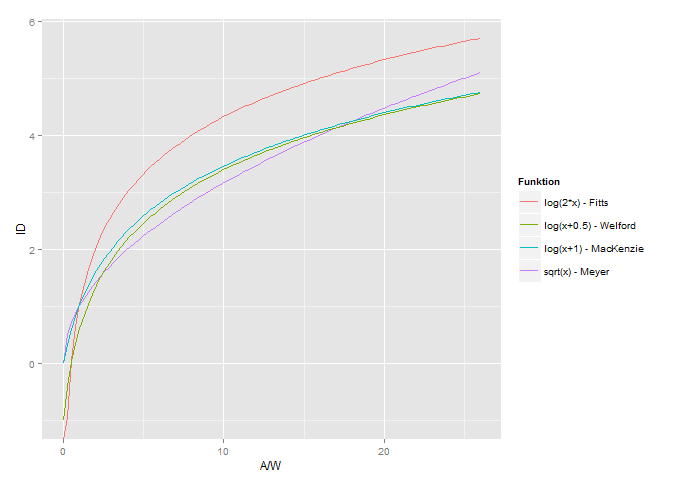
\includegraphics[width=\linewidth]{images/plots/plot_comparison_id}
\caption{Graf over $ID$ (y-akse) I forhold til $A/W$ (x-akse) med linjer der viser udviklingen af $ID$-funktionen for de fire forskellige modeller.}
\label{fig:Sammenligning}
\end{figure}

\addcontentsline{toc}{chapter}{Design}
\chapter*{Design}
I dette afsnit beskriver vi det design der er brugt i vores forsøg. Derudover vil vi også beskrive vores forsøgsopstillinger.

\addcontentsline{toc}{section}{Forsøgsopstilling}
\section*{Forsøgsopstilling}
Vi har valgt at udføre to brugerundersøgelser, for at have både et kontrolleret og et ukontrolleret datasæt med deltagernes bevægelsesbaner.
Det første vil være et kontrolleret laboratorieeksperiment hvor vi kontrollerer flest mulige variable, mens det andet er et ukontrolleret crowdsourcing- og webbaseret eksperiment hvor vi får en større mængde data, men ikke har den samme kontrol over eksperimentets variable.\\\\
Større dele af vores eksperiment har vi valgt at udføre ligesom tidligere udførte forsøg, da de er udført at folk med meget mere erfaring, og ekspertise på dette område end os.
Det drejer sig om følgende dele af vores eksperiment:
\begin{itemize}
\item Spørgsmål som blev stillet før crowdsourcing-deltagerne kunne udføre forsøget \cite{goldberg2015}
\item Design af pegeopgave, inklusiv værdier af A, W og canvas \cite{goldberg2015}
\item Størrelser af A og W til tunnelopgave \cite{accot1997}
\item Antal vindinger af spiral til spiralopgave \cite{accot1997}
\end{itemize}
Derudover har vi brugt samme udformning af tunnel- og spiralopgave, som i pegeopgaven. Det vil sige, at vi har samme farver til mål, og samme design af testfladen.

\addcontentsline{toc}{section}{Platform og udviklingsværktøj}
\section*{Platform og udviklingsværktøj}
Vi har valgt at bruge JavaScript til at udvikle vores forsøg, da vi alle er bekendte med sproget, så vi skal ikke til at sætte os ind i noget nyt. Derudover er det integreret i alle browsere nu om dage, hvilket gør det nemt at crowdsource. For at generere vores opgaver har vi valgt at gøre brug af JavaScript-frameworket $paper.js$. Det gør brug af HTML5 canvas og er bagudkompatibelt til IE9. Frameworket gør det muligt at autogenerere cirkler til vores pegeopgaver, gemme bevægelsesbaner og tegne tunneller, til tunnelopgaverne.

\addcontentsline{toc}{section}{Opgavetyper}
\section*{Opgavetyper}
I denne sektion vil vi beskrive hvordan tunnel-, spiral- og pegeopgaverne er designet.

\addcontentsline{toc}{subsection}{Tunnelopgave}
\subsection*{Tunnelopgave}
\begin{minipage}{\linewidth}
	\begin{minipage}{\textwidth}
		\centering
		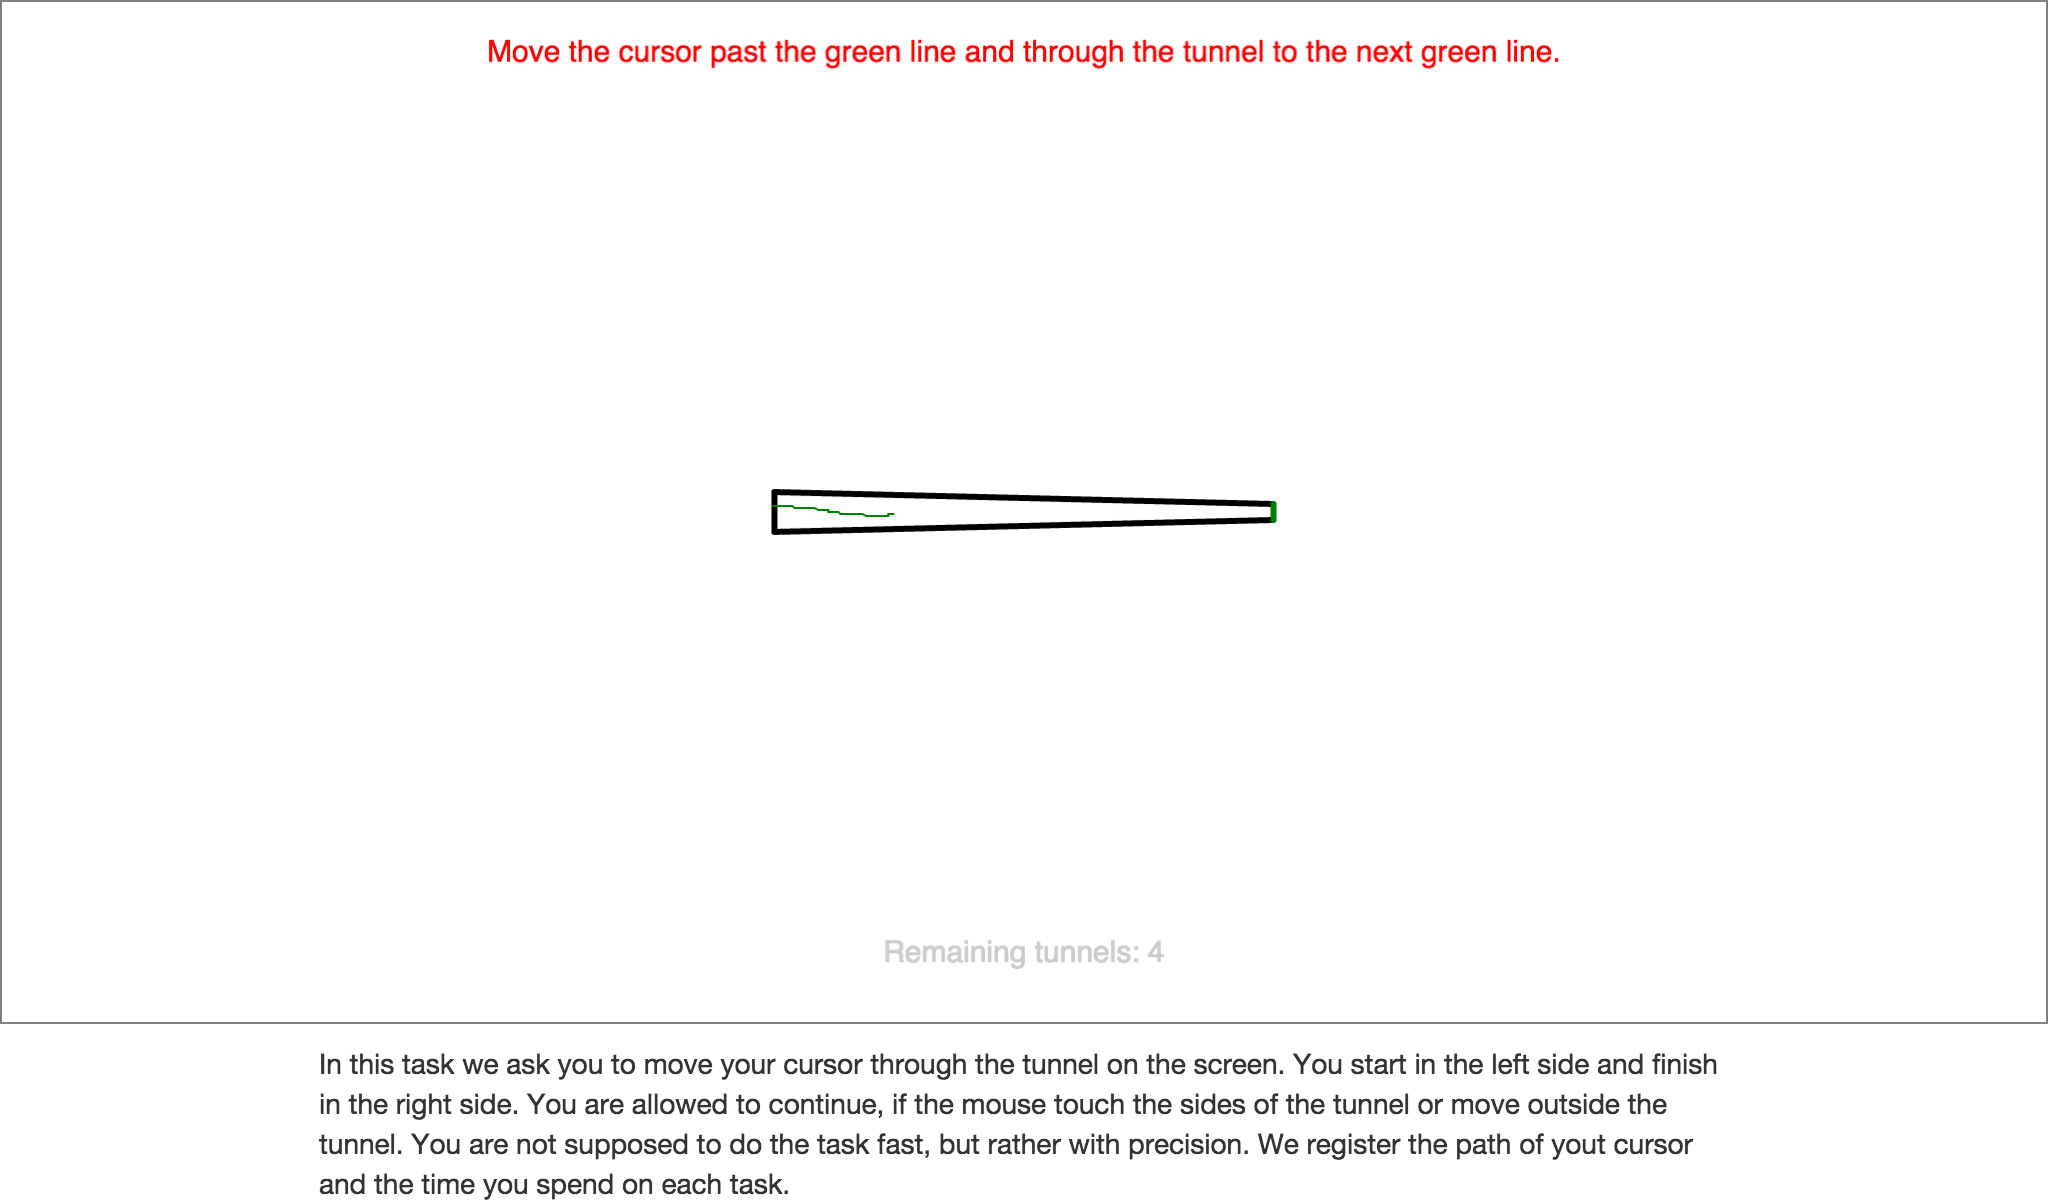
\includegraphics[width=\textwidth, trim = .5cm 20cm .5cm 15cm, clip]{images/screenshots/ex_step_4_tunnel_path}
		\captionof{figure}{Skærmbillede af den første tunnelopgave, med starten af en testpersons sti.}
		\label{fig:ex_tunnel_1}
	\end{minipage}
	\begin{minipage}{\textwidth}
		\centering
		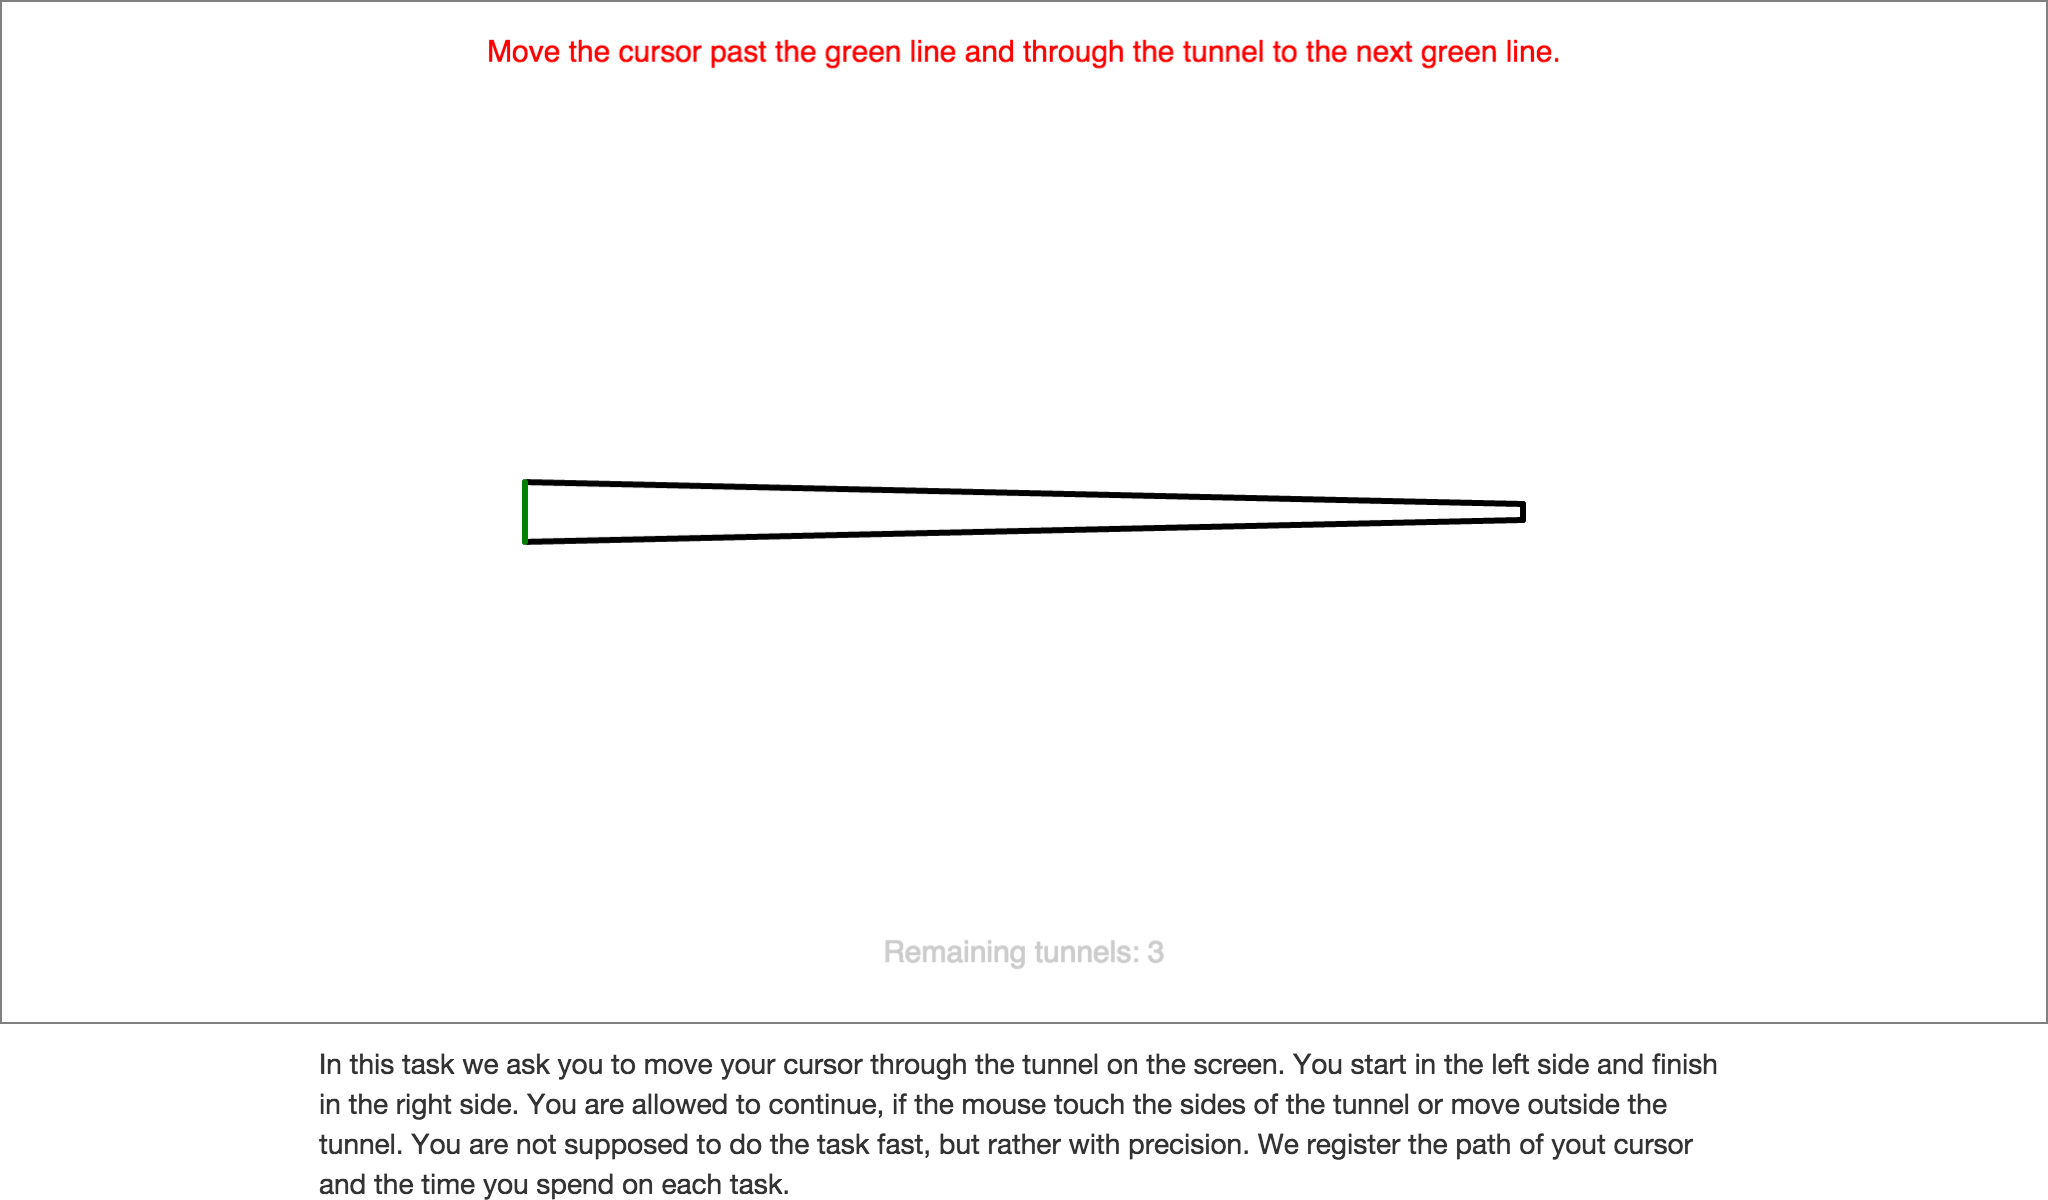
\includegraphics[width=\textwidth, trim = .5cm 20cm .5cm 15cm, clip]{images/screenshots/ex_step_4_tunnel_2}
		\captionof{figure}{skærmbillede af den anden tunnelopgave.}
		\label{fig:ex_tunnel_2}
	\end{minipage}
	\begin{minipage}{\textwidth}
		\centering
		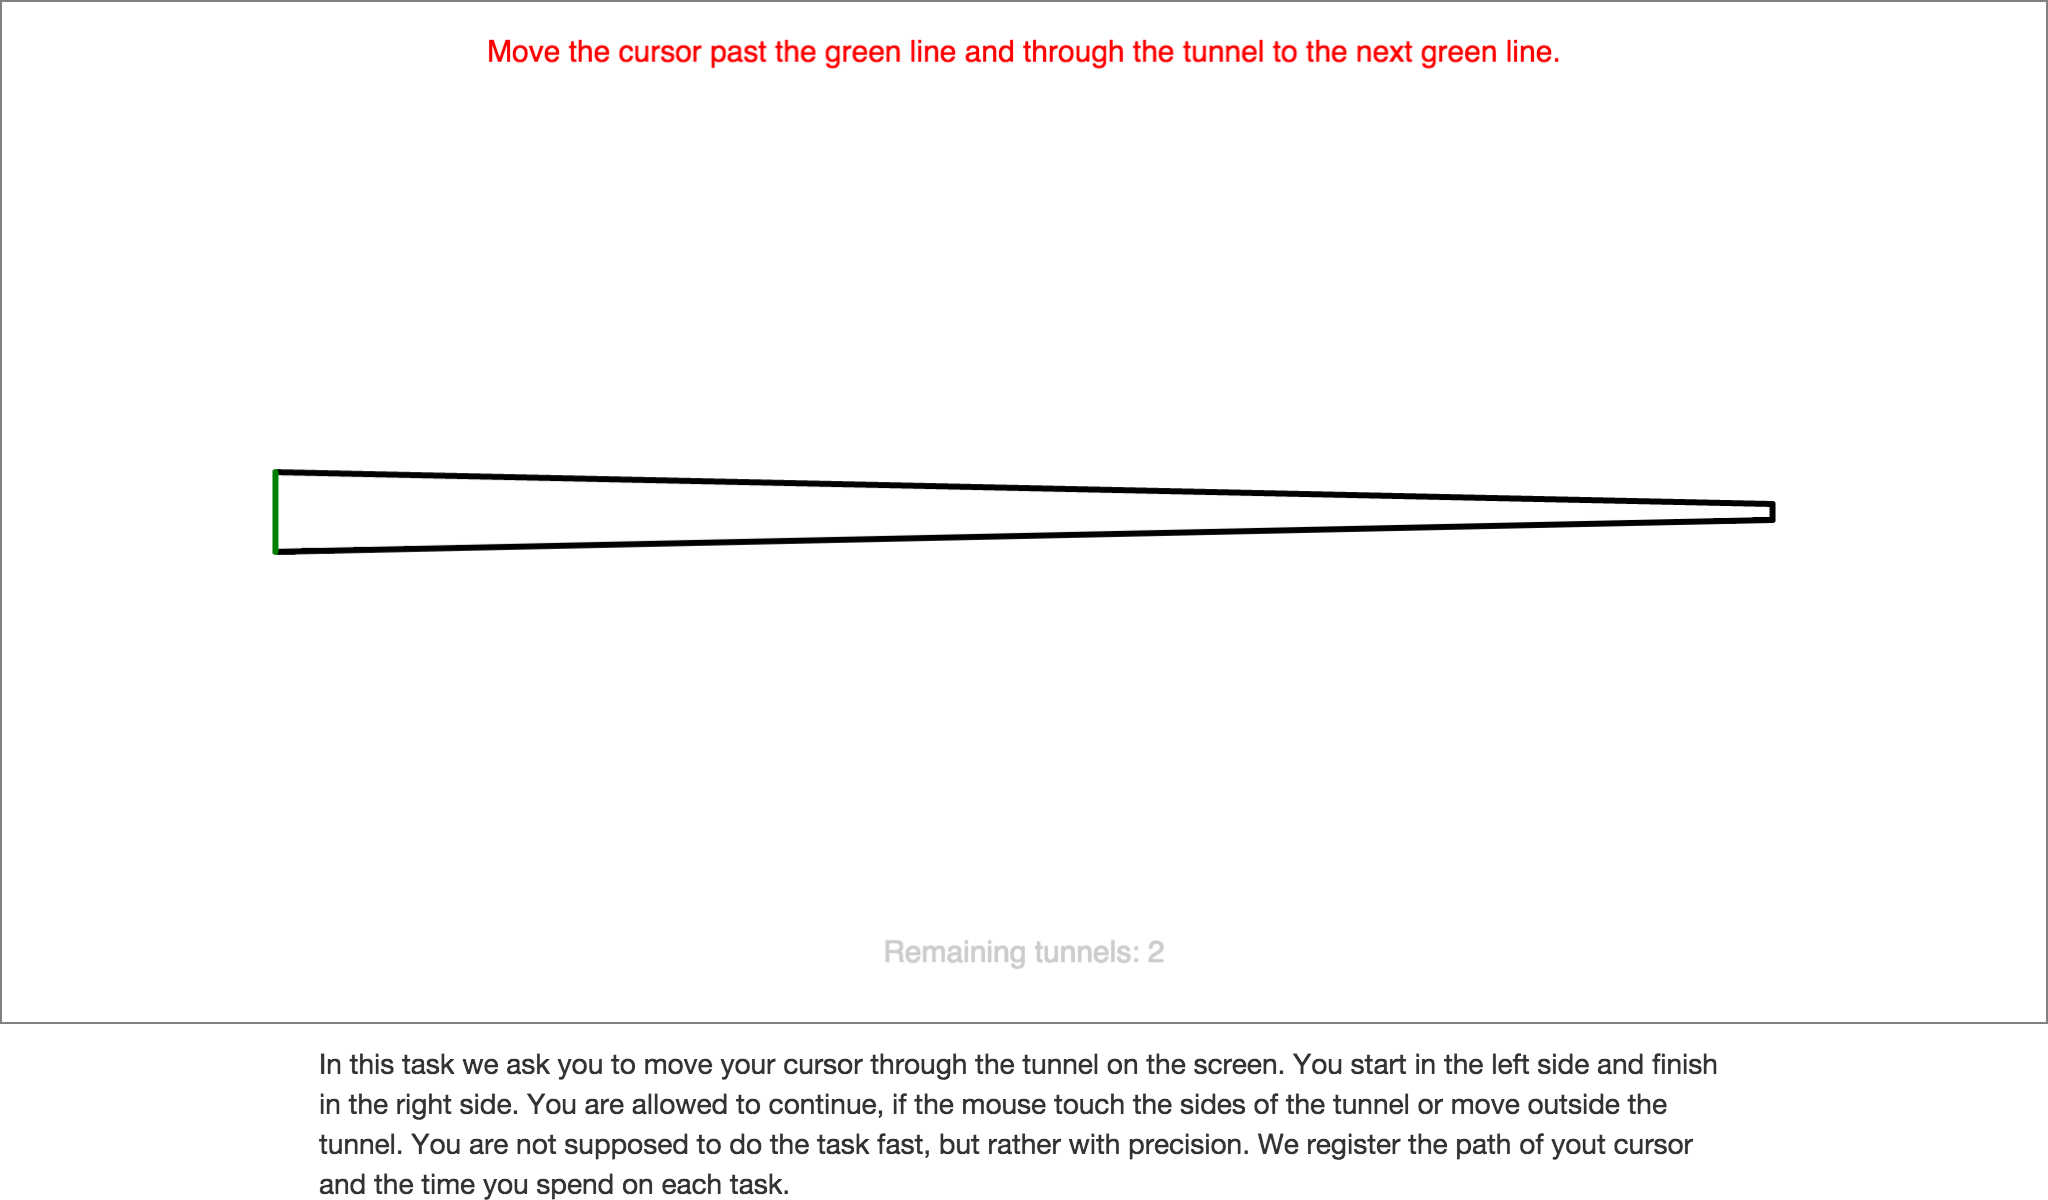
\includegraphics[width=\textwidth, trim = .5cm 20cm .5cm 15cm, clip]{images/screenshots/ex_step_4_tunnel_3}
		\captionof{figure}{Skærmbillede af den tredje tunnelopgave.}
		\label{fig:ex_tunnel_3}
	\end{minipage}
	\begin{minipage}{\textwidth}
		\centering
		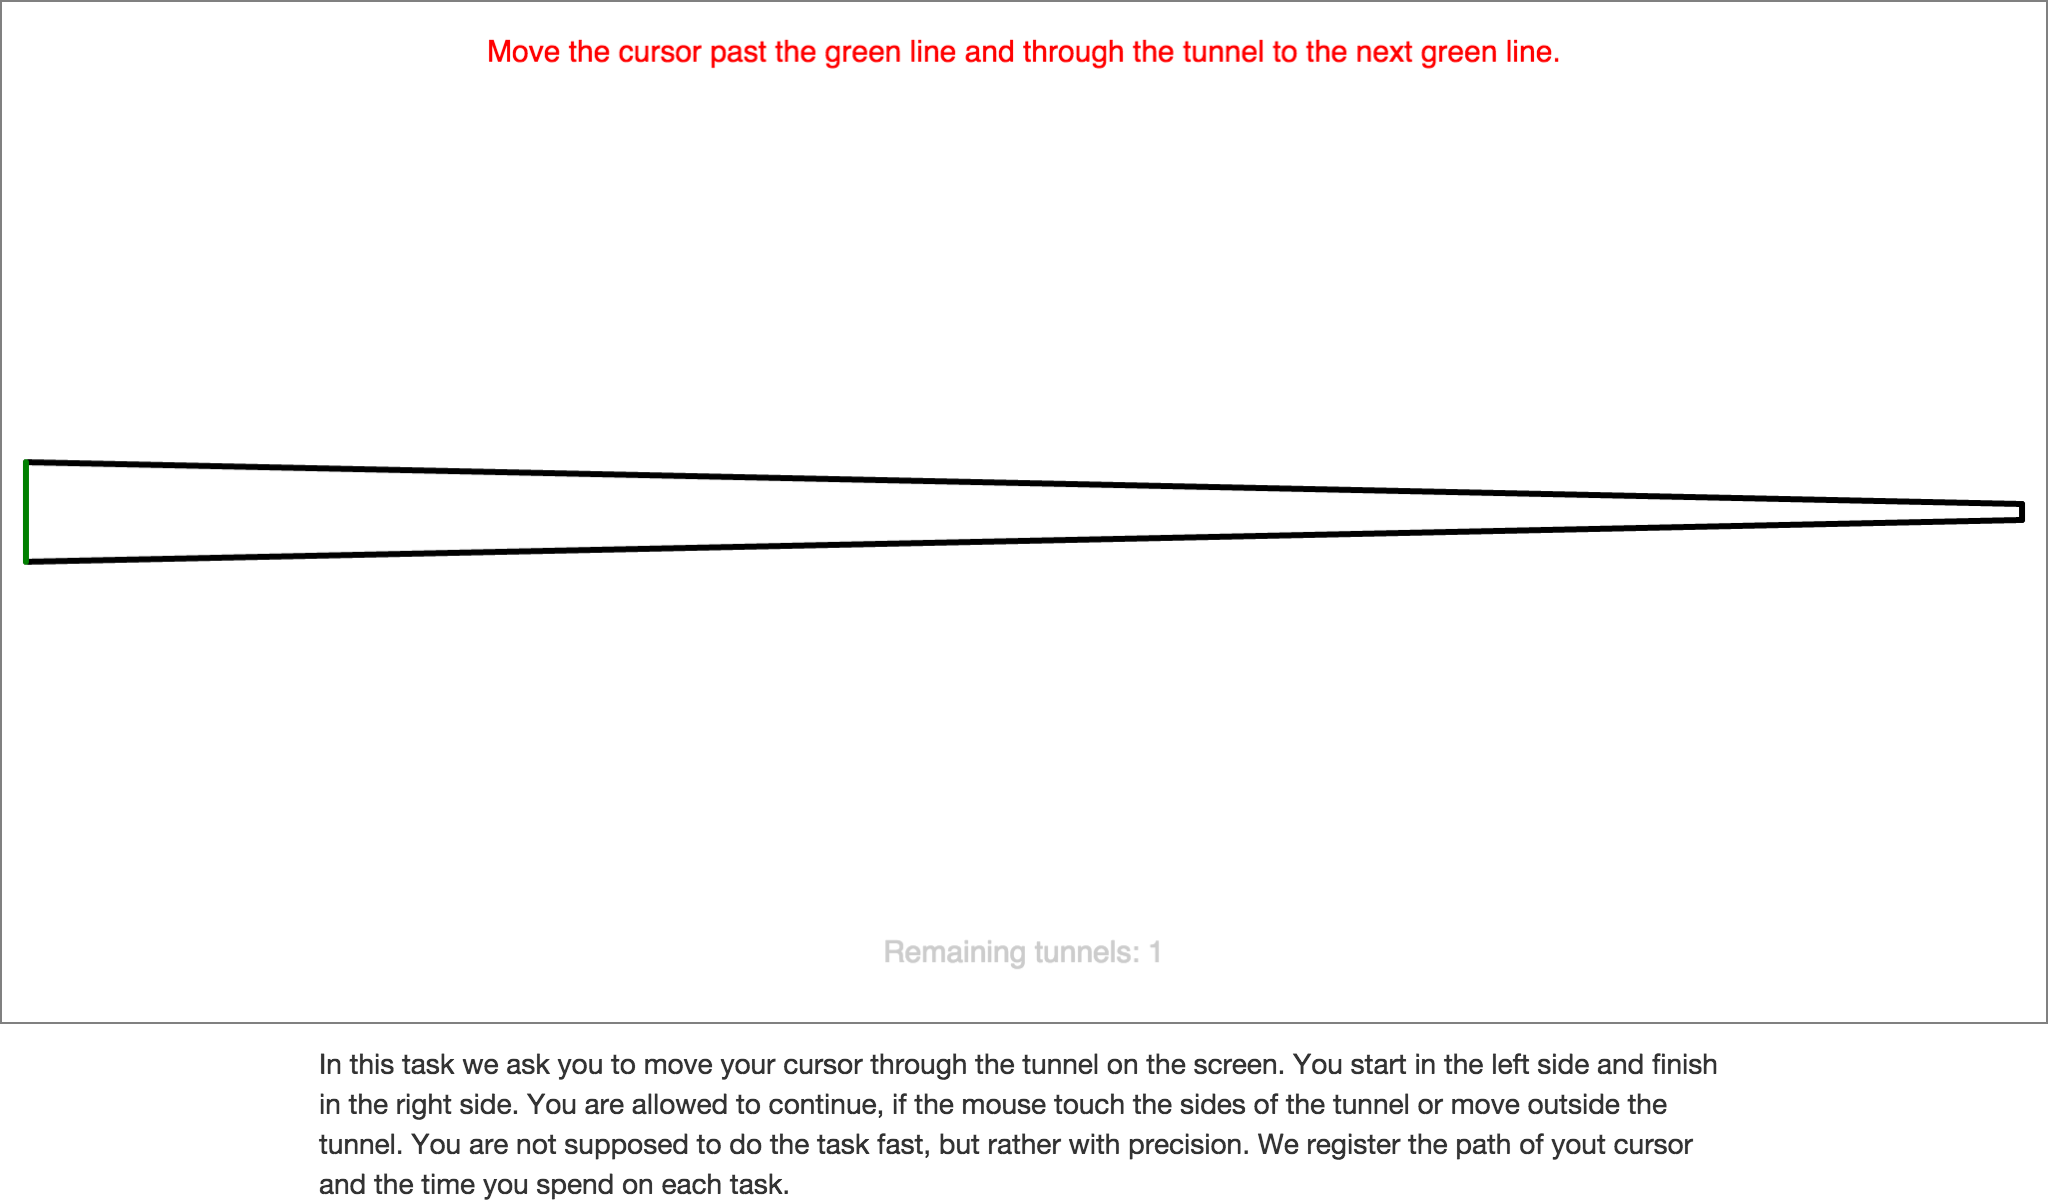
\includegraphics[width=\textwidth, trim = .5cm 20cm .5cm 15cm, clip]{images/screenshots/ex_step_4_tunnel_4}
		\captionof{figure}{Skærmbillede af den fjerde tunnelopgave.}
		\label{fig:ex_tunnel_4}
	\end{minipage}
\end{minipage}\\\\
I denne opgave skal testdeltageren føre deres markør igennem fire tunneller af varierende længe, og varierende indmundingsbredde. Alle tunnellerne er skaleret ned til 50\% af deres oprindelige størrelse, så deres indbyrdes relative størrelse er beholdt. De fire tunneller kan ses på Figur \ref{fig:ex_tunnel_1}, \ref{fig:ex_tunnel_2}, \ref{fig:ex_tunnel_3} og \ref{fig:ex_tunnel_4}.  Størrelserne målt i pixels for tunnellængde ($A$) og den venstre lodrette linje ($W$) er vist i tabel \ref{tab:tunnelopgave}. Den højre lodrette linje er fastsat til 8 pixels bredde, hvilket stemmer overens med forsøget lavet i \cite{accot1997}
\begin{center}
	\begin{tabular}{c c c}
		Tunnel & A & W \\
		\hline
		1 & 100 & 20 \\
		2 & 250 & 30 \\
		3 & 300 & 40 \\
		4 & 400 & 50 \\
	\end{tabular}
	\captionof{table}{Værdier af $A$ (længde) og $W$ (indmundingsbredde) af tunneller brugt i tunnelopgaverne}
	\label{tab:tunnelopgave}
\end{center}
Ved begyndelsen af en tunnelopgave vil den venstre side af tunnellen være markeret med grøn for at tydeliggøre hvor opgaven starter. Når testdeltagerens markør passerer venstre side af tunnellen vil opgaven starte, og det vil nu være den højre side af tunnellen der er grøn, for at signalere hvor markøren nu skal flyttes hen. Når opgaven er i gang, vil der som på figur \ref{fig:ex_tunnel_1} blive vist en grøn linje der hvor markøren flyttes fra, i tilfælde af at testdeltageren rammer eller ryger uden for kanterne, vil de kunne fortsætte ubemærket.\\
Når testpersonen passerer den højre side af tunnellen vil opgaven stoppe, og der vil blive vist en knap hvor testpersonen kan fortsætte til næste opgave, eller afslutte denne test hvis sidste opgave er gennemført. Ved afslutningen af de fire tunnelopgaver vil tunnellernes længde og bredde, og markørens bane, blive gemt - og til sidst sendt til vores database.

\addcontentsline{toc}{subsection}{Spiralopgave}
\subsection*{Spiralopgave}
\begin{minipage}{\linewidth}
	\centering
	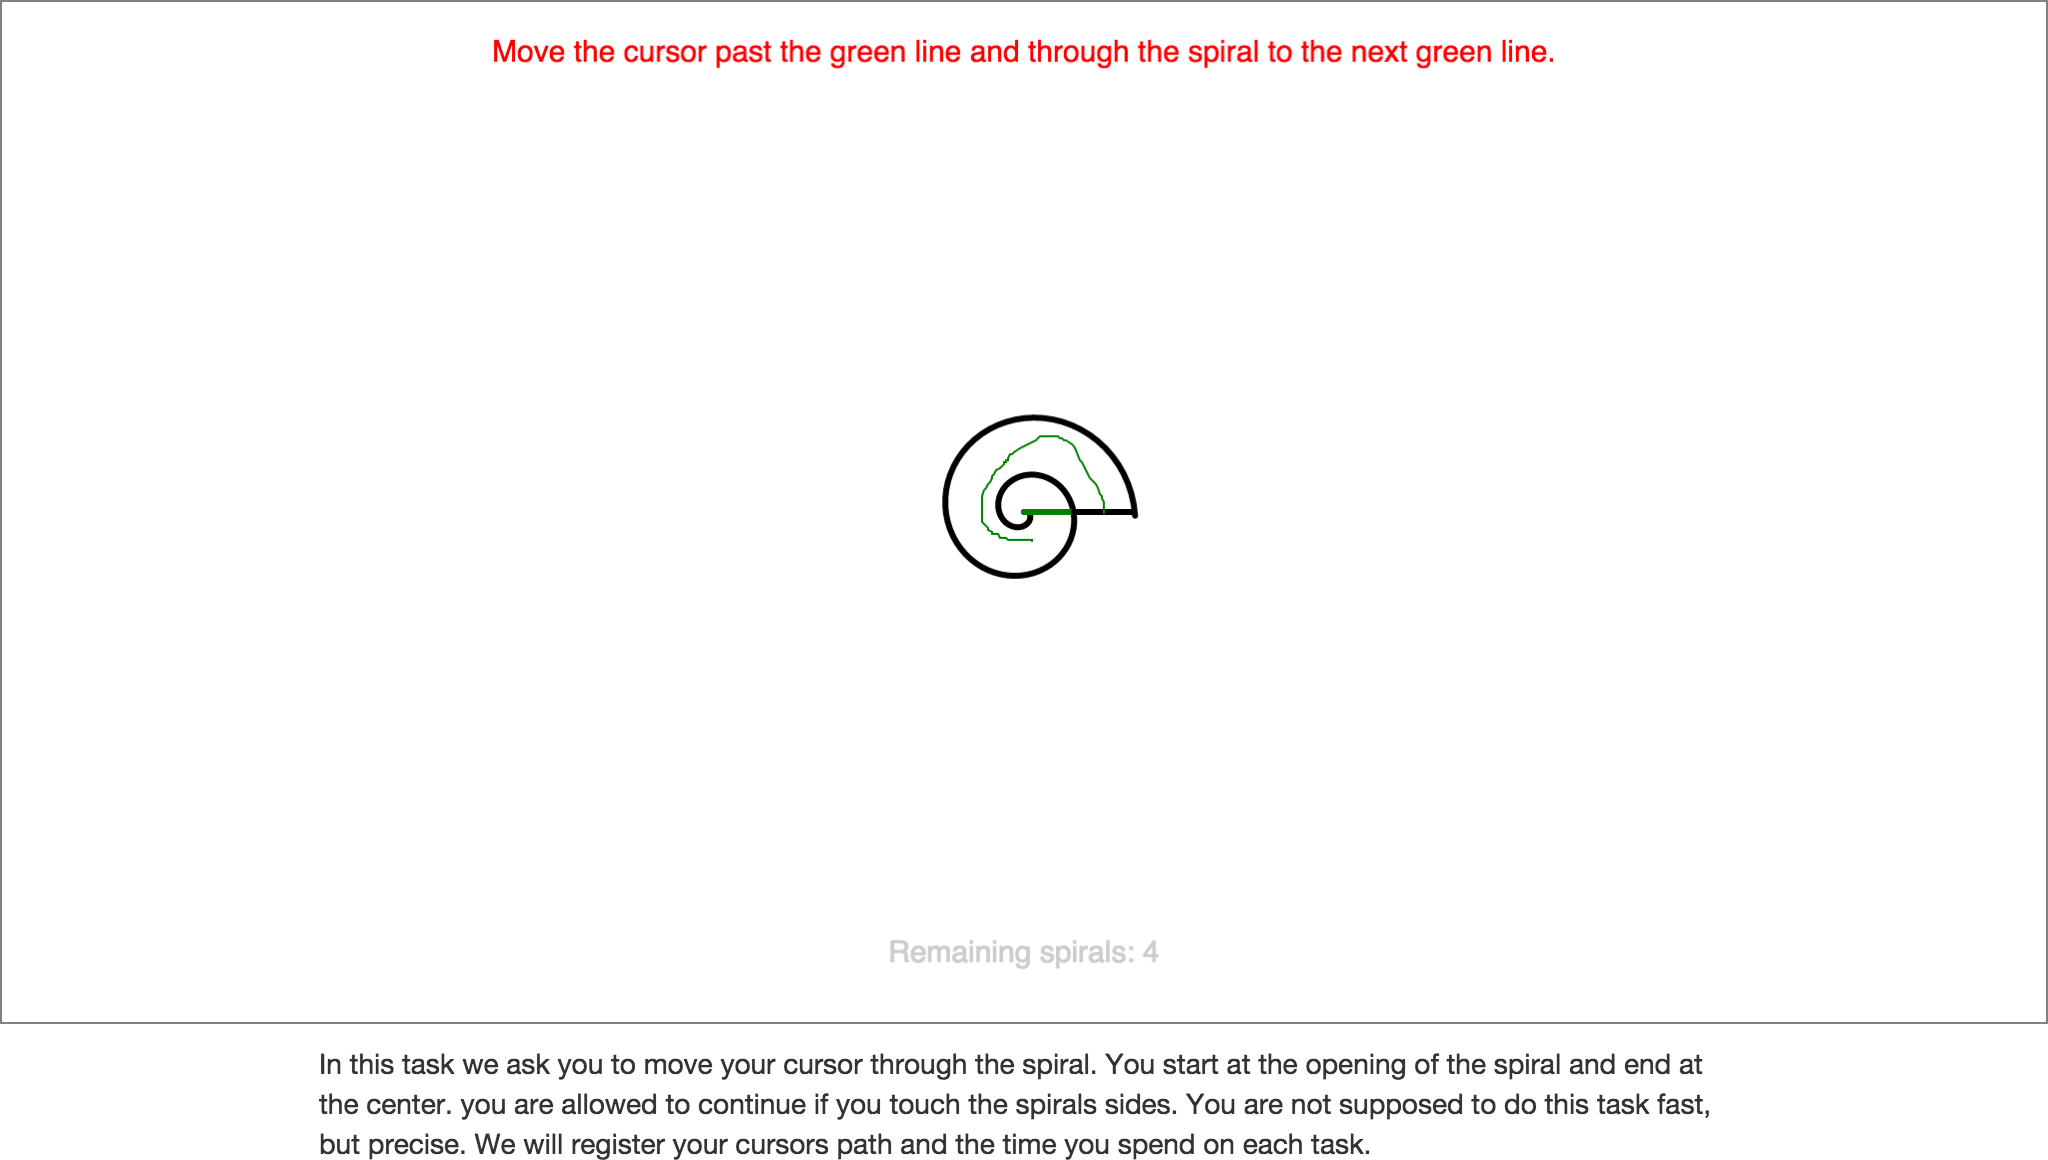
\includegraphics[width=.4\linewidth, trim = 5cm 14cm 5cm 8cm, clip]{images/screenshots/ex_step_5_spiral_path}
	\captionof{figure}{Skærmbillede af den første spiralopgave, med starten af en testpersons sti.}
	\label{fig:ex_spiral_1}
	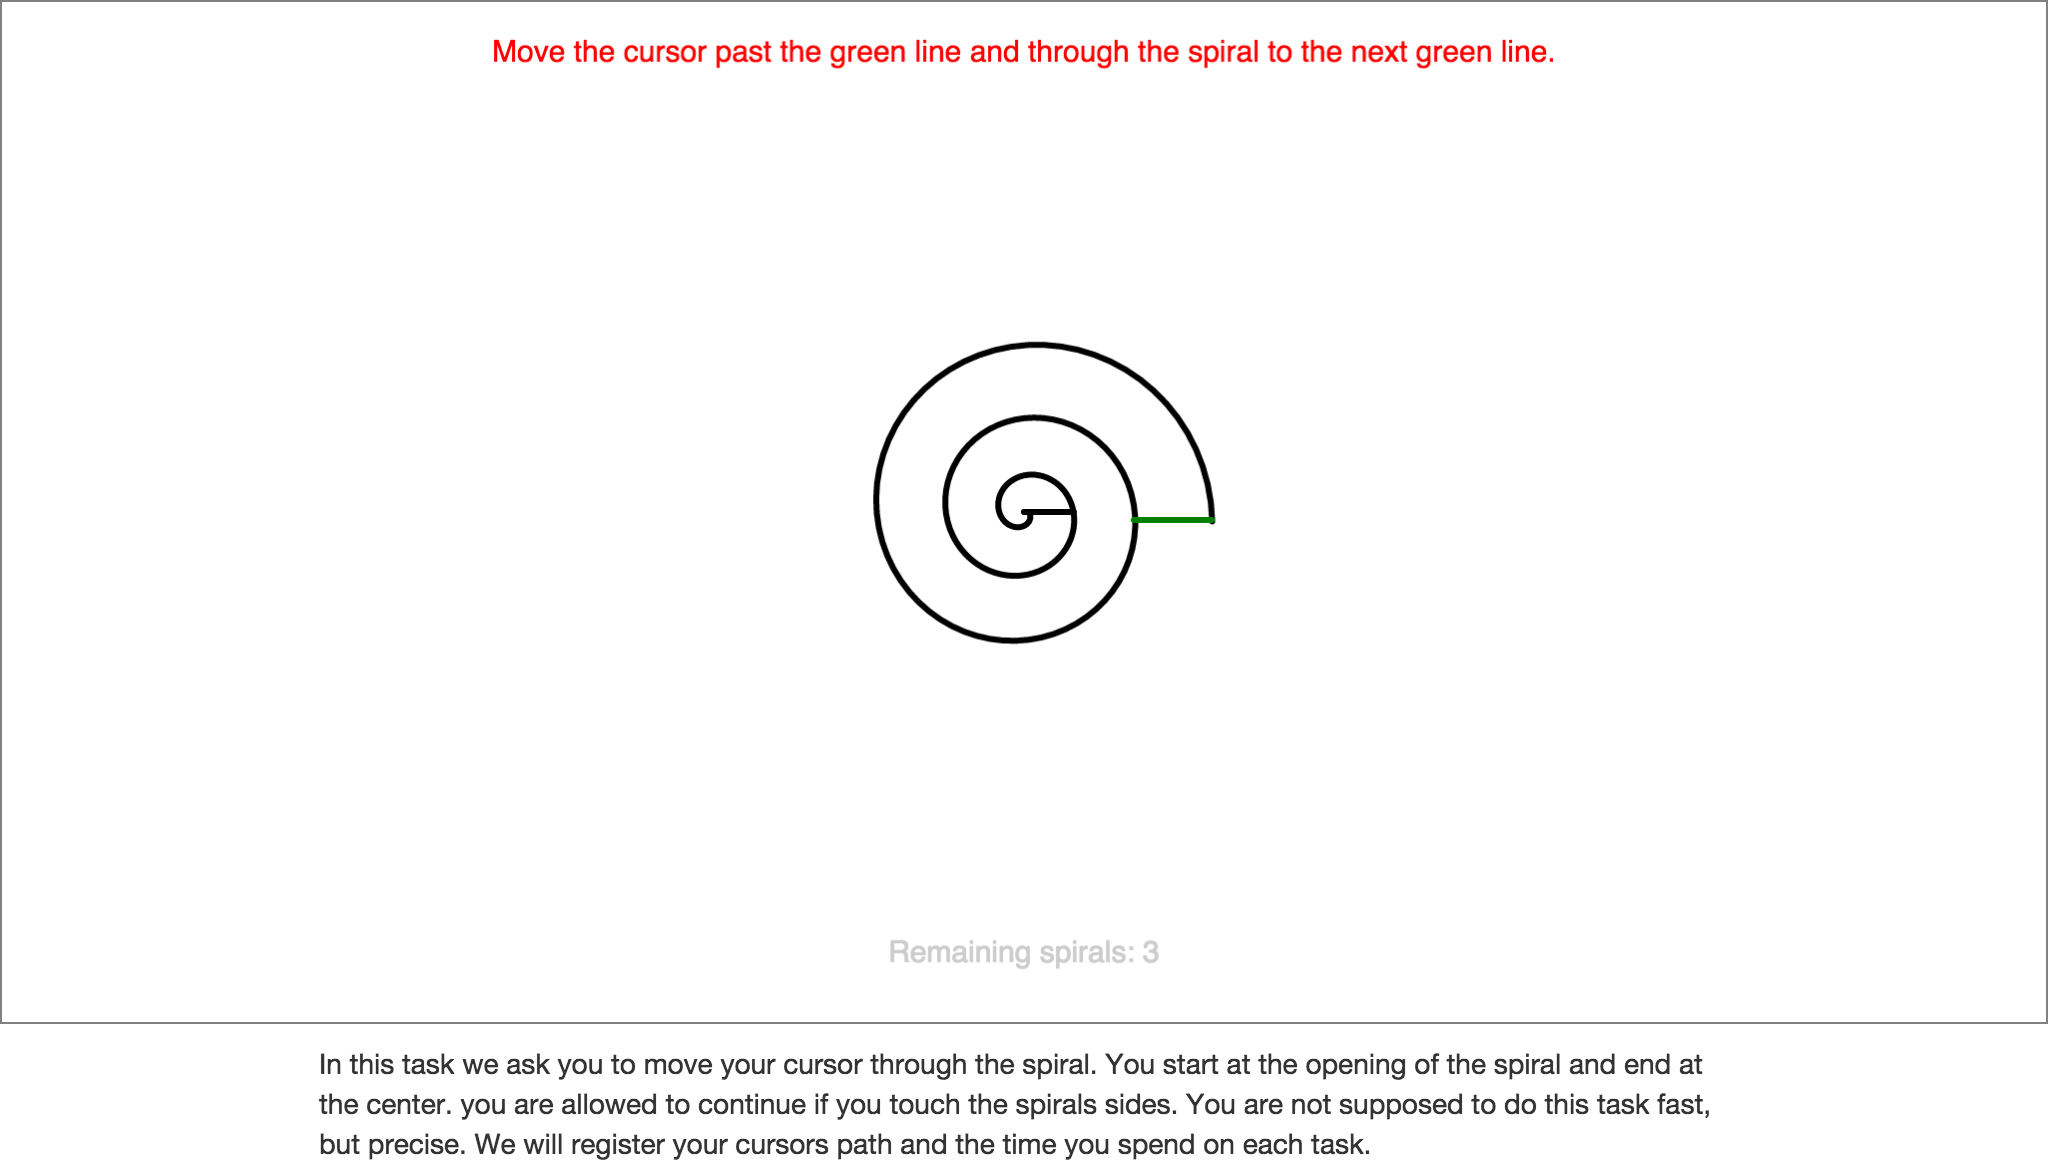
\includegraphics[width=.4\linewidth, trim = 5cm 14cm 5cm 8cm, clip]{images/screenshots/ex_step_5_spiral_2}
	\captionof{figure}{Skærmbillede af den anden spiralopgave.}
	\label{fig:ex_spiral_2}
	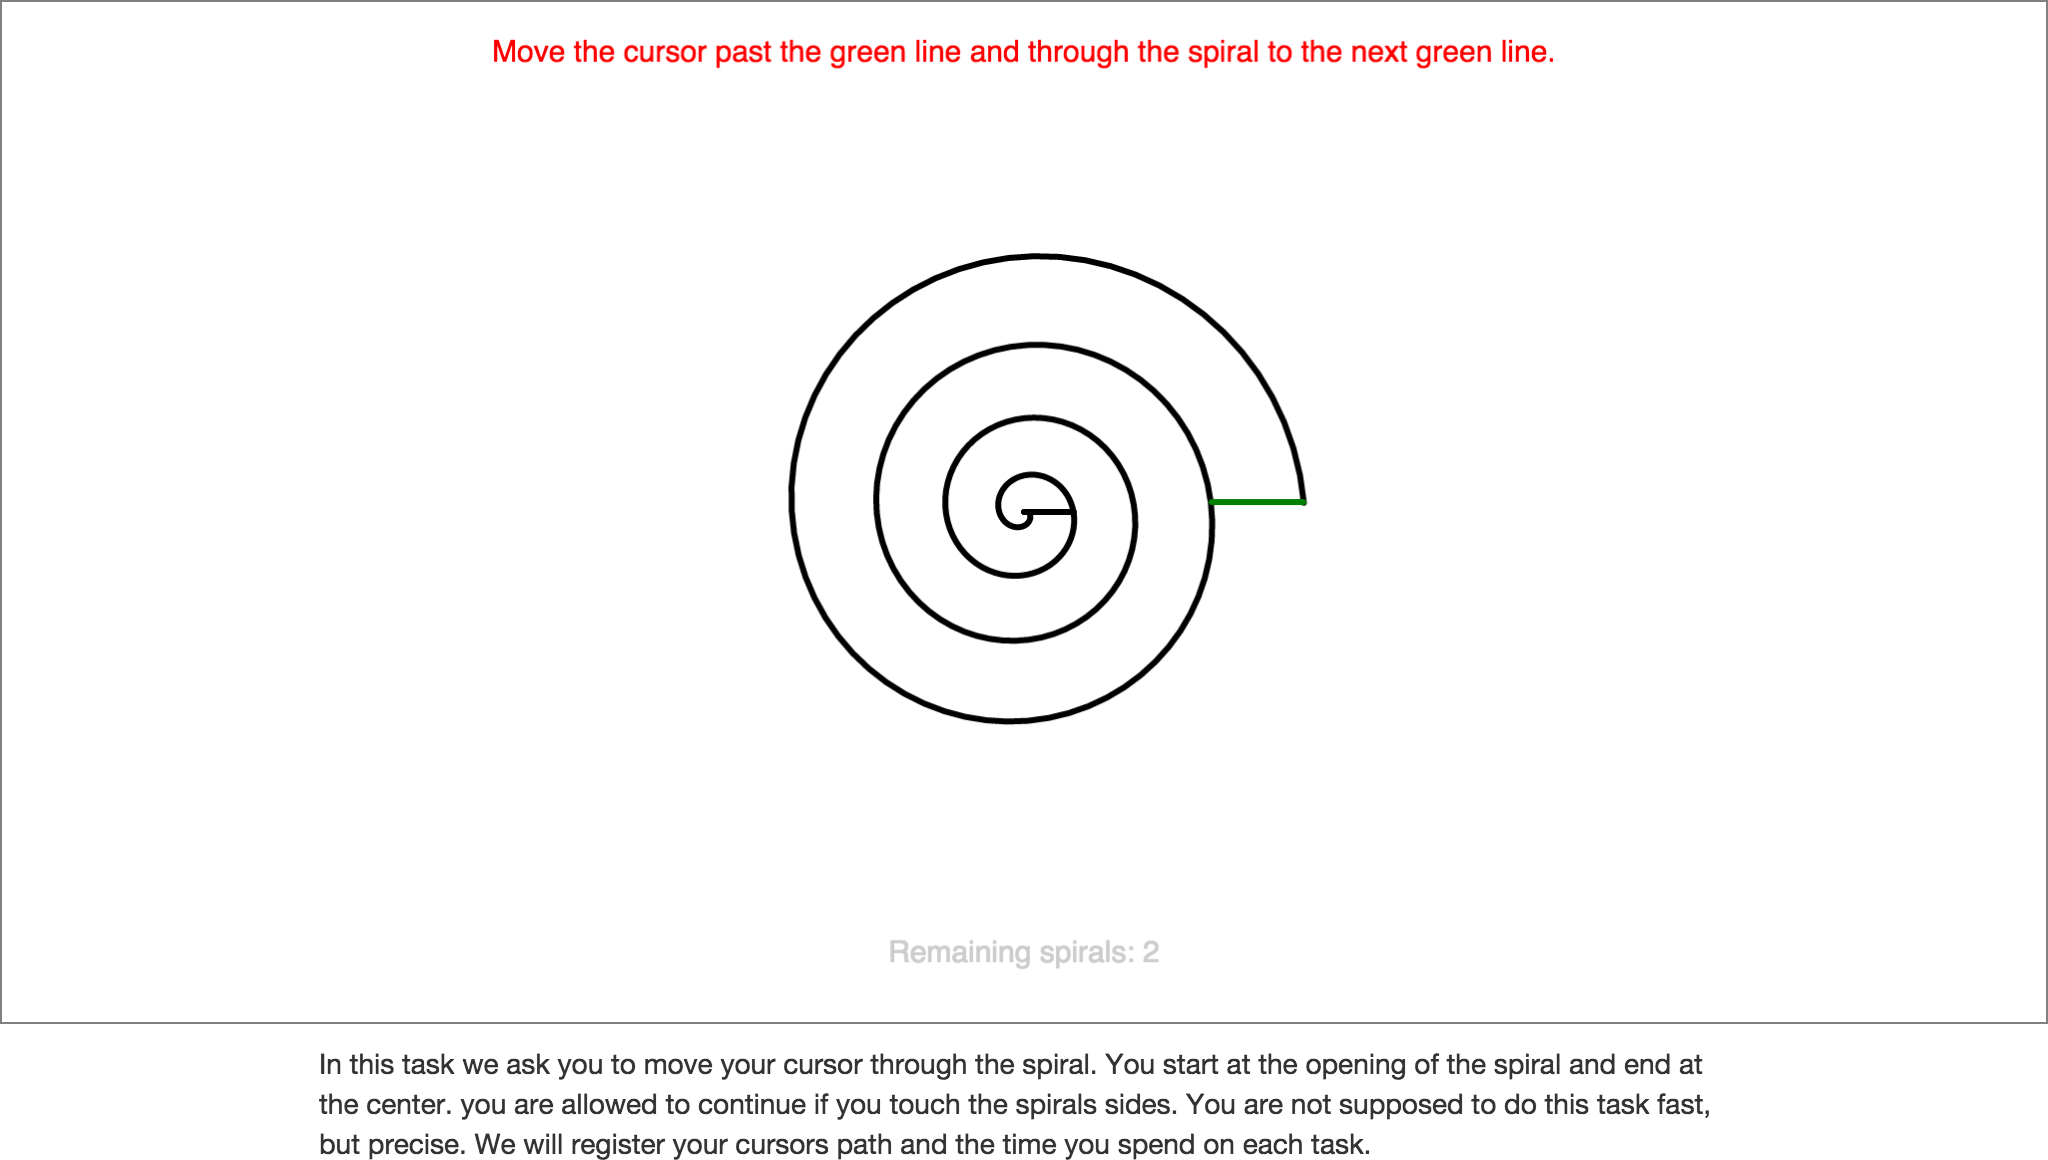
\includegraphics[width=.5\linewidth, trim = 5cm 14cm 5cm 8cm, clip]{images/screenshots/ex_step_5_spiral_3}
	\captionof{figure}{Skærmbillede af den tredje spiralopgave.}
	\label{fig:ex_spiral_3}
	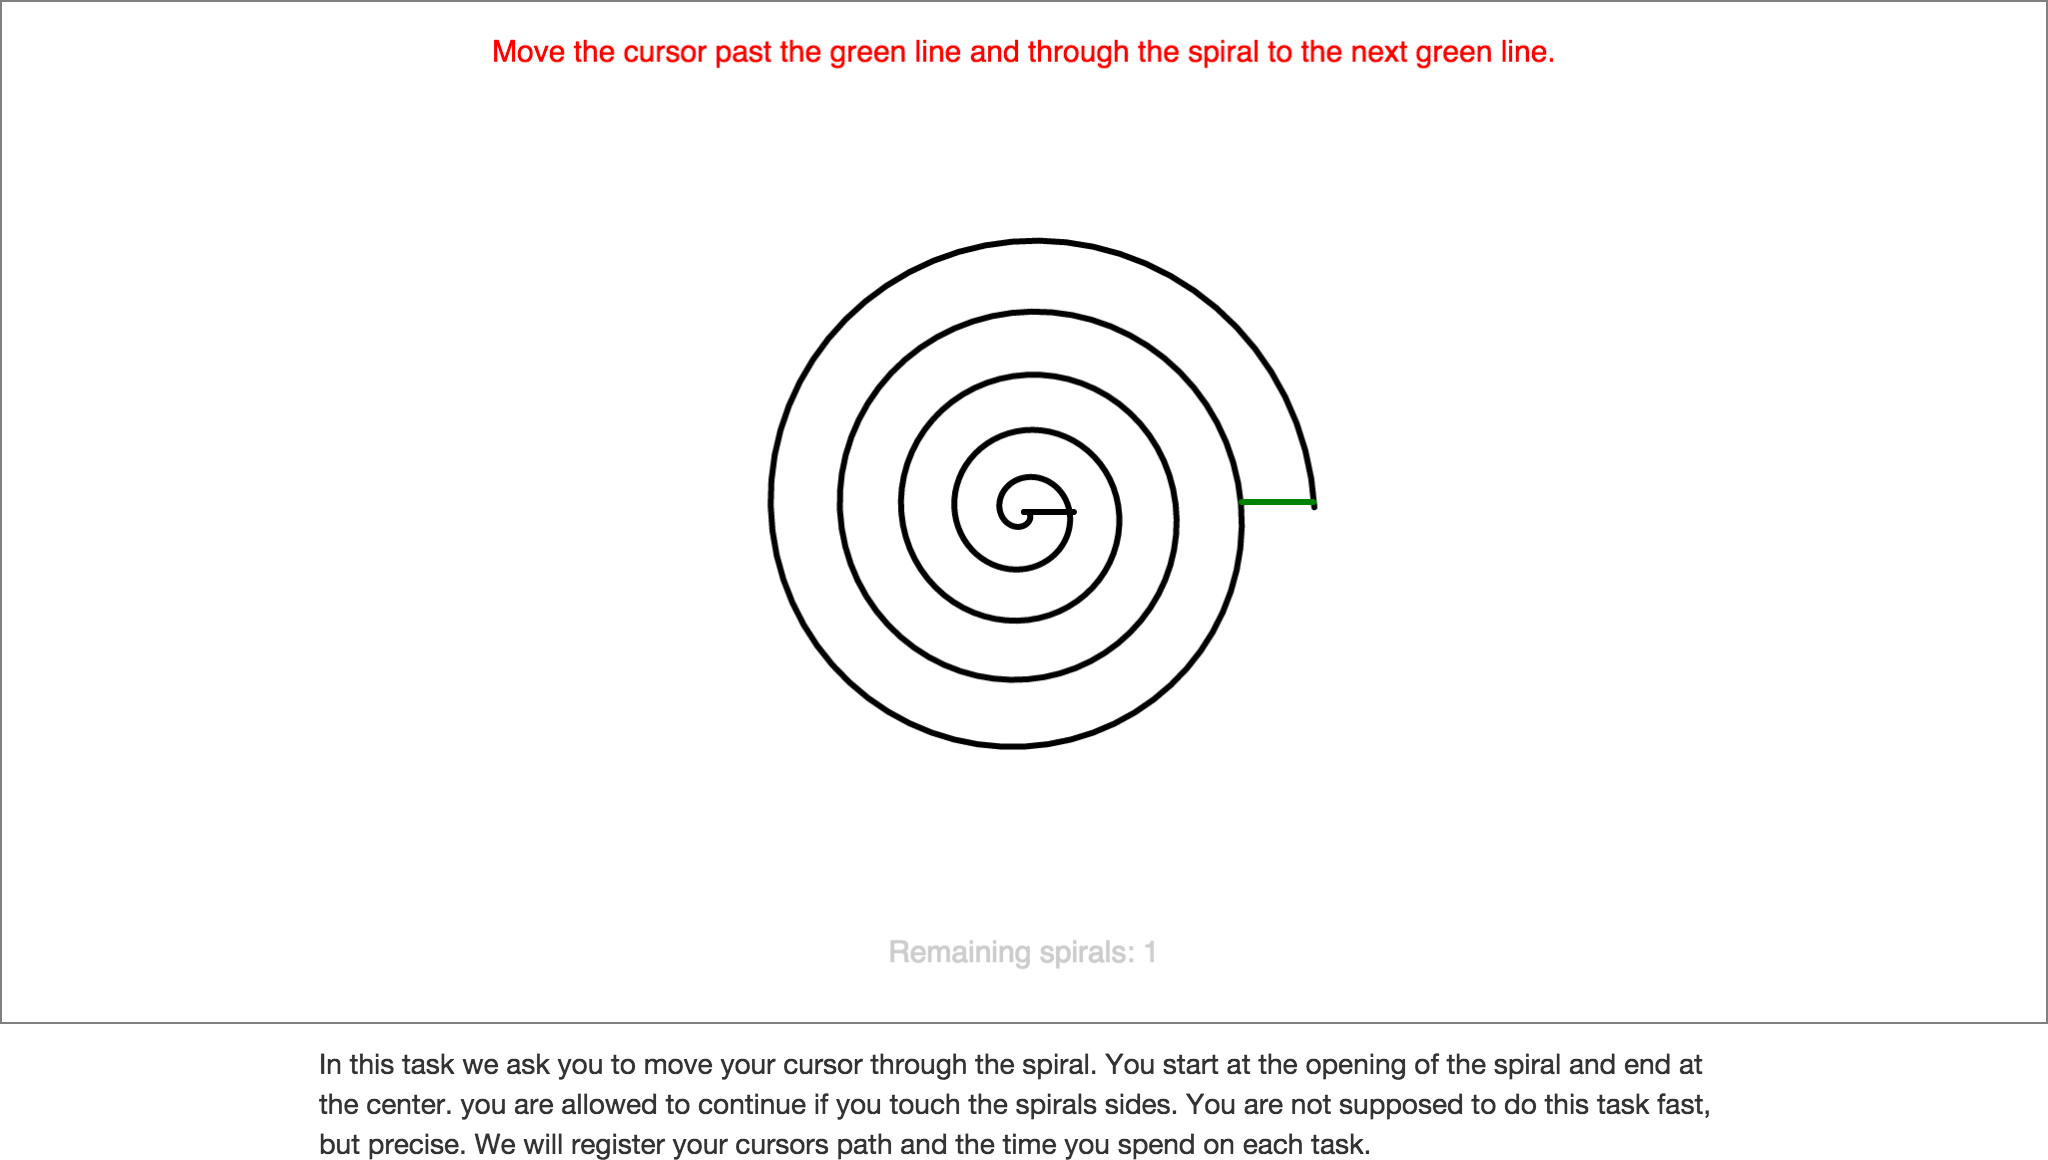
\includegraphics[width=.5\linewidth, trim = 5cm 14cm 5cm 8cm, clip]{images/screenshots/ex_step_5_spiral_4}
	\captionof{figure}{Skærmbillede af den fjerde spiralopgave.}
	\label{fig:ex_spiral_4}
\end{minipage}\\\\
I denne opgave skal testdeltageren føre deres markør igennem fire spiraler af varierende størrelse, og med varierende antal vindinger. De fire spiraler kan ses på figur \ref{fig:ex_spiral_1}, \ref{fig:ex_spiral_2}, \ref{fig:ex_spiral_3} og \ref{fig:ex_spiral_4}. De er skaleret cirka 80\% ned, men deres indbyrdes relative størrelser er beholdt. Antallet af vindinger i spiralerne er vist i figur \ref{tab:spiralopgave}. Antallet af vindingerne på spiralerne er taget fra \cite{accot1997}.
\begin{center}
	\begin{tabular}{c c}
		Spiral & A \\
		\hline
		1 & 1 \\
		2 & 2 \\
		3 & 3 \\
		4 & 4 \\
	\end{tabular}
	\captionof{table}{Værdier af $A$ (antal vindinger) af spiraler brug i spiralopgaverne}
	\label{tab:spiralopgave}
\end{center}
Ved begyndelsen af en spiralopgave vil spiralens udmunding være grøn for at tydeliggøre over for testpersonen hvor opgaven starter. Når testdeltagerens markør passerer den yderste vertikale linje vil opgaven starte, der vil blive vist en grøn streg der, hvor markøren flyttes fra, og den inderste vertikale linje vil derefter skifte til grøn for at signalere hvor testpersonen skal flytte sin markør hen. I tilfælde af at testdeltageren rammer kanten både ind- og udvendigt i spiralen, vil de kunne fortsætte ubemærket.\\
Når testpersonen passerer den inderste vertikale linje i spiralen, vil opgaven stoppe. Der vil efterfølgende blive vist en knap hvor der kan fortsættes til næste spiral, eller afslutte og fortsætte til næste opgave. Ved afslutning af opgaven vil vi, som med tunnelopgaven, gemme tiden det har taget og banen brugt igennem spiralen, og sende denne til vores database.

\addcontentsline{toc}{subsection}{Pegeopgave}
\subsection*{Pegeopgave}
I denne opgave vil testdeltageren blive præsenteret for en sekvens af 25 cirkulære mål af skiftende størrelse og position. Målene præsenteres i rækkefølgen som ses i Tabel \ref{tab:pegeopgave}. Hver test i sættet starter, når testdeltageren klikker inden for en fastplaceret cirkel i vinduets center og slutter når testdeltageren klikker indenfor målet. Hvert cirkulært mål varierer i distance fra center-cirklen og varierer i diameter, hvilket giver ændringer i A/W-sværhedsgrad som ses i tabel \ref{tab:pegeopgave}. Center-cirklen vil blive præsenteret i en grøn farve, se figur \ref{fig:pegeopgave_start}, og vil ved klik skifte til blå - alle mål-cirklerne er vist i grøn farve. Figur \ref{fig:pegeopgave_target} illustrerer, hvordan center- og mål-cirklerne er farvet. 

Testdeltagerens bane til mål-cirklen er illustreret ved en grøn linje, der følger musen, et eksempel herpå ses i figur \ref{fig:pegeopgave_path}. Vi vil i løbet af opgaven registrere tiden det tager fra at testpersonen trykker på center-cirklen, til de trykker på målet. Dertil vil banen som testdeltageren bruger også blive registreret. De tre illustrationer af pegeopgaven er skaleret forskelligt for bedre at tydeliggøre, essensen i opgaven.

\begin{minipage}[t]{.5\linewidth}
\centering
\vspace{0pt}
\captionof{figure}{Illustration af cirklen I midten af skærmen ved pegeopgavens start.}
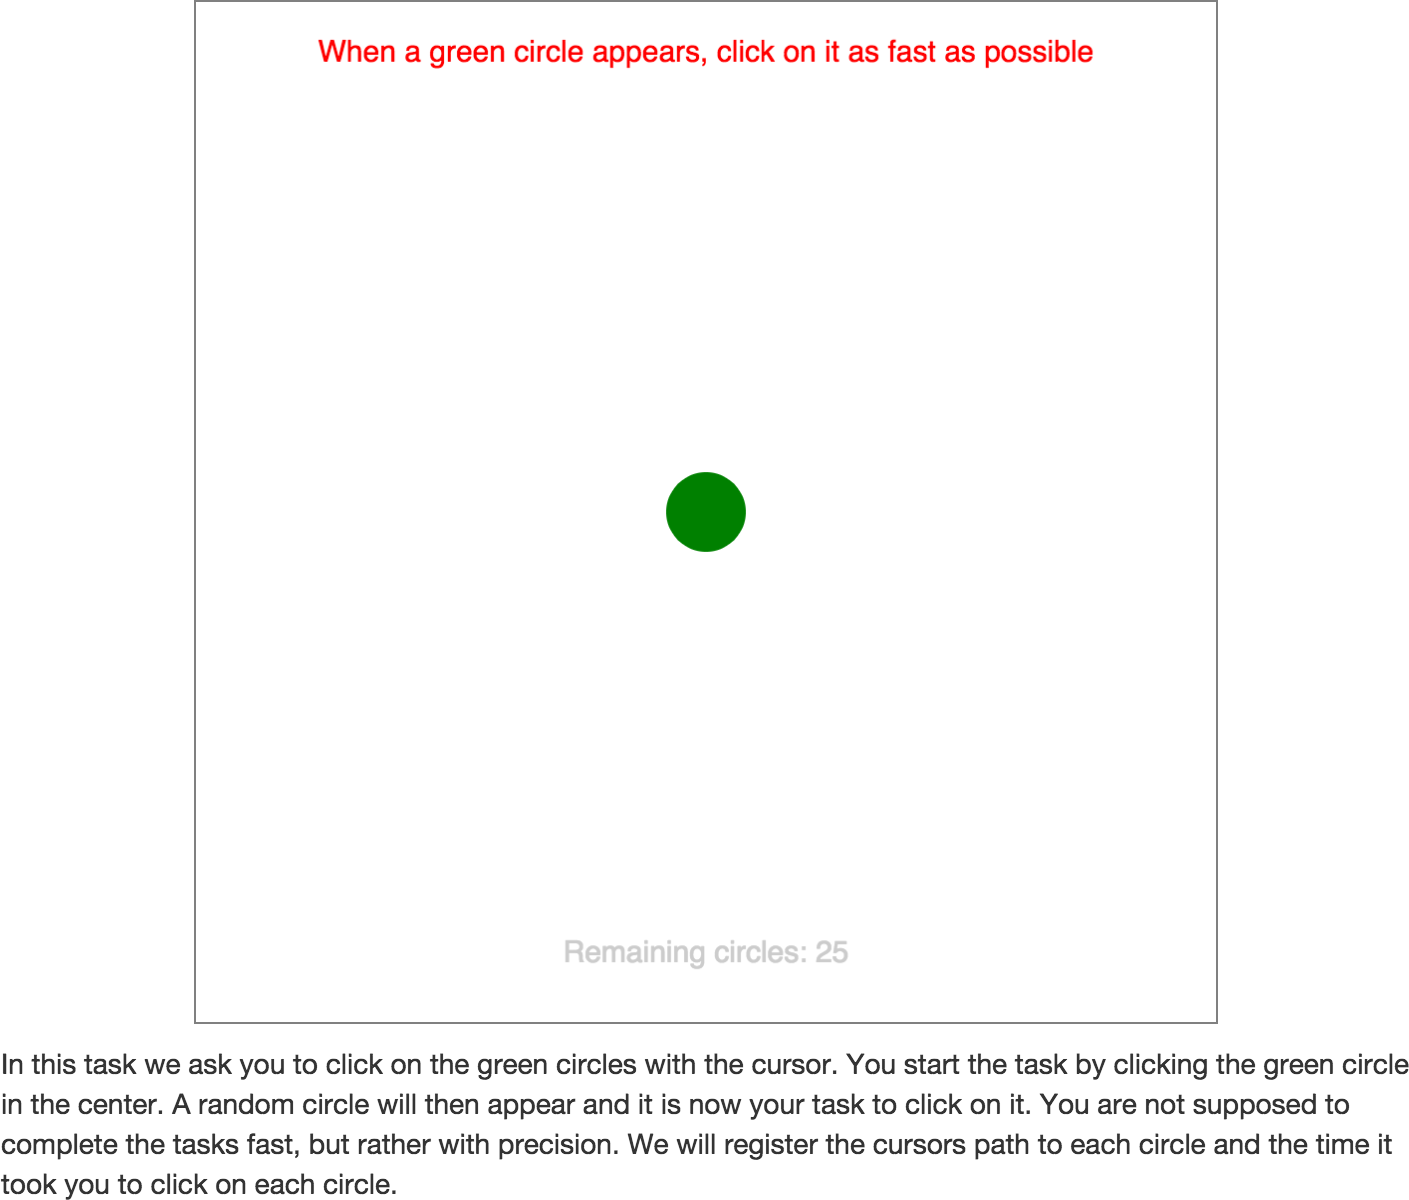
\includegraphics[width=0.8\textwidth, trim = 8cm 20cm 8cm 15cm, clip]{images/screenshots/ex_step_6_pointing_start}
\label{fig:pegeopgave_start}
\caption{Illustration af cirklen I midten, og målet der skal rammes efter der klikkes på cirklen I midten af skærmen.}
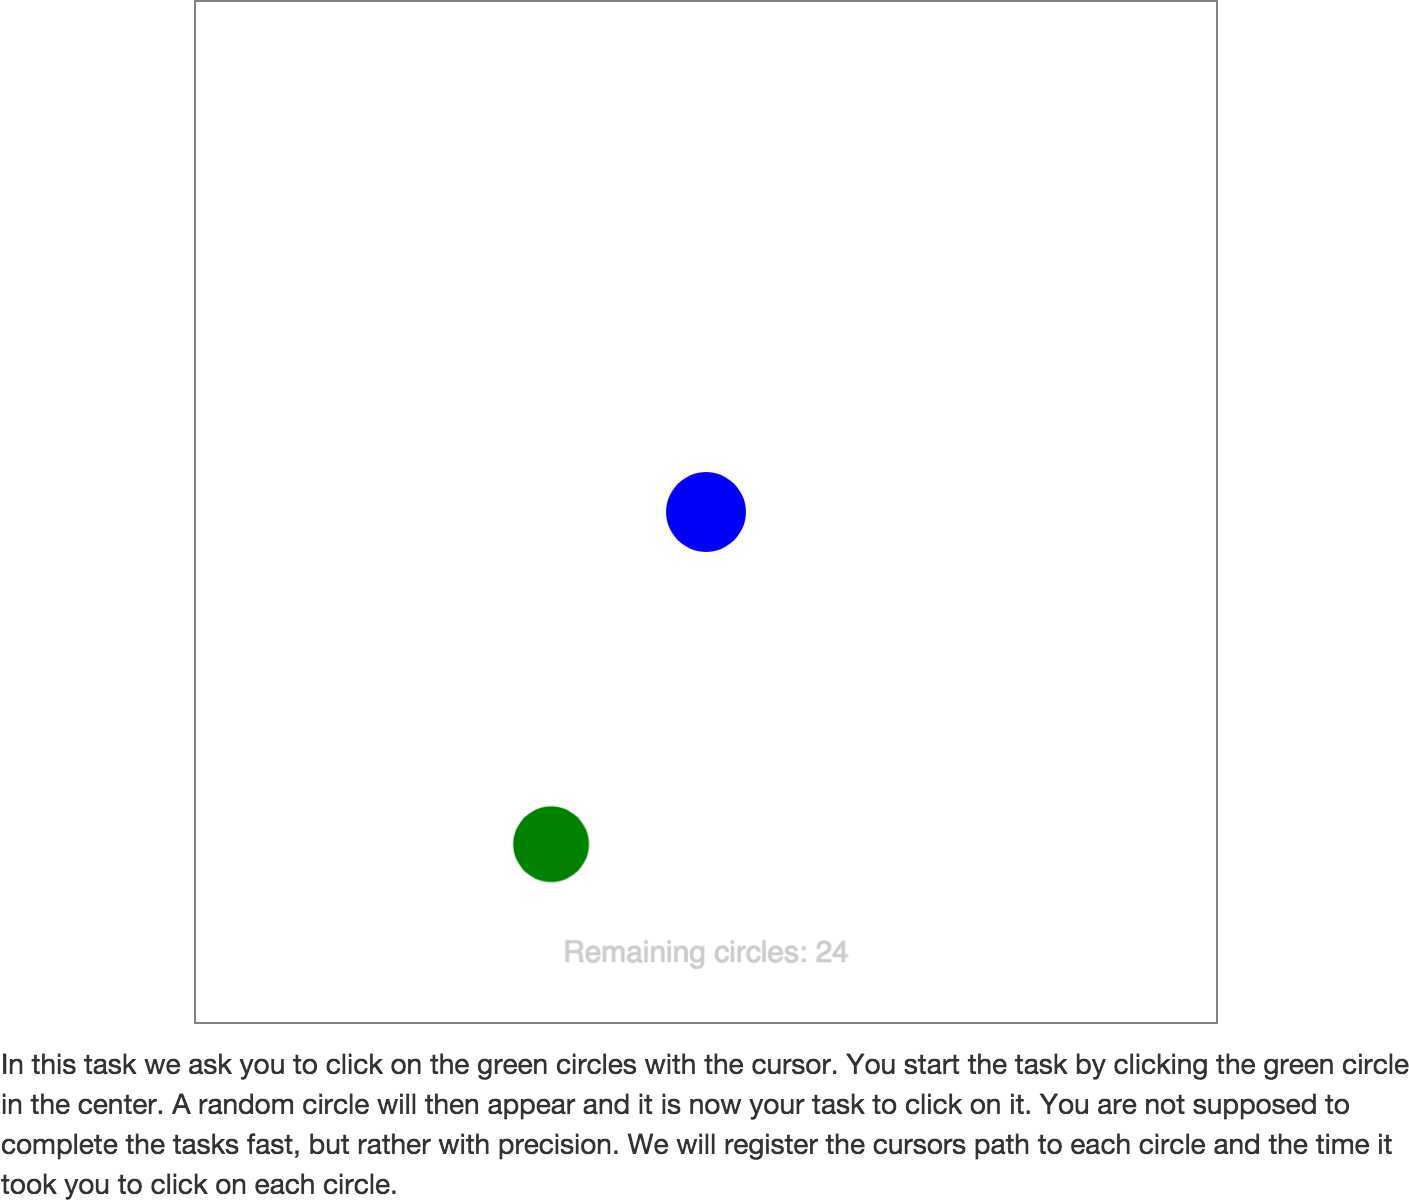
\includegraphics[width=0.8\textwidth, trim = 8cm 8cm 8cm 15cm, clip]{images/screenshots/ex_step_6_pointing_target_1}
\label{fig:pegeopgave_target}
\caption{Illustration af cirklen I midten, målet der skal rammes, og stien som testpersonen har taget for at komme hen til målet}
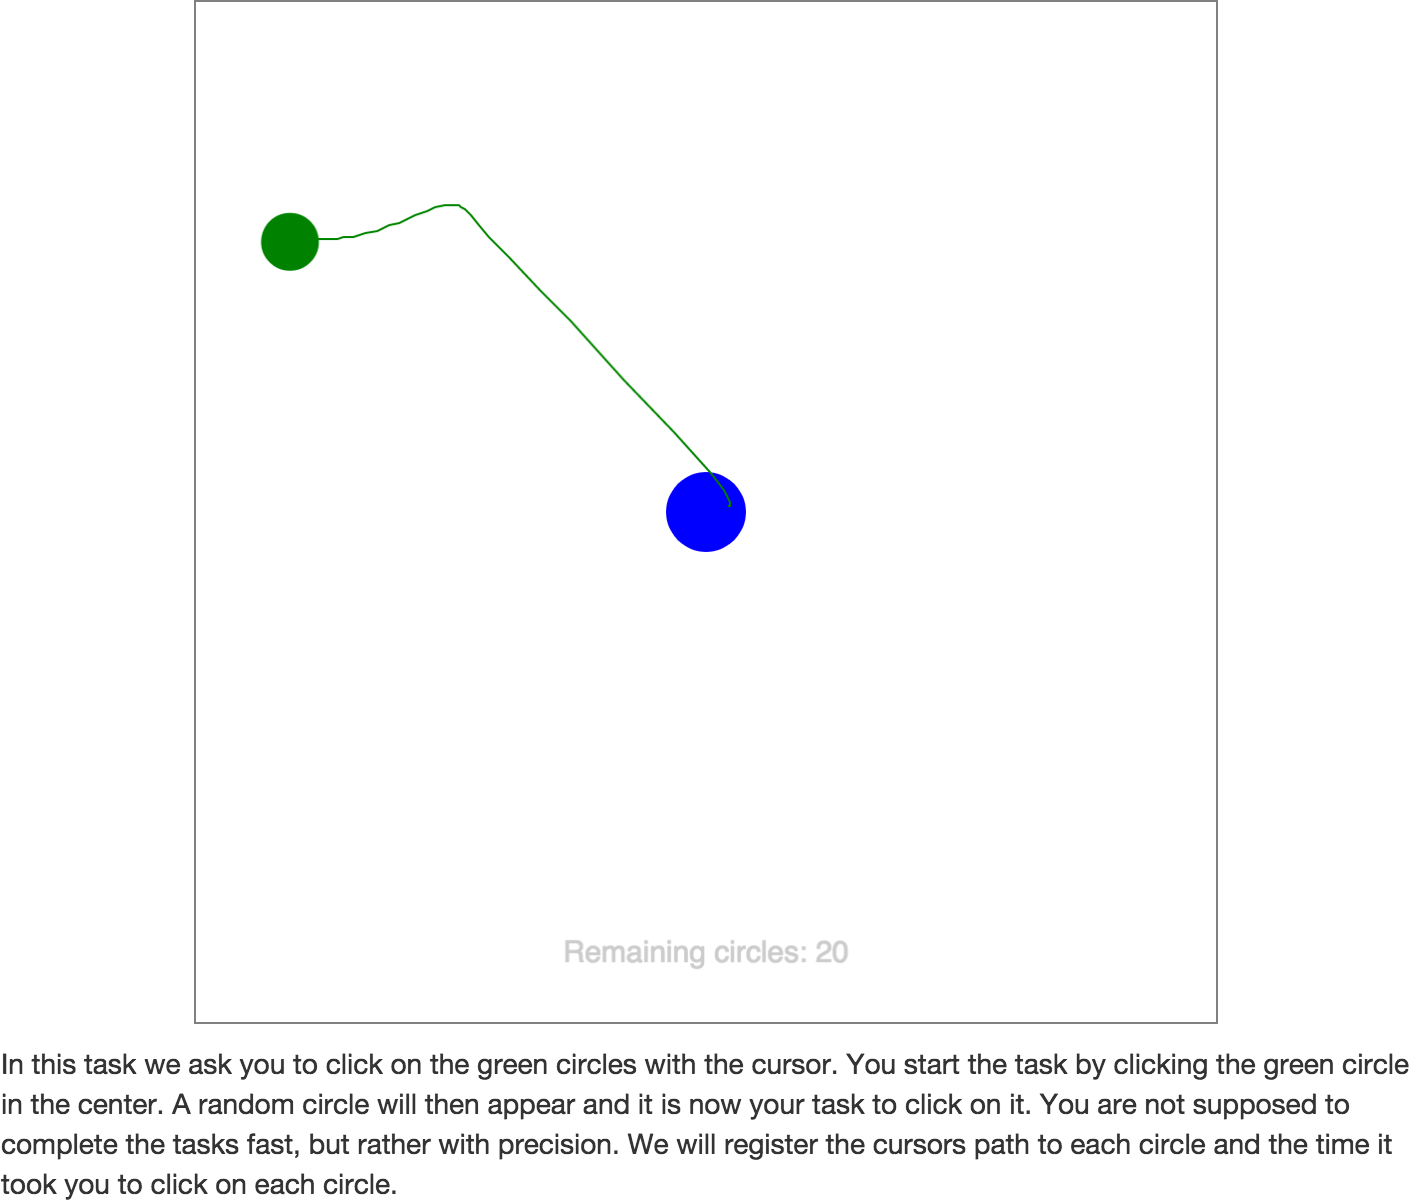
\includegraphics[width=0.8\textwidth, trim = 8cm 22cm 20cm 5cm, clip]{images/screenshots/ex_step_6_pointing_path}
\label{fig:pegeopgave_path}
\end{minipage}
\begin{minipage}[t]{.5\linewidth}
\centering
\vspace{0pt}
    \begin{tabular}{ c c c c }
        Forsøg & $A$ & $W$ & $A/W$ \\\hline
        1  & 67  & 20 & 3.35  \\
        2  & 184 & 38 & 4.84  \\
        3  & 280 & 14 & 20.00 \\
        4  & 230 & 29 & 7.93  \\
        5  & 144 & 55 & 2.62  \\
        6  & 249 & 29 & 8.59  \\
        7  & 255 & 14 & 18.21 \\
        8  & 96  & 50 & 1.92  \\
        9  & 225 & 19 & 11.84 \\
        10 & 263 & 12 & 21.92 \\
        11 & 259 & 25 & 10.36 \\
        12 & 229 & 20 & 11.45 \\
        13 & 215 & 31 & 6.94  \\
        14 & 198 & 83 & 2.39  \\
        15 & 301 & 16 & 18.81 \\
        16 & 194 & 66 & 2.94  \\
        17 & 260 & 12 & 21.67 \\
        18 & 296 & 14 & 21.14 \\
        19 & 180 & 44 & 4.09  \\
        20 & 278 & 11 & 25.27 \\
        21 & 283 & 37 & 7.65  \\
        22 & 40  & 32 & 1.25  \\
        23 & 233 & 10 & 23.30 \\
        24 & 191 & 50 & 3.82  \\
        25 & 179 & 18 & 9.94  \\\hline
    \end{tabular}
   \captionof{table}{Værdier af $A$ (længde til mål), $W$ (bredde af mål) og udregnede $A/W$ for alle pegeopgaver.}
   \label{tab:pegeopgave}
\end{minipage}

\newpage
\addcontentsline{toc}{subsection}{Generelt for de tre opgaver}
\subsection*{Generelt for de tre opgaver}
I alle opgaverne vil deltagerne blive informeret om, hvor mange opgaver de mangler at gennemføre, så de ved hvornår de er færdige, den grå tekst \textit{"Remaining circles"} i figur \ref{fig:pegeopgave_target} er et eksempel på, hvordan denne information så ud undervejs. Vi har medtaget det i håb om, at testdeltagere fra crowdsourcing forsøget ikke vil miste tålmodigheden midt i testen.  

Hvis deltagerne bevæger pegeenheden uden for det canvas som opgaven skal udføres i vil denne del af banen ikke komme med i vores gemte data. For tunnel og spiralopgaverne er størrelsen på det omkring liggende canvas 1024x512 pixels, imens det for pegeopgaven er 512x512 pixels. Disse størrelser er faste uanset størrelsen på testdeltagerens skærm.

\addcontentsline{toc}{chapter}{Eksperimenter}
\chapter*{Eksperimenter}

\addcontentsline{toc}{section}{Udførsel af eksperimenter}
\section*{Udførsel af eksperimenter}

\addcontentsline{toc}{subsection}{Laboratorieeksperiment}
\subsection*{Laboratorieeksperiment}
Laboratorieeksperimentet vil blive udført af 10 tilfældigt udvalgte universitetsstuderende - dog ikke dataloger.
Forsøget foretages fra kl 9-13 - tidligt på dagen - for at sikre, at folk stadig er friske. Det vil foregå i en 4-personers sofabås på H.C. Ørstedsinstituttet, hvor der er privat og uden forstyrrelser.
Tidsmæssigt vil der være afsat 20 minutter til hver deltager, dog med plads til ekstra tid hvis nødvendigt.
Hver deltager bliver først introduceret til vores projekt og derefter introduceret til hhv. tunnel-, spiral- og pegeopgaven.
Herefter bliver testdeltageren bedt om at udføre tunnelopgaven - efterfulgt af spiral- og pegeopgaven - hvor der vil være et antal opgaver som skal udføres, hhv. 4 for tunnelopgaven, 4 for spiralopgaven og 25 for pegeopgaven.

\addcontentsline{toc}{subsection}{Crowdsourcingeksperiment}
\subsection*{Crowdsourcingeksperiment}
Crowdsourcingeksperimentet vil foregå på internettet, og vi har derfor gjort vores program tilgængeligt online. På grund af de faste canvas størrelser vil alle besøg fra smartphones eller tablets blive blokeret, og informeret om, at forsøget kun er tilgængeligt fra en computer. 

Ved crowdsourcingeksperimentets start vil hver deltager udfylde formularen, som ses i Figur \ref{fig:Questions}, før de kan fortsætte. Når formularen er udfyldt forsætter deltageren til opgaverne. Her skal der, ligesom laboratorieeksperimentet, udføres 4 spiralopgaver, efterfulgt af 4 tunnelopgaver og til sidst 25 pegeopgaver. Efter deltageren har udført alle opgaver vil deres data blive sendt til en server, hvorefter deltageren får en informationsmeddelelse.
Vi har valgt at dele vores eksperiment på et antal af reddit-sider, da det er et meget populært internetfora og muliggør, at vi kan nå ud til så mange mennesker som overhovedet muligt.
\begin{itemize}
\item reddit.com/r/denmark\\
Vi valgte $/r/denmark$ fordi det er et aktivt subreddit, som passer til vores forespørgsel, med næsten hundredetusind unikke visninger per måned.
\end{itemize}
For at nå ud til andet end danske brugere har vi valgt også at bruge de to følgende subreddits. De er beregnet til at spørge folk om hjælp, og er de to største med dette formål som vi kunne finde.
\begin{itemize}
\item reddit.com/r/helpme
\item reddit.com/r/care
\end{itemize}

Som det sidste vil vi også dele forsøget på vores egne Facebook-profiler.
\begin{figure}[h]
\centering
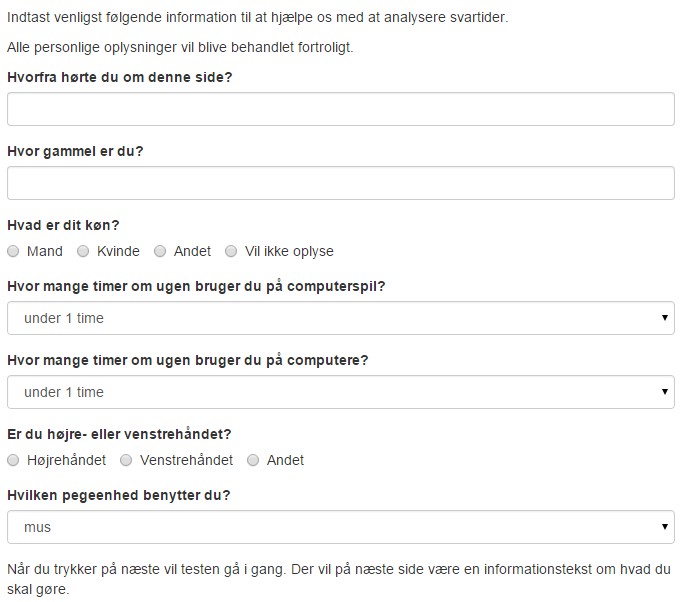
\includegraphics[width=.5\linewidth, trim = 0cm 0cm 7cm 0cm, clip]{images/screenshots/ex_questions}
\caption{Skærmbillede af spørgsmål som blev stillet før crowdsourcing-deltagerne kunne udføre forsøget.}
\label{fig:Questions}
\end{figure}

\addcontentsline{toc}{section}{Resultat af eksperimenter}
\section*{Resultat af eksperimenter}

\addcontentsline{toc}{subsection}{Laboratorieeksperiment}
\subsection*{Laboratorieeksperiment}
Vi, P1, P2 og P3, udførte vores laboratorieeksperiment den 20. april 2015 på H.C. Ørsted instituttet. På trods af, at der på dagen ikke var mange mennesker til stede, så fik vi alligevel 10 personer igennem vores eksperiment i løbet af fire timer. De 10 testdeltagere var af varierende køn og nationalitet. Alle testdeltagere blev hvervet af P1 og blev derefter introduceret til eksperimentet af enten P2 eller P3. Herefter udførte alle testdeltagere forsøget uden behov for yderlig assistance. Testdeltagerne syntes godt om forsøget. Alt i alt forløb vores forsøg som forventet, uden problemer eller forstyrrelser.

\addcontentsline{toc}{subsection}{Crowdsourcingeksperiment}
\subsection*{Crowdsourcingeksperiment}
Forsøget gik godt - 264 personer gennemførte vores forsøg og har suppleret os med vital data. Vi fik delt vores forsøg på størstedelen af de tidligere beskrevne sider, dog med nogle få undtagelser. Generelt set var reddit det mest lukrative sted, hvorfra 140 personer har skrevet siden på som deres reference - hvorimod 74 skrev at de var blevet refereret fra Facebook.\\
Det var ikke muligt at dele vores forsøg på $reddit.com/r/helpme$ og $reddit.com/r/care$, da vi ikke havde nok "karma"-point til at kunne lave et indlæg på disse sites.\\
Efterfølgende har vi lukket for muligheden for at deltage i vores forsøg den 30/04/2015, og skrevet en besked på forsøgssiden hvor vi takker folk for deres deltagelse.

\addcontentsline{toc}{chapter}{Analyse}
\chapter*{Analyse}
I dette afsnit vil vi analysere den indsamlede data ved brug af både kvantitative og kvalitative metoder. Vi vil mere præcist analysere testdeltagernes bevægelsesbaner og hastighedsprofiler. 
\addcontentsline{toc}{section}{Modeludvælgelse}
\section*{Modeludvælgelse}
Som det kan ses af de fire formuleringer for Fitts' lov, så kan de alle sammen opfattes som affine modeller, med tiden $T$ som y-variabel og ID som x-variabel. Bemærk, at Welfords formel har en skæring med y-aksen i 0, dvs. $y=b\cdot x$.

For at kunne finde ud af hvilken af de fire lineære modeller der beskriver vores data bedst, har vi taget udgangspunkt i \cite{wu2011experiments} der refererer til tre modeludvælgelseskriterier som værende almindeligt anvendte.

I \cite{wu2011experiments} afsnit 1.7 bliver $C_p$, $AIC$ og $BIC$ beskrevet som almindeligt anvendte, og der bliver refereret til Ockhams ragekniv som værende et godt udgangspunkt ved modeludvælgelse, da det oftest er den simpleste model der passer bedst. Dette har vi brugt til selv at vælge $LSE$, da denne er simpel, og derfor er understøttet som metode, af Ockhams ragekniv.
\begin{itemize}
\item{Least Squared Errors (LSE) \cite{legendre1805}.}
\item{Mallow's $C_p$ \cite{mallow1973}.}
\item{Akaike Information Criterion (AIC) \cite{akaike1973}.}
\item{Bayesian Information Criterion (BIC) \cite{schwarz1978}.}
\end{itemize}
LSE er bestemt ved at finde gennemsnittet af kvadratet på afstandene fra punkterne til modellen, den model som har det laveste gennemsnit bliver vurderet som bedst. Et problem ved udelukkende at benytte dette kriterium er, at en model altid kan beskrive alle datapunkter perfekt ved blot at inkludere flere parametre. Således, at modellen bliver et polynomium af højere grad end det originale, dette kaldes overfitting.

Mallow's $C_p$ kriteriet bliver beregnet ud fra LSE men inddrager også antallet af parametre i beregningen for netop at undgå overfitting. Tilsvarende gør sig gældende for AIC og BIC, de beregnes dog ved hjælp af maximum likelihood i stedet for LSE.

For et givent datasæt $x$ og en tilhørende statistisk model vil likelihoodfunktionen beregne sandsynligheden for at modellens parametre $p$ vil resultere i $x$. Ved maximum likelihood findes de værdier for parametrene $p$, som maksimere likelihood funktionen. Det vil sige de værdier for parametrene $p$, som gør det observerede datasæt $x$ mest sandsynligt. Forskellen på AIC og BIC er, at BIC vægter antallet af parametre mere negativt end AIC.

Af de fire beskrevne modeller har vi valgt at bruge AIC, da det er den mest udbredte at basere sin modeludvælgelse på. Hvis vi lader $L$ være maximum likelihood-værdierne for modellens parametre og $k$ antallet af parametre, så er AIC givet ved
\begin{align}
AIC = 2k - 2\ln(L) \label{eq:aic}
\end{align}
Vi har til vores analyse brugt programmeringssproget R, som både har lineær regression og AIC-funktionalitet indbygget. $lm()$\footnote{R dokumentation om $lm()$: \url{https://stat.ethz.ch/R-manual/R-patched/library/stats/html/lm.html}} fitter en lineær model ud fra de (x,y) datasæt der gives som input. Modellen bliver baseret på least squares, og kan også tvinges til at gå igennem origo (for Welford).

$AIC()$\footnote{R dokumentation om $AIC()$: \url{https://stat.ethz.ch/R-manual/R-patched/library/stats/html/AIC.html}} bruger (\ref{eq:aic}) som udgangspunkt til sine beregninger, og tager som input en model, der har metoden $logLik()$\footnote{R dokumentation om $logLik()$: \url{https://stat.ethz.ch/R-manual/R-patched/library/stats/html/logLik.html}}, hvilket $lm()$'s output-modeller har. $lm()$ og $AIC()$ gør det derfor muligt at sammenligne modellerne med R.

\addcontentsline{toc}{section}{Indledende analyse}
\section*{Indledende analyse}
For at være sikre på, at vores data fra det ukontrollerede crowdsourcing eksperiment kan bruges til at sammenligne de fire formuleringer har vi først kigget på vores 10 testdeltagere fra laboratieeksperimentet hver for sig. Vi har fitted vores 10 testdeltageres data fra pegeopgaverne til Fitts lov hver for sig. To af disse plots kan ses i figurerne \ref{fig:testdeltager1}, \ref{fig:testdeltager3}.  Det kan på graferne ses, hvordan punkterne ligger tæt omkring modellen, angivet ved den blå linje. Men også, at enkelte datapunkter bryder tendensen, specielt på figur \ref{fig:testdeltager3}.

Vi har derfor forsøgt at fjernet alle datapunkter, som afviger med mere end 3 gange standardafvigelsen, $\sigma$, som er kvadratroden af variansen på datasættet \cite{pearson1894}. Ved at filtrere data med for stor afvigelse fra kan vi fitte en model, der beskriver størstedelen af vores data bedre. Figur \ref{fig:testdeltager7filter} og \ref{fig:testdeltager7unfilter} viser den tilpassede affine model for testdeltager 7 med og uden filtreret data.

\begin{minipage}{\linewidth}
	\begin{minipage}[b]{.50\linewidth}
		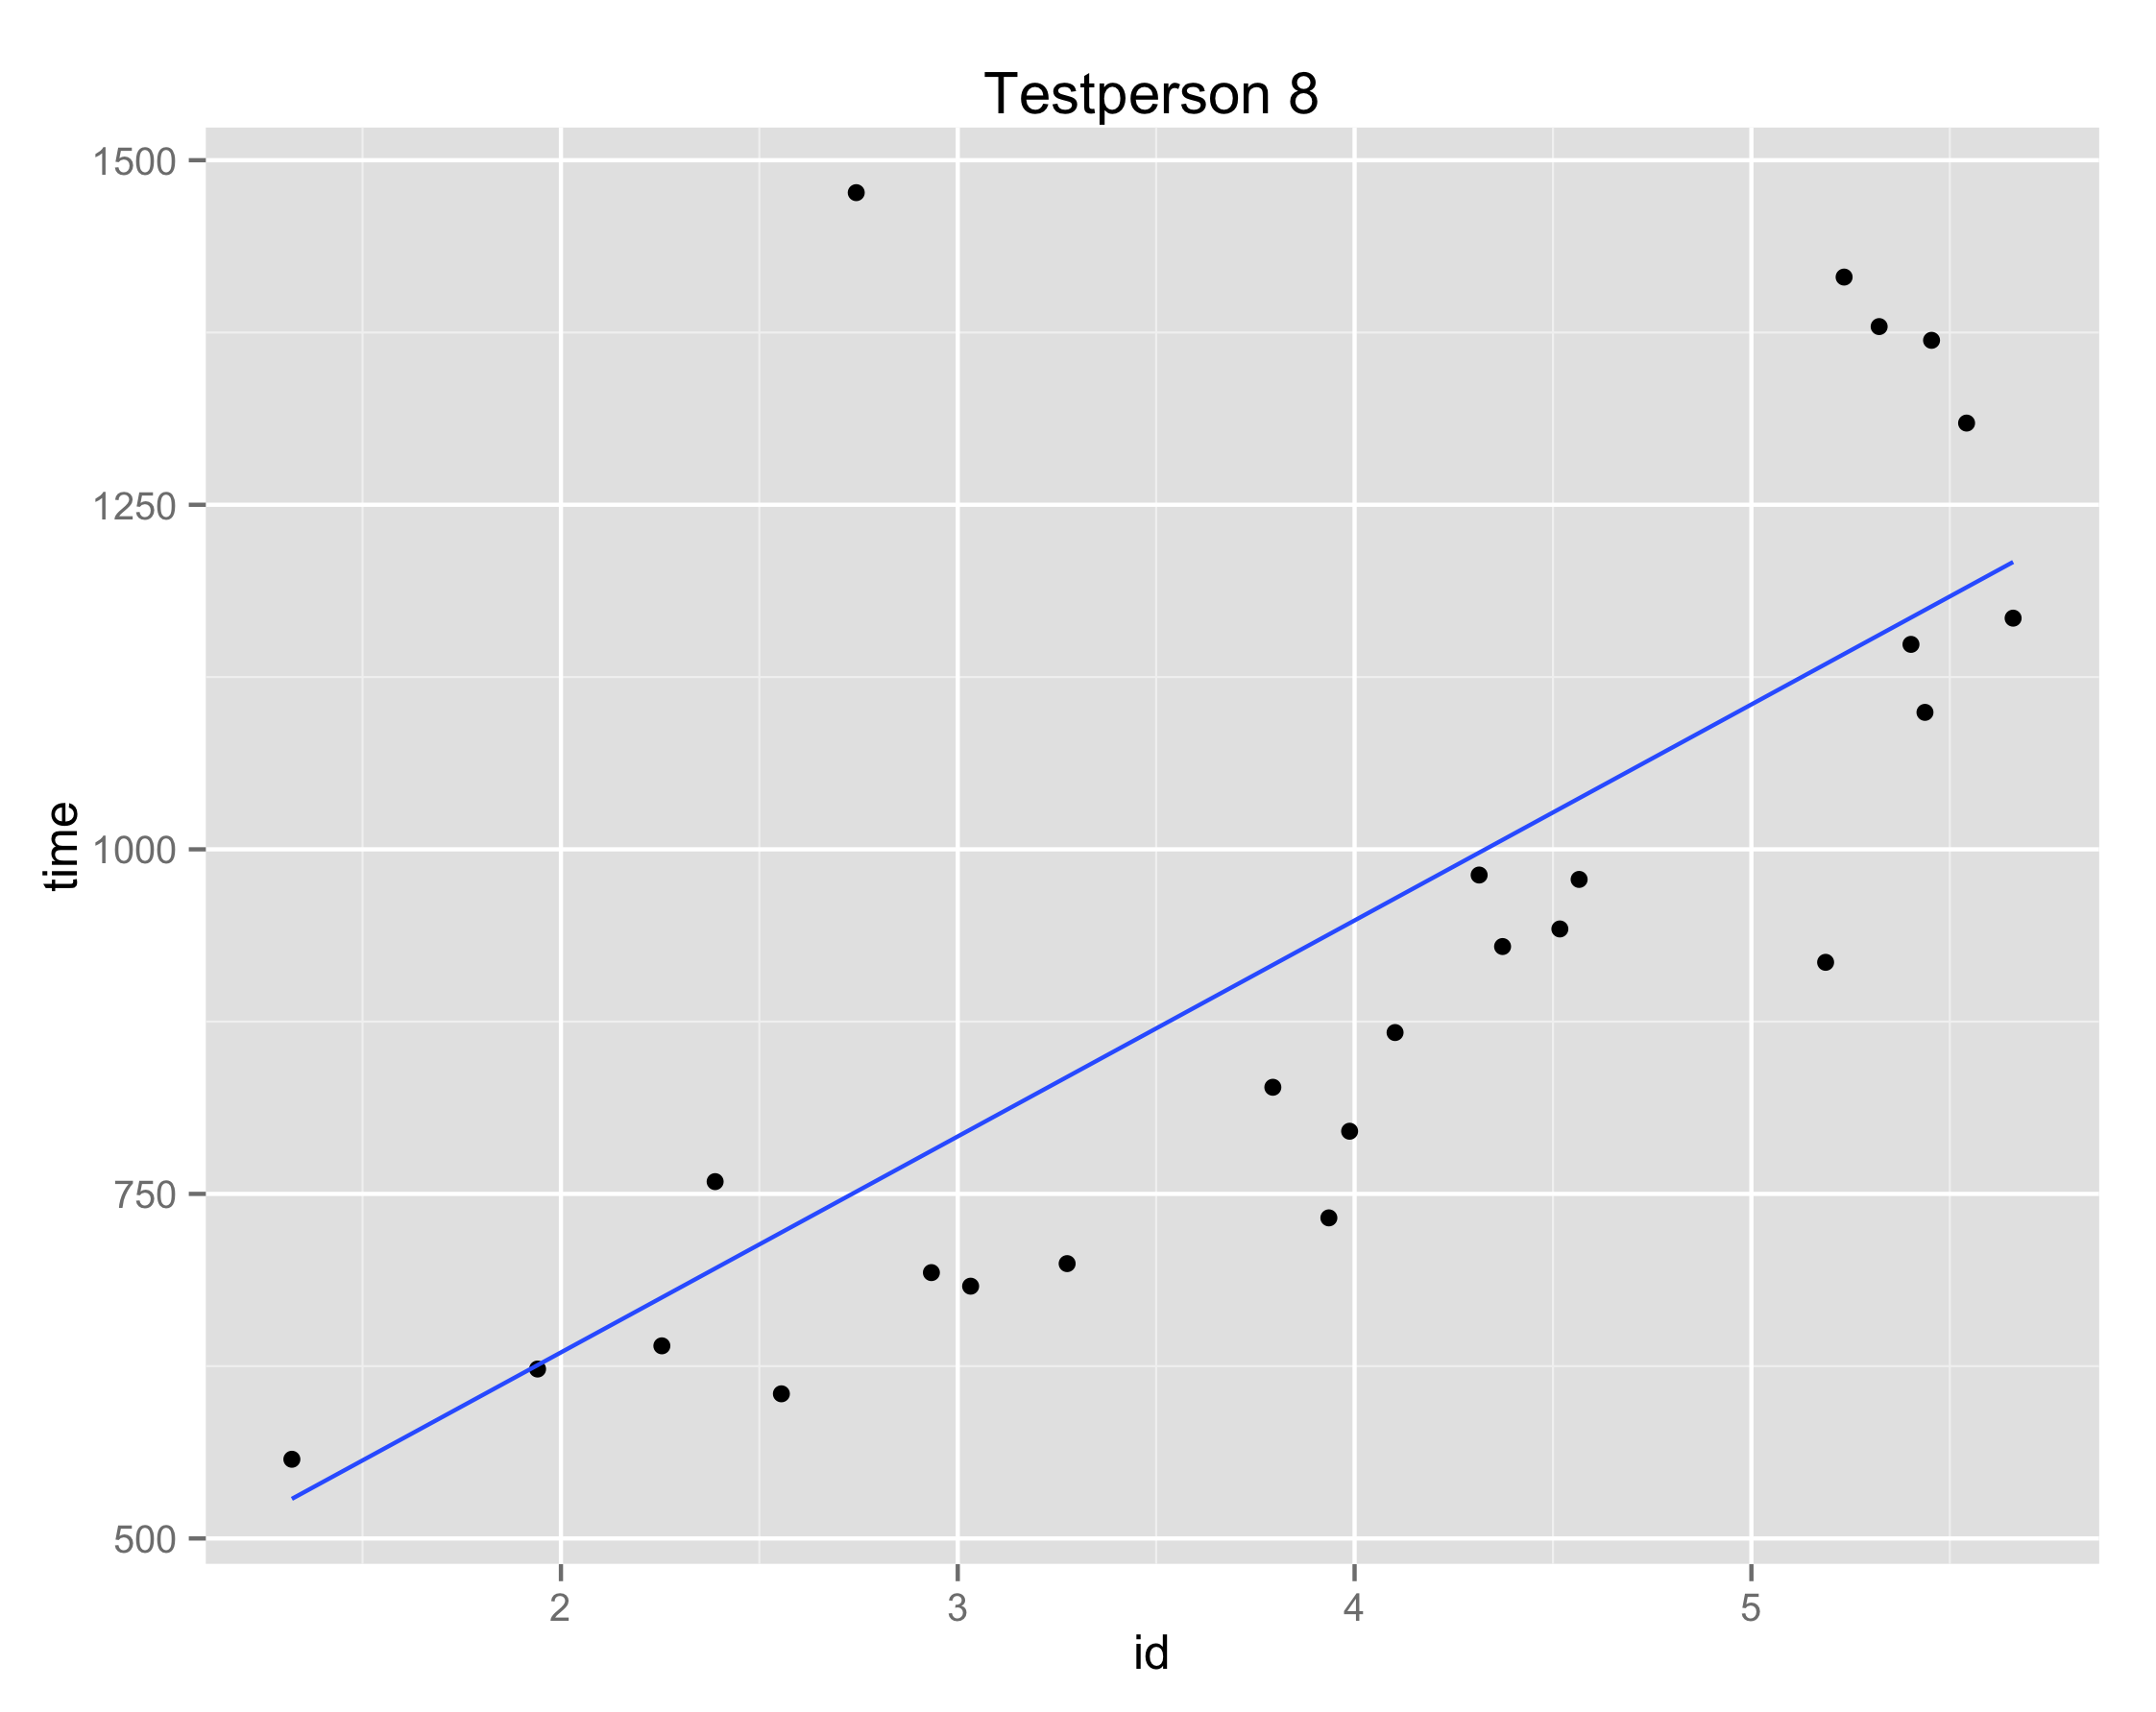
\includegraphics[width=\textwidth]{images/plots/plot_model_test_1}
		\captionof{figure}{Testdeltager 1 med tiden ud af $y$-aksen og $ID$ på $x$-aksen}
		\label{fig:testdeltager1}
	\end{minipage}
	\begin{minipage}[b]{0.50\linewidth}
		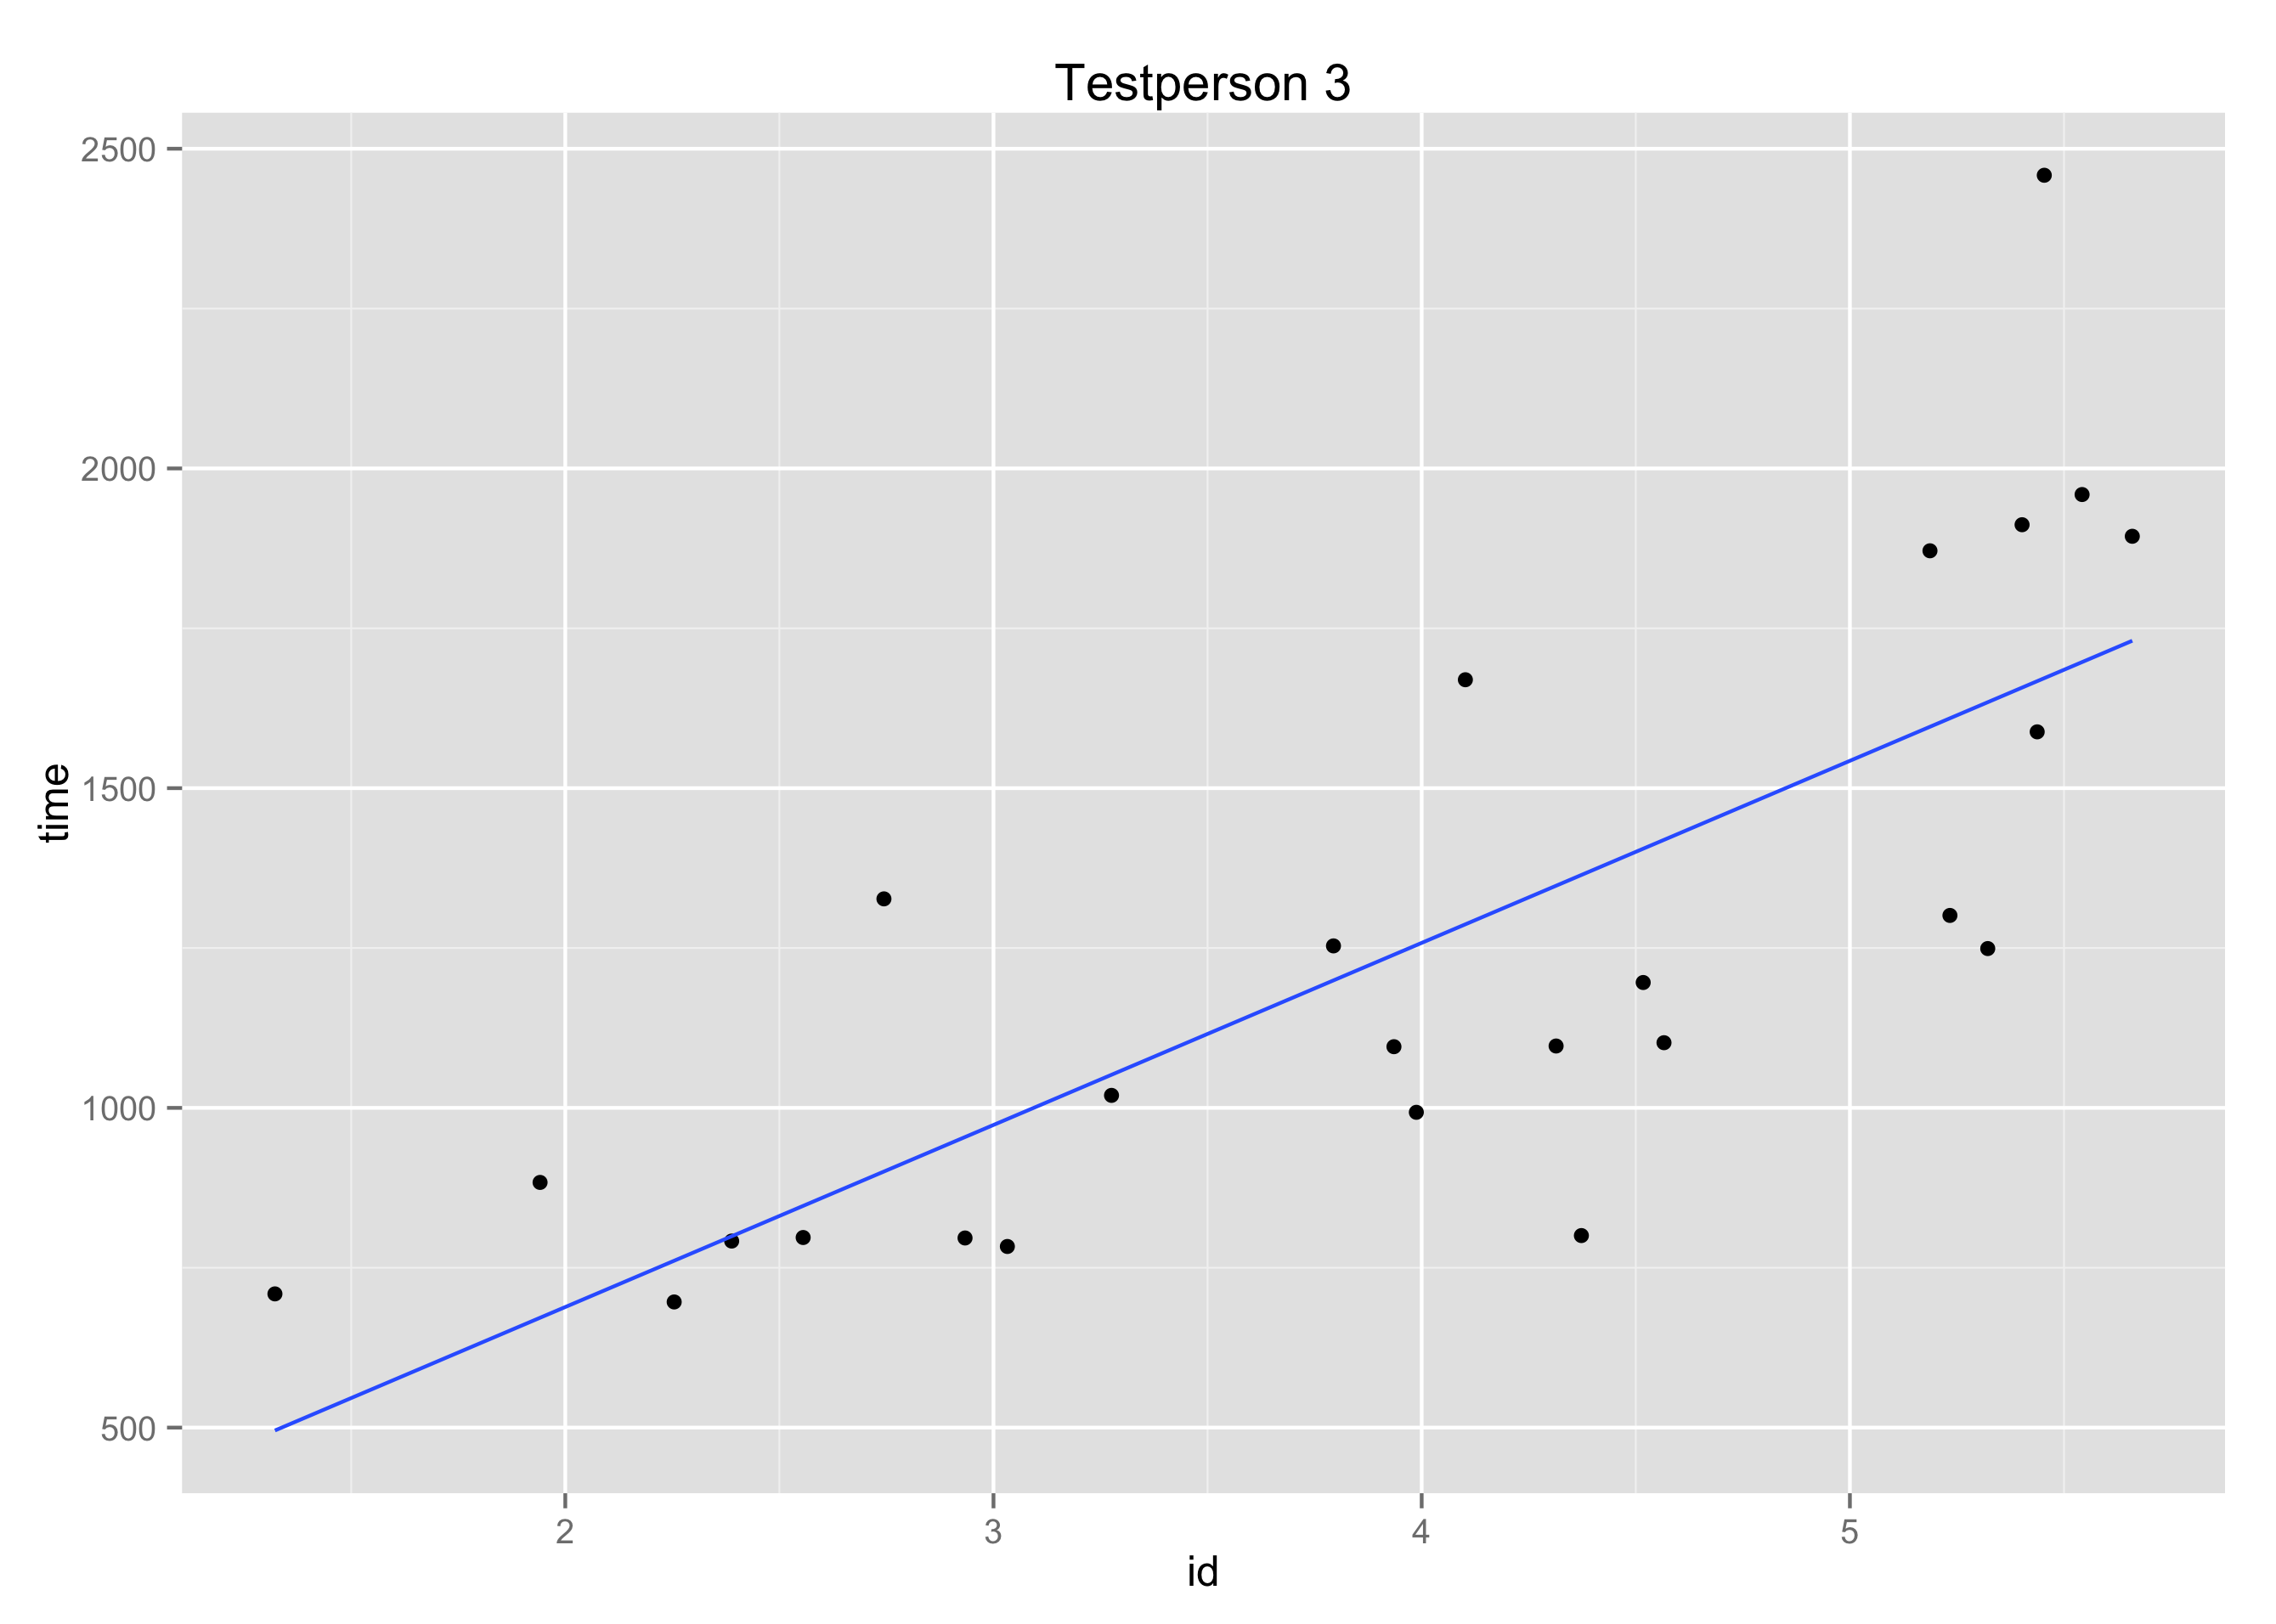
\includegraphics[width=\textwidth]{images/plots/plot_model_test_2}
		\captionof{figure}{Testdeltager 3 med tiden ud af $y$-aksen og $ID$ på $x$-aksen}
		\label{fig:testdeltager3}
	\end{minipage}
\end{minipage}

\newpage
På baggrund af de affine linjers overenstemmelse med størstedelen af datapunkterne fra det kontrollerede eksperiment har vi konkluderet, at det tilsvarende vil gøre sig gældende for vores ukontrollerede data, og derved godt kan danne grundlag for en analyse af de fire formuleringer af Fitts' lov. Vores analyse vil basere sig på et filtreret datasæt ved den oven nævnte $\sigma$ metode, så eventuelle perifære data ikke medtages.

\begin{minipage}{\linewidth}
	\begin{minipage}[b]{.50\linewidth}
		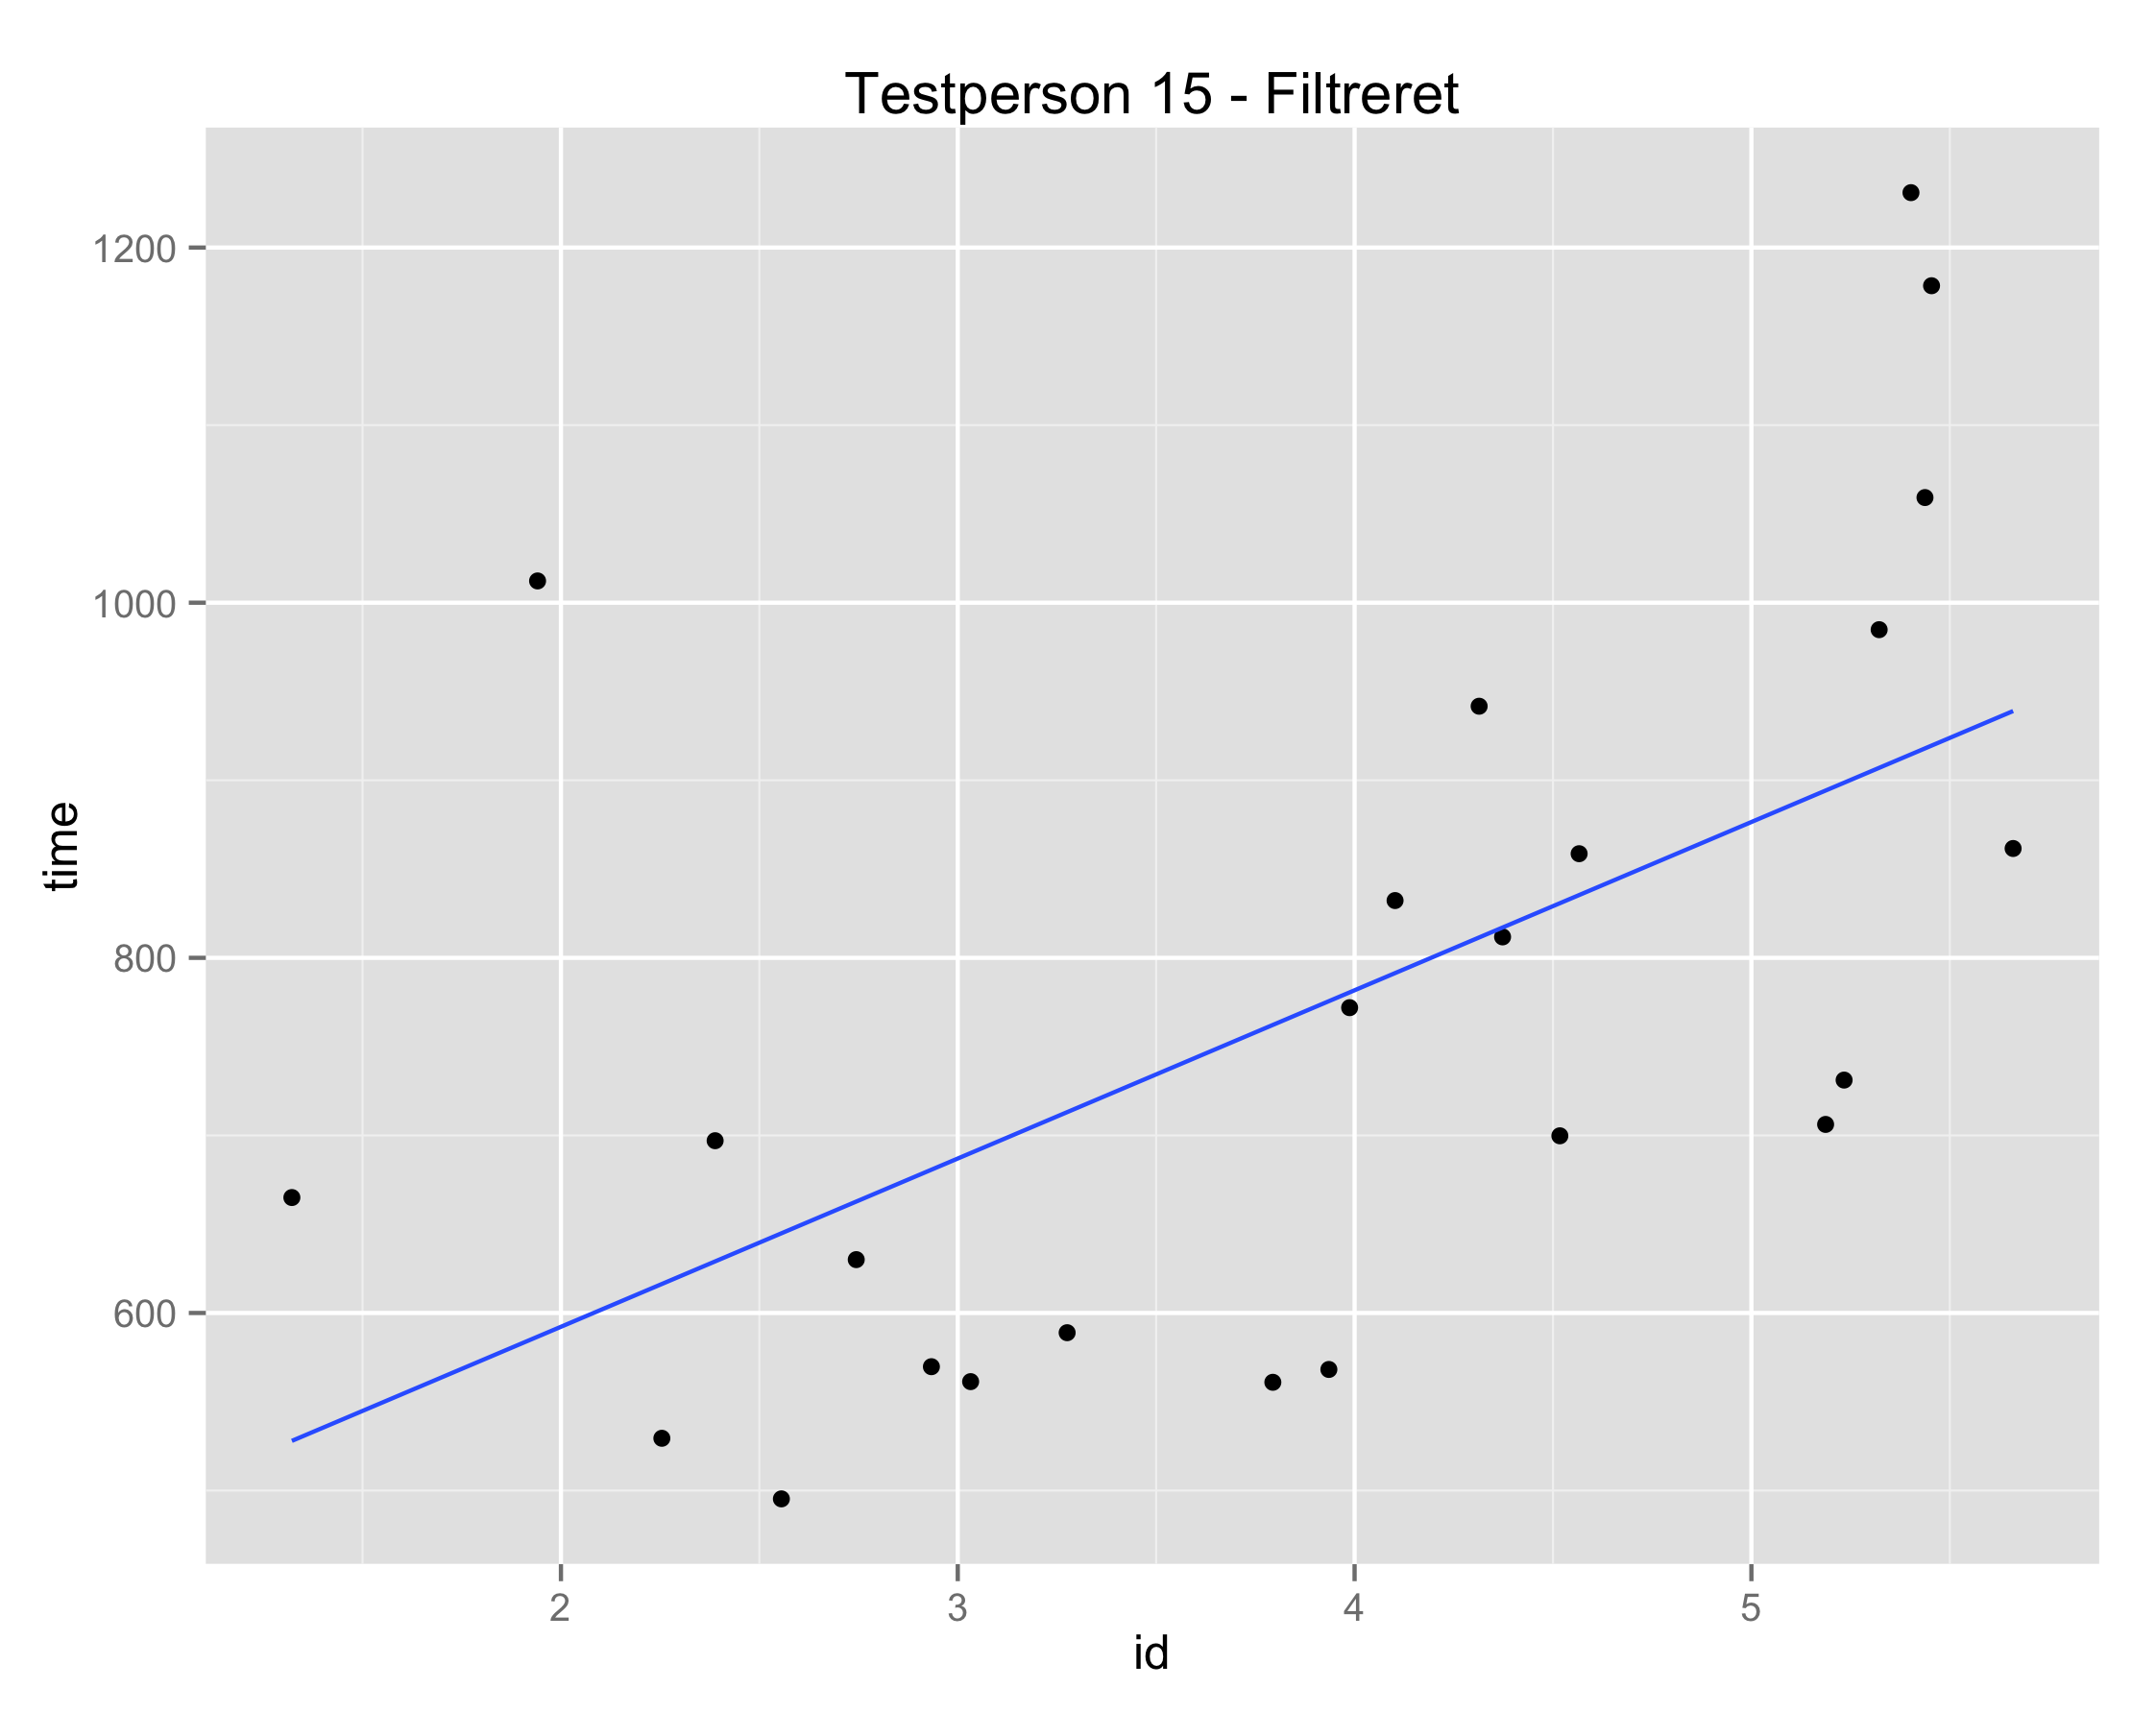
\includegraphics[width=\textwidth]{images/plots/plot_model_test_comparison_filtered}
		\captionof{figure}{Testdeltager 7 med filtreret datasæt}
		\label{fig:testdeltager7filter}
	\end{minipage}
	\begin{minipage}[b]{0.50\linewidth}
		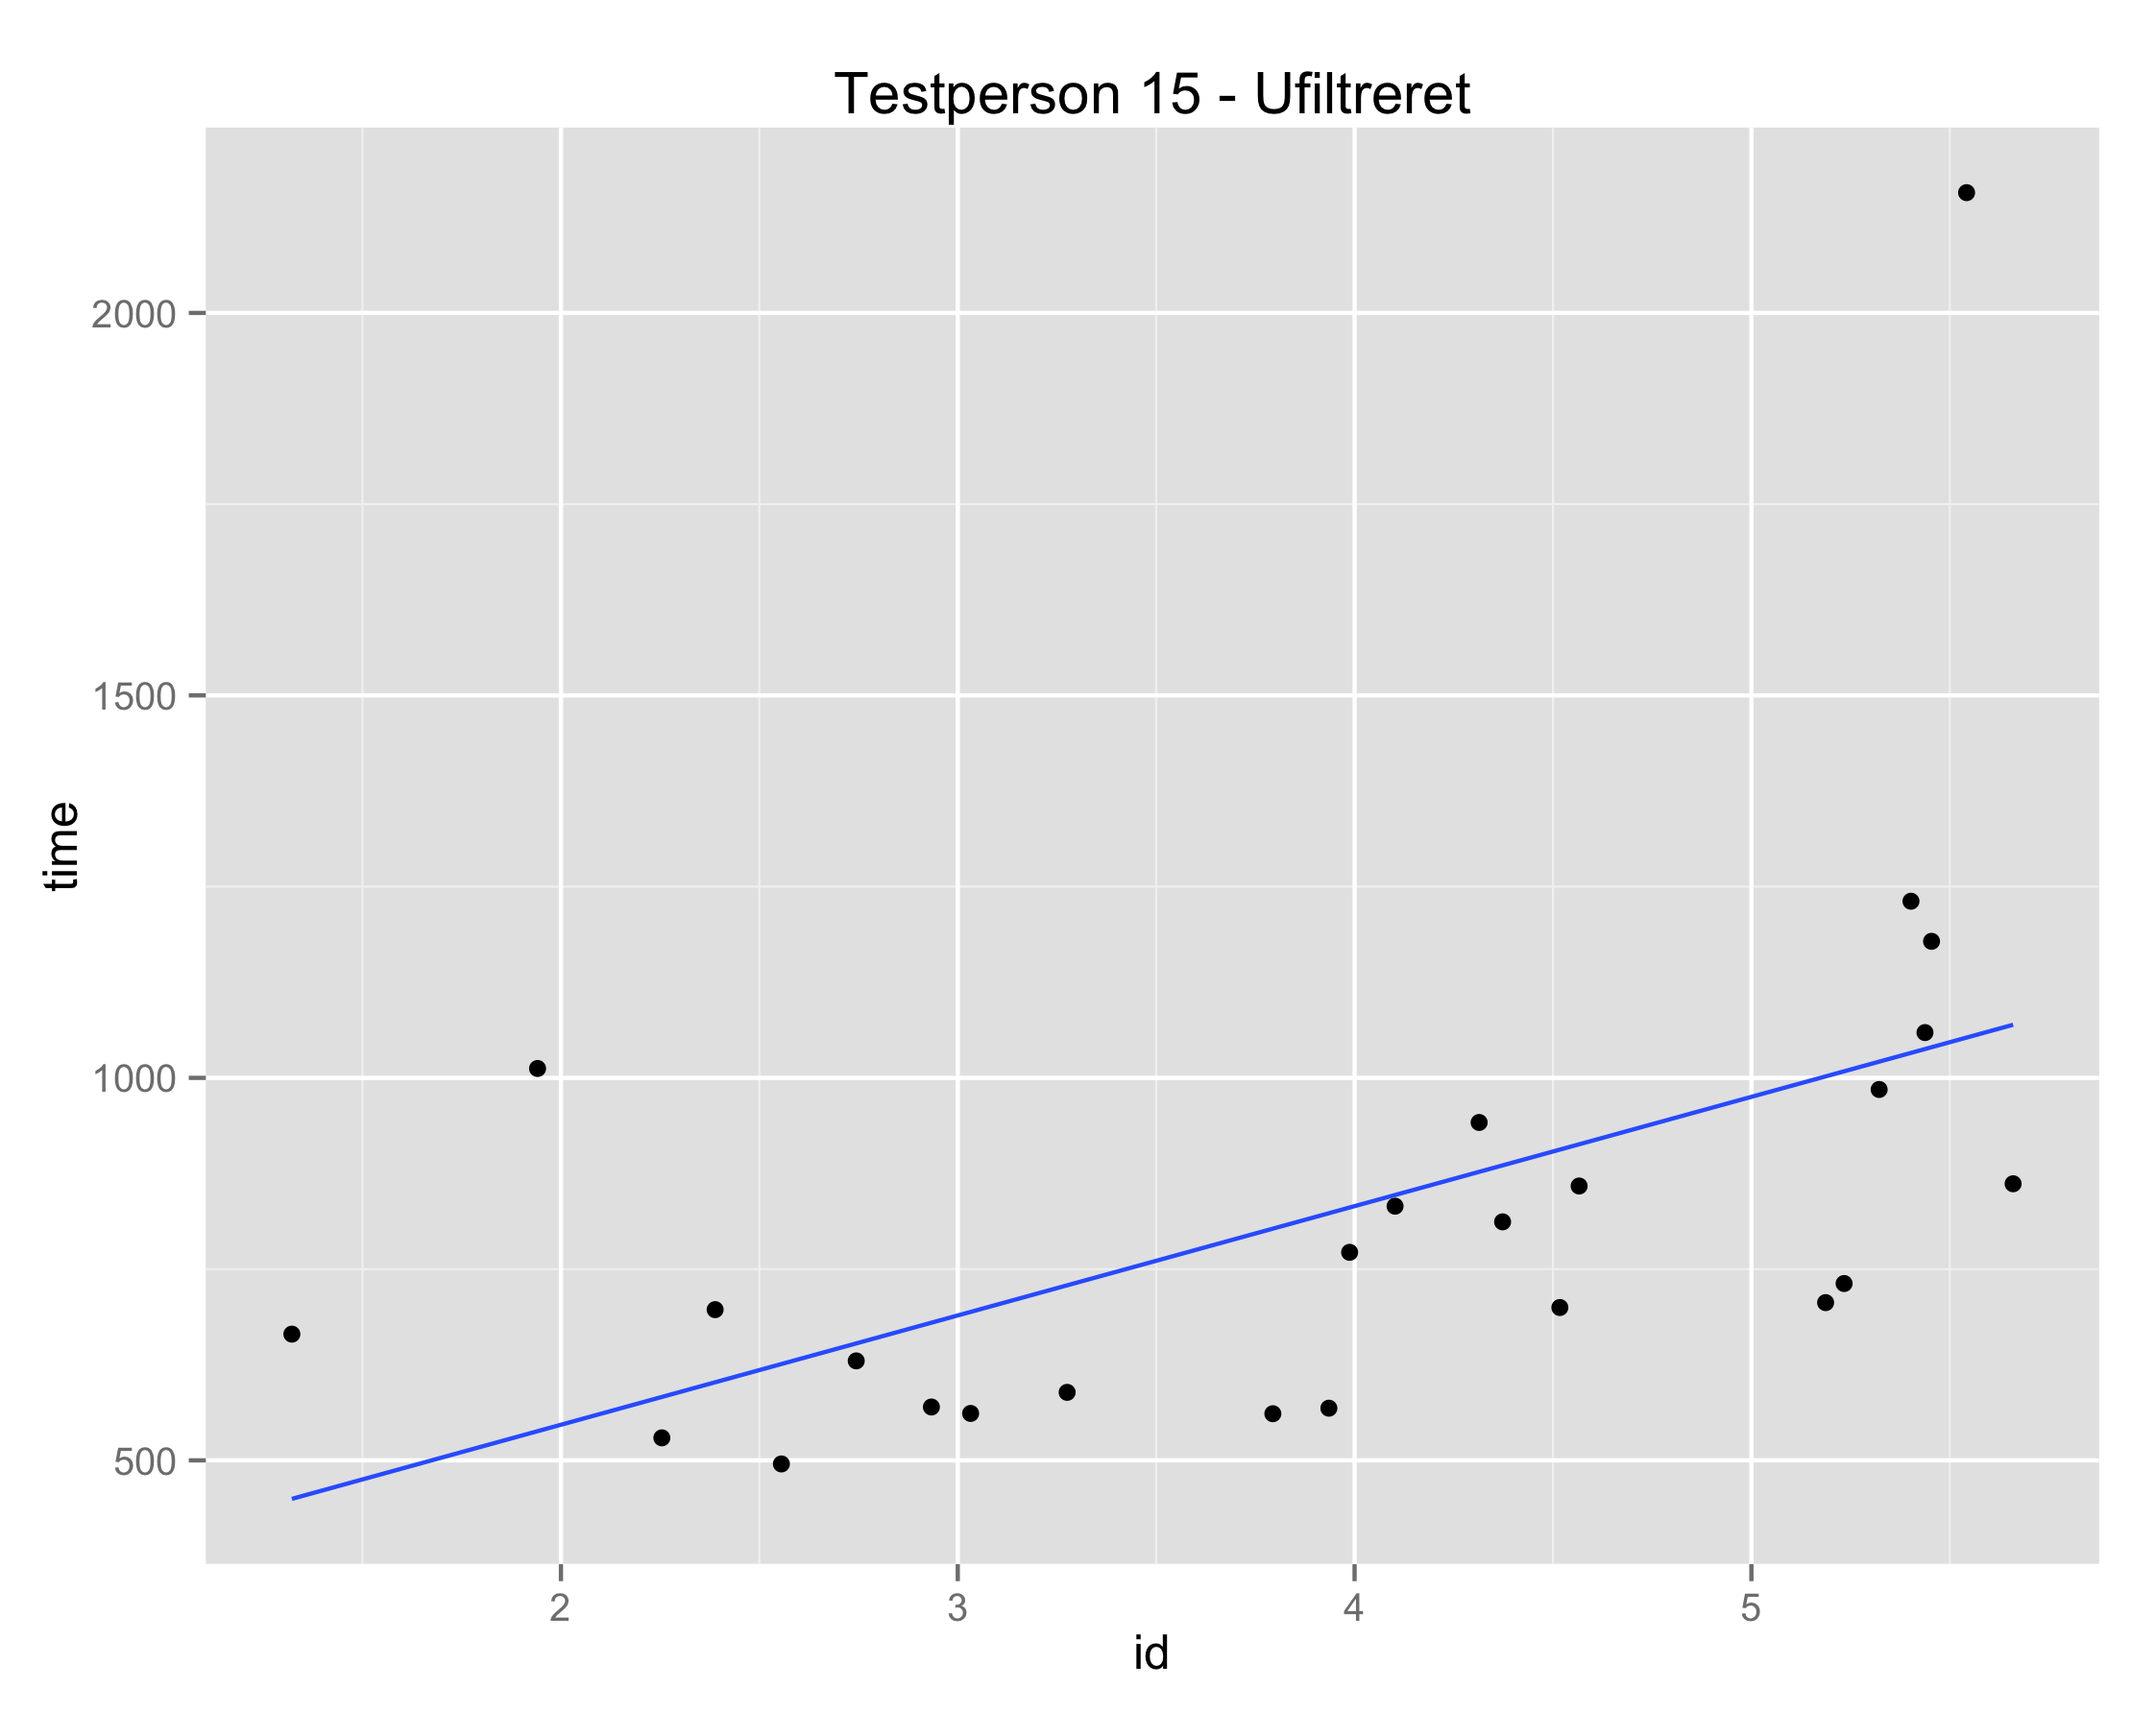
\includegraphics[width=\textwidth]{images/plots/plot_model_test_comparison_unfiltered}
		\captionof{figure}{Testdeltager 7 uden nogen filtrering}
		\label{fig:testdeltager7unfilter}
	\end{minipage}
\end{minipage}

\addcontentsline{toc}{section}{Modelanalyse af bevægelsesbaner}
\section*{Modelanalyse af bevægelsesbaner}
Vores modelanalyse af bevægelsesbaner tager udgangspunkt i AIC-modellen og de bevægelsesbaner der er indsamlet ved crowdsourcingdeltagernes udførsel af opgaverne.

Hver af de fire formuleringer af Fitts lov har vi tilpasset til vores data fra de 264 testdeltageres pegeopgaver ved lineær regression ved R's $lm()$ funktion. Til hver af modellerne har vi gjort brug af formuleringernes respektive $ID$ som $x$-koordinat og tiden, $t$, det tog testdeltageren at løse en pågældende pegeopgave som $y$-koordinat. De fire matematiske modeller med de tilpassede konstanter er vist nedenfor.
\begin{align*}
\text{Fitts': } &T = 392.29 + 149.42\cdot \log_2\left(\frac{2A}{W}\right)\\
\text{Welford's: } &T =  299.73\cdot \log_2\left(\frac{A+\frac{1}{2}W}{W}\right)\\
\text{Mackenzie's: } &T = 418.58 + 176.87\cdot \log_2\left(\frac{A+W}{W}\right)\\
\text{Meyer's: } &T = 504.48 + 157.13 \cdot \sqrt{\frac{A}{W}}
\end{align*}

Bemærk at den additive konstant er målt i millisekunder ligesom vores registrerede tider fra datasættet. Ud fra de tre additive konstanter, kan det ses, at testdeltagerne i gennemsnit bruger cirka 450 millisekunder på at opfange opgaven før de bevæger deres pegeenhed. Datapunkterne og de fire affine modeller er plottet og vist i figur \ref{fig:welford_affine_line}, \ref{fig:fitt_affine_line}, \ref{fig:meyer_affine_line} og \ref{fig:mackenzie_affine_line}. Bemærk, hvordan datapunkterne danner 25 vertikale 'søjler', én for hvert af vores pegeopgavers $ID$.

Det er de fire matematiske modeller som vores pegeopgaveanalyse vil tage udgangspunkt i. Ud fra modellerne og figurerne er det dog svært at sige noget om, hvilke af modellerne der klarer sig bedre i at beskrive datapunkterne end resten. Vi vil derfor gøre brug af en AIC sammenligning og underbygge den med en residualanalyse.


\begin{minipage}{\linewidth}
	\begin{minipage}[b]{0.45\linewidth}
		\captionof{figure}{Welford's lineære model med hans $ID$ ud af $x$-aksen og tiden ud af $y$-aksen}
		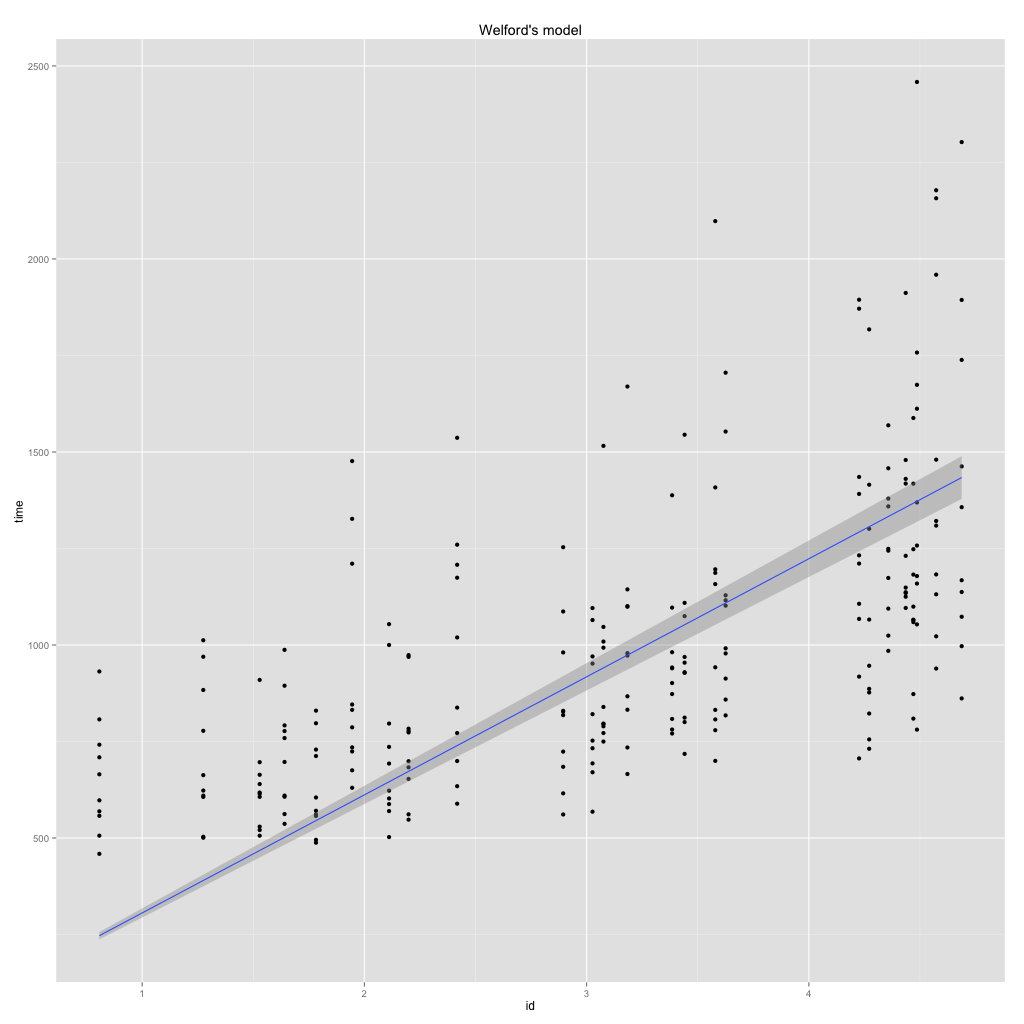
\includegraphics[width=\textwidth]{images/plots/plot_model_welford}
		\label{fig:welford_affine_line}
	\end{minipage}
	\begin{minipage}[b]{0.1\linewidth}
	~
	\end{minipage}
	\begin{minipage}[b]{0.45\linewidth}
		\captionof{figure}{Fitts' affine model med hans $ID$ ud af $x$-aksen og tiden ud af $y$-aksen}
		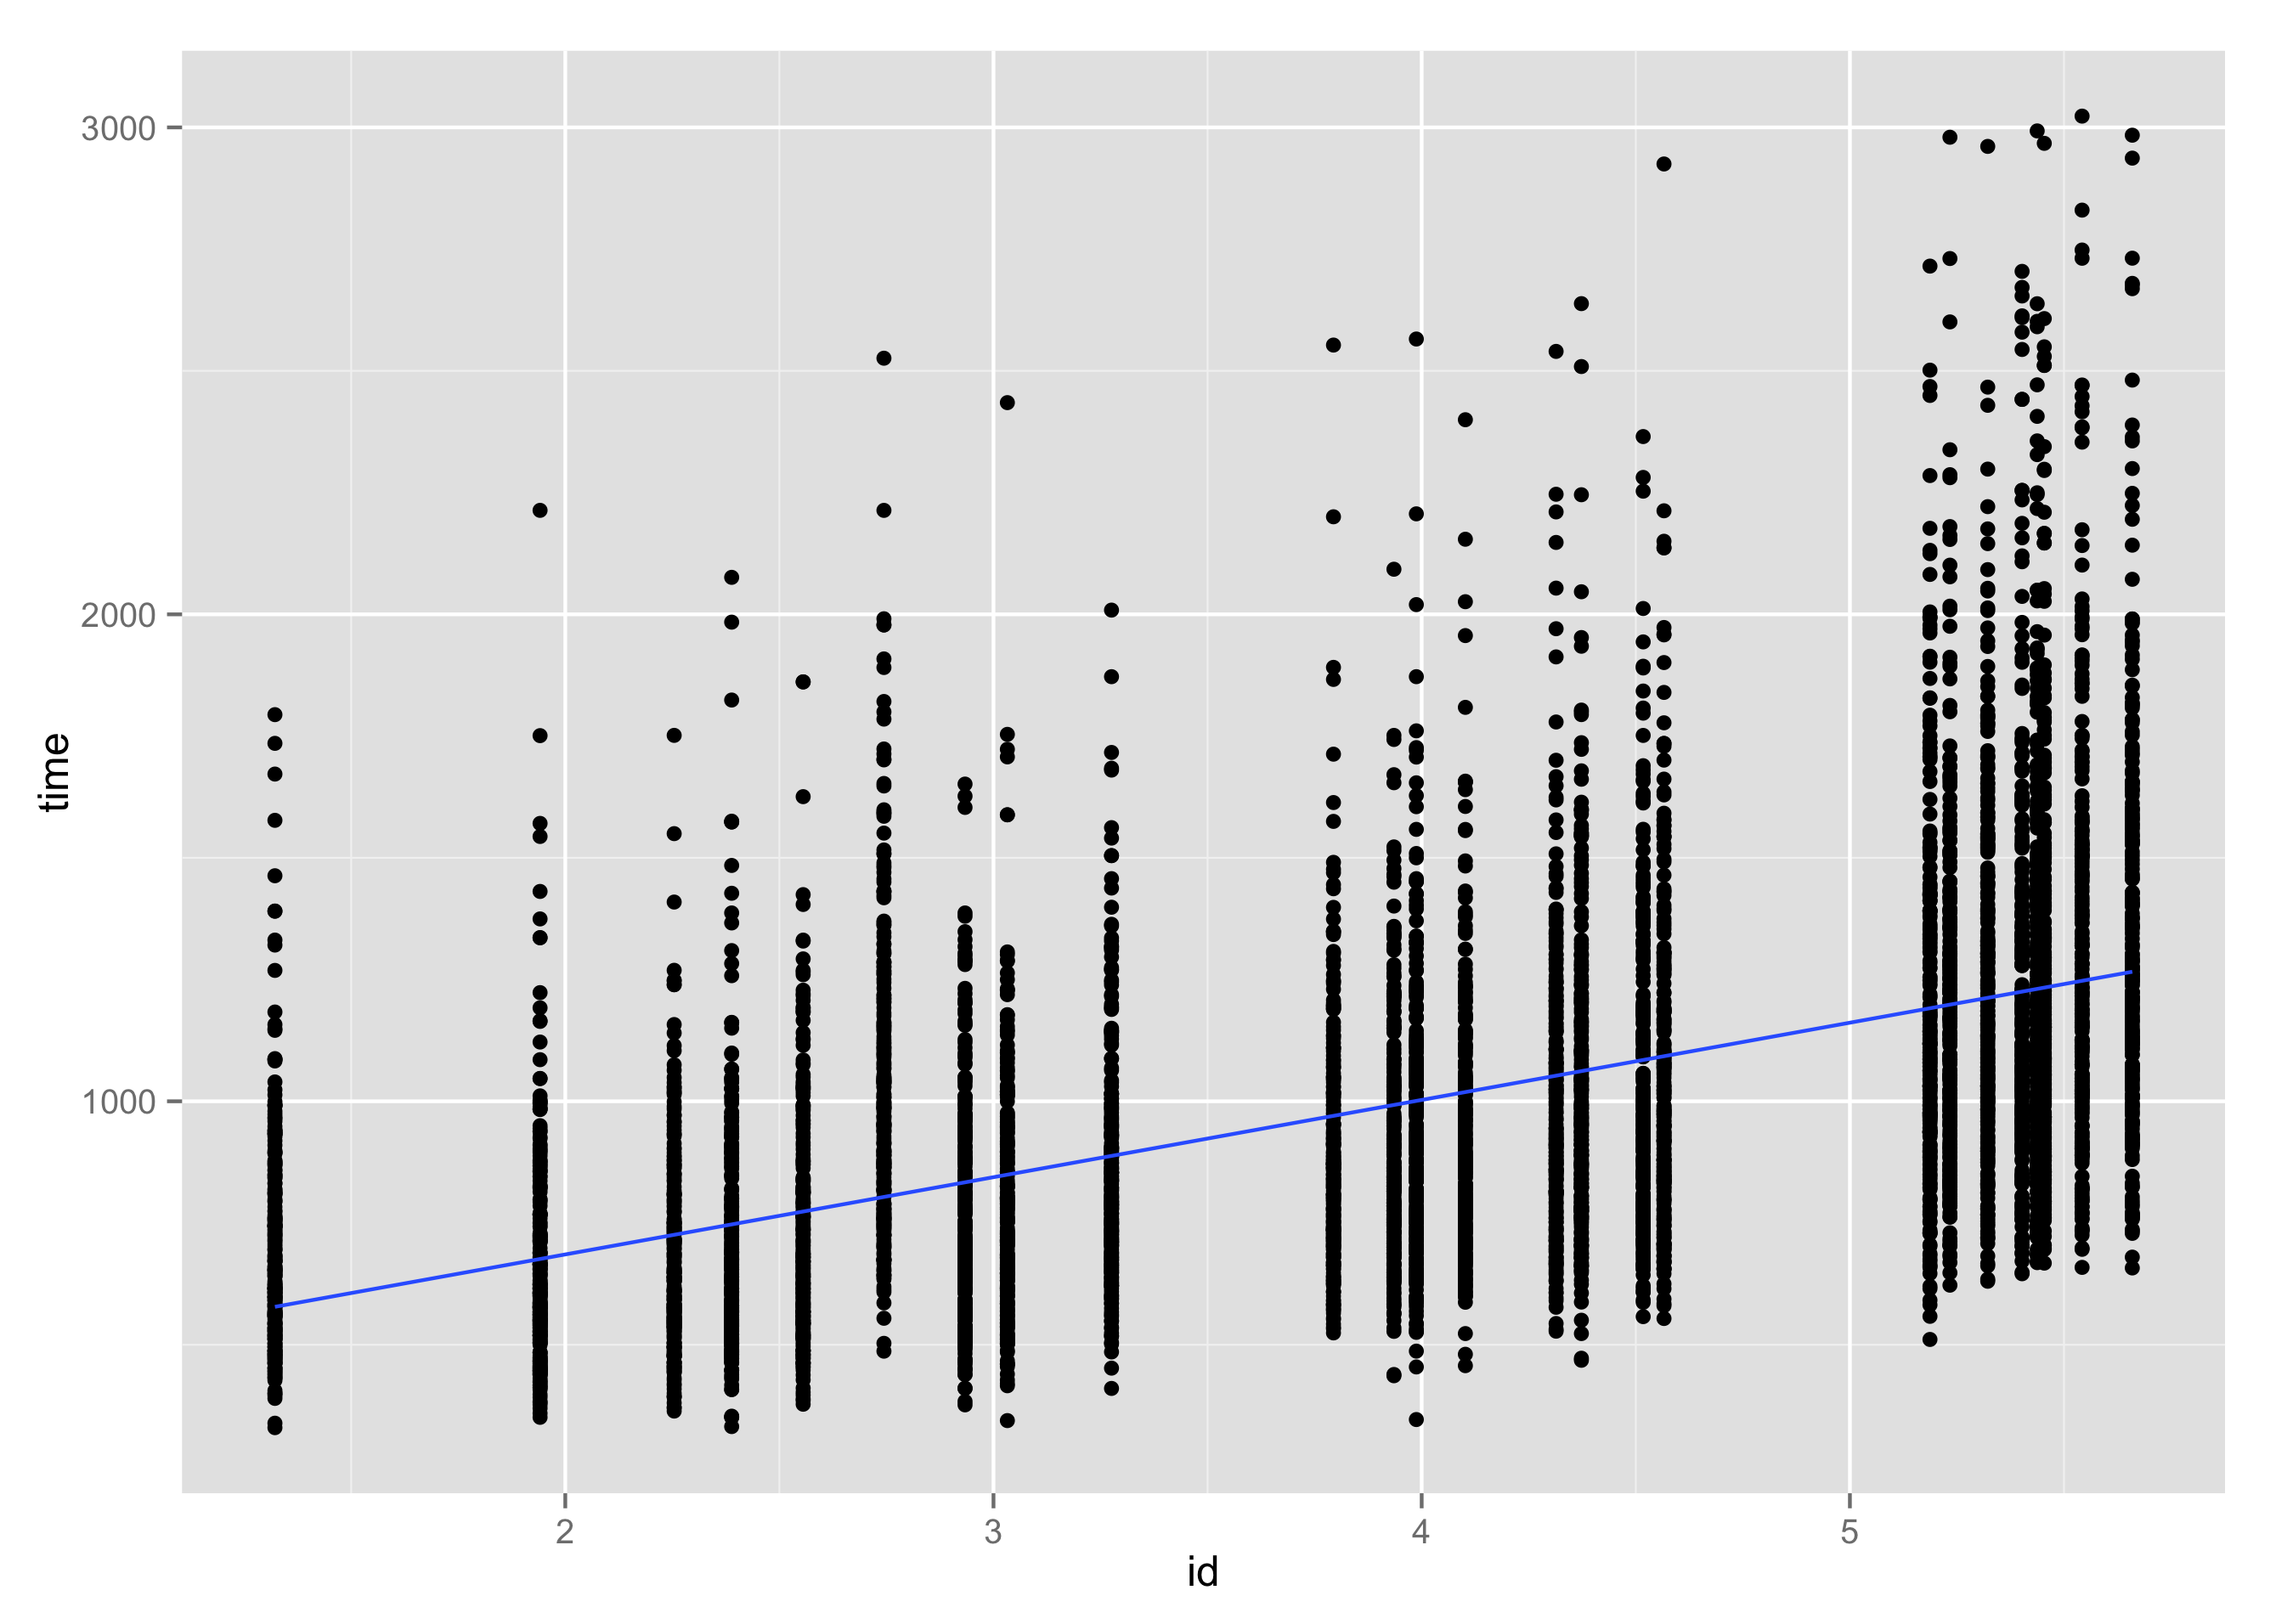
\includegraphics[width=\textwidth]{images/plots/plot_model_fitt}
		\label{fig:fitt_affine_line}
	\end{minipage}
	\begin{minipage}[b]{0.45\linewidth}
		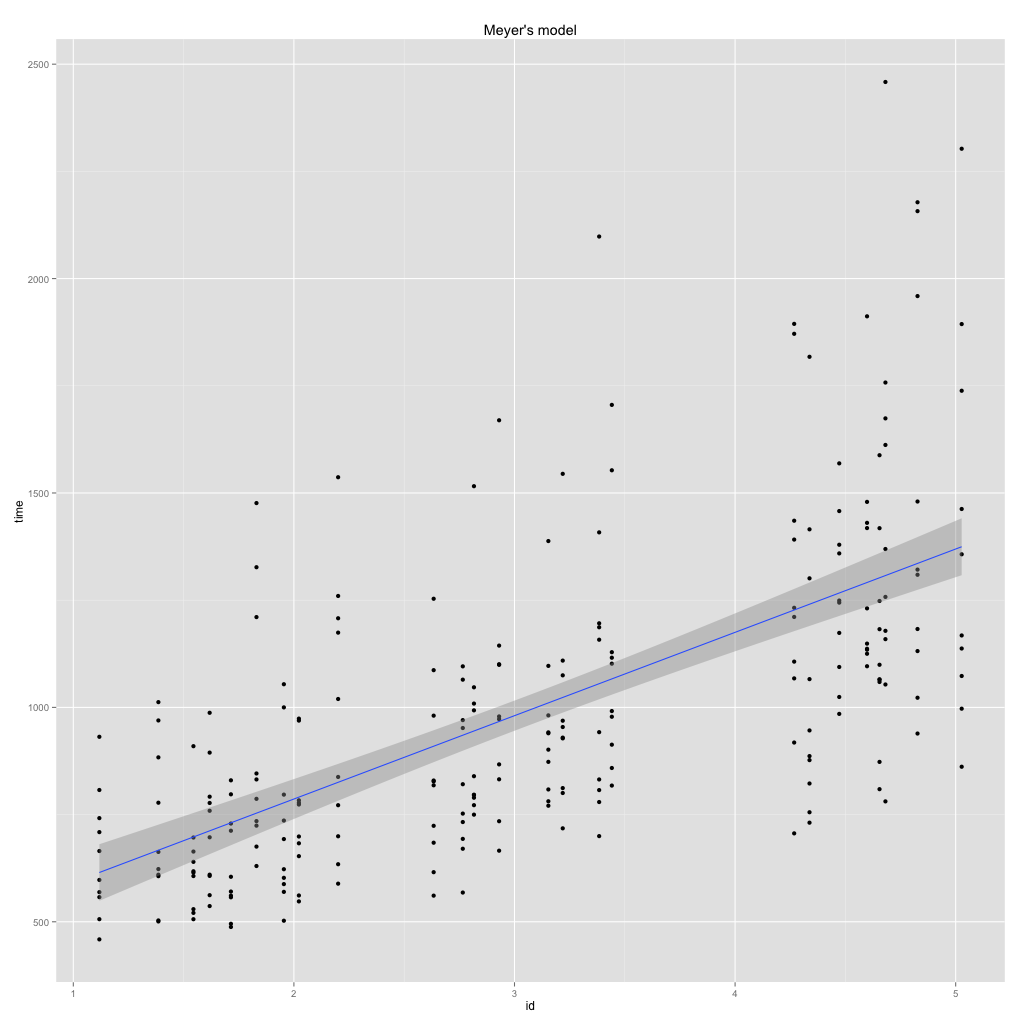
\includegraphics[width=\textwidth]{images/plots/plot_model_meyer}
		\captionof{figure}{Meyer's affine model med hans $ID$ ud af $x$-aksen og tiden ud af $y$-aksen}
		\label{fig:meyer_affine_line}
	\end{minipage}
	\begin{minipage}[b]{0.1\linewidth}
	~
	\end{minipage}
	\begin{minipage}[b]{0.45\linewidth}
		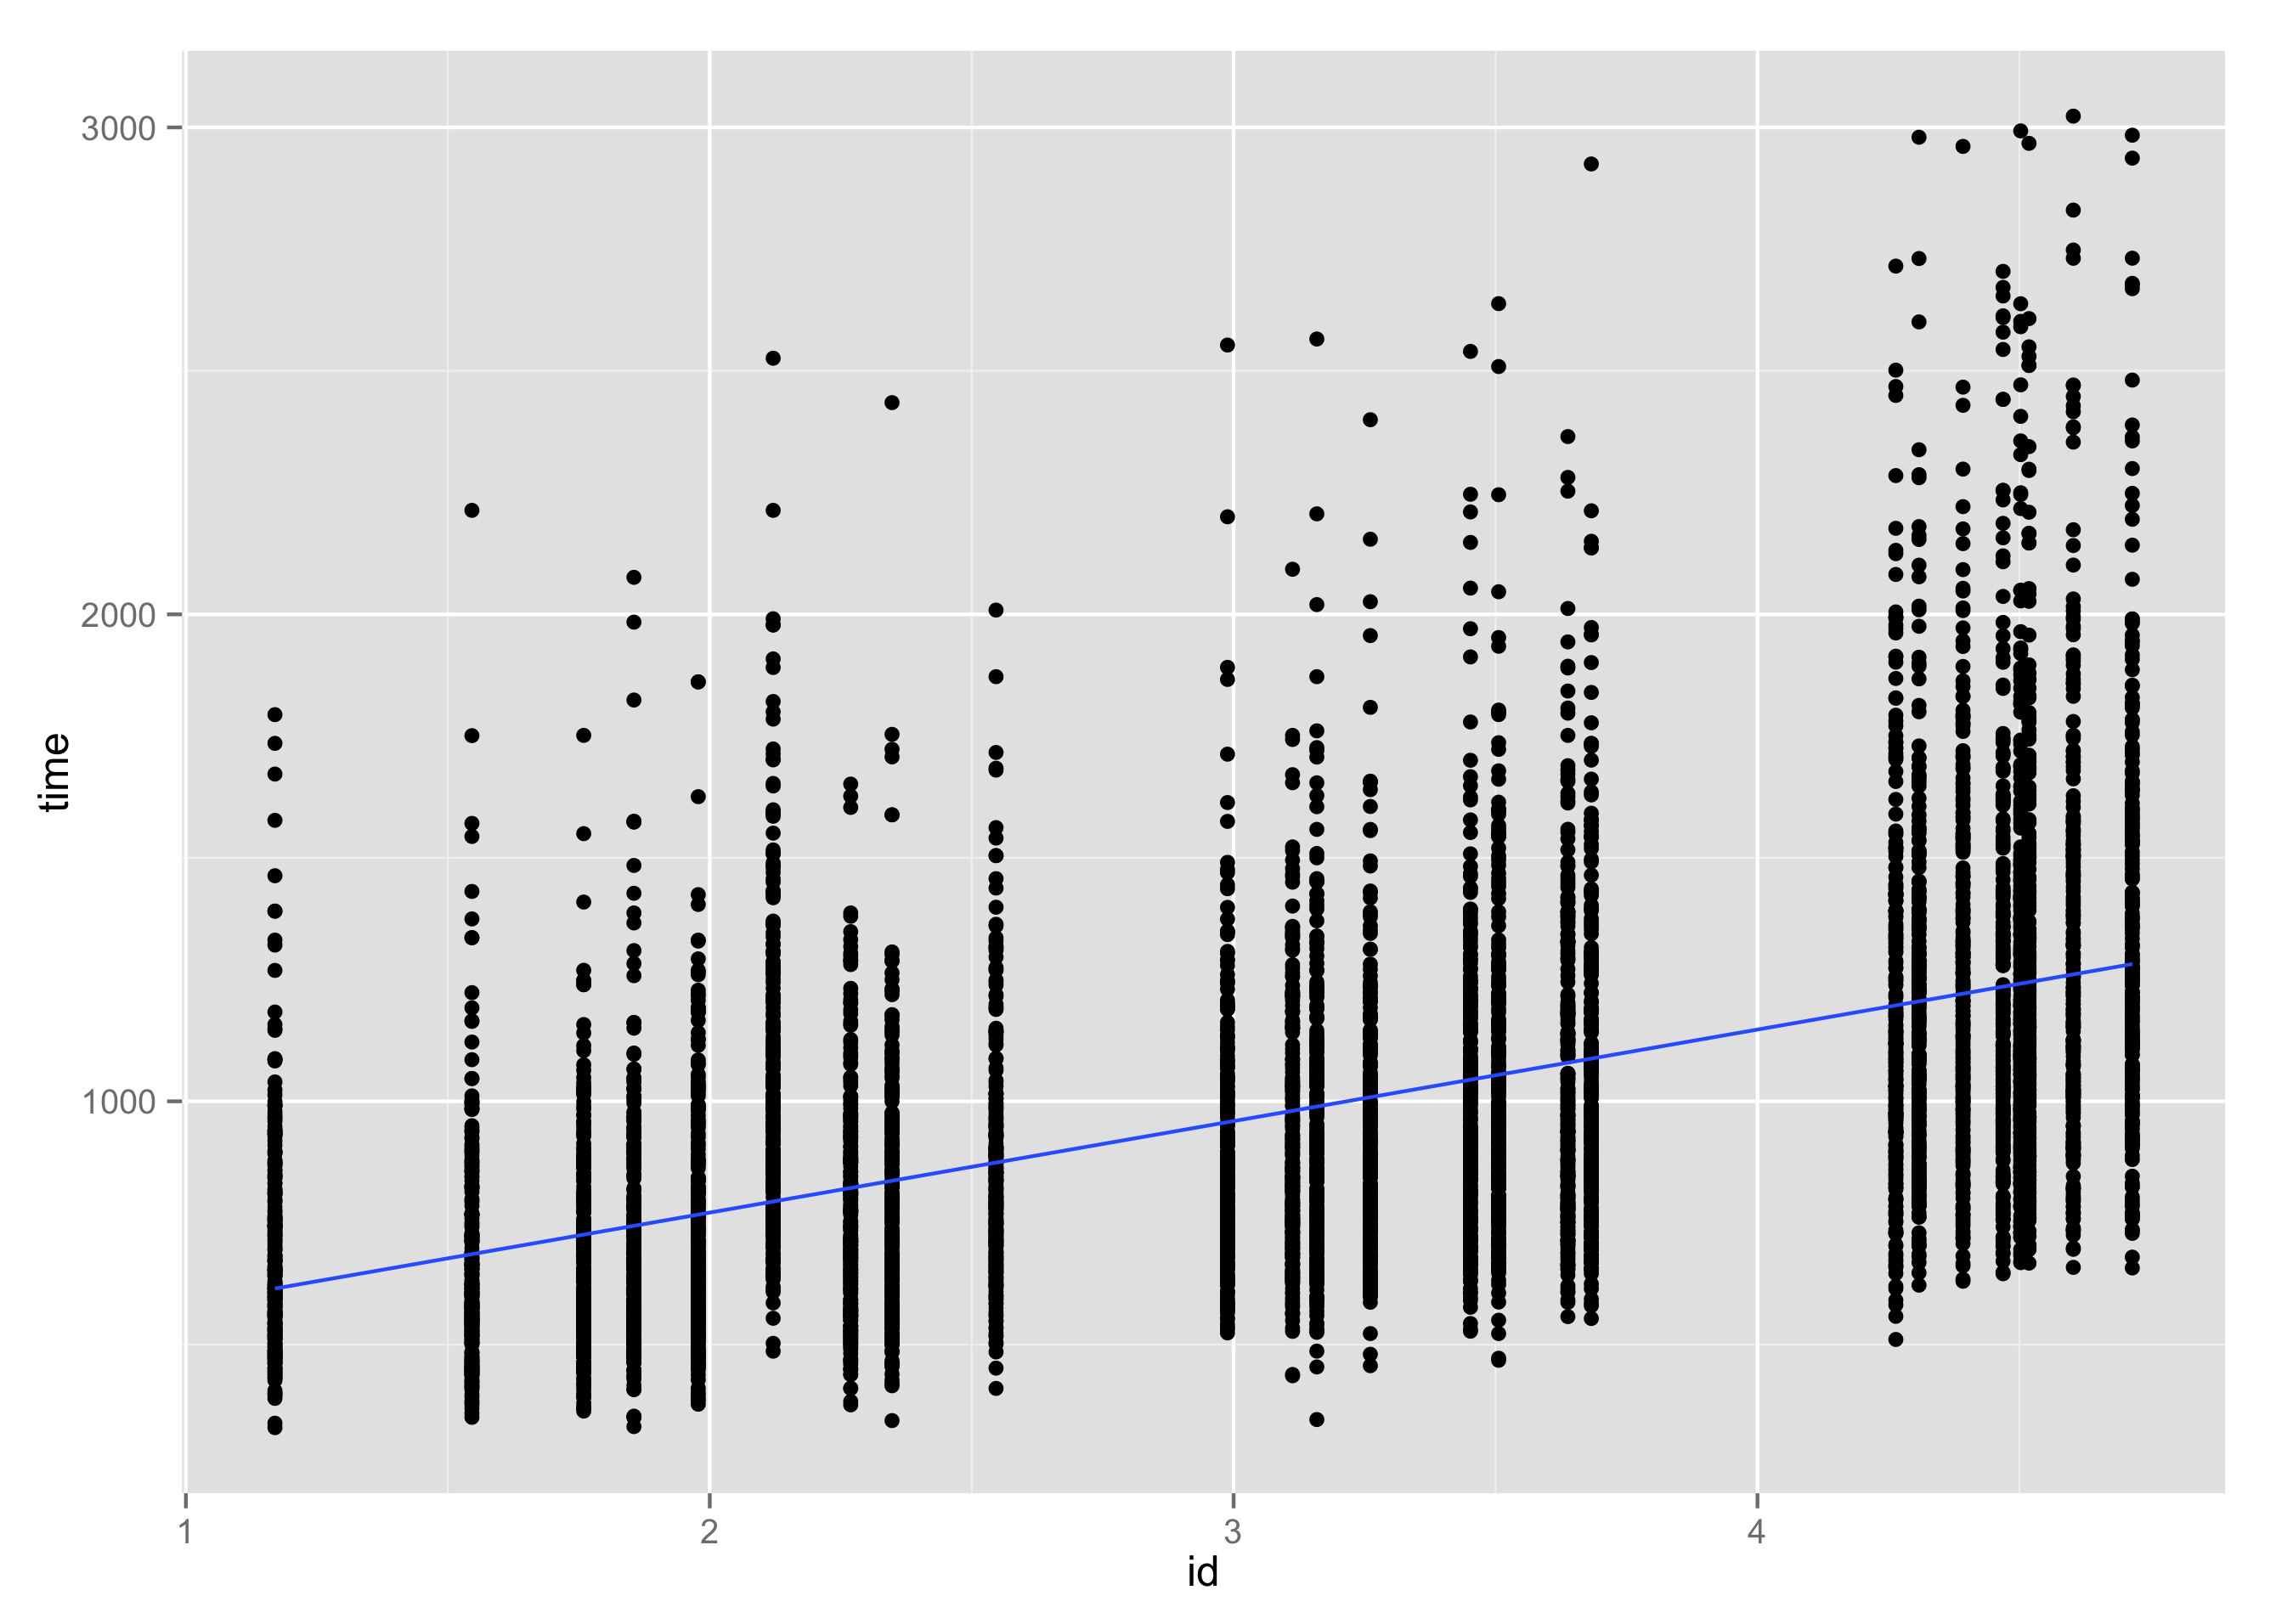
\includegraphics[width=\textwidth]{images/plots/plot_model_mackenzie}
		\captionof{figure}{Mackenzie's affine model med hans $ID$ ud af $x$-aksen og tiden ud af $y$-aksen}
		\label{fig:mackenzie_affine_line}
	\end{minipage}
\end{minipage}

\addcontentsline{toc}{subsection}{AIC-analyse}
\subsection*{AIC-analyse}
AIC anslår kvaliteten af hver model, relativt til hver af de andre modeller. Hvilket vil sige at AIC ikke kan sige noget om kvaliteten af en model I absolut forstand, og derfor ikke kan vurdere hvor godt en model passer på dataen - kun den relative kvalitet af hver model.

Tabel \ref{tab:table_analysis_aic1} viser AIC-værdierne, og den relative forskel i mellem dem, for de fire modeller. Eftersom den absolute AIC-værdi ikke I sig selv siger noget, kigger vi kun på forskellen mellem dem.

Det ses af tabel \ref{tab:table_analysis_aic1} at vi bruger modellen med den laveste værdi, altså Meyer's, som nulpunkt. Det ses deraf at forskellen mellem de tre modeller med den laveste AIC-værdi (Meyer, MacKenzie, Fitts) ikke er betydelig, I forhold til forskellen mellem disse og Welford's model.

Det vi kan uddrage af denne analyse, er at vi har med nogle meget ensartede modeller at gøre, I forhold til hvordan de passer på dataen, dog med undtagelse af Welford's model.

\begin{table}[h]
\centering
\begin{tabular}{lll}
Model 	  & AIC-værdi & Forskel\\\hline
Meyer 	  & 92728.38 & 0 \\
Mackenzie & 92763.02 & 34.64 \\
Fitts 	  & 92804.17 & 75.79 \\
Welford   & 94510.34 & 1781.96
\end{tabular}
\caption{AIC værdier og indbyrdes forskel med udgangspunkt i Meyers som nulpunkt}
\label{tab:table_analysis_aic1}
\end{table}

\addcontentsline{toc}{subsection}{Residualanalyse}
\subsection*{Residualanalyse}
For at få en ekstra vurdering af præcisionen af modellerne, har vi valgt at lave en residualanalyse ved hjælp af residualplots. Residualerne I modellerne er variationen i $ID$ som modellerne ikke når at opfange, og de kan derved sige noget om hvor præcis modellerne er i forhold til den data vi har indsamlet.\\
På figur \ref{fig:plot_residual_fitt}, \ref{fig:plot_residual_welford}. \ref{fig:plot_residual_mackenzie} og \ref{fig:plot_residual_meyer} ses alle fire modellers residualplot, med en rød linje defineret af en smoothing-funktion. Smoothing-funktionen er tilføjet som et visuelt hjælpemiddel der tydeligt kan vise hvordan residualerne fordeler sig omkring x-aksen. Jo mere centreret de er om aksen, og jo mere linære de er i forhold til aksen, jo bedre er modellen.\\
Når vi kigger på de fire residualplot, så viser de samme resultater som AIC-analysen. Welford's residualplot viser at modellen passer dårlig på den indsamlede data. Fitt's og MacKenzie's ligner hinanden meget, mens Meyer's er den model der giver den bedste fit til den indsamlede data.\\
Det ses af figur \ref{fig:plot_residual_welford} at Welford's især er dårligere ved lavere værdier af $ID$. Grunden til dette skal findes i at Welford's ikke har det additive $a$-led. Som Welford \cite{welford1968} selv forklare, så vil det manglende $a$-led ikke gøre stor forskel ved større værdier af $ID$. Fitt's og MacKenzie's residualer ligner hinanden rigtig meget.

\begin{minipage}{\linewidth}
	\begin{minipage}{.5\linewidth}
		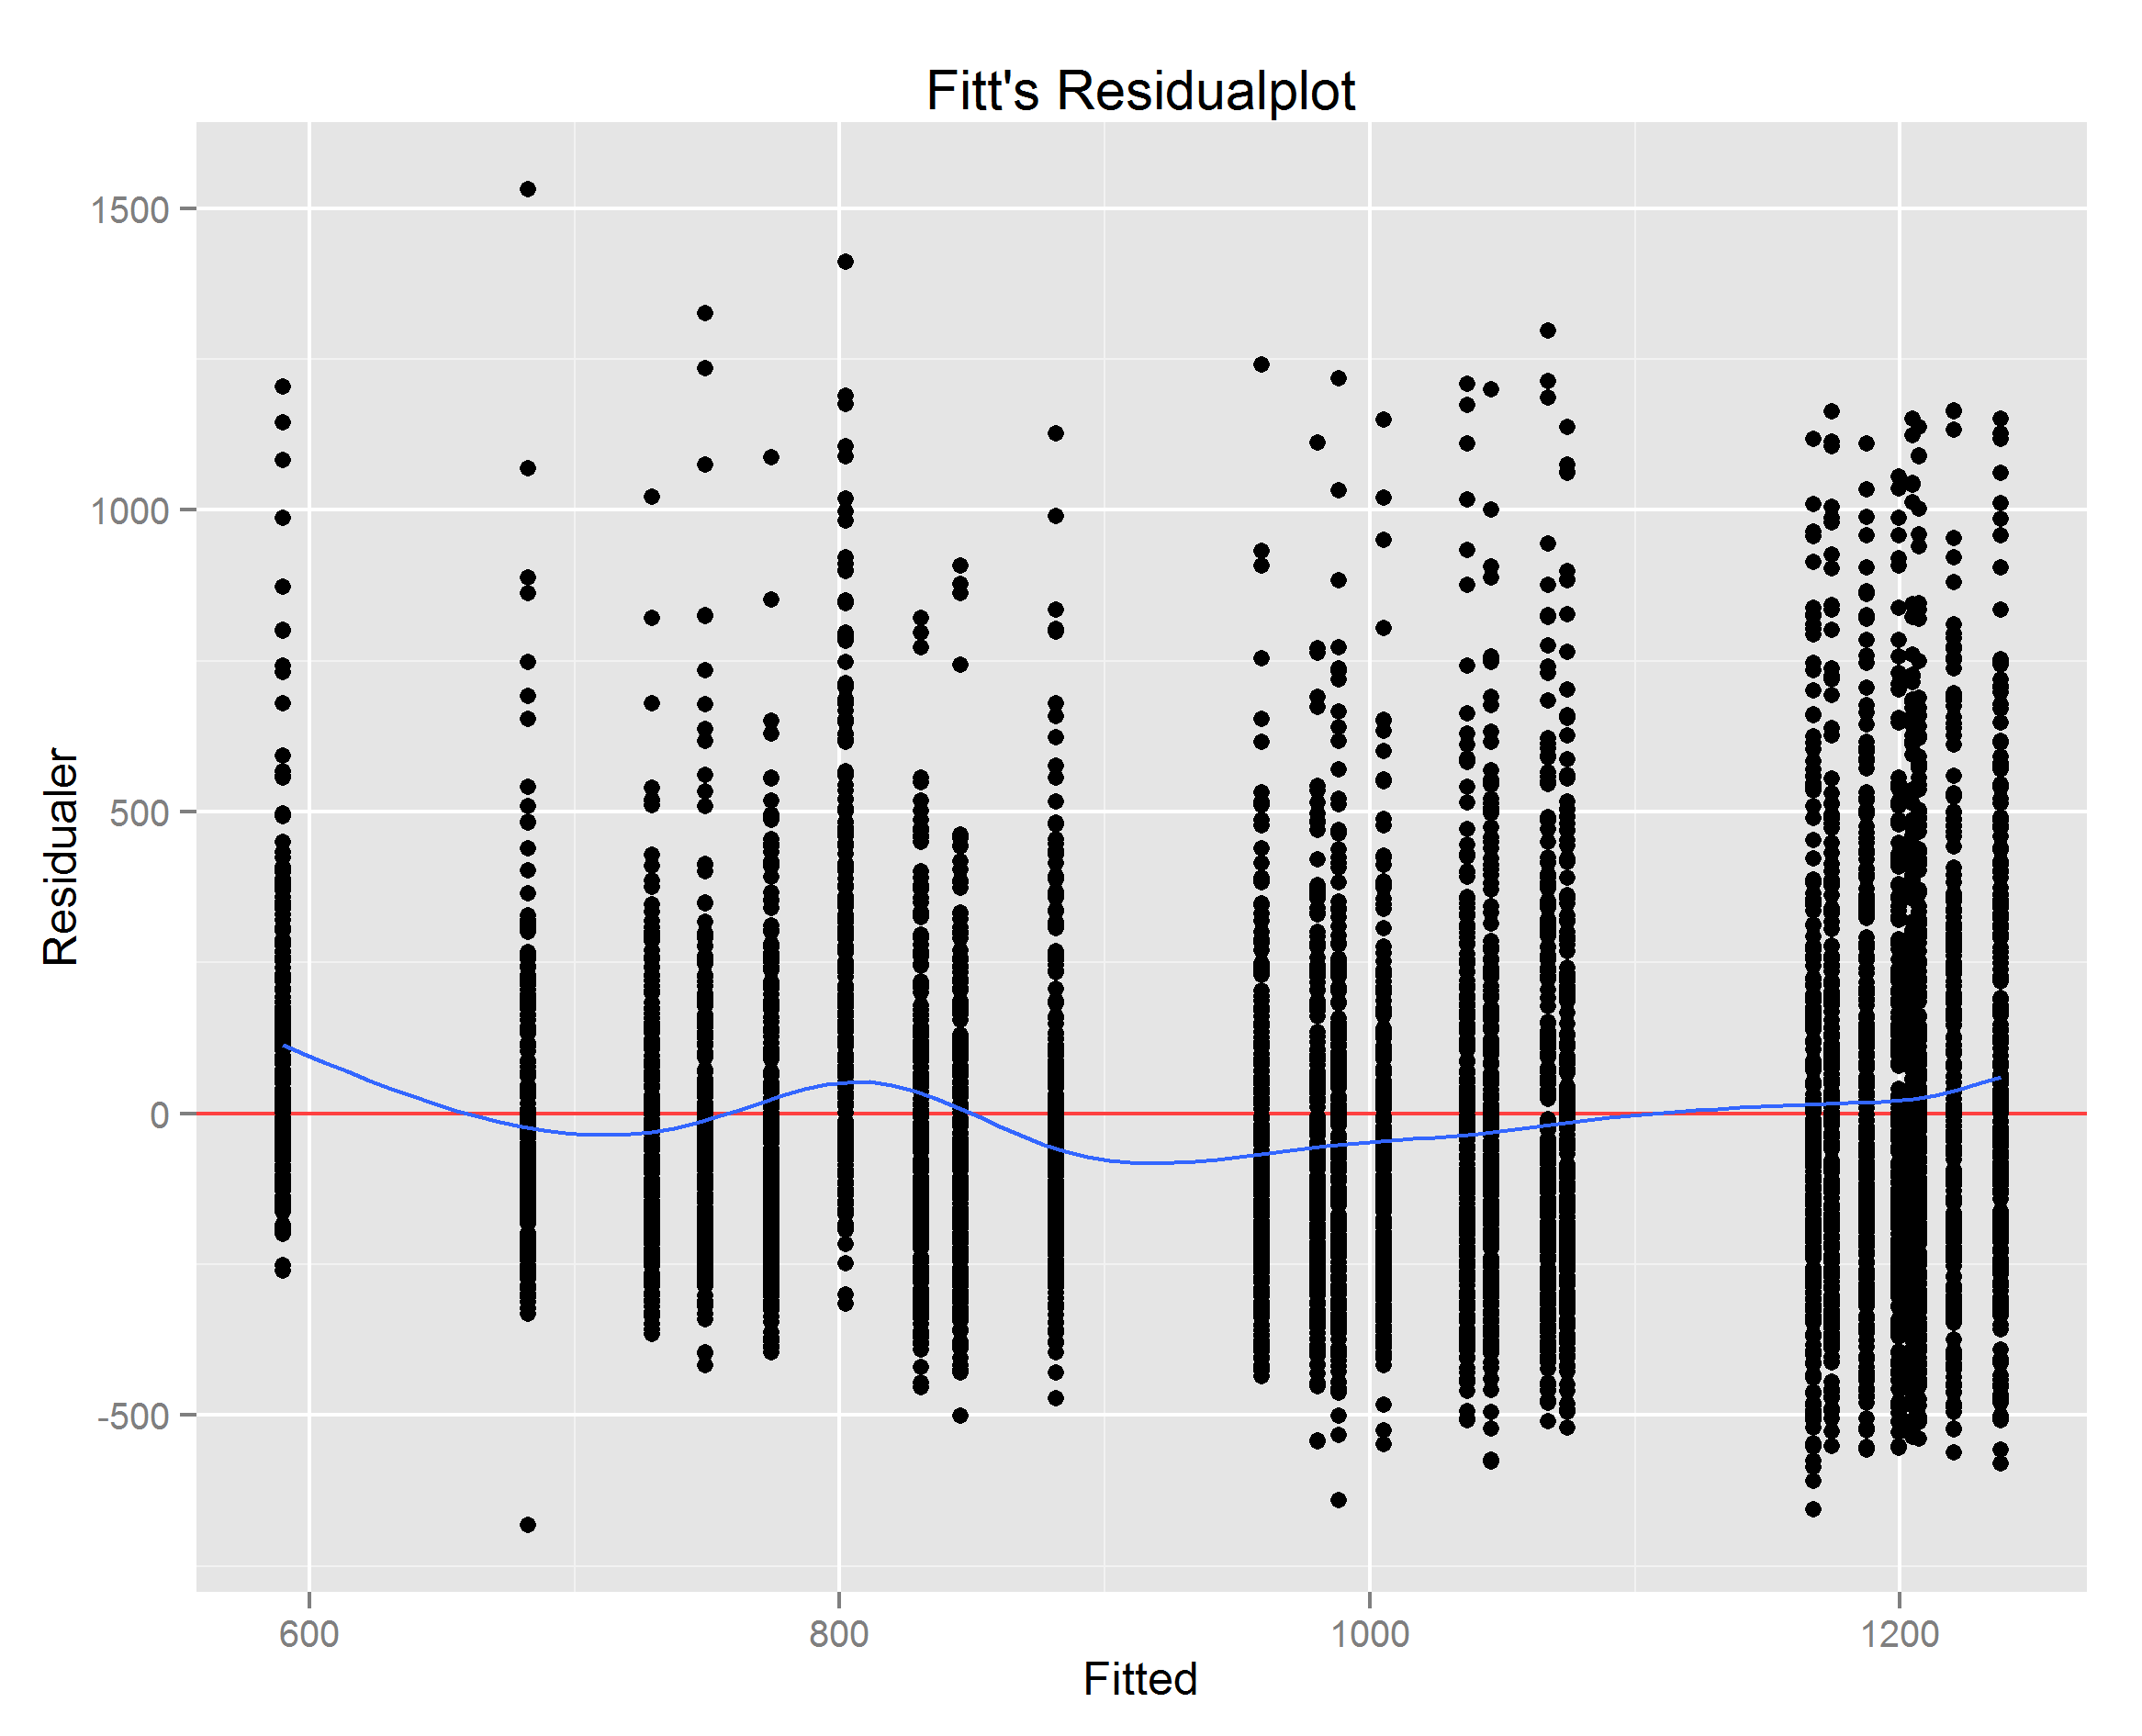
\includegraphics[width=\linewidth]{images/plots/plot_residual_fitt}
		\captionof{figure}{Fitts' residualplot}
		\label{fig:plot_residual_fitt}
	\end{minipage}
	\begin{minipage}{.5\linewidth}
		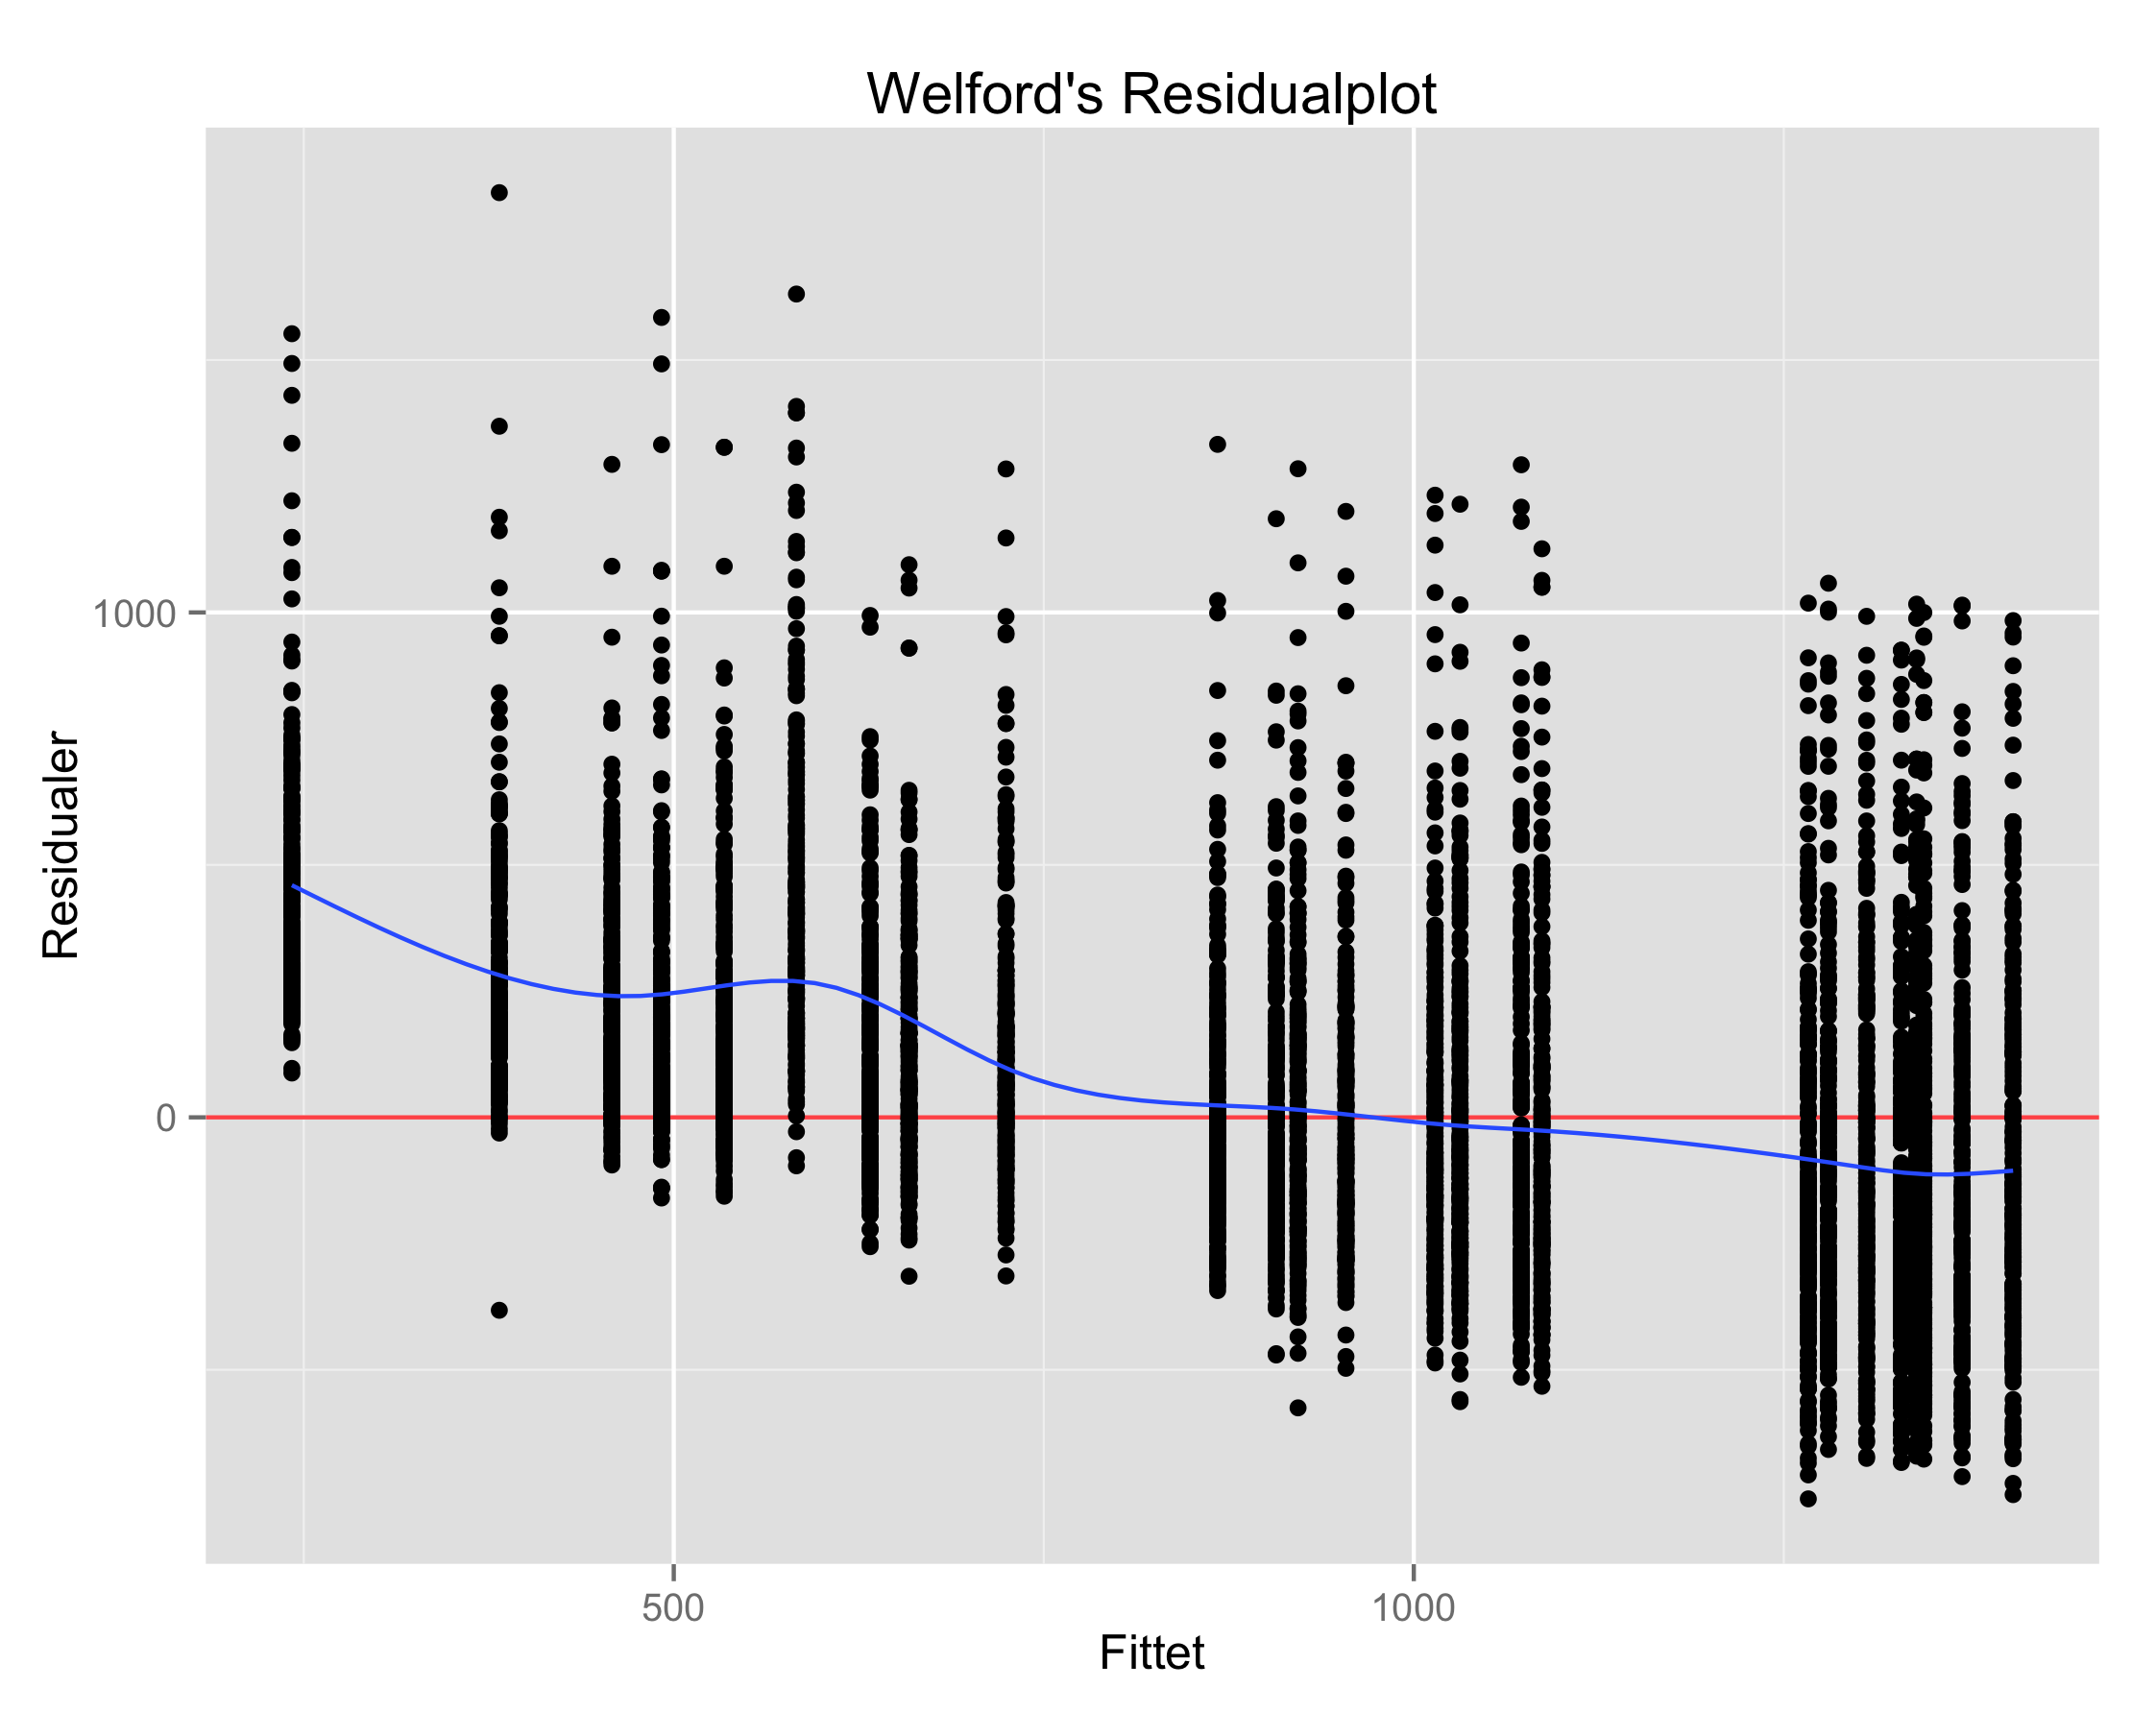
\includegraphics[width=\linewidth]{images/plots/plot_residual_welford}
		\captionof{figure}{Welford's residualplot}
		\label{fig:plot_residual_welford}
	\end{minipage}
	\begin{minipage}{.5\linewidth}
		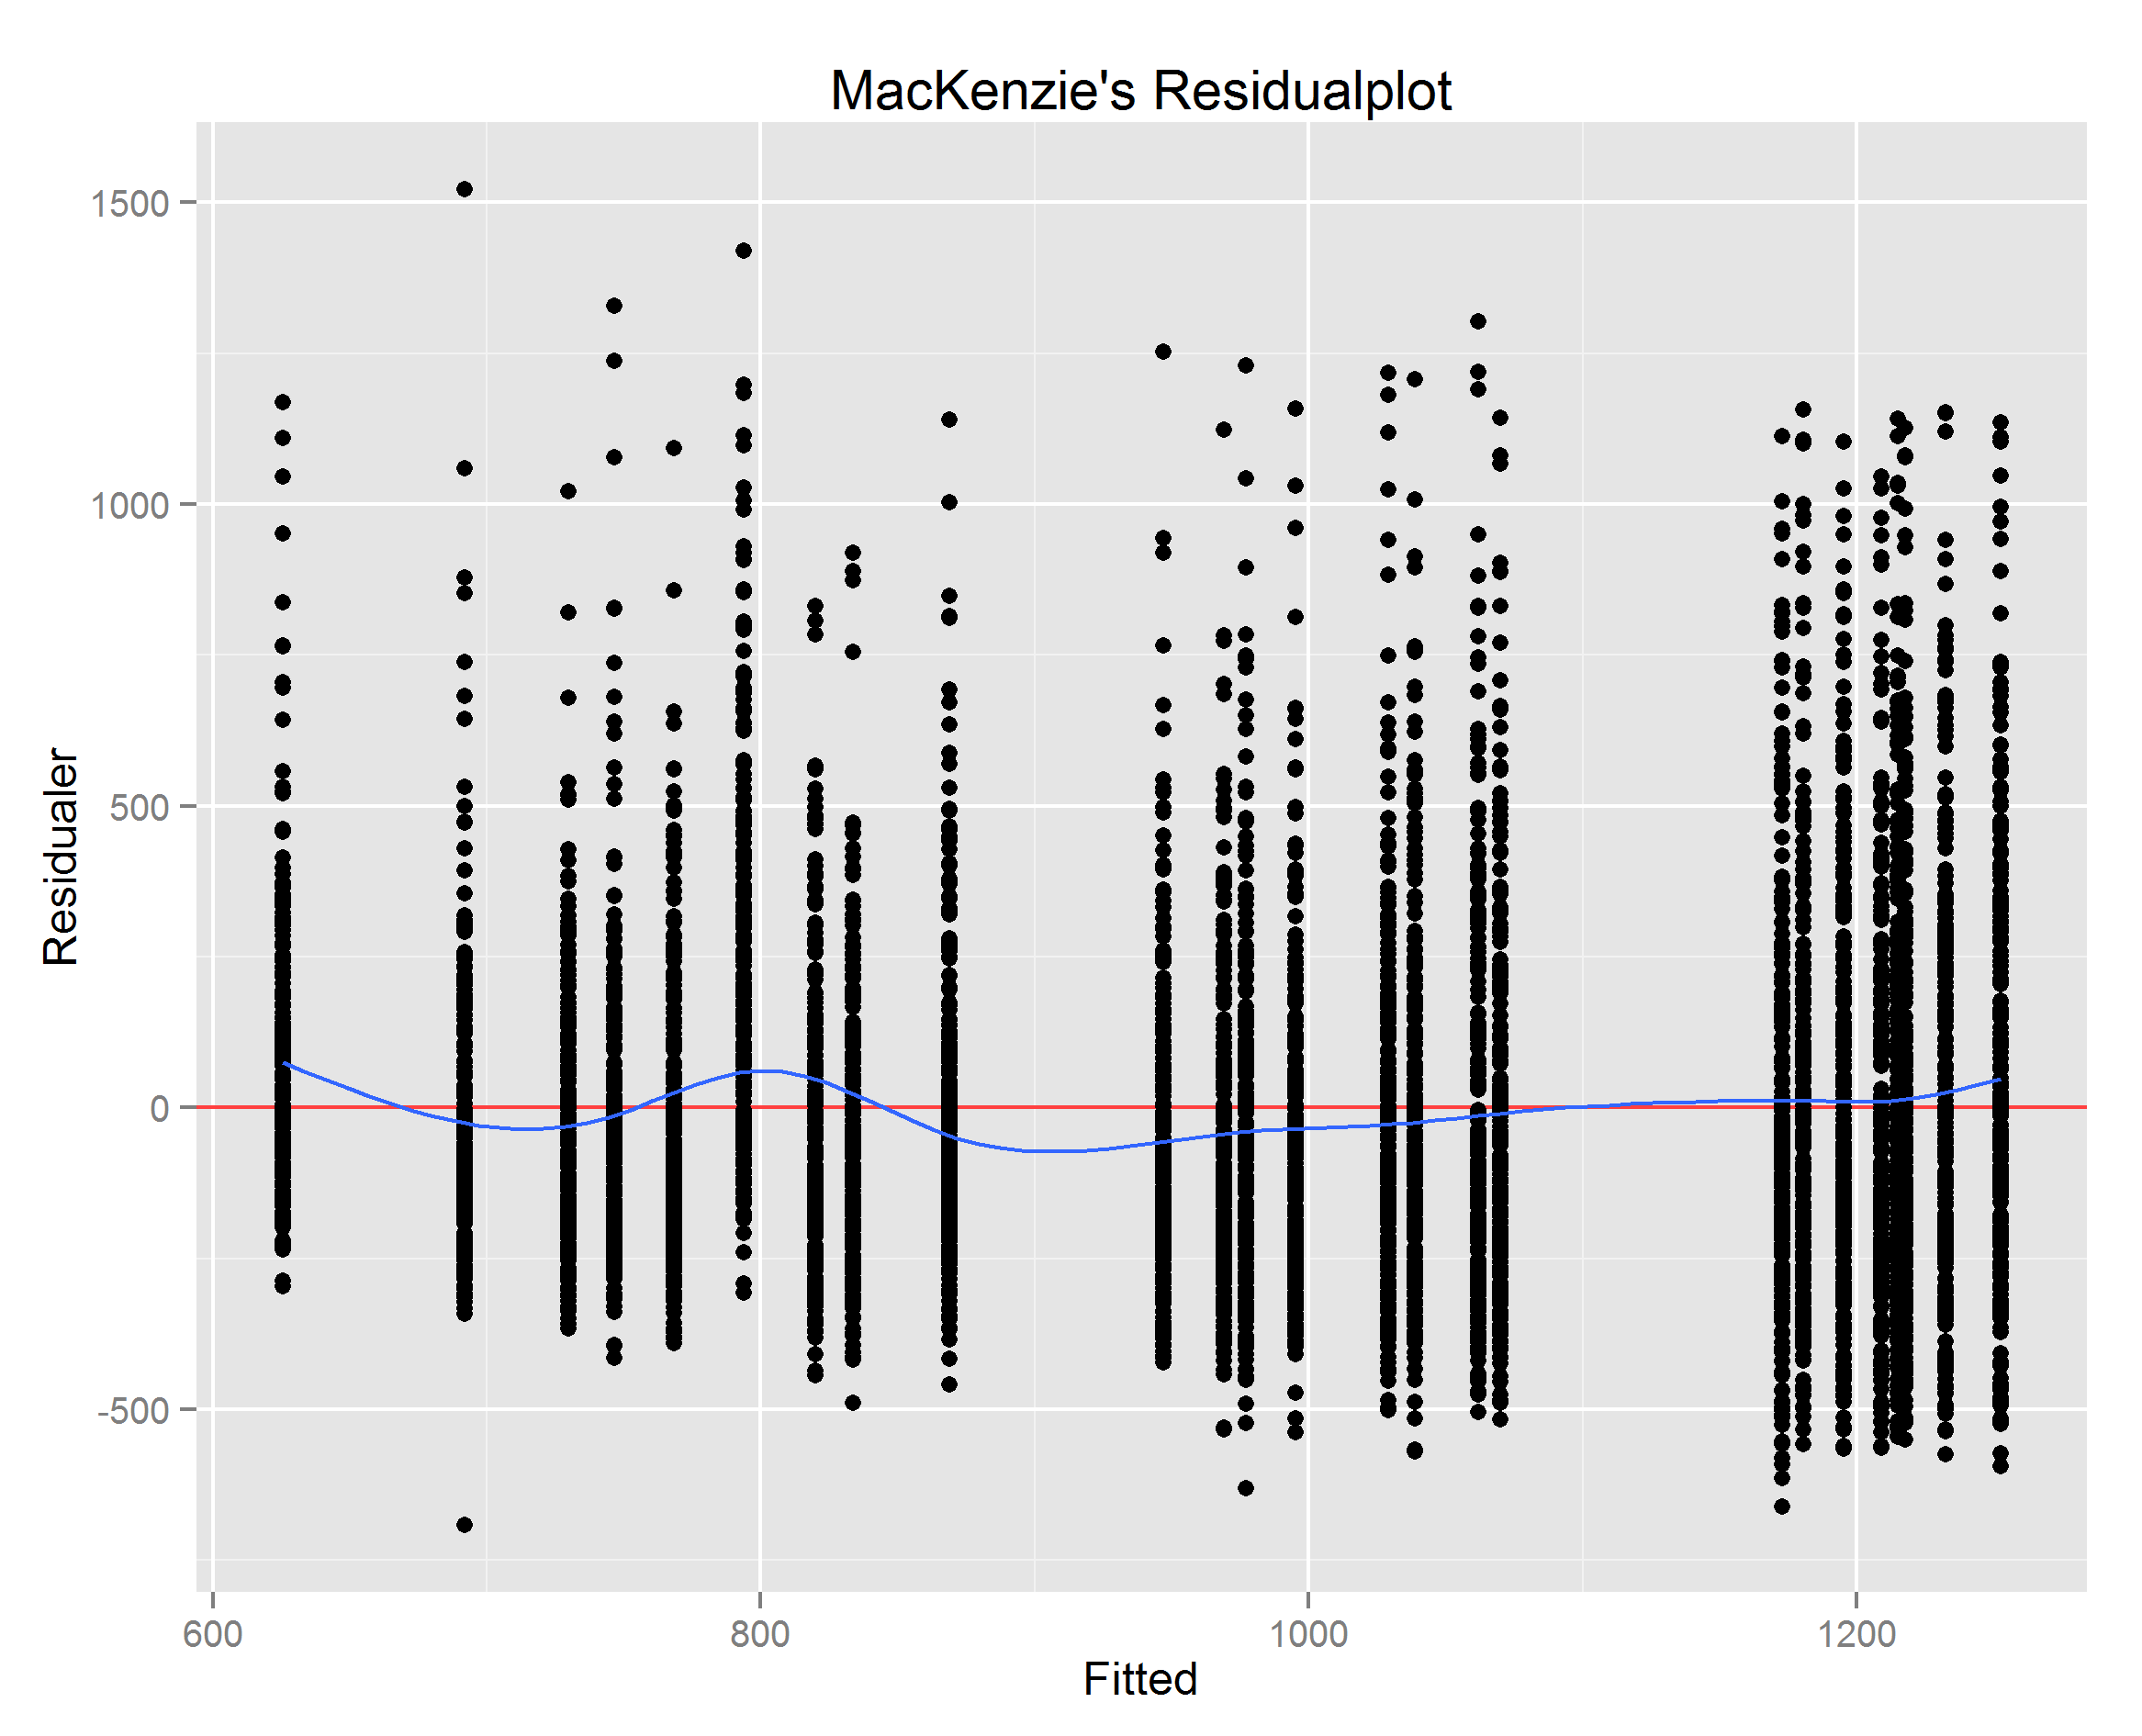
\includegraphics[width=\linewidth]{images/plots/plot_residual_mackenzie}
		\captionof{figure}{MacKenzie's residualplot}
		\label{fig:plot_residual_mackenzie}
	\end{minipage}
	\begin{minipage}{.5\linewidth}
		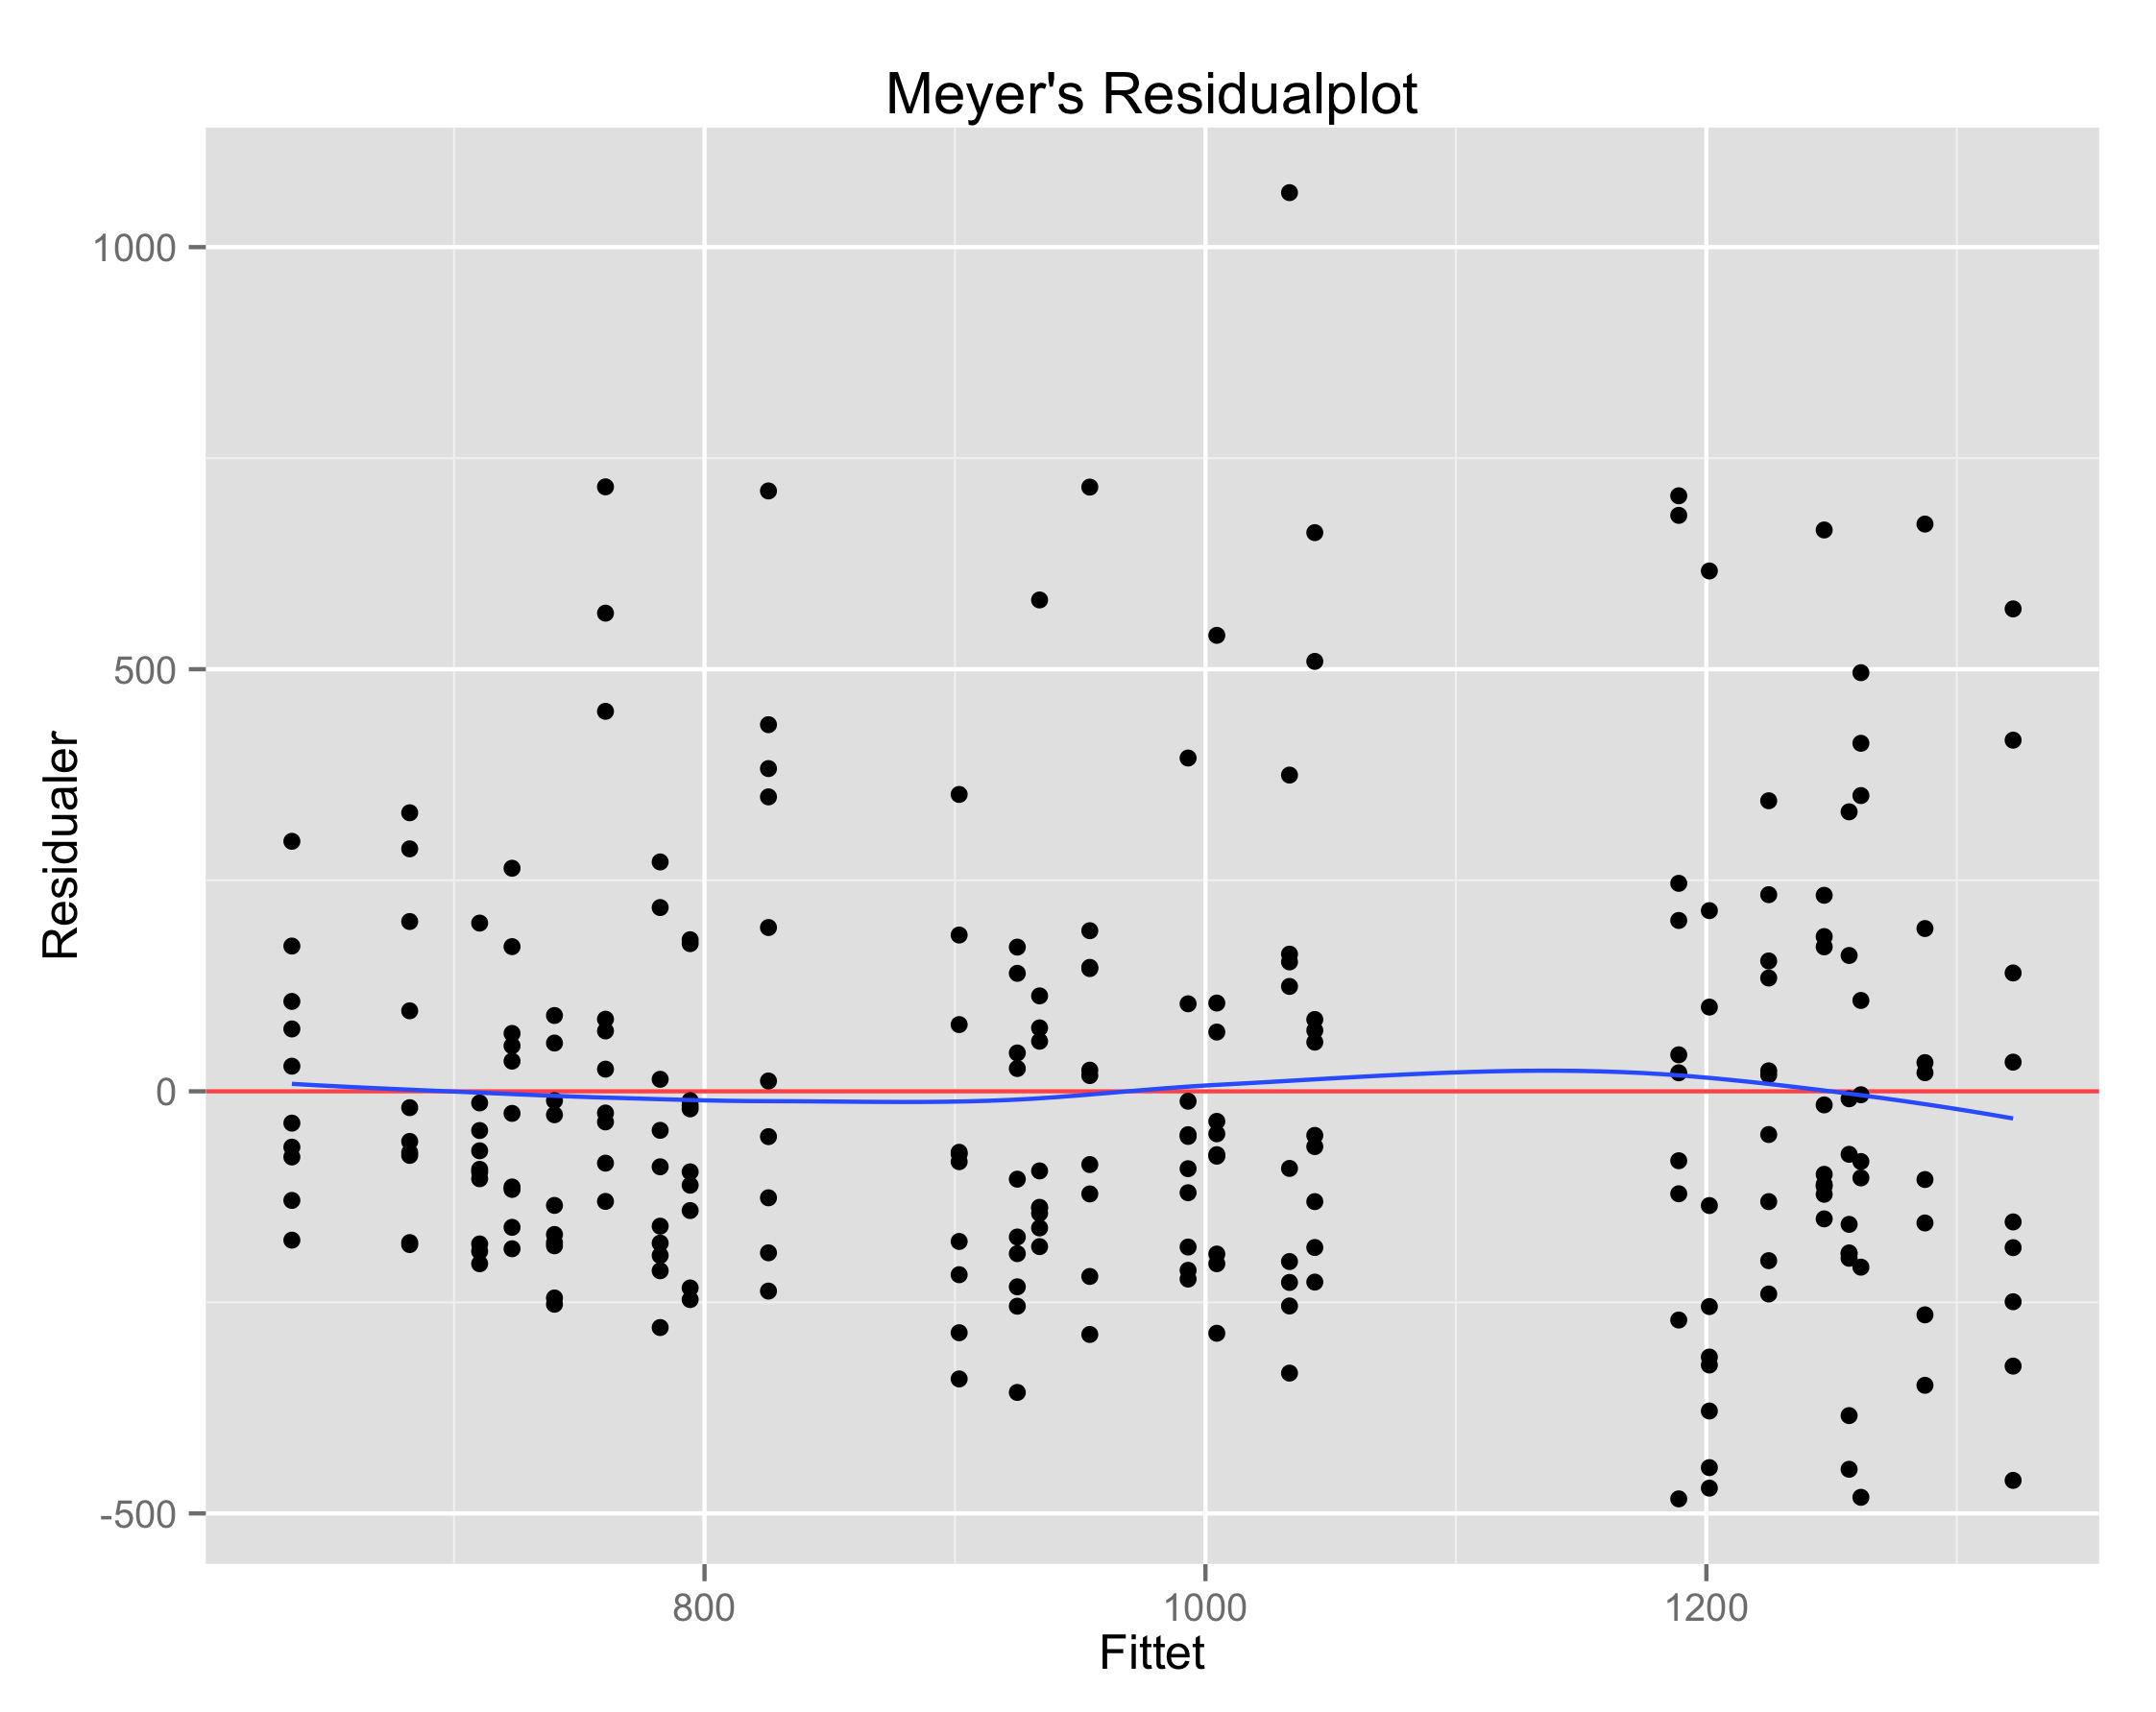
\includegraphics[width=\linewidth]{images/plots/plot_residual_meyer}
		\captionof{figure}{Meyer's residualplot}
		\label{fig:plot_residual_meyer}
	\end{minipage}
\end{minipage}

\addcontentsline{toc}{section}{Modelanalyse af navigationsopgaver}
\section*{Modelanalyse af navigationsopgaver}
I vores forsøg havde vi, udover pegeopgaven, også tunnel- og spiralopgaver. Vi vil i dette afsnit forsøge at tilpasse de fire formuleringer af Fitts lov på vores navigationsopgaver, velvidende om, at det ikke er den en type opgaver de er beregnet til. Accot og Zhai har i deres artikel \cite{accot1997} undersøgt lignende navigationsopgaver og fundet $ID$ specifikt for både tunnel- og spiralopgaver, hvilket vi vil bruge til at sammenligne med de fire formuleringer.

\addcontentsline{toc}{subsection}{Analyse af tunnelopgaver}
\subsection*{Analyse af tunnelopgaver}
De fire formuleringer er, som benævnt, ikke lavet til navigationsopgaver, vi har dog alligevel tilpasset en lineær model med deres respektive ID, til vores tunneldata. Vi har valgt afstanden, $A$, til at være længden på tunnellen, og bredden, $W$, til at være størrelse på tunnelens højre lodrette linje, slutstregen, som altid er $8$ pixels. Ved lineær regression, $lm()$, med $R$ fik vi tilpasset nedenstående matematiske modeller af de fire formuleringer.

\begin{align*}
\text{Fitts': } &T = 3532.2 + 581.9\cdot \log_2\left(\frac{2A}{W}\right)\\
\text{Welford's: } &T =  1242.58\cdot \log_2\left(\frac{A+\frac{1}{2}W}{W}\right)\\
\text{Mackenzie's: } &T = 4036.7 + 592.3\cdot \log_2\left(\frac{A+W}{W}\right)\\
\text{Meyer's: } &T = 5863.07 + 210.48 \cdot \sqrt{\frac{A}{W}}
\end{align*}

Helt naturligt er det additive led markant højere for tunnelopgaverne end for pegeopgaverne, da det gennemsnitligt har taget længere tid for vores testdeltagere at gennemføre dem. Gennemsnittet for tunnelopgaverne er på $7673.01$ millisekunder og $983.30$ millisekunder for pegeopgaverne. Det additive led kan dog ikke fortolkes som reaktionstiden for tunnelopgaverne, da tiden starter når testdeltageren passere venstre lodrette streg og derfor allerede er i bevægelse.

Accot og Zhai beskriver i deres artikel \cite{accot1997}, hvordan en indsnævrende tunnelopgave kan opdeles i små delelementer, som hver især udgør én lille navigationsopgave. Ved at gøre dette kan man finde $ID$ som summen af delelementernes $ID$, hvilket resulterer i $ID_{NT} = \frac{A}{W_2-W_1}\ln\left(\frac{W_2}{W_1}\right)$, hvor $W_1$ er størrelsen på venstre lodrette streg, startstregen, og $W_2$ er størrelsen på højre lodrette streg, slutstregen. I følge Accot og Zhai er der en lineær afhængighed imellem tiden $T$ og dette $ID_{NT}$, hvilket giver anledning til følgende matematiske formulering $T = a+b\cdot ID_{NT}$. Tilpasses denne formulering med lineær regression til vores filtrerede datasæt får vi nedenstående model.

\begin{align*}
\text{Accot \& Zhai: } T = 6112.40+47.77 \cdot \left(\frac{A}{W_2-W_1}\cdot\ln\left(\frac{W_2}{W_1 }\right)\right)
\end{align*}

Det kan bemærkes, at den primære forskel imellem Accot og Zhai's formulering og de fire andre er det multiplikative led, $b$. Da $ID_{NT}$ antager væsentligt højere værdier er $b$ tilsvarende mindre. De fem affine modeller har vi valgt at plotte i forhold til gennemsnittet af tiden for hvert $ID$, for bedre at visualisere, modellernes præcision. Plottene kan ses i figur \ref{fig:welford_tunnel_line}, \ref{fig:fitt_tunnel_line}, \ref{fig:meyer_tunnel_line},\ref{fig:mackenzie_tunnel_line} og \ref{fig:accot_tunnel_line}. På $x$-aksen er modellens respektive $ID$ imens tiden, $T$, for at løse en opgave er givet ved $y$-aksen.

Af graferne ser det ud til, at Welfords klarer sig markant dårligere end de fire andre formuleringer, som til gengæld ikke har nogen umiddelbar forskel. AIC analysen, \ref{tab:table_analysis_aic_tunnel} af de fem modeller viser netop dette, hvor Meyer's model klarer sig bedst, men med utrolig lille indbyrdes forskel imellem de bedste fire modeller. Kun Welford's formulering har en relativt markant dårligere præcision til dataene.

\begin{table}[h]
\centering
\begin{tabular}{lll}
Model & AIC værdi & Forskel\\\hline
Meyer & 20549.61 & 0 \\
Accot \& Zhai & 20549.62 & 0.01\\
Fitts & 20549.68 & 0.07\\
Mackenzie & 20549.68 & 0.07 \\
Welford & 20558.46 & 8.84
\end{tabular}
\caption{AIC værdier og indbyrdes forskel med udgangspunkt i Fitts' som nulpunkt}
\label{tab:table_analysis_aic_tunnel}
\end{table}

Hvis vi forsøger at tilpasse Accot og Zhai's formulering til vores kontrollerede testpersoners individuelle data, så kan det vises, hvor afvigende vores data for disse opgaver er. Figur \ref{fig:navigationtest1} viser den traditionelle stigning i tiden med tilsvarende stigning i $ID$, men på figur \ref{fig:navigationtest2} kan det ses, hvordan datapunkterne opfører sig stik modsat. Det vil sige, at testperson 9 var hurtigere til at klare opgaverne i takt med, at de blev sværere.

\begin{minipage}{\linewidth}
	\begin{minipage}[b]{.45\linewidth}
		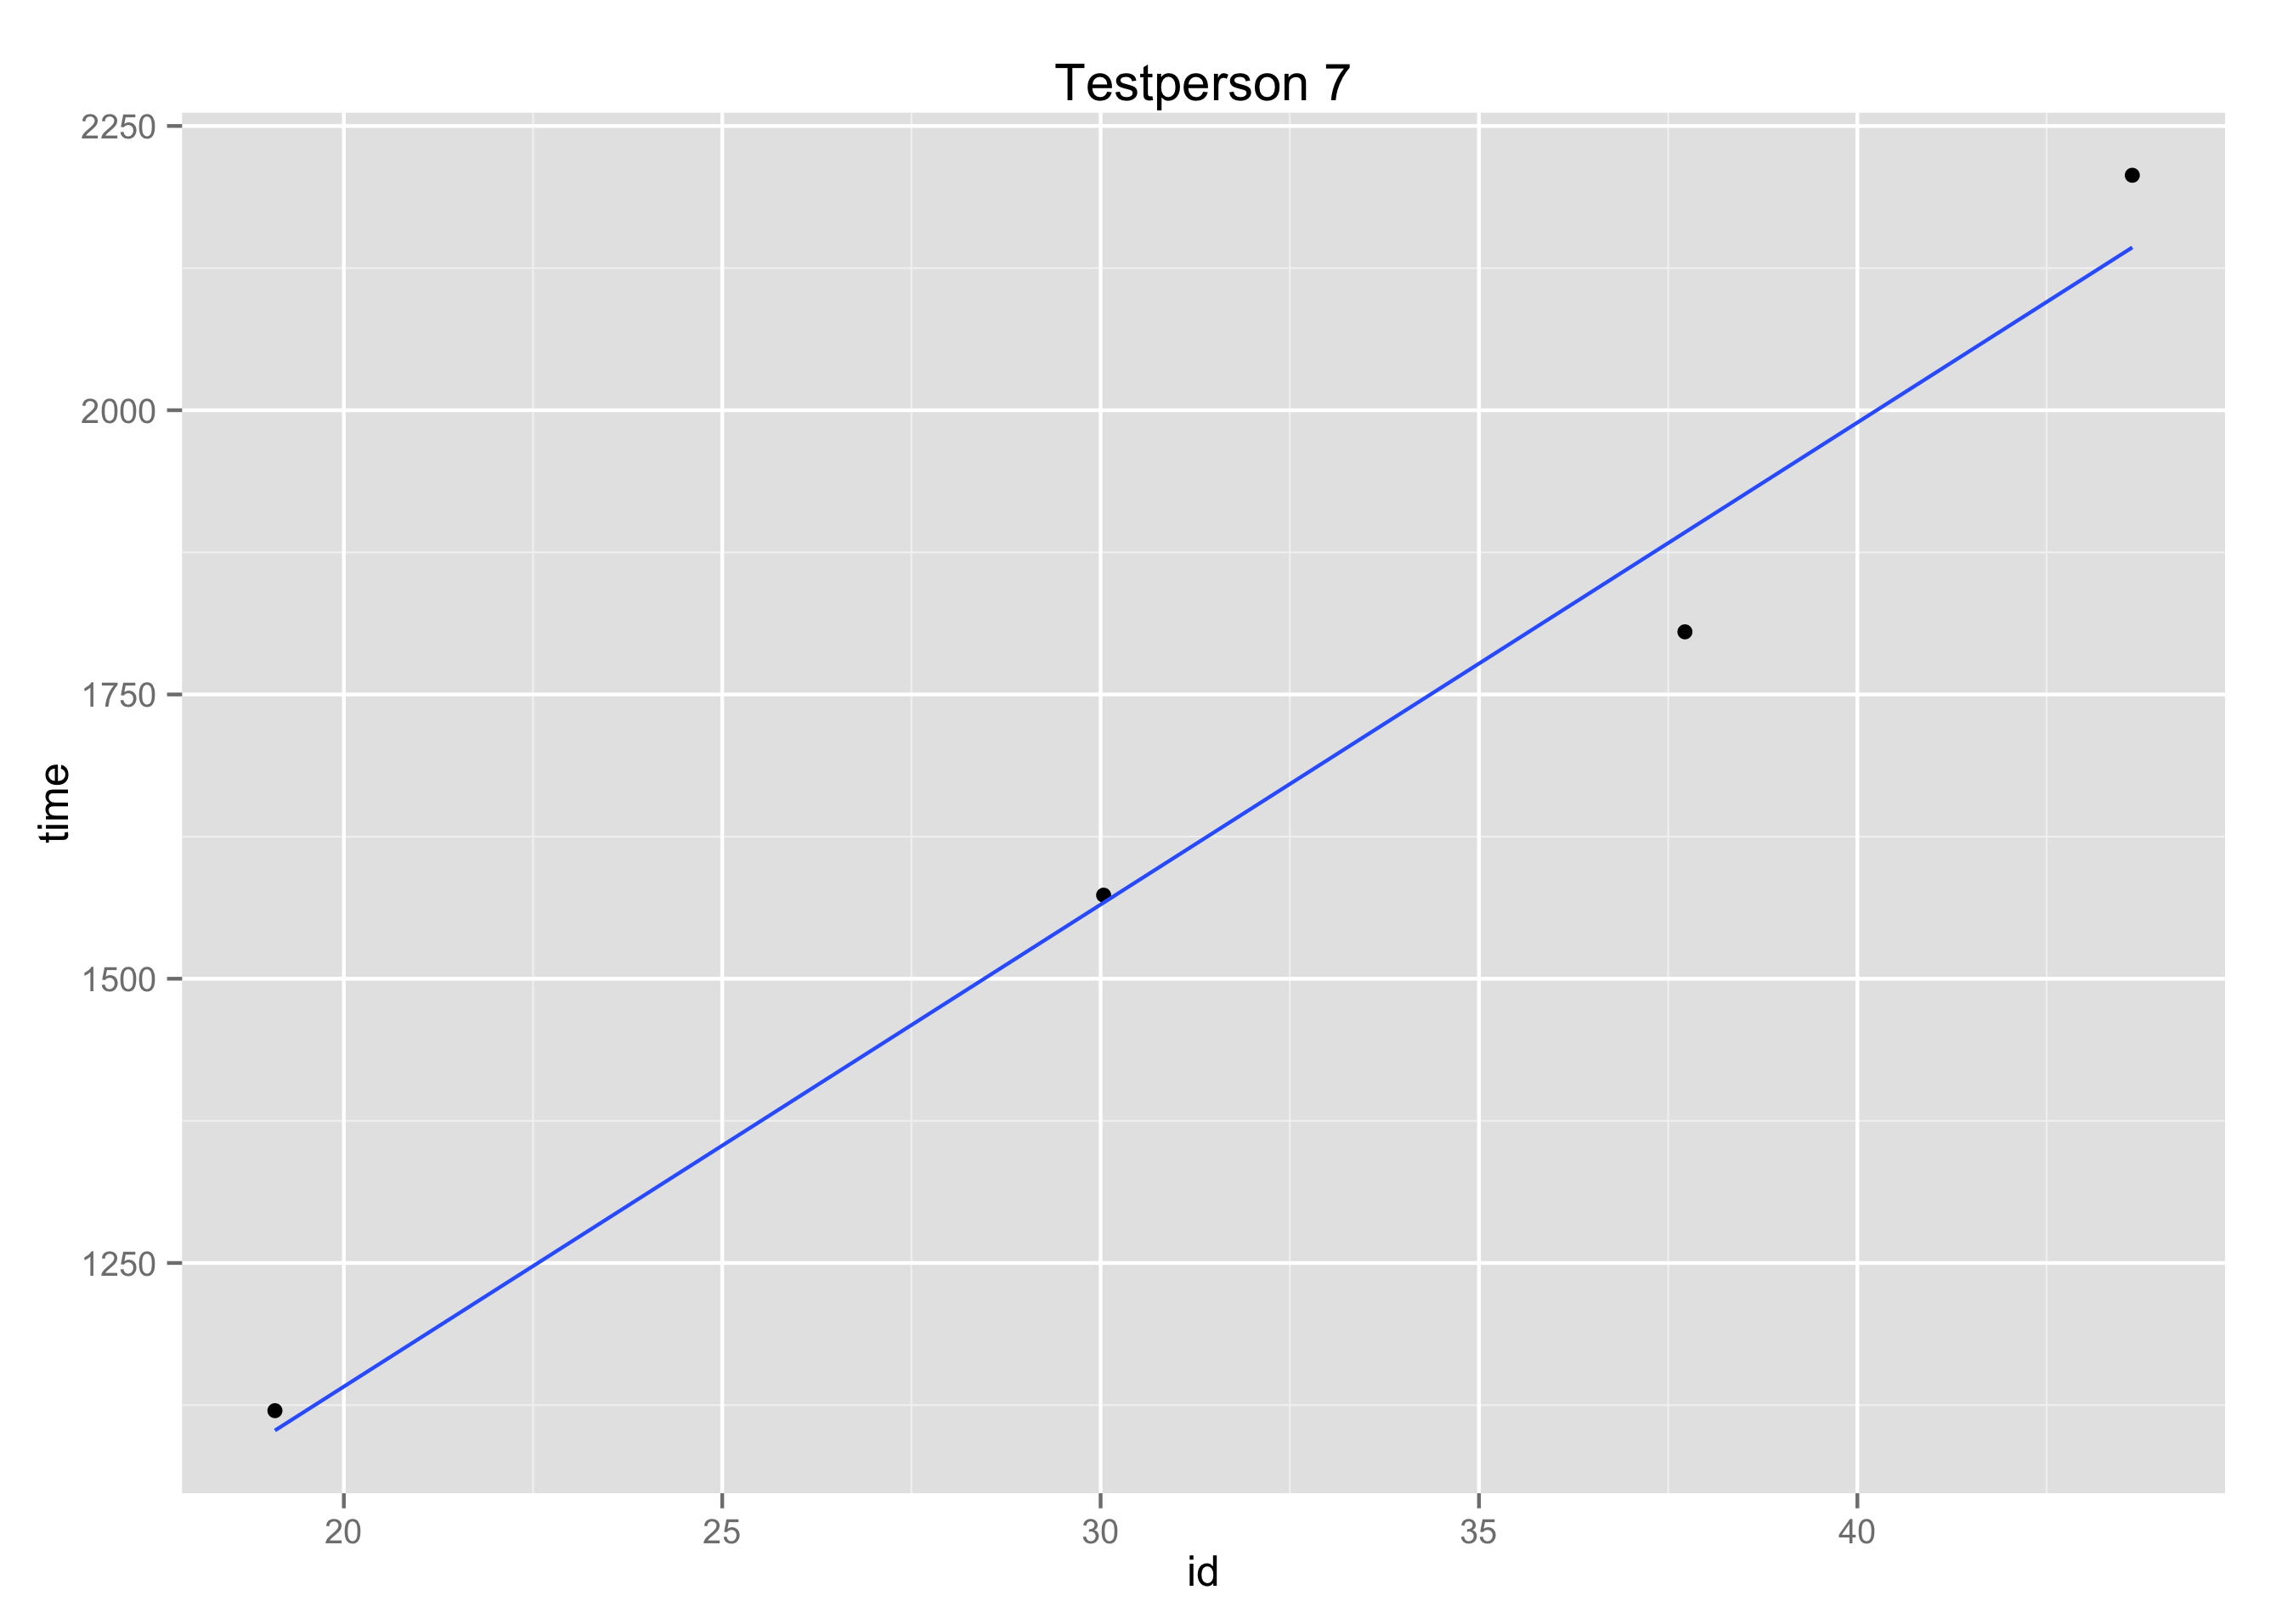
\includegraphics[width=\textwidth]{images/plots/plot_model_test_navigation_1}
		\captionof{figure}{Accot og Zhai's formulering tilpasset til testperson 7, med $ID$ på $x$-aksen og tiden $T$ på $y$-aksen.}
		\label{fig:navigationtest1}
	\end{minipage}
	\begin{minipage}[b]{0.1\linewidth}
	~
	\end{minipage}
	\begin{minipage}[b]{0.45\linewidth}
		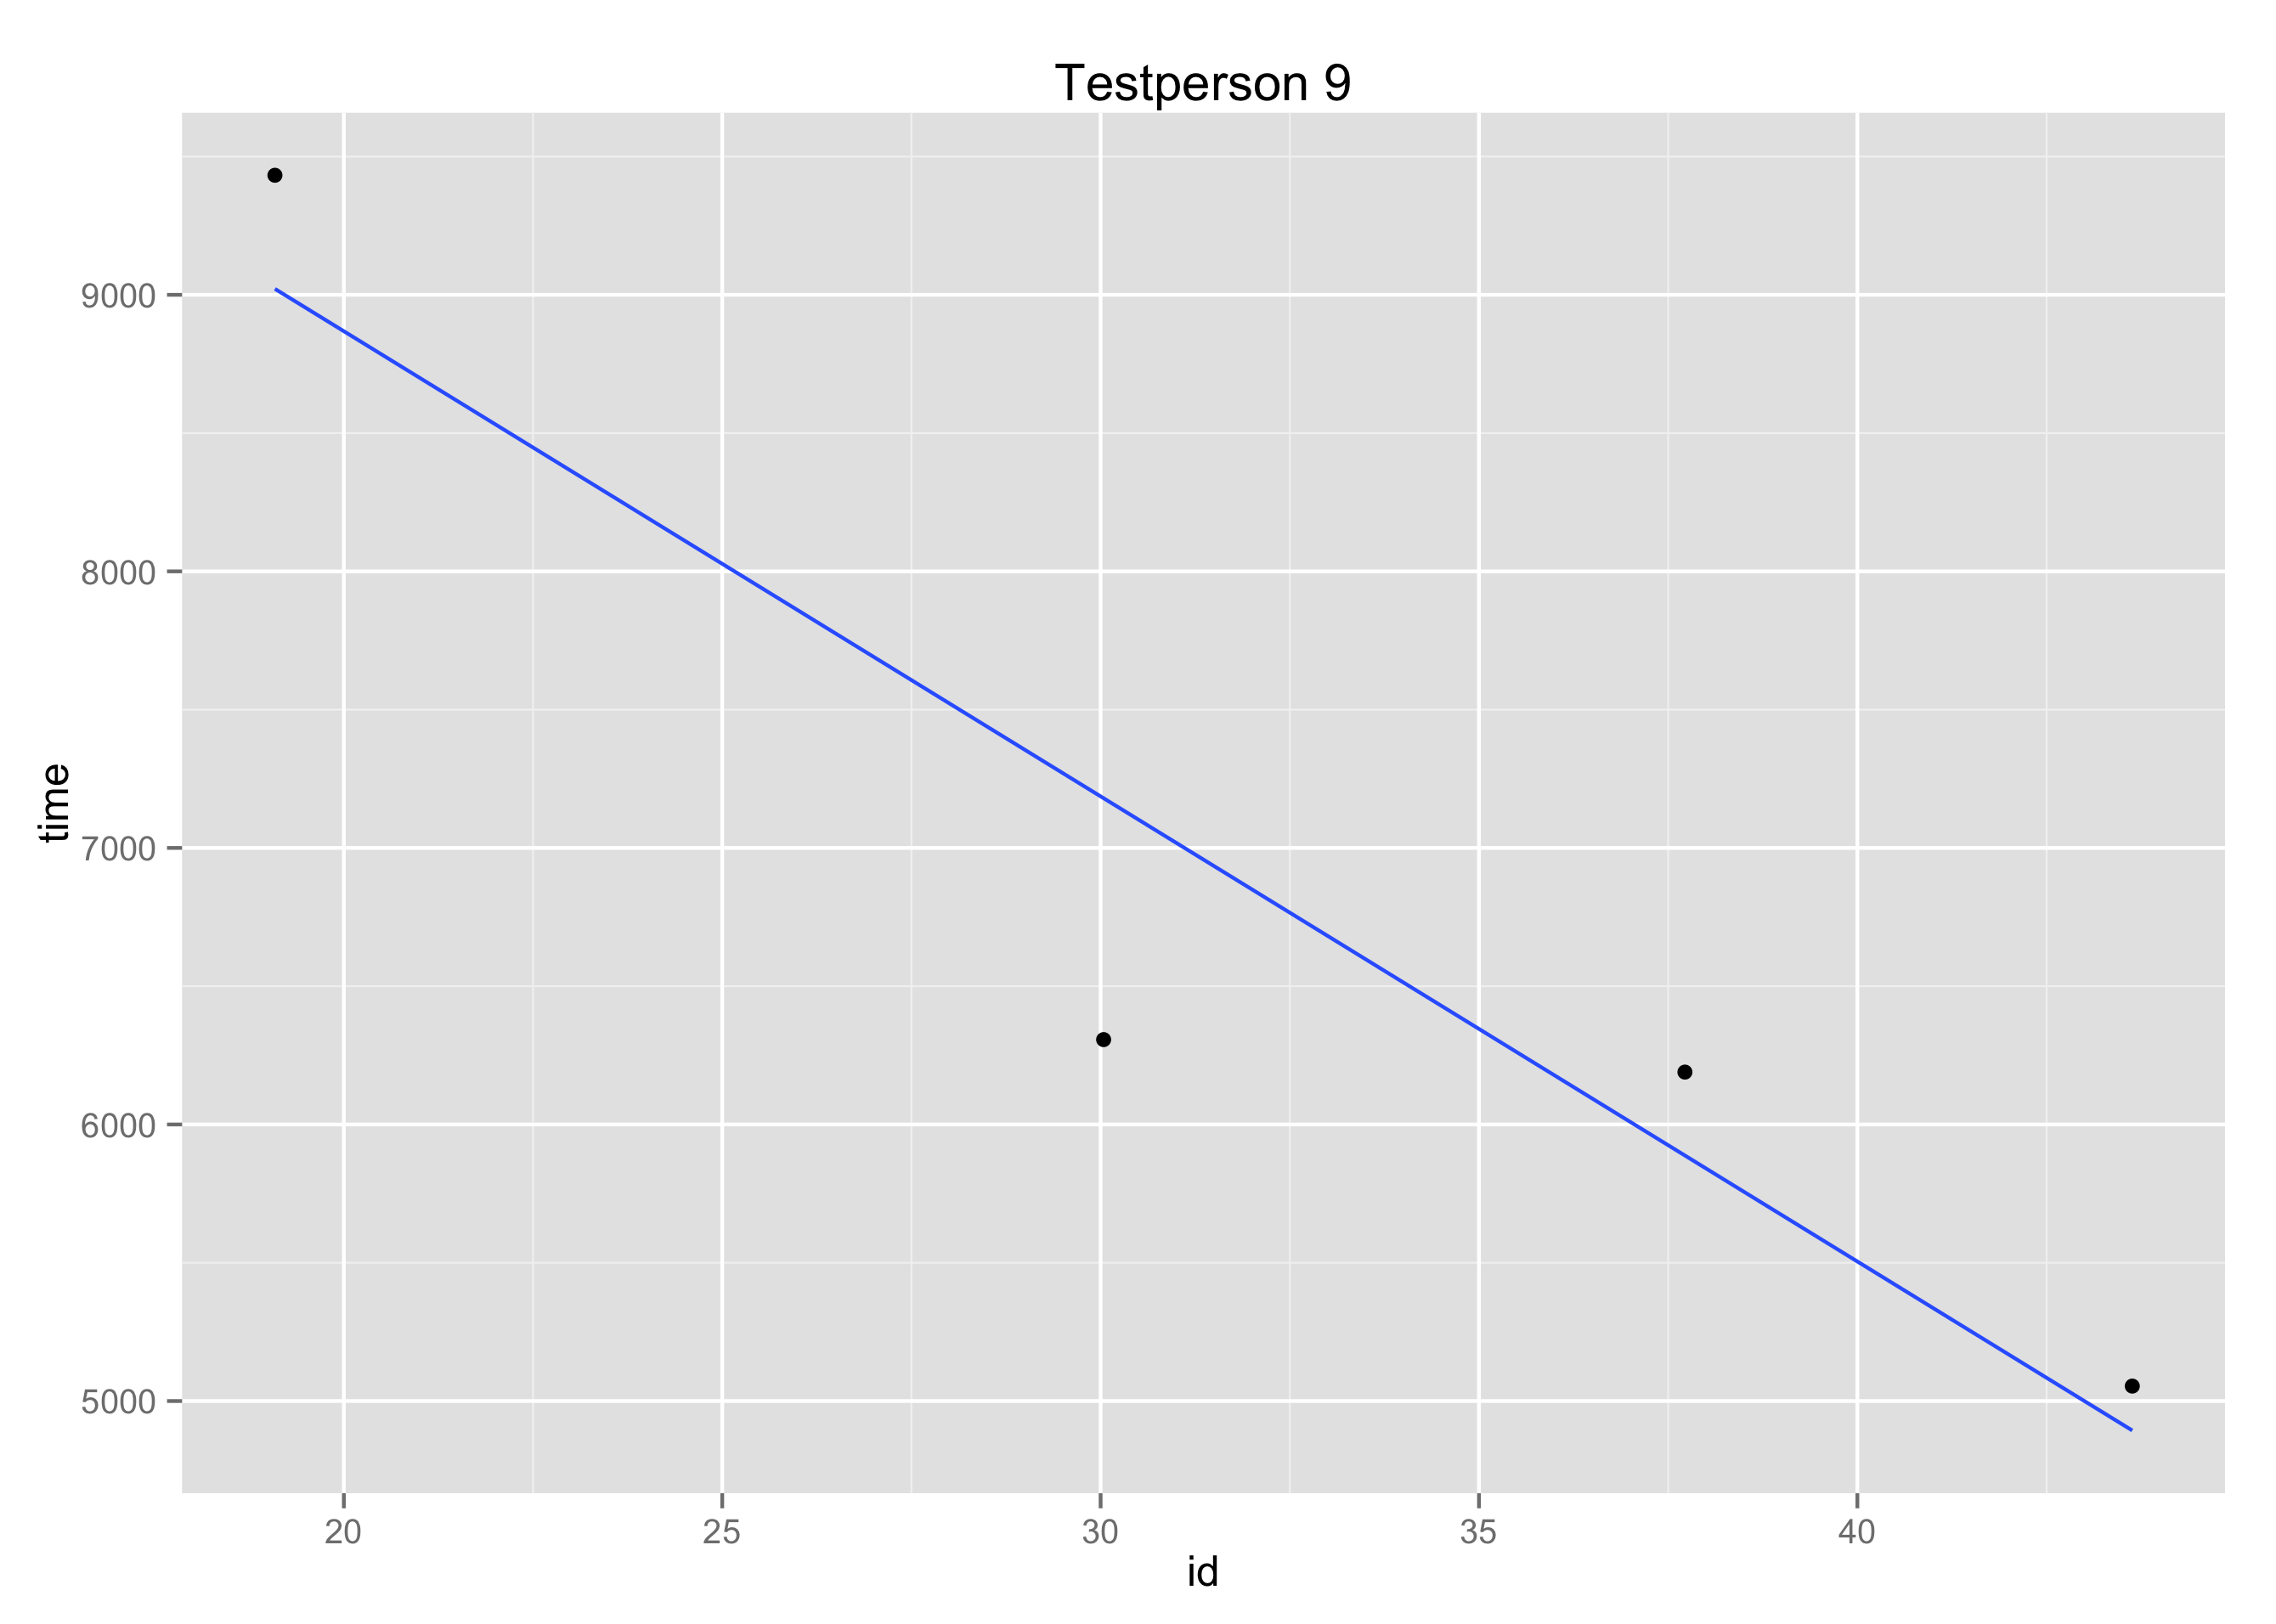
\includegraphics[width=\textwidth]{images/plots/plot_model_test_navigation_2}
		\captionof{figure}{Accot og Zhai's formulering tilpasset til testperson 9, med $ID$ på $x$-aksen og tiden $T$ på $y$-aksen.}
		\label{fig:navigationtest2}
	\end{minipage}
\end{minipage}

\begin{minipage}{\linewidth}
	\begin{minipage}[t]{.45\linewidth}
		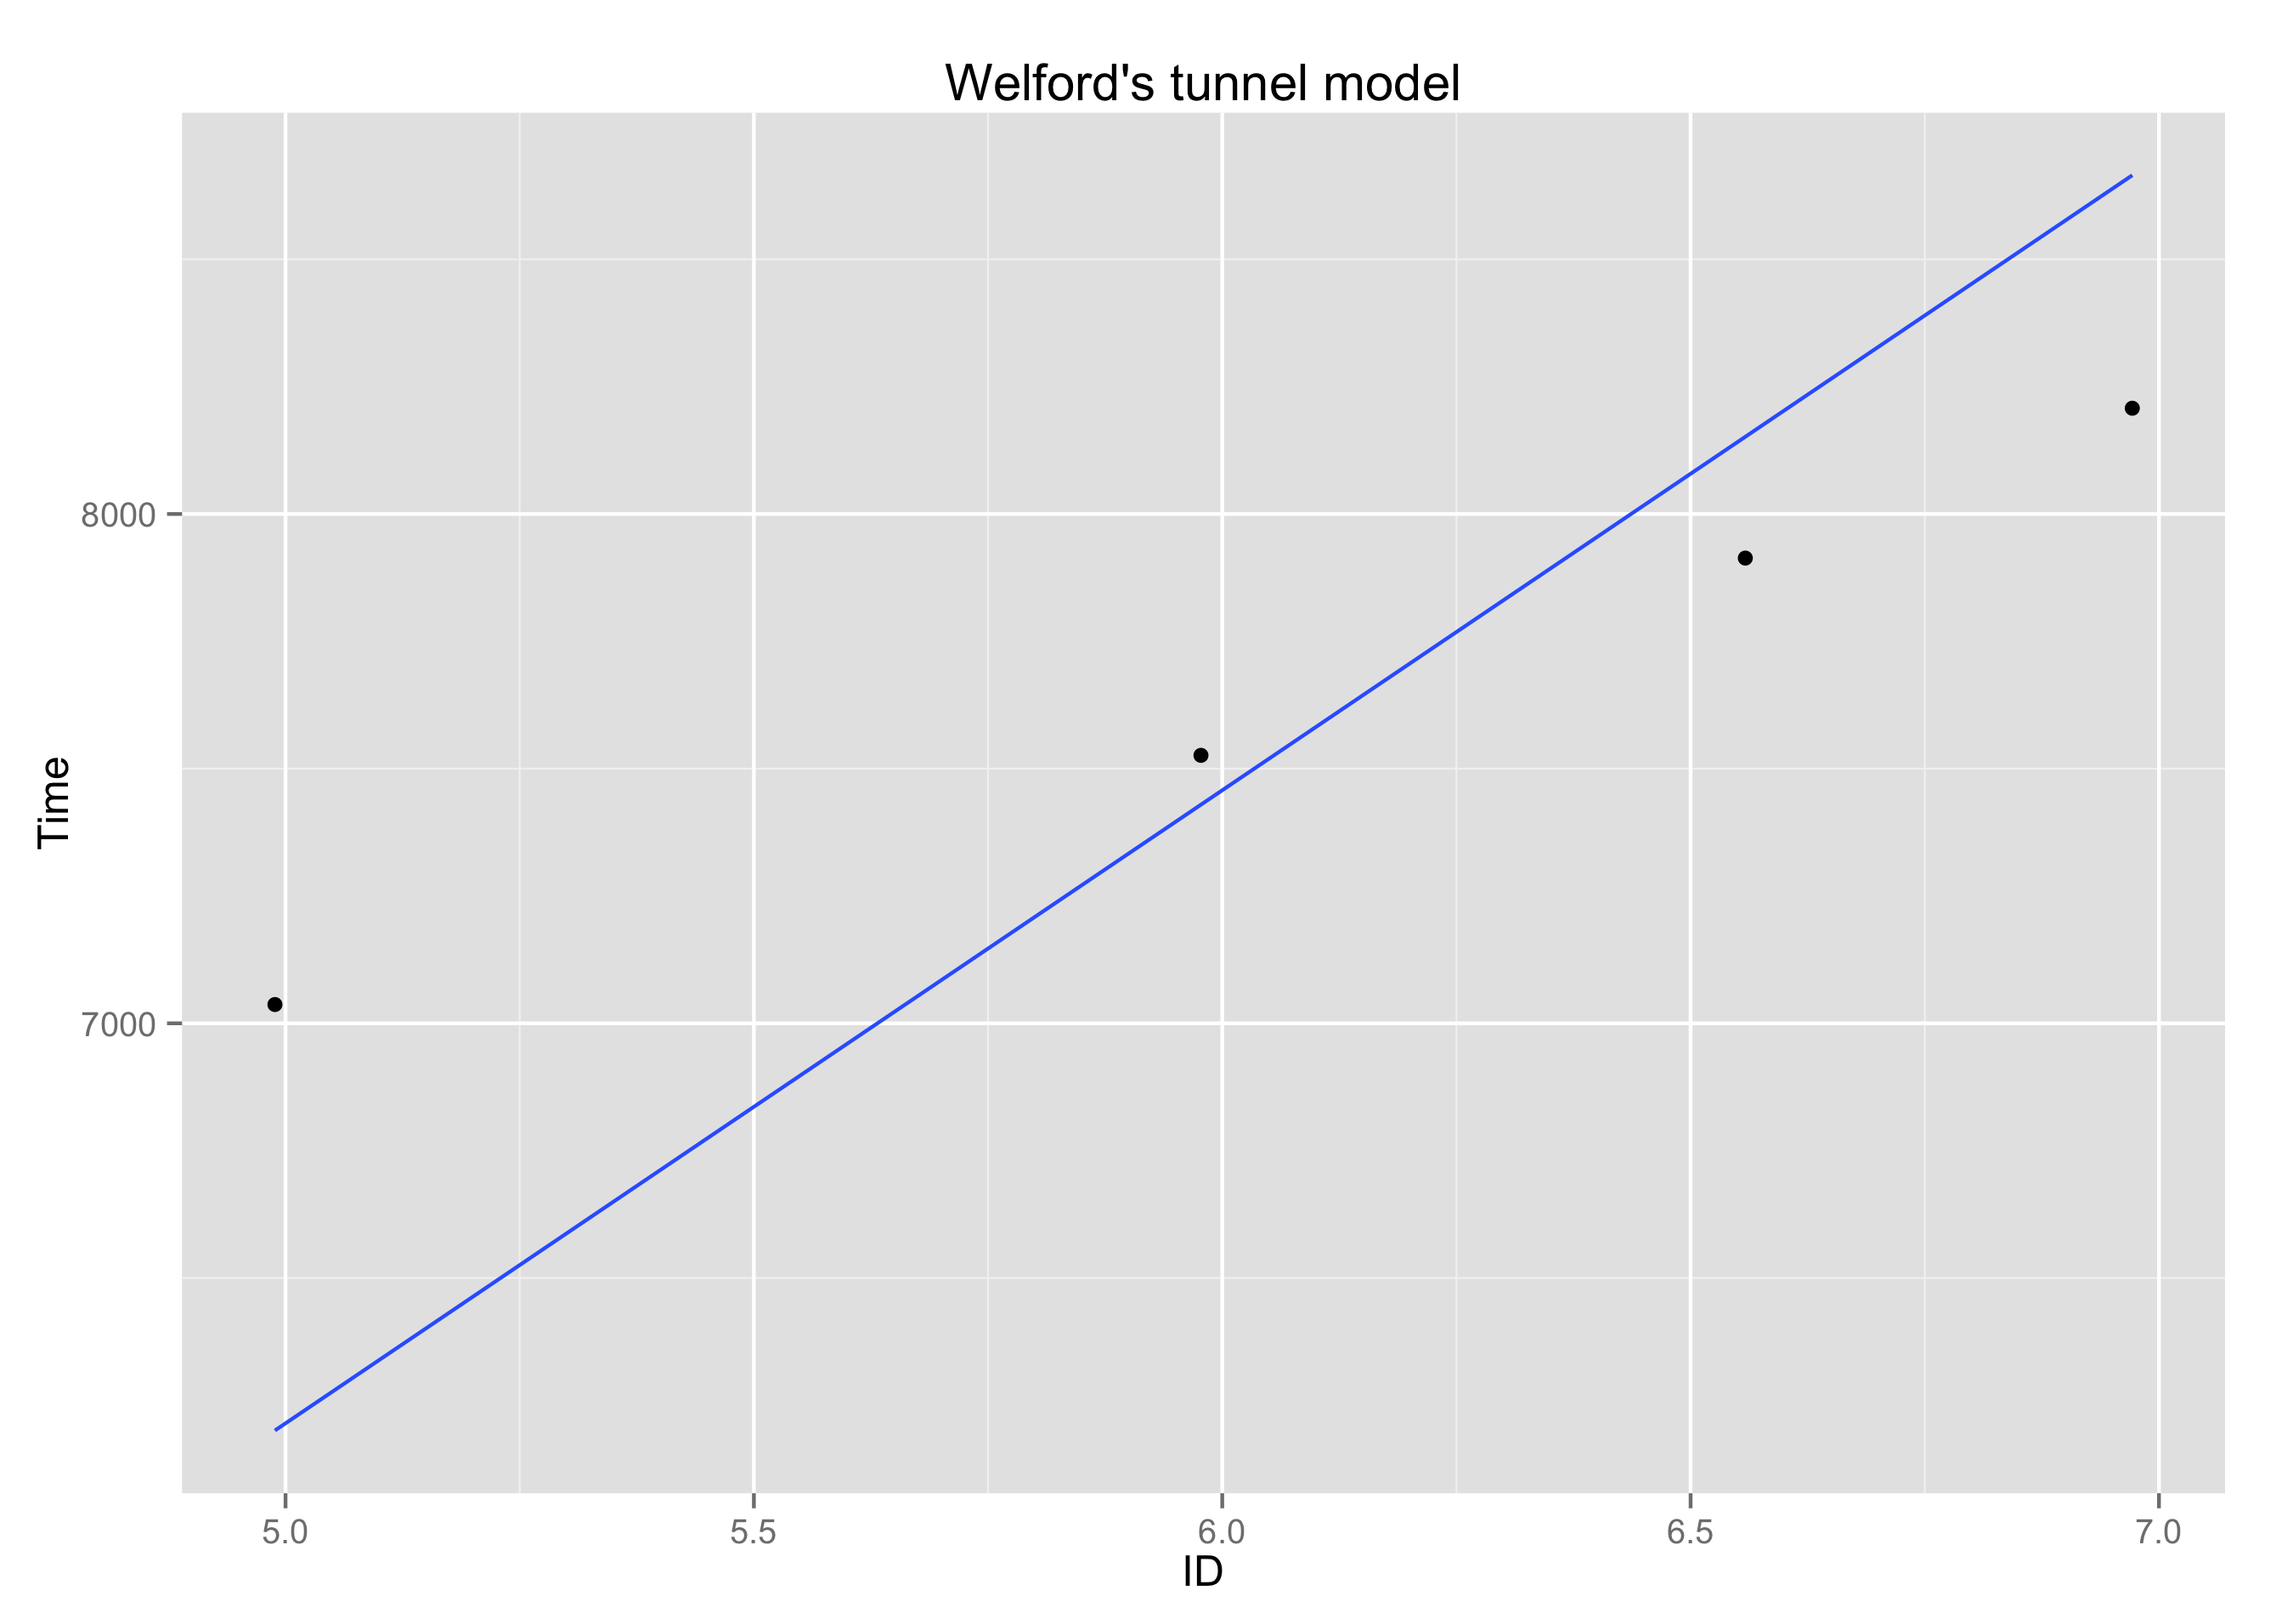
\includegraphics[width=\textwidth]{images/plots/plot_model_tunnel_welford}
		\captionof{figure}{Welford's affine model til gennemsnitstiden pr. $ID$, med $ID$ på $x$-aksen og tiden $T$ på $y$-aksen.}
		\label{fig:welford_tunnel_line}
	\end{minipage}
	\begin{minipage}[b]{0.1\linewidth}
	~
	\end{minipage}
	\begin{minipage}[t]{0.45\linewidth}
		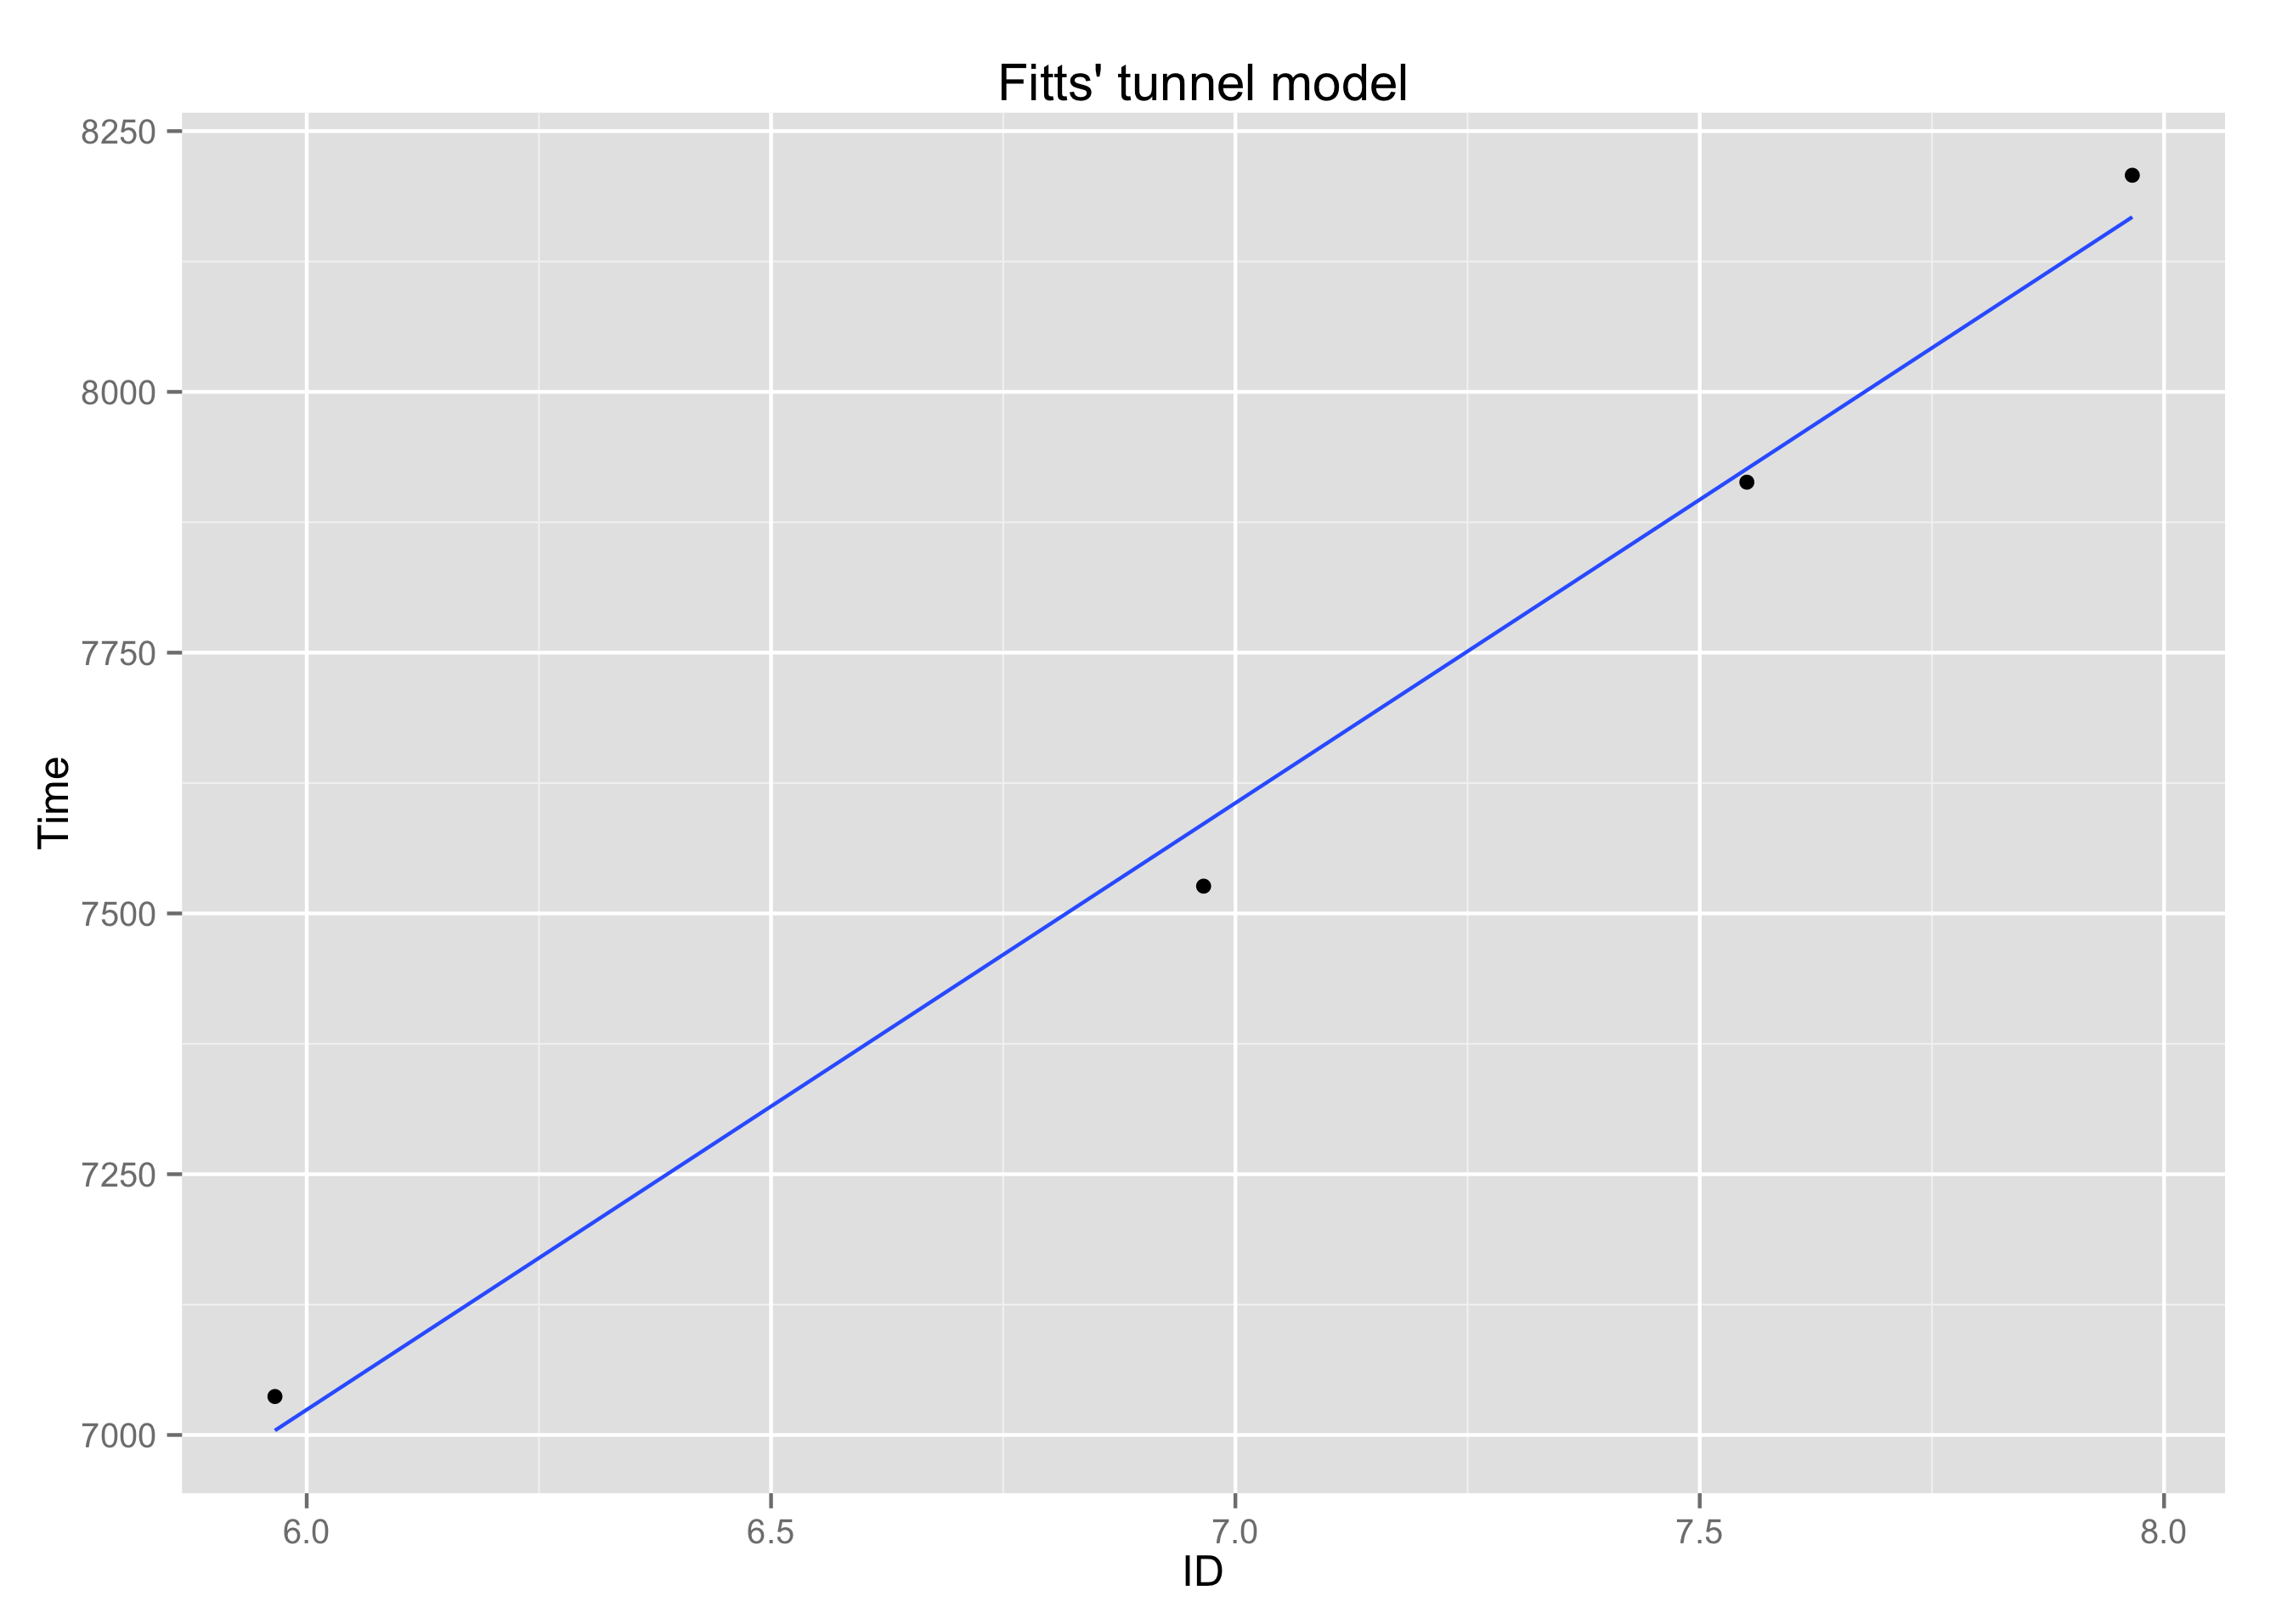
\includegraphics[width=\textwidth]{images/plots/plot_model_tunnel_fitt}
		\captionof{figure}{Fitts' affine model til gennemsnitstiden pr. $ID$, med $ID$ på $x$-aksen og tiden $T$ på $y$-aksen.}
		\label{fig:fitt_tunnel_line}
	\end{minipage}
\end{minipage}
\begin{minipage}{\linewidth}
	\begin{minipage}[t]{.45\linewidth}
		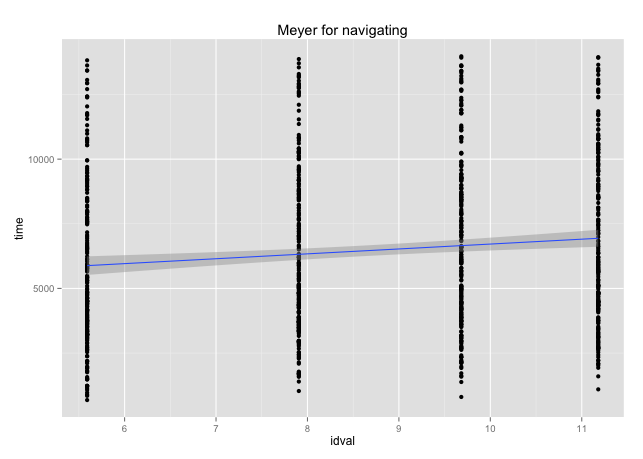
\includegraphics[width=\textwidth]{images/plots/plot_model_tunnel_meyer}
		\captionof{figure}{Meyer's affine model til gennemsnitstiden pr. $ID$, med $ID$ på $x$-aksen og tiden $T$ på $y$-aksen.}
		\label{fig:meyer_tunnel_line}
	\end{minipage}
	\begin{minipage}[b]{0.1\linewidth}
	~
	\end{minipage}
	\begin{minipage}[t]{0.45\linewidth}
		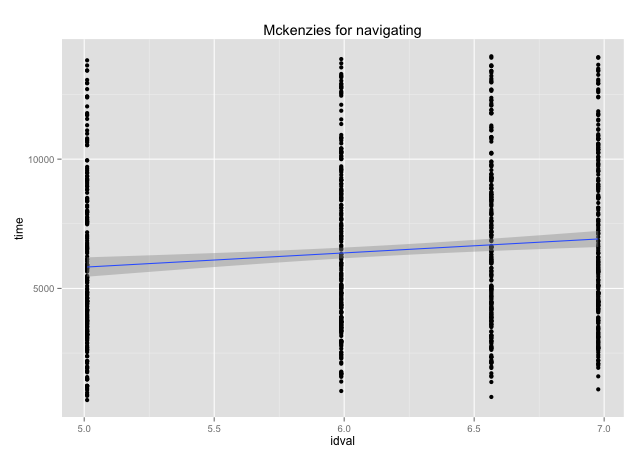
\includegraphics[width=\textwidth]{images/plots/plot_model_tunnel_mackenzie}
		\captionof{figure}{Mackenzie's affine model til gennemsnitstiden pr. $ID$, med $ID$ på $x$-aksen og tiden $T$ på $y$-aksen.}
		\label{fig:mackenzie_tunnel_line}
	\end{minipage}
\end{minipage}
\begin{minipage}{\linewidth}
	\begin{minipage}[t]{\linewidth}
		\centering
		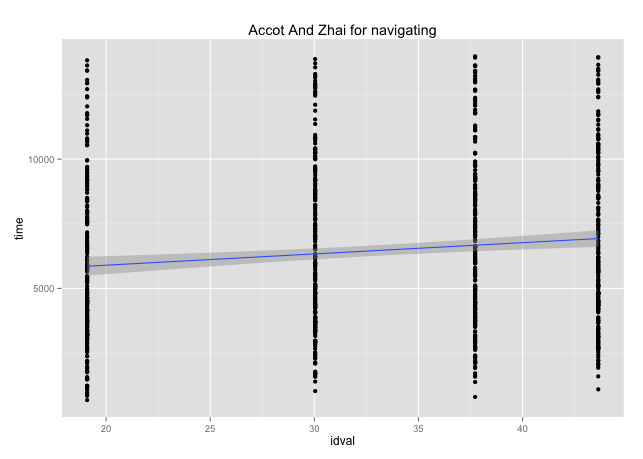
\includegraphics[width=0.5\textwidth]{images/plots/plot_model_tunnel_accot}
		\captionof{figure}{Accot \& Zhai's affine model til gennemsnitstiden pr. $ID$, med $ID$ på $x$-aksen og tiden $T$ på $y$-aksen.}
		\label{fig:accot_tunnel_line}
	\end{minipage}
\end{minipage}

\newpage
\addcontentsline{toc}{subsection}{Analyse af spiralopgaver}
\subsection*{Analyse af spiralopgaver}
For at kunne tilpasse vores fire originale formuleringer af Fiits' lov, har vi defineret afstanden af $A$ som længden på spiralens bane i pixels. Disse afstande er bestemt på baggrund af antal vindinger til $A = [127,190,252,315]$. Bredden på målet, $W$, har vi valgt som længden på den inderste vandrette linje i spiralen, slutstregen, som altid er 25 pixels bred. Ved disse værdier kan vi tilpasse formuleringernes tilhørende $ID$ og tiden $T$ per opgave til en lineær model, med $lm()$, for alle vores filtrerede og unkontrollerede datapunkter. De fire matematiske modelfremstillinger med respektive konstanter er vist nedenfor.
\begin{align*}
\text{Fitts': } &T = -24882.5+ 8217.7 \cdot \log_2\left(\frac{2A}{W}\right)\\
\text{Welford's: } &T =  2808.54\cdot \log_2\left(\frac{A+\frac{1}{2}W}{W}\right)\\
\text{Mackenzie's: } &T = -21606.0 + 9310.7\cdot \log_2\left(\frac{A+W}{W}\right)\\
\text{Meyer's: } &T = -16269.1 + 8452.2 \cdot \sqrt{\frac{A}{W}}
\end{align*}

Accot og Zhai argumenterer i \cite{accot1997} for, at $ID$ for en navigationsopgave med en spiral, kan findes ved at opdele den i delelementer baseret på vinklen $\theta$. Ved hvert delelement kan bredden, $w$, findes og alle delelementerne summeres ved et integral over vinklerne på baggrund af antal vindinger, $n$. Dette integral, vist nedenfor, giver i følge Accot og Zhai et $ID_s$, som er specifikt for denne type navigationsopgaver. 
\begin{align*}
ID_s = \int_{2\pi}^{2\pi(n+1)}\frac{\sqrt{\left(\theta+w\right)^6+9\left(\theta+w\right)4}}{\left(\theta+2\pi+2\right)^3-\left(\theta+w\right)^3}d\theta
\end{align*}
For vores spiralopgaver gjorde vi brug af $n=[1,2,3,4]$ og en bredde $w=[3.1,3.1,3.1,3.05]$. For hver testperson i vores kontrollerede eksperiment har vi tilpasset deres tid $T$ og de fire udregnede $ID_s$ med lineær regression. Figur \ref{fig:spiralingtest1} og \ref{fig:spiralingtest2} viser de affine modellers tilpasning til de fire datapunkter for hhv. testperson 2 og 10. Det kan bemærkes, hvordan kurven er monotont voksende, hvilket stemmer overens med forventningen om, at det tager længere tid at gennemføre en opgave, hvis sværhedsgraden, $ID$, bliver højere. Imodsætning til tunnelopgaven var der ingen af testpersonerne i den kontrollerede forsøg, som blev hurtigere ved sværere $ID$.

\begin{minipage}{\linewidth}
	\begin{minipage}[b]{.45\linewidth}
		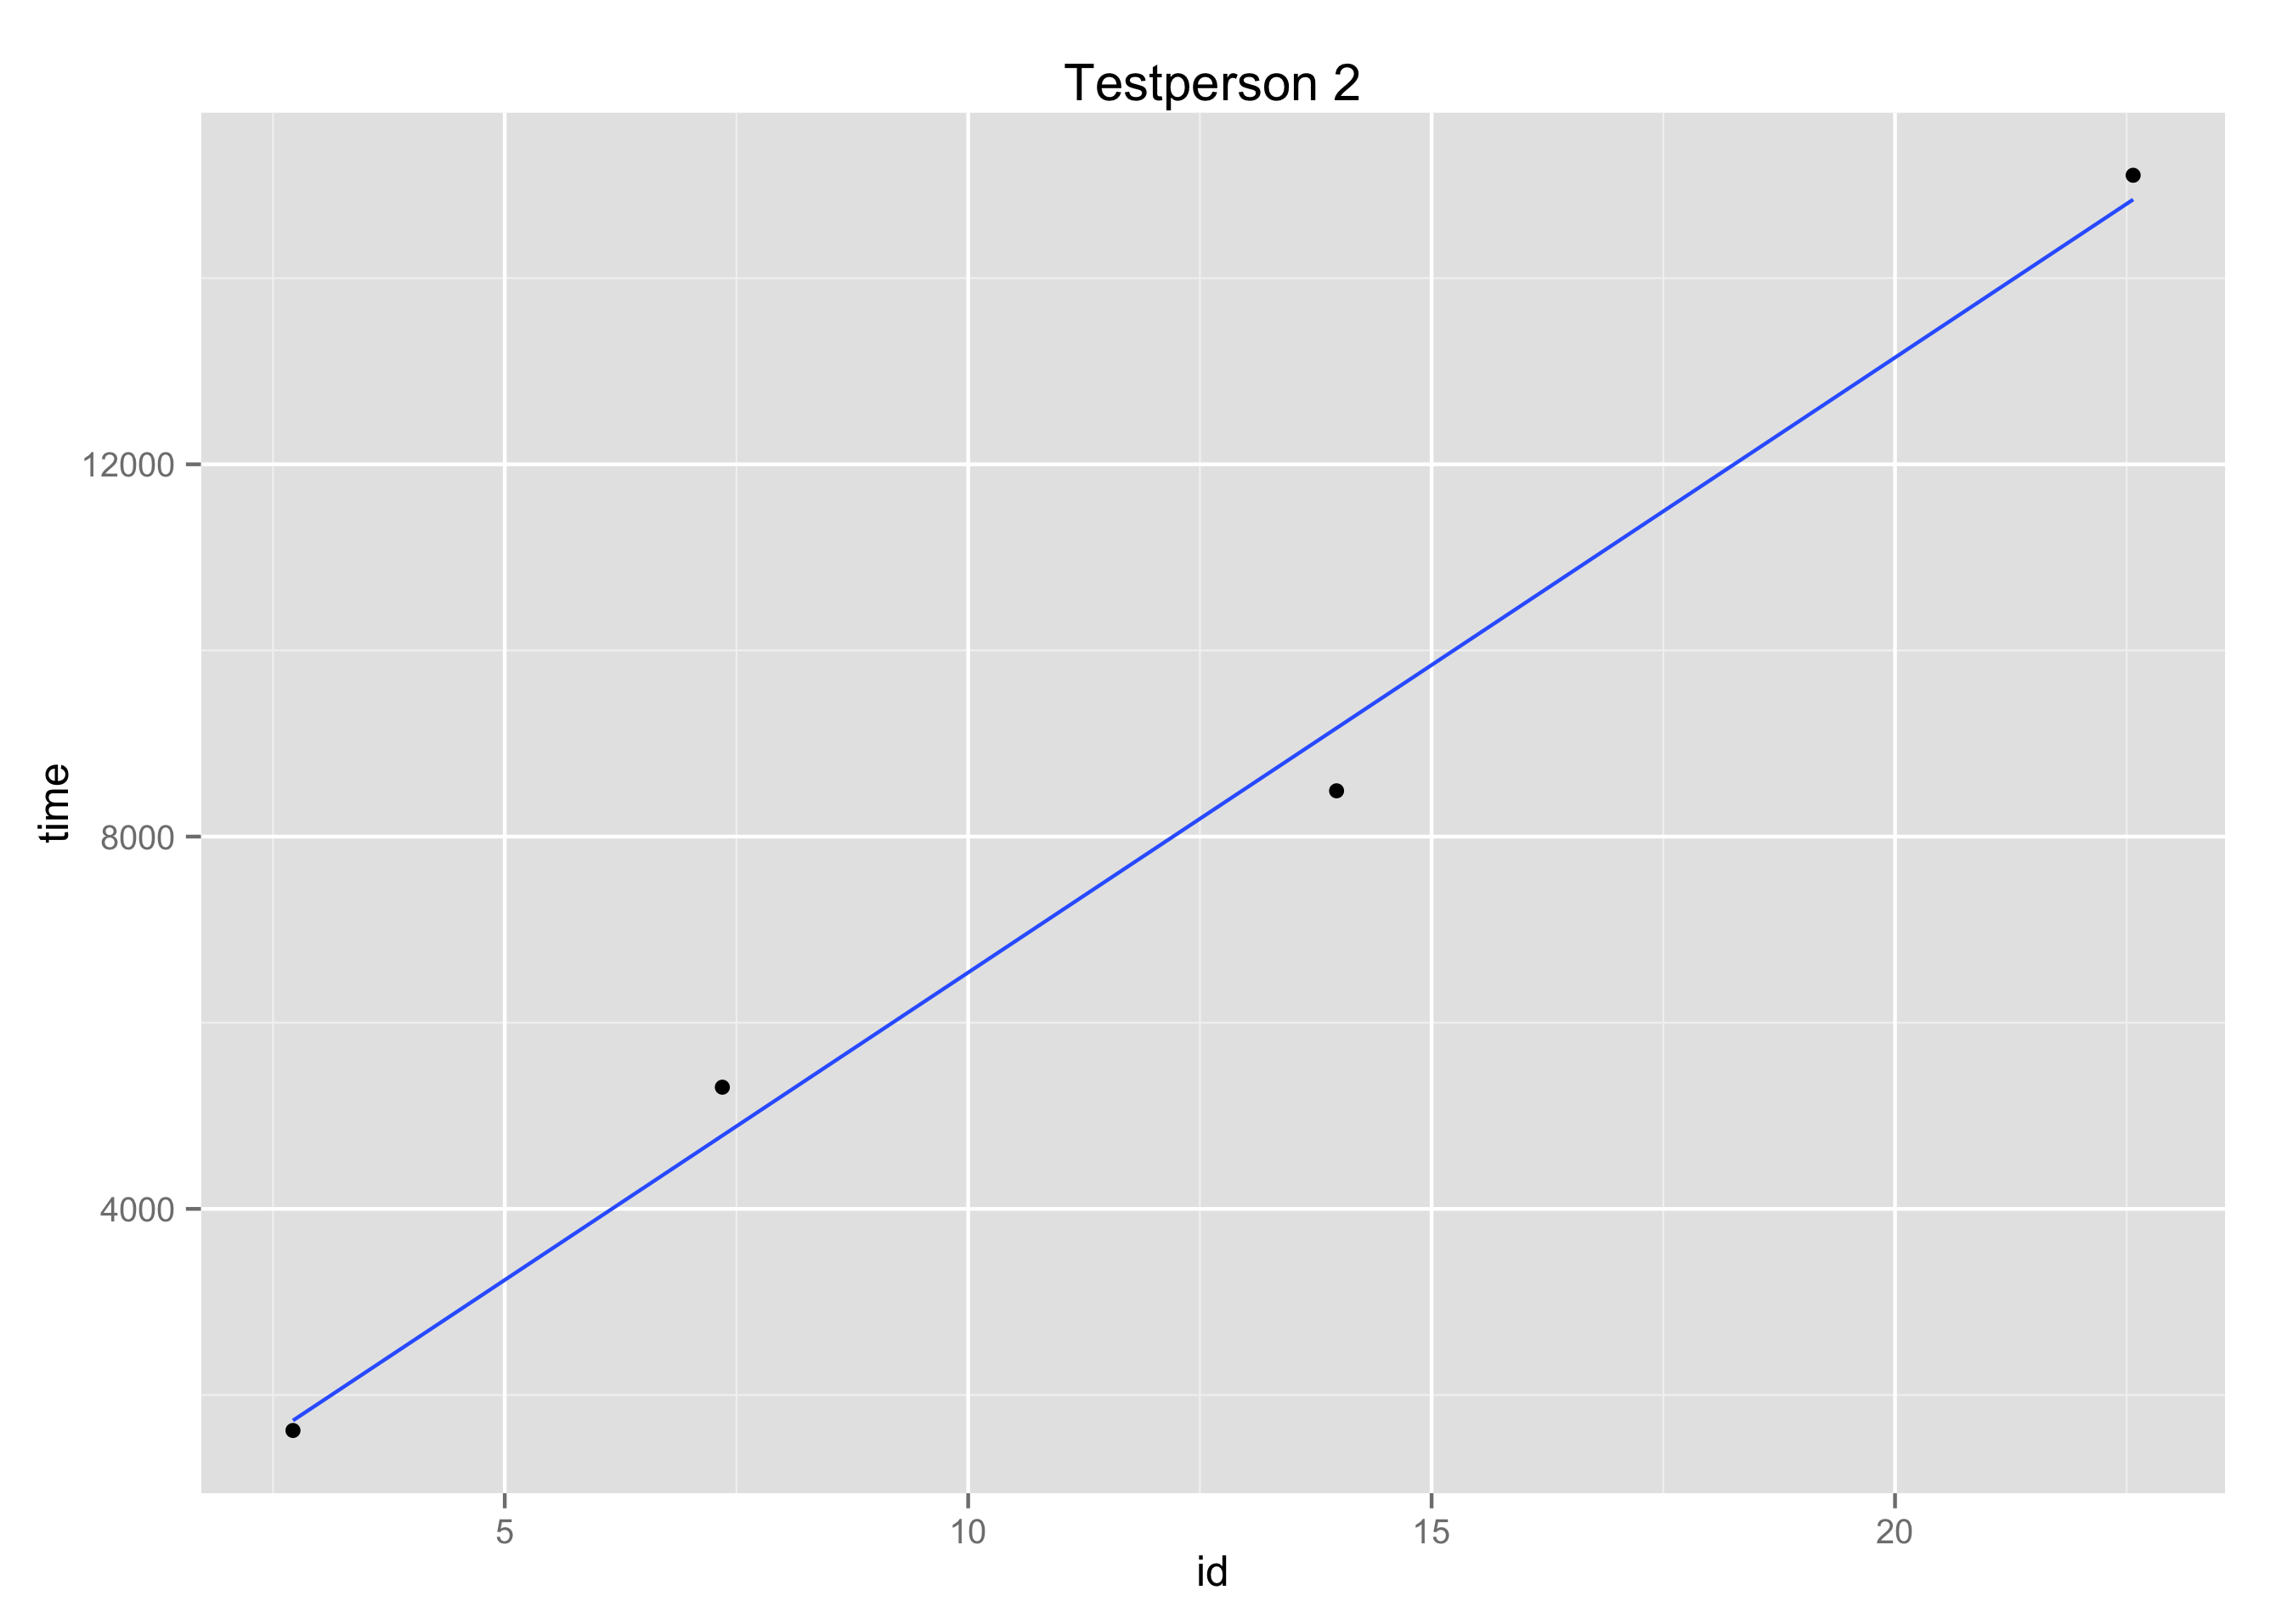
\includegraphics[width=\textwidth]{images/plots/plot_model_test_spiraling_1}
		\captionof{figure}{Accot og Zhai's formulering tilpasset til testperson 2, med $ID_s$ på $x$-aksen og tiden $T$ på $y$-aksen.}
		\label{fig:spiralingtest1}
	\end{minipage}
	\begin{minipage}[b]{0.1\linewidth}
	~
	\end{minipage}
	\begin{minipage}[b]{0.45\linewidth}
		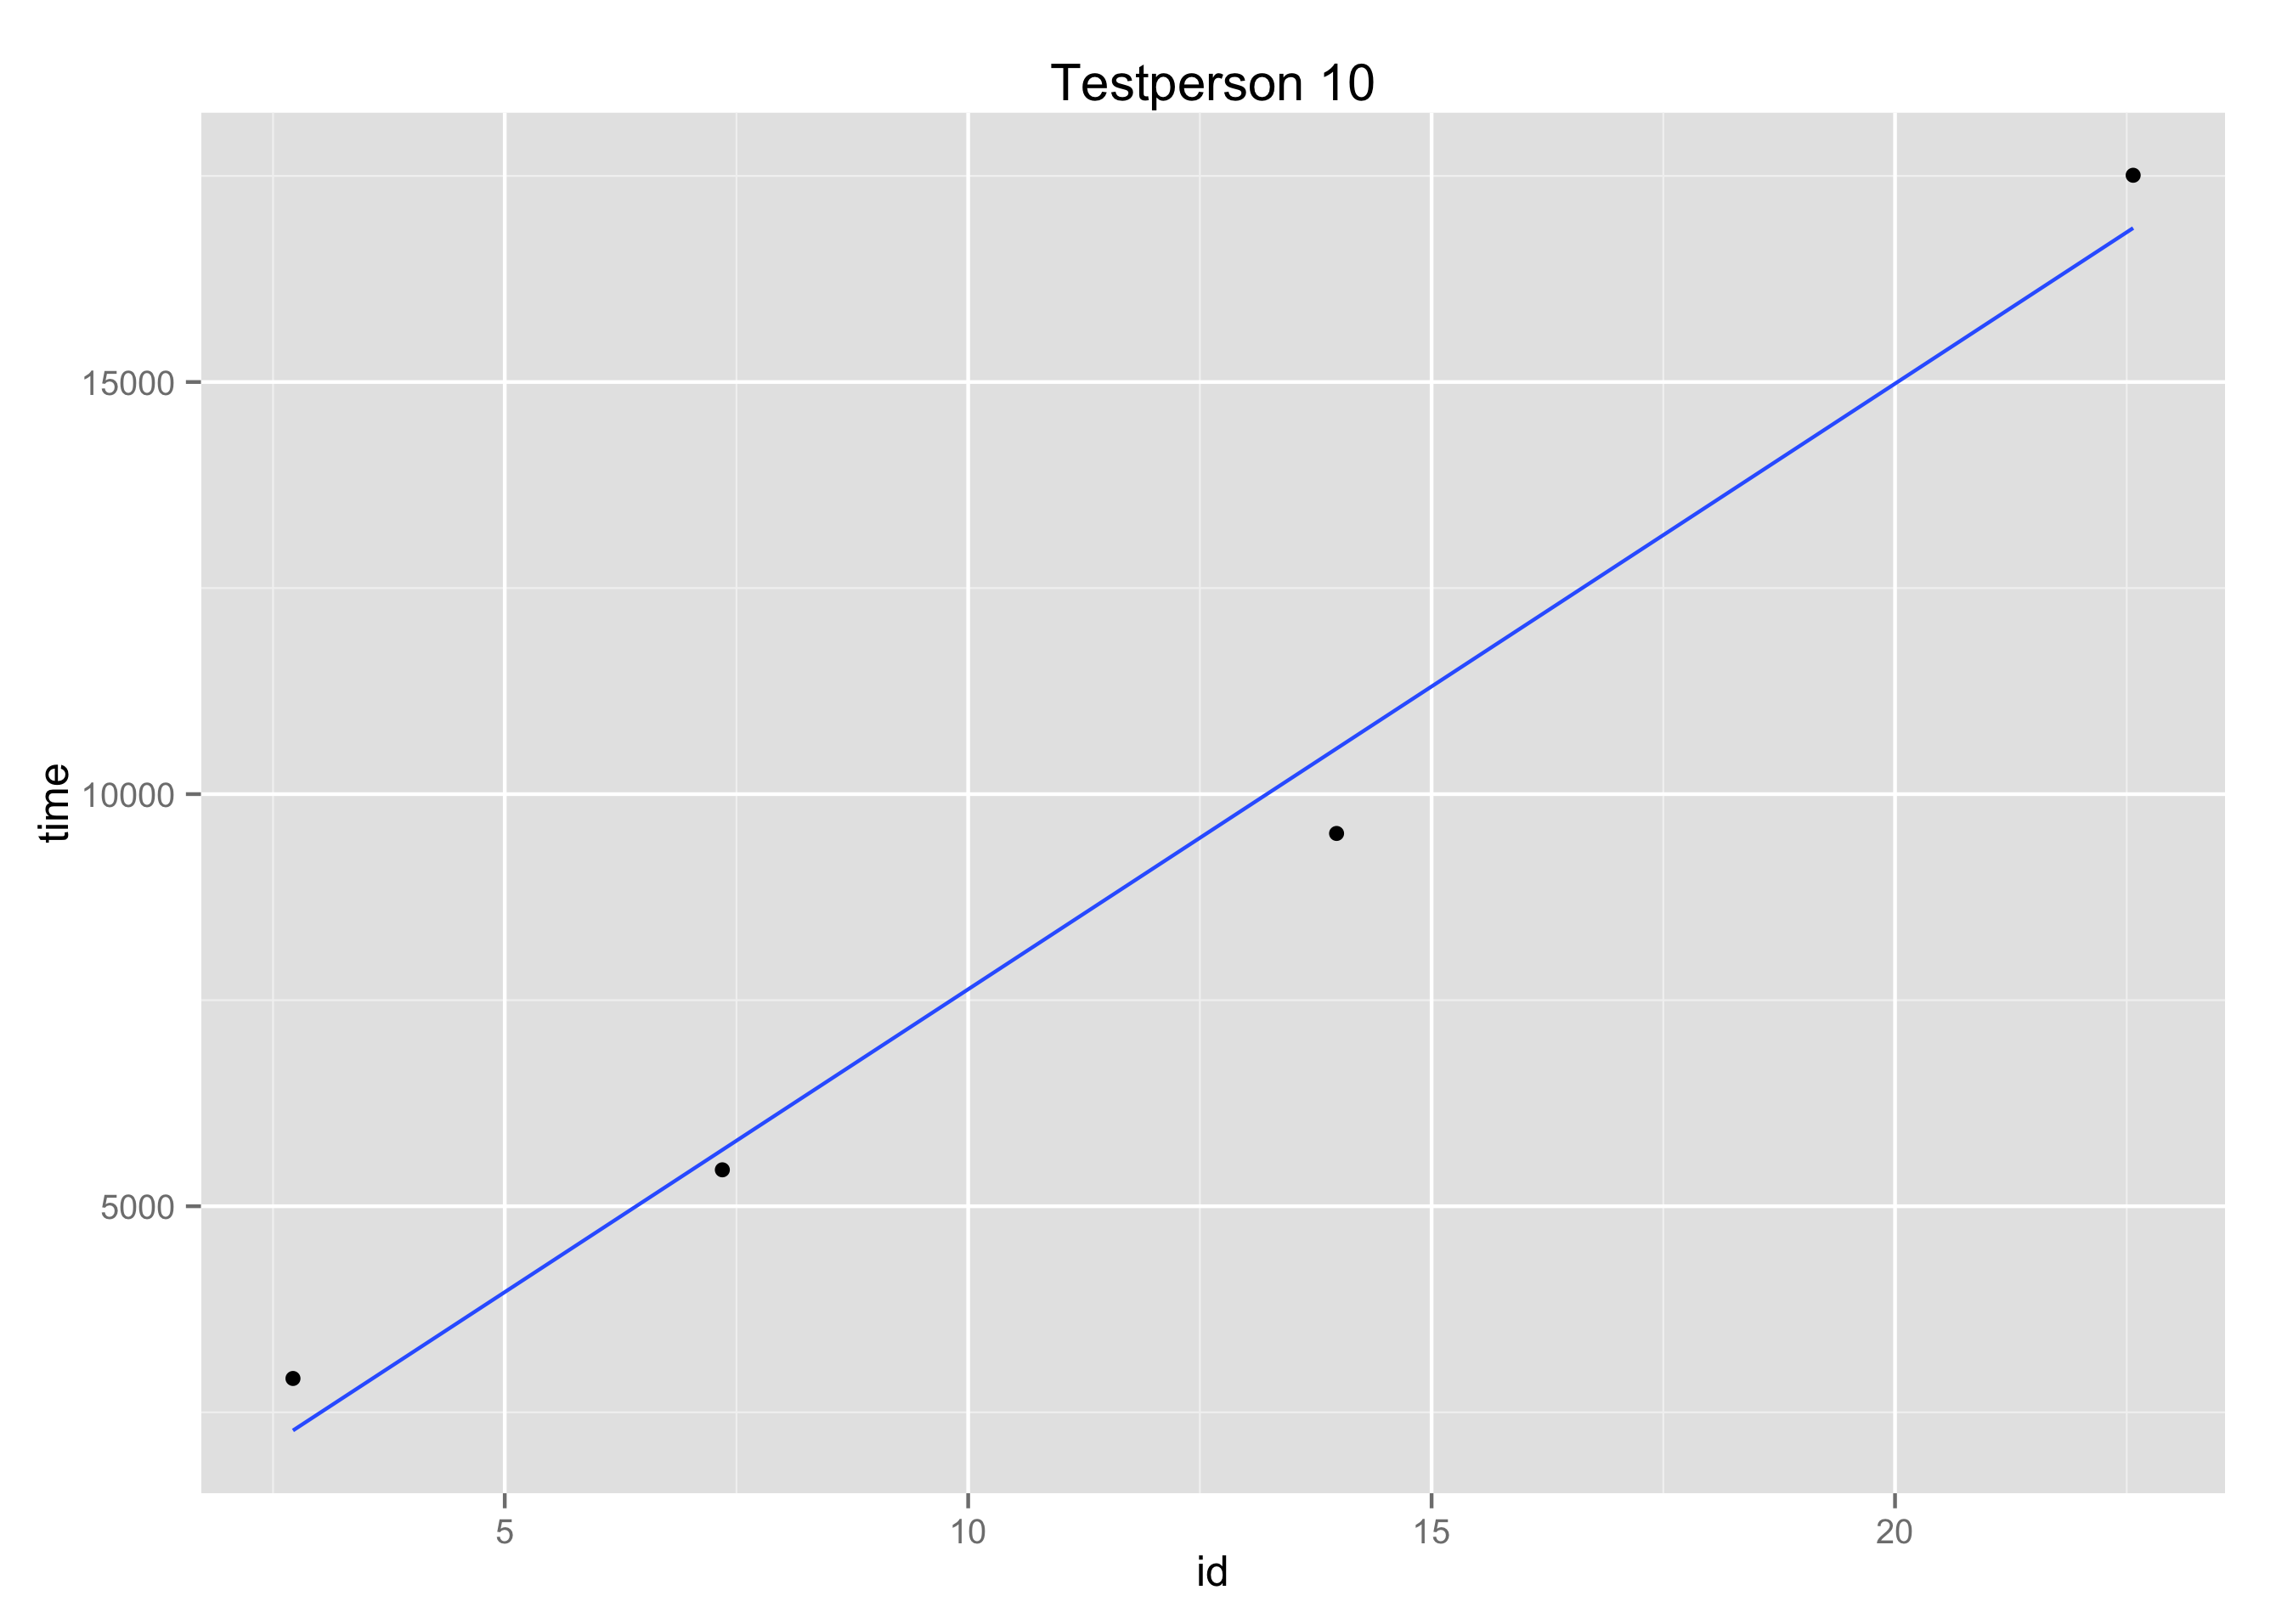
\includegraphics[width=\textwidth]{images/plots/plot_model_test_spiraling_2}
		\captionof{figure}{Accot og Zhai's formulering tilpasset til testperson 10, med $ID_s$ på $x$-aksen og tiden $T$ på $y$-aksen.}
		\label{fig:spiralingtest2}
	\end{minipage}
\end{minipage}

\newpage
Ved at tilpasse Accot og Zhai's $ID$ til vores filtrerede og ukontrollerede datapunkter fandt vi frem til den matematiske model i ligning \ref{eq:accotspiral}. Det kan bemærkes, at de to konstante led for denne model er markant anderledes end de tilsvarende for de fire andre formuleringer.  AIC analysen i tabel \ref{tab:table_analysis_aic_spiral} viser, hvordan Accot og Zhai's formulering klarer sig væsentligt bedre end de fire andre. Dette er også, hvad vi forventede, da de formuleringer ikke er beregnet til denne type navigationsopgaver.
\begin{align}
\text{Accot \& Zhai: } T = 2097.09+553.25 \cdot \int_{2\pi}^{2\pi(n+1)}\frac{\sqrt{\left(\theta+w\right)^6+9\left(\theta+w\right)4}}{\left(\theta+2\pi+2\right)^3-\left(\theta+w\right)^3}d\theta
\label{eq:accotspiral}
\end{align}

For at visualisere de fem modellers tilpasning til data, har vi taget gennemsnittet af tiden pr. $ID$ og tilpasset de fem formuleringer hertil. De tilsvarende fem affine kurver og datapunkter kan ses i figur \ref{fig:welford_spiral_line}-\ref{fig:accot_spiral_line}.

\begin{table}[h]
\centering
\begin{tabular}{lll}
Model & AIC værdi & Forskel\\\hline
Accot \& Zhai & 20225.67 & 0\\
Meyer & 20240.39 & 14.72 \\
Mackenzie & 20256.62 & 30.95\\
Welford & 20259.13 & 33.46\\
Fitts & 20262.07 & 36.4
\end{tabular}
\caption{AIC værdier og indbyrdes forskel med udgangspunkt i Fitts' som nulpunkt}
\label{tab:table_analysis_aic_spiral}
\end{table}

\begin{minipage}{\linewidth}
	\begin{minipage}[t]{.45\linewidth}
		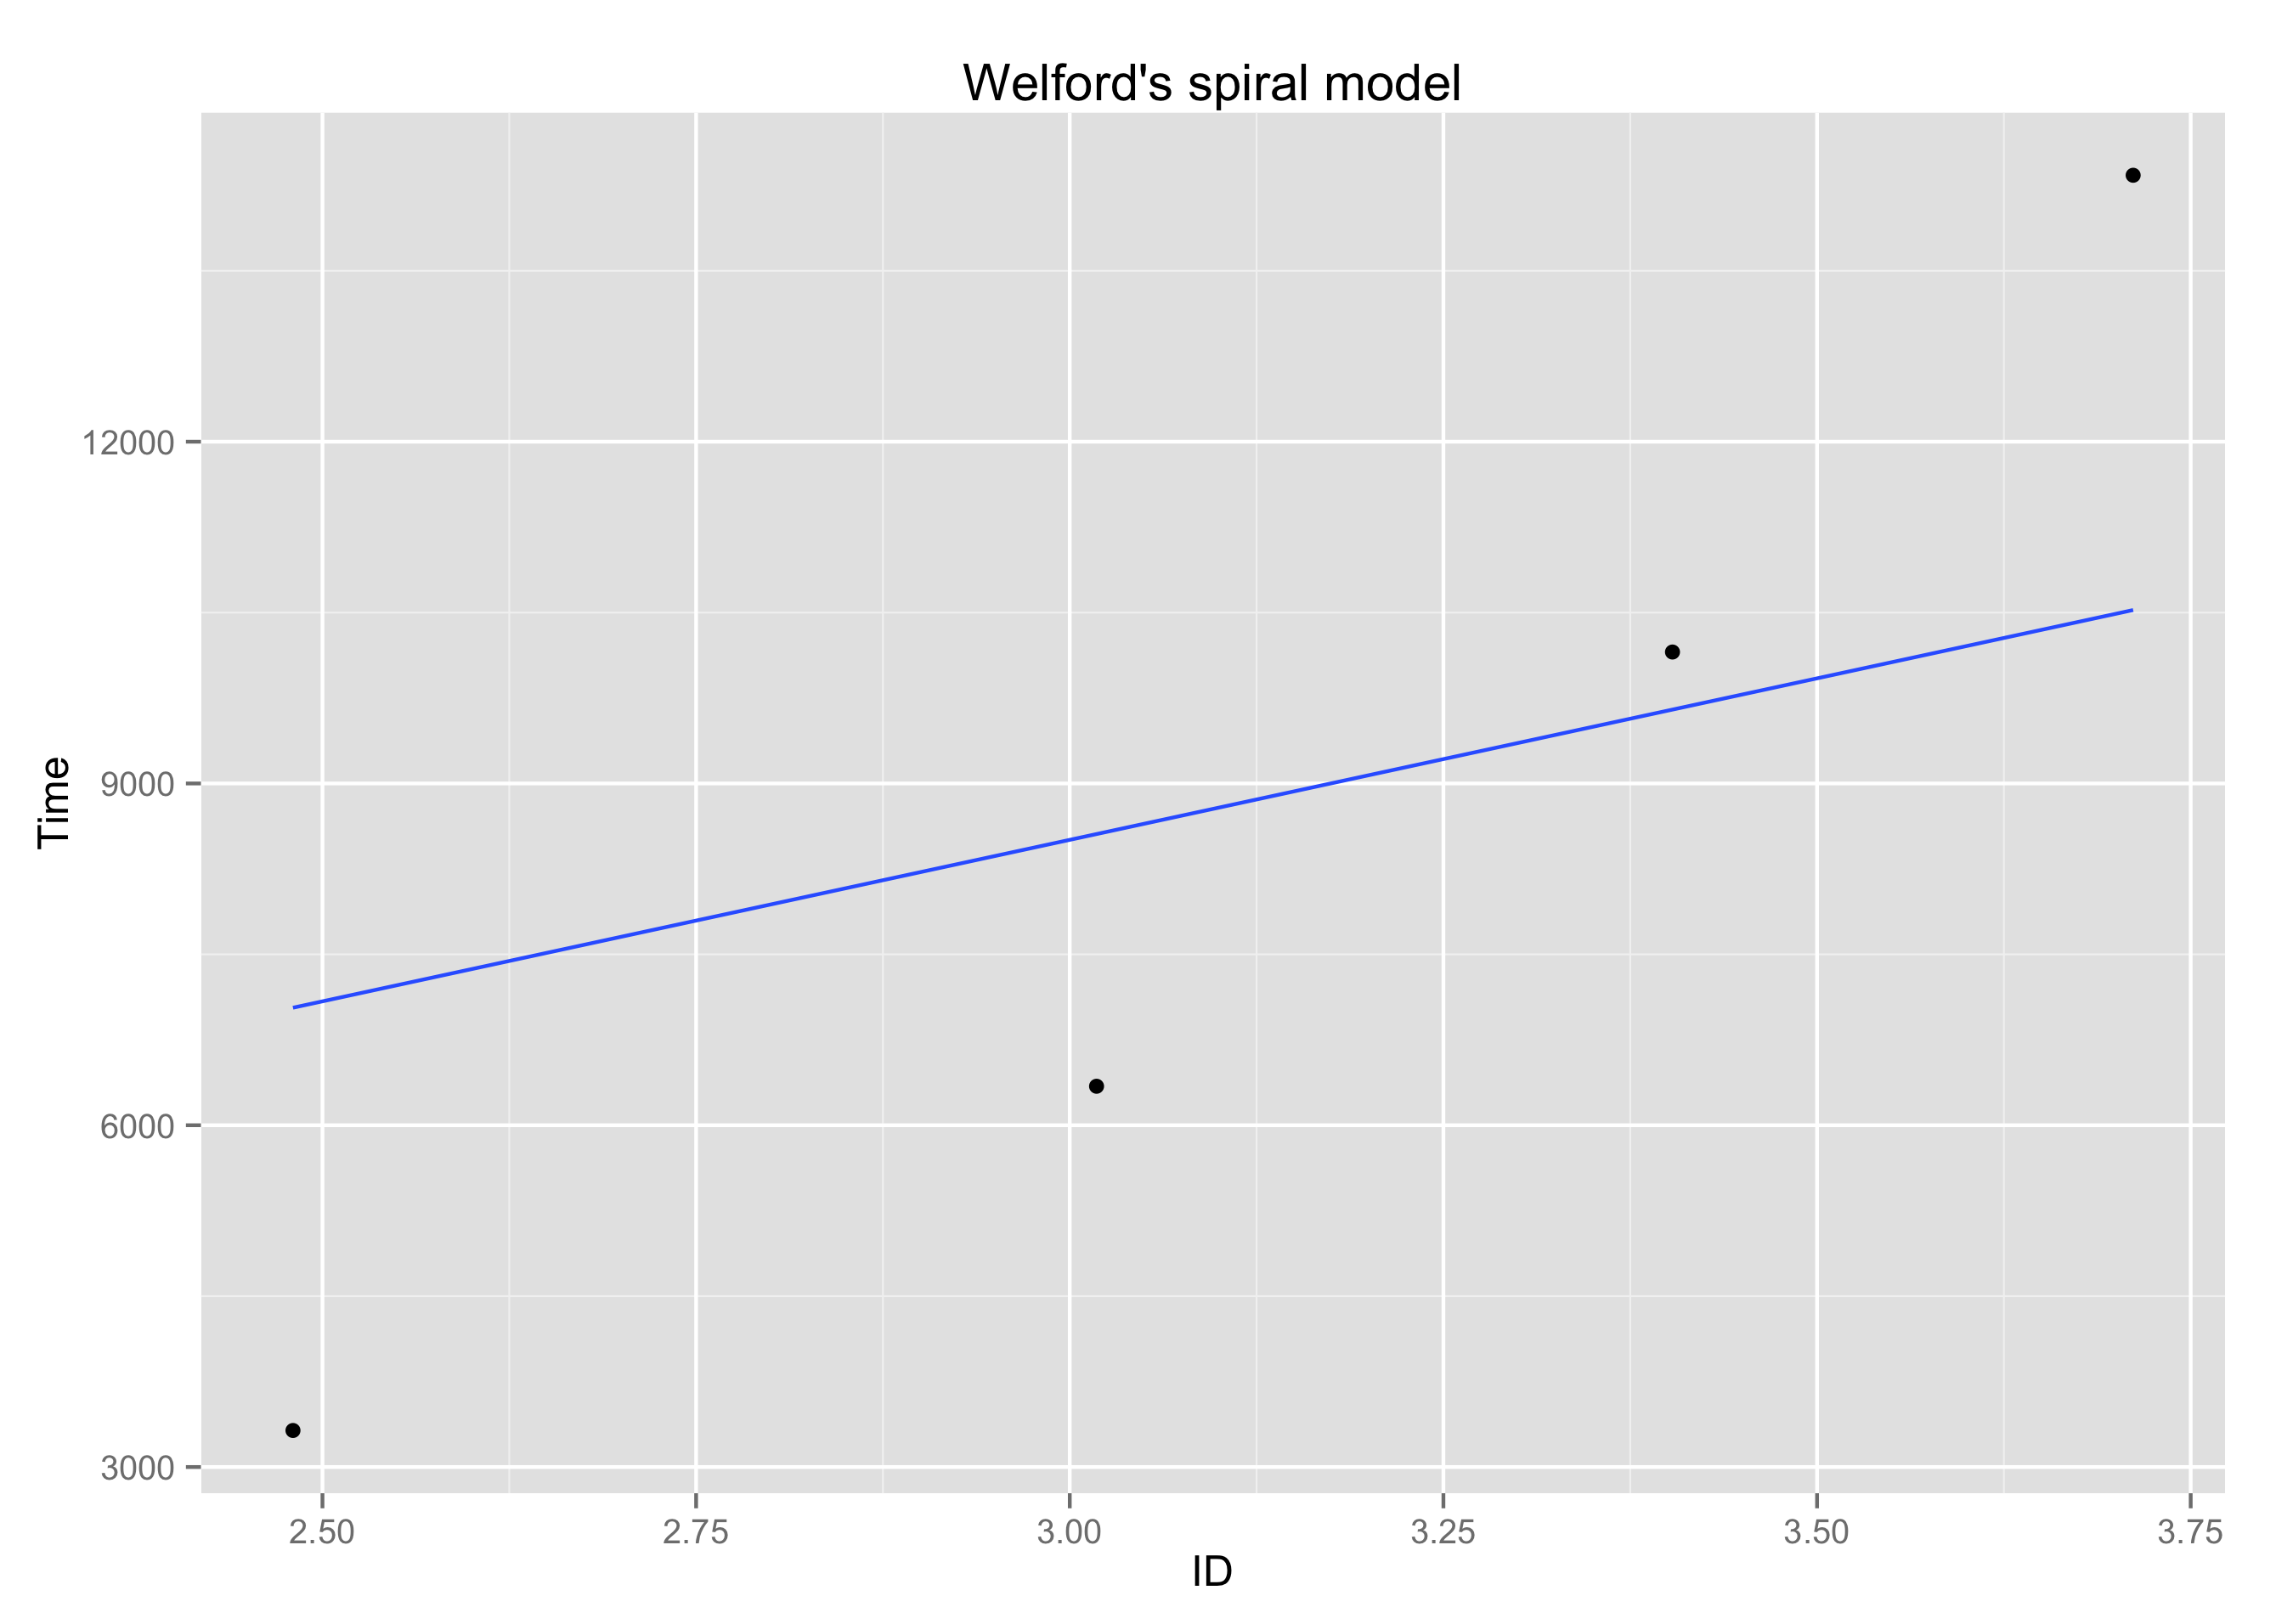
\includegraphics[width=\textwidth]{images/plots/plot_model_spiral_welford}
		\captionof{figure}{Welford's affine model til gennemsnitstiden pr. $ID$, med $ID$ på $x$-aksen og tiden $T$ på $y$-aksen.}
		\label{fig:welford_spiral_line}
	\end{minipage}
	\begin{minipage}[b]{0.1\linewidth}
	~
	\end{minipage}
	\begin{minipage}[t]{0.45\linewidth}
		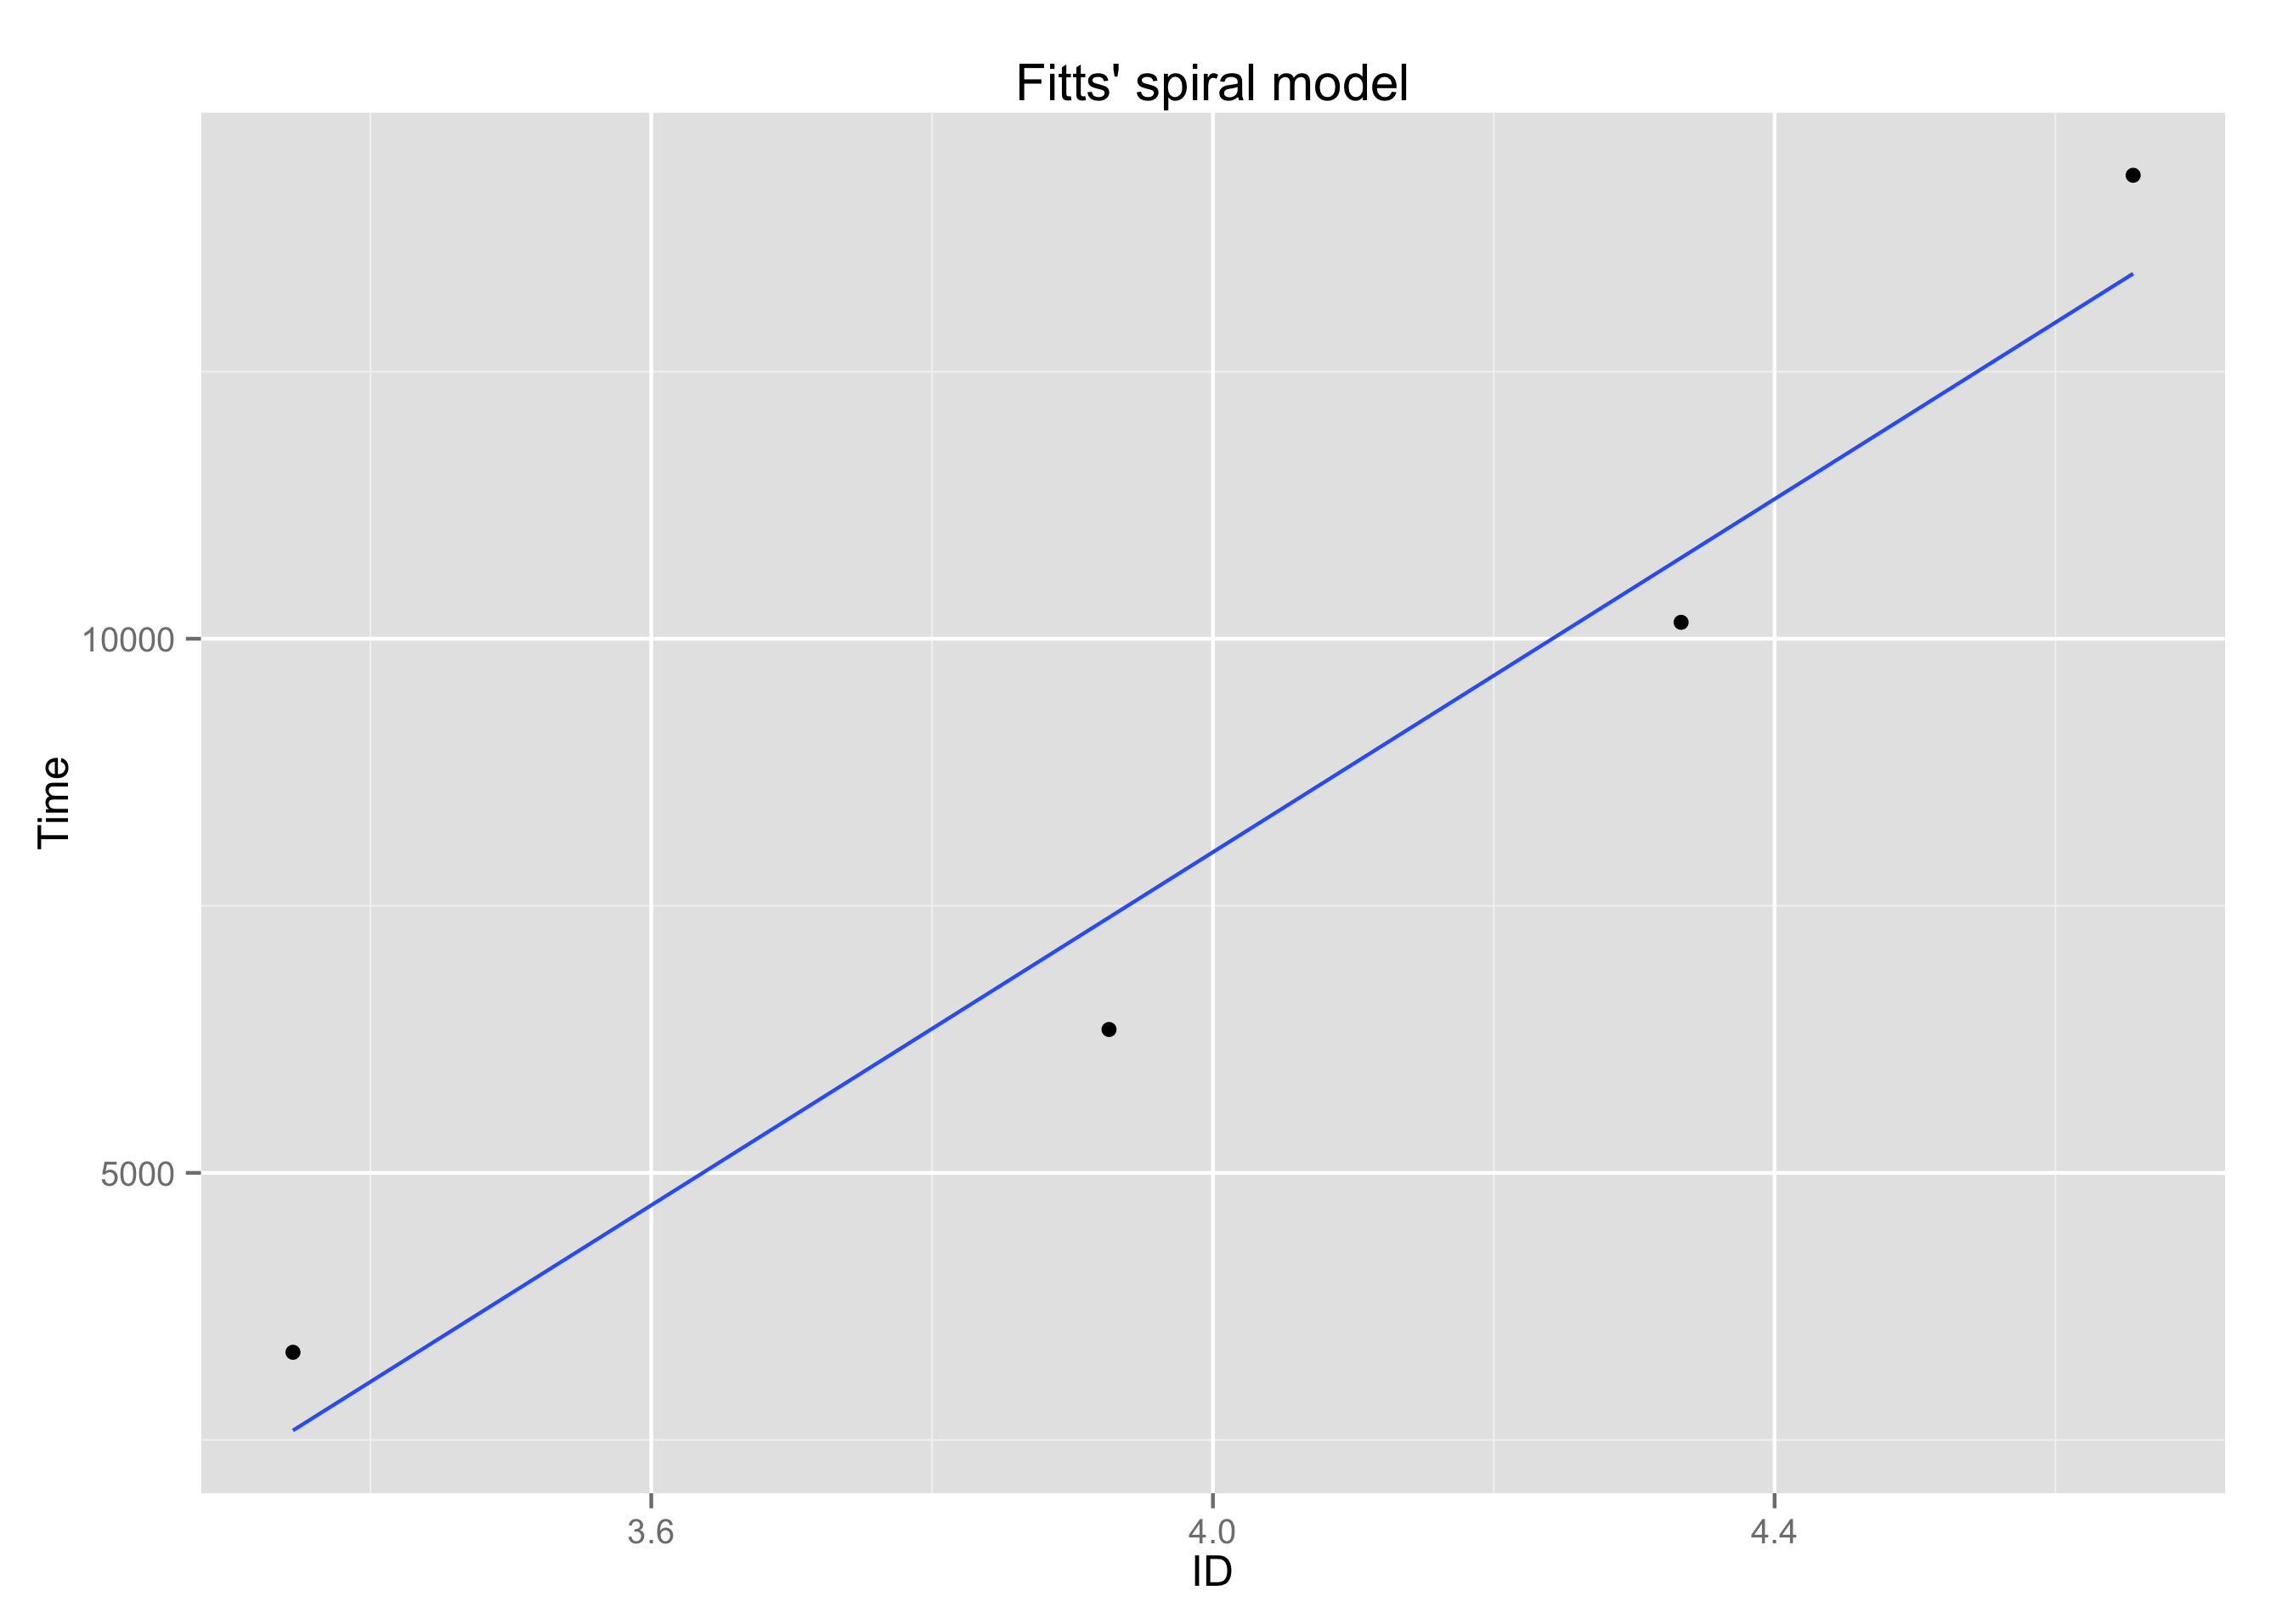
\includegraphics[width=\textwidth]{images/plots/plot_model_spiral_fitt}
		\captionof{figure}{Fitts' affine model til gennemsnitstiden pr. $ID$, med $ID$ på $x$-aksen og tiden $T$ på $y$-aksen.}
		\label{fig:fitt_spiral_line}
	\end{minipage}
\end{minipage}
\begin{minipage}{\linewidth}
	\begin{minipage}[t]{.45\linewidth}
		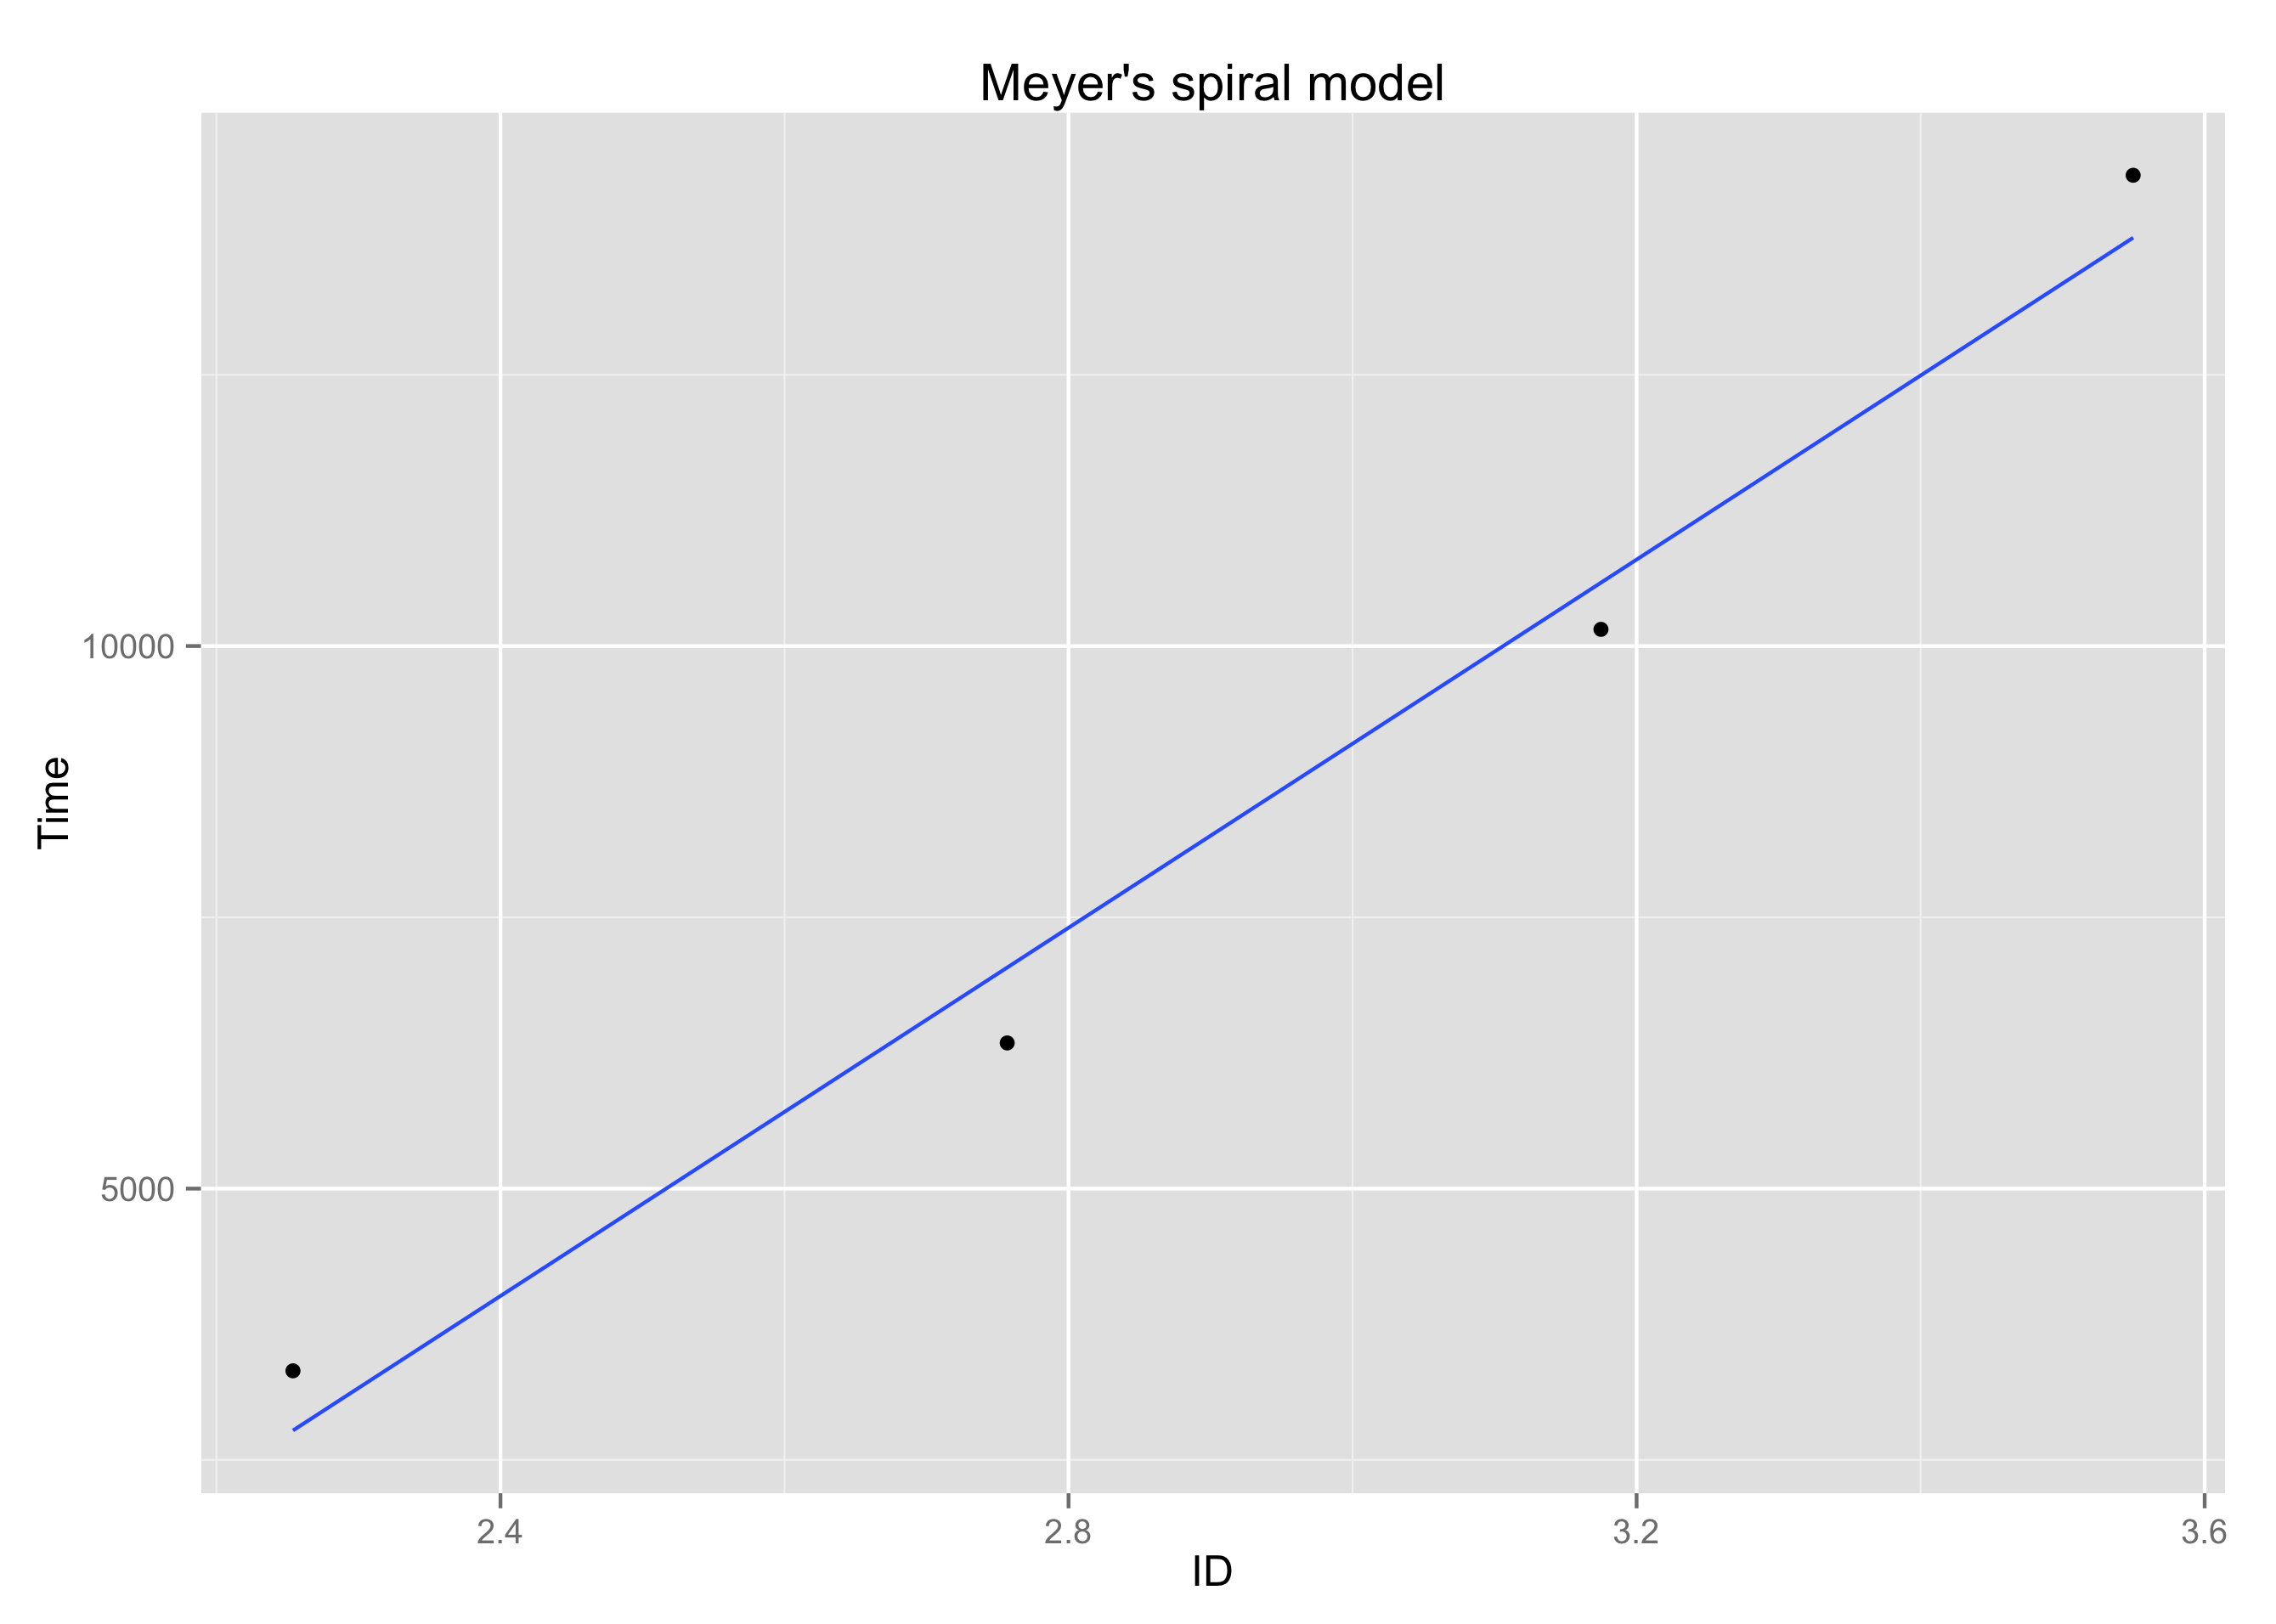
\includegraphics[width=\textwidth]{images/plots/plot_model_spiral_meyer}
		\captionof{figure}{Meyer's affine model til gennemsnitstiden pr. $ID$, med $ID$ på $x$-aksen og tiden $T$ på $y$-aksen.}
		\label{fig:meyer_spiral_line}
	\end{minipage}
	\begin{minipage}[b]{0.1\linewidth}
	~
	\end{minipage}
	\begin{minipage}[t]{0.45\linewidth}
		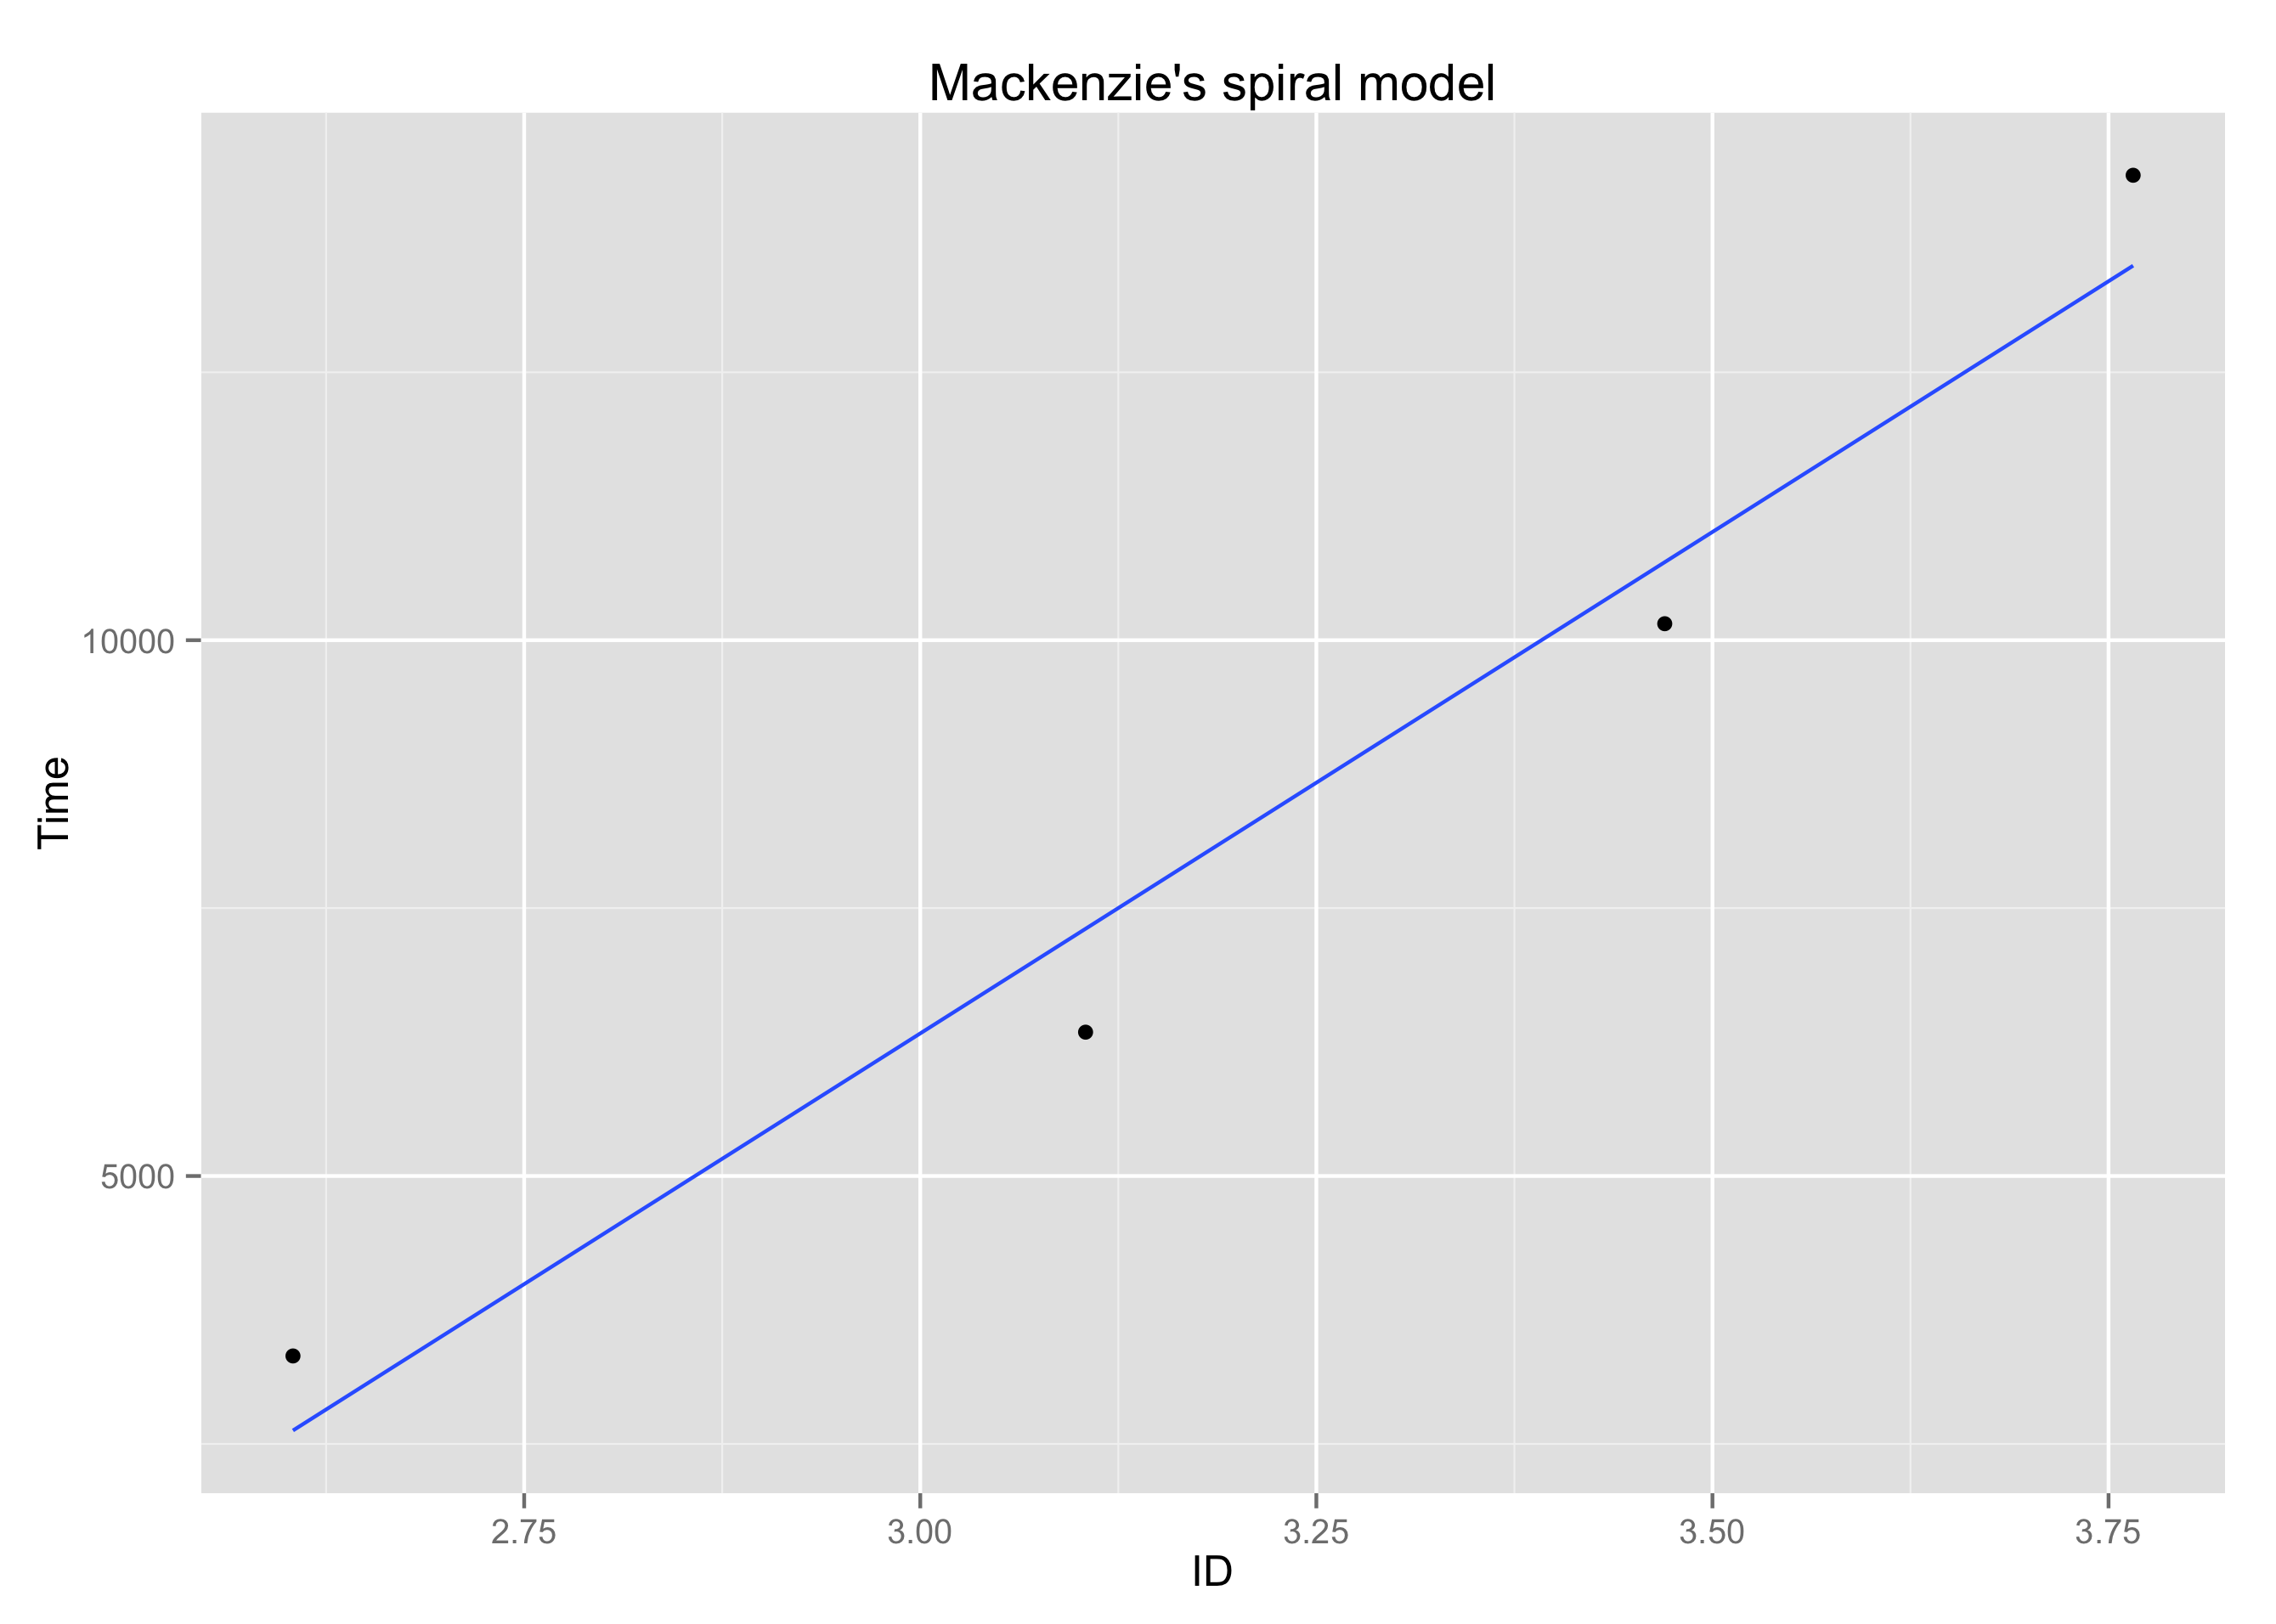
\includegraphics[width=\textwidth]{images/plots/plot_model_spiral_mackenzie}
		\captionof{figure}{Mackenzie's affine model til gennemsnitstiden pr. $ID$, med $ID$ på $x$-aksen og tiden $T$ på $y$-aksen.}
		\label{fig:mackenzie_spiral_line}
	\end{minipage}
\end{minipage}
\begin{minipage}{\linewidth}
	\begin{minipage}[t]{\linewidth}
		\centering
		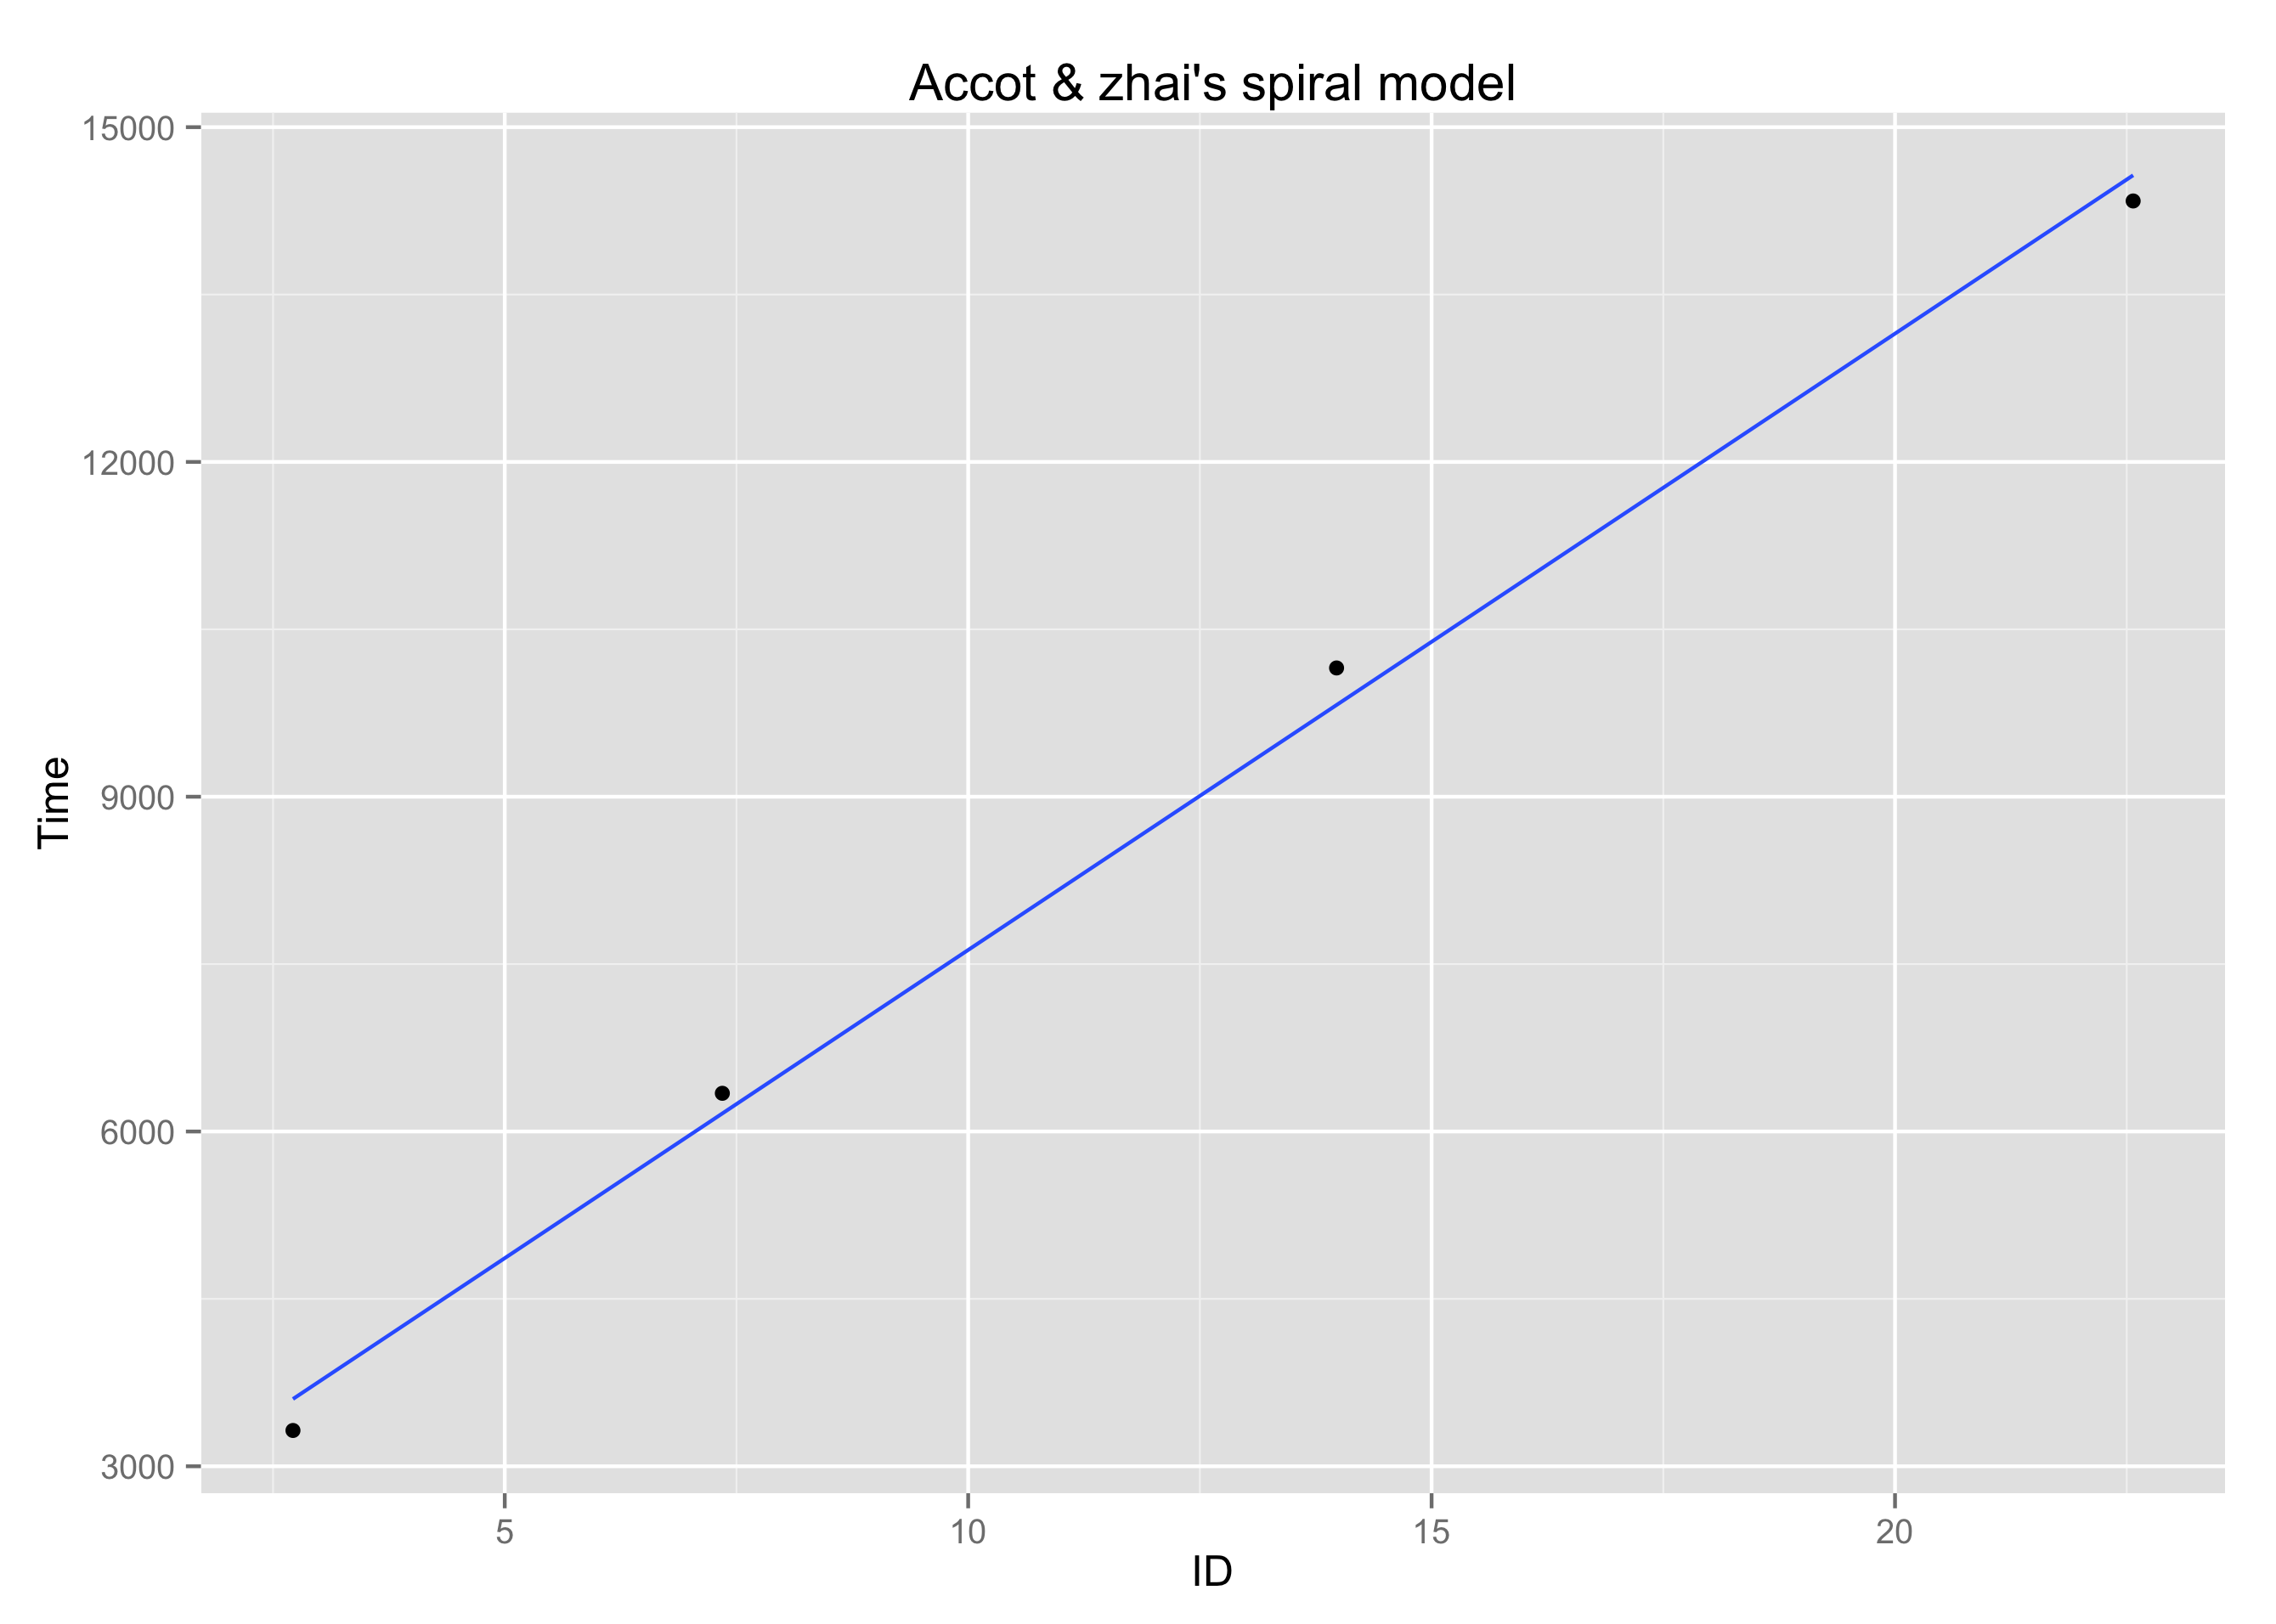
\includegraphics[width=0.5\textwidth]{images/plots/plot_model_spiral_accot}
		\captionof{figure}{Accot \& Zhai's affine model til gennemsnitstiden pr. $ID$, med $ID$ på $x$-aksen og tiden $T$ på $y$-aksen.}
		\label{fig:accot_spiral_line}
	\end{minipage}
\end{minipage}

\newpage
\addcontentsline{toc}{section}{Modelanalyse af hastighedsprofiler}
\section*{Modelanalyse af hastighedsprofiler}
Vores modelanalyse af hastighedsprofiler tager udgangspunkt i en kvantitativ og en kvalitativ analyse af de indsamlede hastighedsprofiler fra crowdsourcingdeltagernes pegeopgaver.

\begin{table}[h]
	\centering
	\begin{tabular}{llllll}
		Alder           & Køn               & Computerspil              & Computere                 & Hånd                & Pegeenhed            \\\hline
		gns: \hfill24.5 & mand: \hfill88\%  & $<1$ time: \hfill24\%     & $<1$ time: \hfill2\%      & venstre: \hfill14\% & mus: \hfill61\%      \\
		min: \hfill13   & kvinde: \hfill9\% & $1-5$ timer: \hfill24\%   & $1-5$ timer: \hfill1\%    & højre: \hfill83\%   & touchpad: \hfill36\% \\
		max: \hfill62   & andet: \hfill3\%  & $5-15$ timer: \hfill27\%  & $5-15$ timer: \hfill2\%   & andet: \hfill3\%    & andet: \hfill3\%     \\
		                &                   & $15-40$ timer: \hfill22\% & $15-40$ timer: \hfill24\% &                     &\\
		                &                   & $>40$ timer: \hfill3\%    & $>40$ timer: \hfill71\%   &                     &
	\end{tabular}
	\caption{TODO: Tabel med oversigt over gennemsnitsværdier og fordeling af testpersoners valg i spørgeskemaet.}
	\label{tab:persons_average}
\end{table}

\addcontentsline{toc}{subsection}{Kvalitativ analyse}
\subsection*{Kvalitativ analyse}
Vi har valgt at udføre en kvalitativ analyse af bevægelsesbanerne, da det vil give os et større overblik over den indsamlede data og vise os hvilke tendenser der kan observeres.
Den kvalitative analyse bygger på 57 tilfældigt crowdsourcingdeltagerne, hvilket svarer til cirka $21\%$ af deltagerne. Af de 57 deltagere angav 32 at de brugte mus, mens 25 angav at deres pegeredskab var touchpad. Vores observationer baserer sig på bevægelsesbanerne for hver deltager, et eksempel herpå ses i figur \ref{fig:movement_random_person}.

Vi har observeret at deltagerne tager en stor underbevægelse, eventuelt opfulgt af mindre korrigerende underbevægelser. Typisk vil der for muse-brugerne være en korrigerende underbevægelse, mens touchpad-brugerne ofte bruger flere korrigerende underbevægelser. Generelt har muse-brugerne også mindre udsving i deres bevægelsesbaner end touchpad-brugerne. Dertil var der flere deltagere som startede enkelte baner, med at bevæge pegeredskabet i en forkert retning.

\begin{minipage}{\linewidth}
	\begin{minipage}{.45\linewidth}
		\centering
		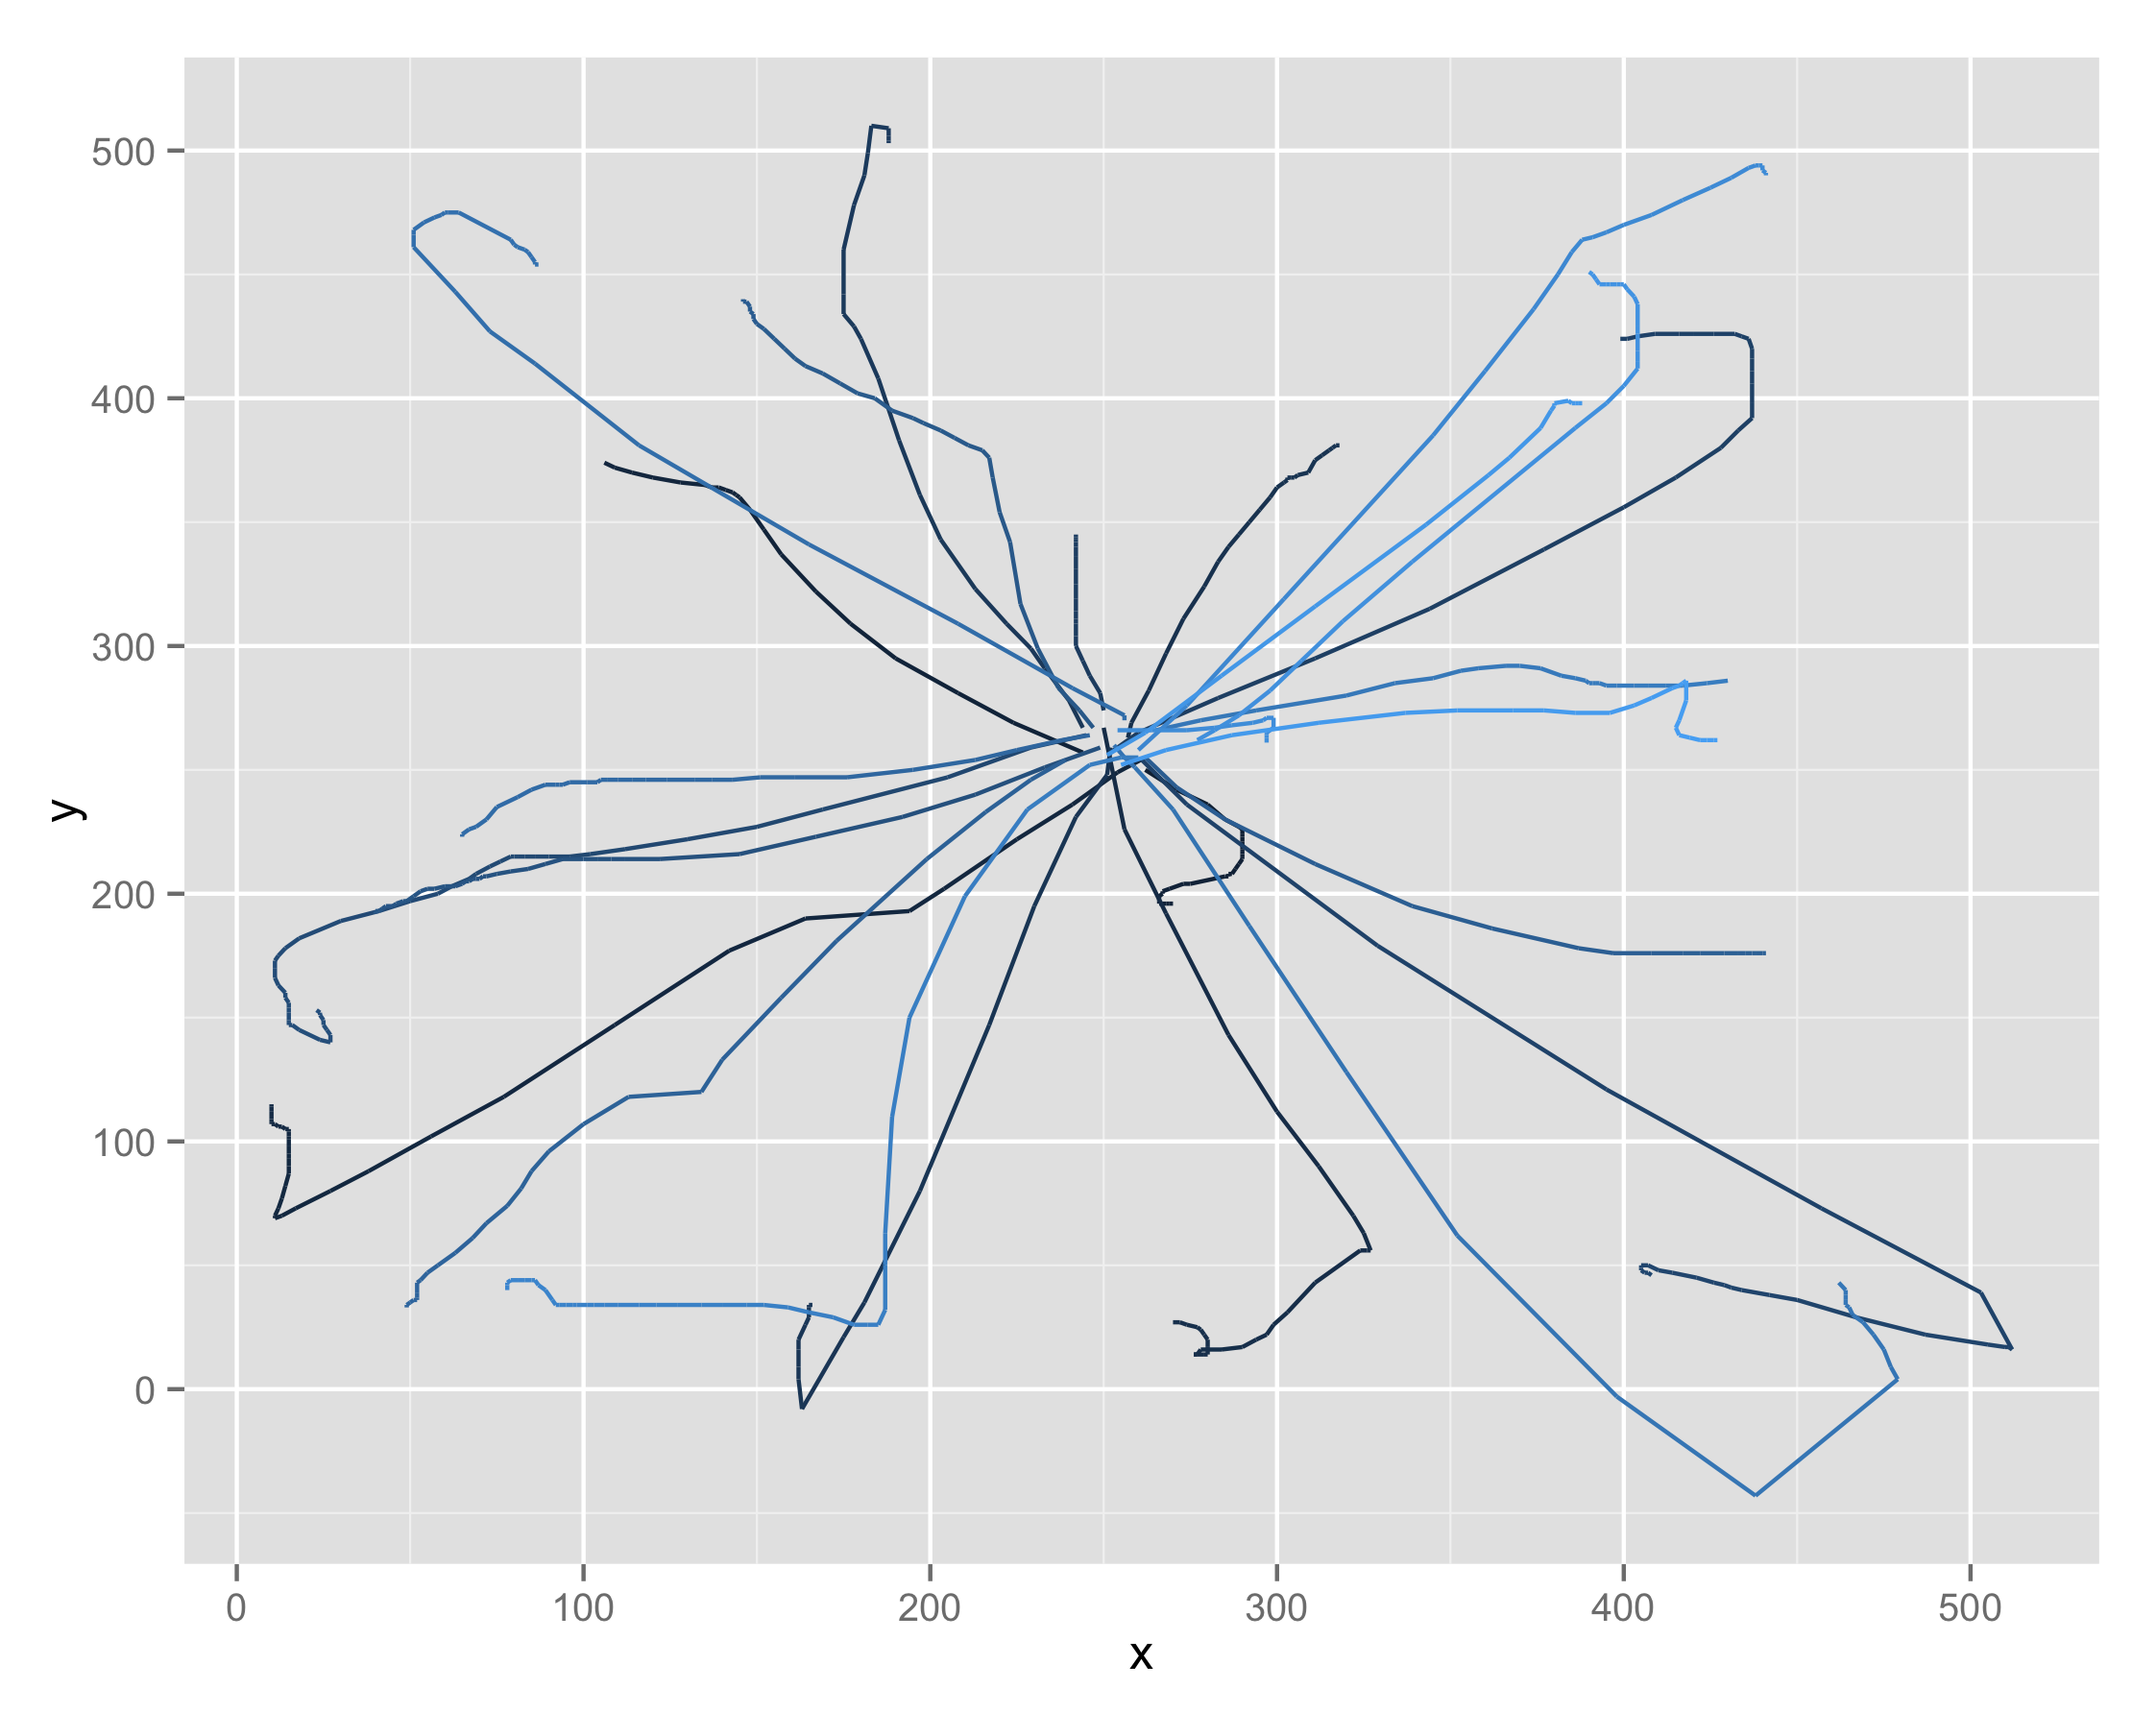
\includegraphics[width=\linewidth]{images/plots/plot_analysis_qualitative}
		\captionof{figure}{Plot over alle bevægelsesbaner lavet af en enkelt testdeltager under udførslen af denne deltagers pegeopgaver.}
		\label{fig:movement_random_person}
	\end{minipage}
	\begin{minipage}[b]{0.1\linewidth}
	~
	\end{minipage}
	\begin{minipage}{.45\linewidth}
		\centering
		\includegraphics[width=\linewidth]{images/plots/plot_speed_individual}
		\captionof{figure}{Fire plots over fartprofilerne for fire tilfældige pegeopgaver fra en tilfældig testdeltager}
		\label{fig:plot_speed_overall}
	\end{minipage}
\end{minipage}

\addcontentsline{toc}{subsection}{Kvantitativ analyse}
\subsection*{Kvantitativ analyse}
For at kunne analysere de indsamlede data, har vi valgt at lave nogle beregninger på vores data som kan bruges til at lave en kvantitativ analyse. ud fra de indsamlede data har vi udregnet farten I de individuelle punkter i vores data, som vi har brugt til at illustrere fartudviklingen over fire tilfældigt udvalgte tests som kan ses på figur \ref{fig:plot_speed_overall}.

Det ses på figur \ref{fig:plot_speed_overall} at der er en tendens til at farten har én primær stigning omkring midten af distancen, som kan beskrives som en hovedbevægelse, hvori der accelereres mod målet - dette tydeliggøres af figur \ref{fig:plot_velocity_individual} som illustrerer hastighedsprofilen for en anden tilfældig testdeltager. Der ses også en tendens til nogle at testpersonerne laver små hastighedsstigninger efter hovedstigningen, hvilket illustrerer de korrigerende underbevægelser som beskrevet tidligere i rapporten og i \cite{meyer1988}.\\

På figur \ref{fig:plot_velocity_individual} og \ref{fig:plot_velocity_individual_target} har vi to vektorplots som viser en enkelt opgave fra en tilfældig testperson, hvor vektorerne illustrerer hhv. hastigheden og hastigheden mod målet, i hvert punkt. Disse hastighedsprofiler viser os hvordan testpersonen har justeret sin hastighed under en test, og .....

\begin{minipage}{\linewidth}
	\begin{minipage}{.45\linewidth}
		\includegraphics[width=\linewidth, trim = 20cm 0cm 20cm 0cm, clip]{images/plots/plot_velocity_individual}
		\captionof{figure}{Vektorplot over hastighedsprofilen for en tilfældig testdeltager.}
		\label{fig:plot_velocity_individual}
	\end{minipage}
	\begin{minipage}[b]{0.1\linewidth}
	~
	\end{minipage}
	\begin{minipage}{.45\linewidth}
		\includegraphics[width=\linewidth, trim = 20cm 0cm 20cm 0cm, clip]{images/plots/plot_velocity_individual_target}
		\captionof{figure}{Vektorplot over hastighedsprofilen mod målet for en tilfældig testdeltager.}
		\label{fig:plot_velocity_individual_target}
	\end{minipage}
\end{minipage}


\addcontentsline{toc}{chapter}{Diskussion}
\chapter*{Diskussion}
Vi vil i dette afsnit diskutere vores fremgangsmåde og resultater fra både vores forsøgsopstilling og analyse.

\begin{table}[h]
	\centering
	\begin{tabular}{ll}
		Computerspil & Gennemsnitstid\\\hline
		$<1$ time    & 1052.307ms\\
		1-5 timer    & 1008.317ms\\
		5-15 timer   & 963.7545ms\\
		15-40 timer  & 917.7642ms\\
		$>40$ timer  & 896.4097ms\\
	\end{tabular}
	\caption{Tabel med oversigt over testpersoners spilletid, sammenlignet med deres gennemsnitlige gennemførselshastighed af pegeopgaverne}
	\label{tab:times_average}
\end{table}

\addcontentsline{toc}{section}{Forsøgsopstilling}
\section*{Forsøgsopstilling}
Vores valg af opslagssteder i det ukontrollerede forsøg kan have haft en indflydelse på den indsamlede data. Vi valgte at bruge Reddit, hvilket giver os en meget specifik målgruppe, da den typiske Reddit-bruger er .......! Dette er også udslagsgivende i vores indsamlede data, hvor gennemsnitsalderen er 24.5 år og 233 ud af 257 er mænd. Det er førhen blevet påvist at folk der spiller computer vil have være hurtigere\cite{wyeld2013}. I vores undersøgelse er dette dog ikke tilfældet, da tabel \ref{SOME TABEL} viser at gennemsnitstiderne for alle grupperinger af videogames tider er meget ens.

Det er derimod væsentligt at se på hvilket pegeredskab testdeltagerne brugte, da der kan være forskelle på tiden, når personer bruger f.eks. mus i forhold til touchpad \cite{epps1986}. I vores data brugte 160 personer mus, mens 96 brugte touchpad. På trods af at der er flest der brugte mus, så er det stadig vigtigt at huske at cirka $35\%$ brugte touchpad, hvilket vil give dem et dårligere resultat.

Vores testdata kom ikke kun fra Reddit, men også fra opslag på vores Facebook-væg. Dette medfører også et bias som kan være væsentligt, da det er vores familie og venner vi derved bruger. Familie og venner har ofte hørt om projektet før og kan derfor have en forventning om hvad der skal ske og hvad de burde gøre. Da både Reddit og Facebook hovedsageligt bruges af yngre personer, så vil vores målgruppe også være begrænset heraf. Vi har f.eks. kun ni testpersoner som er ældre end 40. 

\addcontentsline{toc}{section}{Analyse}
\section*{Analyse}
I vores analyse af tunnelopgaverne viste tabel \ref{tab:tunnelopgave} at Meyer's formulering havde den bedste AIC. Der var dog så lille forskel mellem den og Accot \& Zhai, Fitts' og MacKenzie's, at man ikke kan sige at Meyer's er bedst. Welford's viste sig at være dårligere end de fire andre, men forskellen var dog ikke så stor. Det er vigtigt at nævne at vores data til tunnelopgaverne ikke nødvendigvis er repræsentativ, da vi har flere eksempler på personer som fik bedre tider jo større $ID$, et eksempel herpå kan ses i \ref{fig:navigationtest2}. I forhold til \cite{accot1997} så har vi kun haft fire tunnelopgaver, mens de brugte 16. Dette fører til at vi har et væsentlig mindre span af $ID$ og væsentlig mindre data at basere vores analyse på. Det kan være med til at gøre vores konklusion om tunnelopgaverne mindre pålidelige.\\

DISKUSSION AF SPIRAL\\

Analysen af bevægelsesbaner viste, ligesom analysen af tunnelopgaverne, at Meyer's formulering passede bedst på vores indsamlede data. Der er dog ikke meget forskel fra denne og Fitts' og MacKenzie's. Vi mener derfor at små variationer i vores data ville kunne gøre en stor forskel for hvilken af de tre formuleringer som er bedst. Welford's formulering har væsentlig højere AIC-værdier end de tre andre og kan derfor betegnes som den dårligste af de fire. Residualgraferne giver de samme resultater som AIC-analysen. Meyer's passer bedst på vores data, tæt fulgt af Fitts' og MacKenzie's, mens Welford's passer dårligere end de andre.\\

I vores analyse fandt vi frem til værdien af $a$ og $b$ i hver af de fire formuleringer. De tre værdier af $a$ beskriver den tid det vil tage for en person at påbegynde opgaven. Denne ligger mellem cirka $400$ og $500$ millisekunder, hvilket også passer med hvad \cite{crossman1957} og \cite{welford1968} tidligere har fundet frem til. Det multiplikative led, $b$, beskriver hvor meget længere tid brugeren ville bruge på en opgave, hvis opgavens $ID$ bliver 1 større. Dette led ligger for Fitts', MacKenzie's og Meyer's omkring $150-200$, mens det for Welford's ligger omkring $300$. Grunden til at Welford's multiplikative led ligger højere, er at Welford's formulering ikke har det additive led og derfor vil den skulle stige mere, for at passe nogenlunde på vores data.\\


Da vi har baseret vores forsøg på \cite{goldberg2015} vil vi også sammenligne vores resultater med deres. \cite{goldberg2015} fandt frem til at Meyer's var den bedste formel, når sværhedsgraden var lille, mens Fitts' formulering var den bedste, når sværhedsgraden var stor. Deres resultater var inkonsistente derimellem. Når de kiggede på MacKenzie's formulering, så var den klart bedre end både Fitts' og Meyer's. Dette modsiger vores resultater, hvor Meyer's var bedst. Grunden til dette kan være at vi generelt kigger på et område, hvor små variationer i dataen gør en stor forskel for hvilken formulering der passer bedst. Da vi på samme tid har med mennesker at gøre, så er der mange variable som kan have en indflydelse på hvor hurtigt de kan gøre det.\\

Generelt skal vi huske, at Fitts' lov beskriver komplekse menneskelige motoriske evner. Der vil derfor altid være forskel i indsamlede data, da forskellige personer har forskellige motoriske evner. Både indre og ydre faktorer kan have en effekt på hvor hurtigt en person kan udføre en given opgave. Der har siden Fitts' originale artikel blev udgivet i 1954 været lavet mange forsøg, for at bevise eller forbedre Fitts' lov. Denne er dog langt fra perfekt og skal derfor måske mere ses som en rettesnor, snarere end en egentlig lov.

\addcontentsline{toc}{chapter}{Konklusion}
\chapter*{Konklusion}

\textbf{Konklusionen er afslutningen på din akademiske opgave. Her fortæller du din læser hvad du har fundet ud af i din undersøgelse/analyse, og hvorfor det er vigtigt.}
Konklusionen kan indeholde:
\begin{itemize}
	\item opgavens hovedpunkter og resultater i kort form
	\item svar på problemformuleringen
	\item vurdering af metode i form af en nuancering og evaluering af din fremgangsmåde
	\item perspektivering af emnet – hvis der er basis for det
\end{itemize}

\nocite{*}
\begin{appendices}

%-- Drejebog --%
\chapter{Drejebog for laboratorieeksperiment}
\label{sec:drejebog}
\subsection*{Udstyr}
\begin{itemize}
\item{Computer med Google Chrome browseren}
\item{Mus og musemåtte}
\end{itemize}
\subsection*{Før test}
\begin{itemize}
\item{P1 rækker testdeltager et A4 ark med følgende tekst;
      \\\textit{"Vi er i gang med et bachelorprojekt, der handler om Fitts' lov. Det er en model, som beskriver det menneskelige motoriske systems kapacitet. I denne sammenhæng, hvordan tiden til at ramme et mål på skærmen ved hjælp af musen afhænger af afstanden til og størrelsen på målet. Vi har derfor udviklet dette eksperiment for at indsamle data. Du vil undervejs blive stillet forskellige opgaver, som du skal forsøge at løse."}}
\item{P1 beder testdeltageren om at teste musens følsomhed ved at køre frit rundt med musen. Der gøres opmærksom på, at testdeltageren gerne må ændre følsomheden, hvis de føler for det.}
\item{P2 starter en Google Chrome browser og peger den på følgende adresse:\\ \url{http://codeit.io/bachelor/survey.html}.}
\end{itemize}
\subsection*{Under test}
\begin{itemize}
\item{P2 beder testdeltageren om at tage plads ved den klargjorte computer.}
\item{P2 beder testdeltageren om at udfylde formularen på skærmen med information.}
\item{P2 gør opmærksom på, at der skal skrives 'testperson x', hvor 'x' er nummeret på testpersonen, i feltet om hvorfra de hørte om siden (dette er for senere at kunne finde dem i databasen)}
\item{P1 fortæller testdeltageren, at de gerne må gå i gang med opgaverne og kan stille spørgsmål undervejs, hvis de har brug for det.}
\end{itemize}
\subsection*{Efter test}
\begin{itemize}
\item{P1 fortæller testdeltageren, hvordan  deres data vil blive brugt;
\\\textit{"Tak fordi du ville deltage i forsøget og hjælpe os med vores projekt. De baner du undervejs har foretaget for at udføre opgaverne vil blive brugt til at analysere, hvorvidt de stemmer overens med forskellige formuleringer af Fitt's lov, eller om der kan findes en forbedret formulering"}.}
\end{itemize}

%-- Tekst til crowdsourcing --%
\chapter{Tekst til crowdsourcing}
\label{sec:crowdsource-text}
For at crowdsource vores eksperiment har vi delt følgende tekst:
\\\\\textit{"Hej,\\ vi er tre datalogi studerende ved Københavns Universitet, som er i gang med vores bacheloropgave. For at kunne have nogle data at analysere, har vi lavet denne hjemmeside med 'pegeopgaver'. Opgaverne tager cirka 10-15 minutter at udføre og er skidesjove! Det ville derfor være utrolig værdsat, hvis du ville gå ind på følgende hjemmeside \url{http://www.codeit.io/bachelor/index.html} og udføre opgaverne. Deltag senest d. 27/04.
\\Eventulle spørgsmål kan henvendes til en af os på;\\bdj816@alumni.ku.dk, hmd200@alumni.ku.dk, qgf142@alumni.ku.dk"}
\\\\\textit{"Hello,\\ We are three computer science students at the University of Copenhagen, who are currently working on our bachelor thesis. We have made the following webpage with 'pointingtasks' in order to have some data to analyze. The tasks takes approximately 10-15 minuttes and are super fun! It would therefore be very appreciated if you would visit the webpage at \url{http://www.codeit.io/bachelor/index.html} and complete the tasks. Deadline is the 27th of April.
\\Any questions regarding the projects are welcome at either of these emails;\\bdj816@alumni.ku.dk, hmd200@alumni.ku.dk, qgf142@alumni.ku.dk"}

%-- Skærmbilleder af eksperiment --%
\chapter{Skærmbilleder af eksperiment}
\label{sec:screenshots}
\begin{minipage}{\textwidth}
\centering
\includegraphics[width=\textwidth]{images/screenshots/ex_step_1_intro}
\captionof{figure}{Eksperiment - Trin 1 - Intro}
\label{fig:ex_step_1_intro}
\includegraphics[width=\textwidth]{images/screenshots/ex_step_2_consent}
\captionof{figure}{Eksperiment - Trin 2 - Samtykke}
\label{fig:ex_step_2_consent}
\end{minipage}

\begin{minipage}{\textwidth}
\centering
\includegraphics[width=\textwidth]{images/screenshots/ex_step_3_questions}
\captionof{figure}{Eksperiment - Trin 3 - Spørgsmål}
\label{fig:ex_step_3_questions}
\end{minipage}

\begin{minipage}{\textwidth}
\centering
\includegraphics[width=\textwidth]{images/screenshots/ex_step_4_tunnel_1}
\captionof{figure}{Eksperiment - Trin 4 - Tunnel 1}
\label{fig:ex_step_4_tunnel_1}
\includegraphics[width=\textwidth]{images/screenshots/ex_step_4_tunnel_2}
\captionof{figure}{Eksperiment - Trin 4 - Tunnel 2}
\label{fig:ex_step_4_tunnel_2}
\end{minipage}

\begin{minipage}{\textwidth}
\centering
\includegraphics[width=\textwidth]{images/screenshots/ex_step_4_tunnel_3}
\captionof{figure}{Eksperiment - Trin 4 - Tunnel 3}
\label{fig:ex_step_4_tunnel_3}
\includegraphics[width=\textwidth]{images/screenshots/ex_step_4_tunnel_4}
\captionof{figure}{Eksperiment - Trin 4 - Tunnel 4}
\label{fig:ex_step_4_tunnel_3}
\end{minipage}

\begin{minipage}{\textwidth}
\centering
\includegraphics[width=\textwidth]{images/screenshots/ex_step_4_tunnel_path}
\captionof{figure}{Eksperiment - Trin 4 - Tunnelbane}
\label{fig:ex_step_4_tunnel_path}
\includegraphics[width=\textwidth]{images/screenshots/ex_step_4_tunnel_next}
\captionof{figure}{Eksperiment - Trin 4 - Næste tunnel}
\label{fig:ex_step_4_tunnel_next}
\end{minipage}

\begin{minipage}{\textwidth}
\centering
\includegraphics[width=\textwidth]{images/screenshots/ex_step_4_tunnel_done}
\captionof{figure}{Eksperiment - Trin 4 - Fortsæt}
\label{fig:ex_step_4_tunnel_done}
\includegraphics[width=\textwidth]{images/screenshots/ex_step_5_spiral_1}
\captionof{figure}{Eksperiment - Trin 5 - Spiral 1}
\label{fig:ex_step_5_spiral_1}
\end{minipage}

\begin{minipage}{\textwidth}
\centering
\includegraphics[width=\textwidth]{images/screenshots/ex_step_5_spiral_2}
\captionof{figure}{Eksperiment - Trin 5 - Spiral 2}
\label{fig:ex_step_5_spiral_2}
\includegraphics[width=\textwidth]{images/screenshots/ex_step_5_spiral_3}
\captionof{figure}{Eksperiment - Trin 5 - Spiral 3}
\label{fig:ex_step_5_spiral_3}
\end{minipage}

\begin{minipage}{\textwidth}
\centering
\includegraphics[width=\textwidth]{images/screenshots/ex_step_5_spiral_4}
\captionof{figure}{Eksperiment - Trin 5 - Spiral 4}
\label{fig:ex_step_5_spiral_4}
\includegraphics[width=\textwidth]{images/screenshots/ex_step_5_spiral_path}
\captionof{figure}{Eksperiment - Trin 5 - Spiralbane}
\label{fig:ex_step_5_spiral_path}
\end{minipage}

\begin{minipage}{\textwidth}
\centering
\includegraphics[width=\textwidth]{images/screenshots/ex_step_5_spiral_next}
\captionof{figure}{Eksperiment - Trin 5 - Næste spiral}
\label{fig:ex_step_5_spiral_next}
\includegraphics[width=\textwidth]{images/screenshots/ex_step_5_spiral_done}
\captionof{figure}{Eksperiment - Trin 5 - Fortsæt}
\label{fig:ex_step_5_spiral_done}
\end{minipage}

\begin{minipage}{\textwidth}
\centering
\includegraphics[height=.4\textheight]{images/screenshots/ex_step_6_pointing_start}
\captionof{figure}{Eksperiment - Trin 6 - Start}
\label{fig:ex_step_6_pointing_start}
\includegraphics[height=.4\textheight]{images/screenshots/ex_step_6_pointing_target_1}
\captionof{figure}{Eksperiment - Trin 6 - Pegeeksempel 1}
\label{fig:ex_step_6_pointing_target_1}
\end{minipage}

\begin{minipage}{\textwidth}
\centering
\includegraphics[height=.4\textheight]{images/screenshots/ex_step_6_pointing_target_2}
\captionof{figure}{Eksperiment - Trin 6 - Pegeeksempel 2}
\label{fig:ex_step_6_pointing_target_2}
\includegraphics[height=.4\textheight]{images/screenshots/ex_step_6_pointing_path}
\captionof{figure}{Eksperiment - Trin 6 - Pegebane}
\label{fig:ex_step_6_pointing_path}
\end{minipage}

\begin{minipage}{\textwidth}
\centering
\includegraphics[height=.4\textheight]{images/screenshots/ex_step_6_pointing_done}
\captionof{figure}{Eksperiment - Trin 6 - Færdig}
\label{fig:ex_step_6_pointing_done}
\includegraphics[height=.4\textheight]{images/screenshots/ex_step_7_sending}
\captionof{figure}{Eksperiment - Trin 7 - Sender}
\label{fig:ex_step_7_sending}
\end{minipage}

%-- Kvalitativ analyse --%
\newpage
\chapter{Testdeltageres bevægelsesbaner}
\label{sec:movementlines}
\begin{minipage}{\textwidth}
	\begin{minipage}{0.5\linewidth}
		\includegraphics[width=\linewidth]{images/plots/plot_analysis_qualitative_77}
	\end{minipage}
	\begin{minipage}{0.5\linewidth}
		\includegraphics[width=\linewidth]{images/plots/plot_analysis_qualitative_45}
	\end{minipage}
	\begin{minipage}{0.5\linewidth}
		\includegraphics[width=\linewidth]{images/plots/plot_analysis_qualitative_225}
	\end{minipage}
	\begin{minipage}{0.5\linewidth}
		\includegraphics[width=\linewidth]{images/plots/plot_analysis_qualitative_161}
	\end{minipage}
	\begin{minipage}{0.5\linewidth}
		\includegraphics[width=\linewidth]{images/plots/plot_analysis_qualitative_235}
	\end{minipage}
	\begin{minipage}{0.5\linewidth}
		\includegraphics[width=\linewidth]{images/plots/plot_analysis_qualitative_239}
	\end{minipage}	
	\captionof{figure}{6 testdeltageres bevægelsesbaner for de 25 pegeopgaver}
	\label{fig:kvaliativ_persons_1}
\end{minipage}

\begin{minipage}{\textwidth}
	\begin{minipage}{0.5\linewidth}
		\includegraphics[width=\linewidth]{images/plots/plot_analysis_qualitative_113}
	\end{minipage}
	\begin{minipage}{0.5\linewidth}
		\includegraphics[width=\linewidth]{images/plots/plot_analysis_qualitative_263}
	\end{minipage}
	\begin{minipage}{0.5\linewidth}
		\includegraphics[width=\linewidth]{images/plots/plot_analysis_qualitative_166}
	\end{minipage}
		\begin{minipage}{0.5\linewidth}
		\includegraphics[width=\linewidth]{images/plots/plot_analysis_qualitative_72}
	\end{minipage}
	\begin{minipage}{0.5\linewidth}
		\includegraphics[width=\linewidth]{images/plots/plot_analysis_qualitative_151}
	\end{minipage}
	\begin{minipage}{0.5\linewidth}
		\includegraphics[width=\linewidth]{images/plots/plot_analysis_qualitative_170}
	\end{minipage}
	\begin{minipage}{0.5\linewidth}
		\includegraphics[width=\linewidth]{images/plots/plot_analysis_qualitative_176}
	\end{minipage}
	\begin{minipage}{0.5\linewidth}
		\includegraphics[width=\linewidth]{images/plots/plot_analysis_qualitative_154}
	\end{minipage}
	\captionof{figure}{8 testdeltageres bevægelsesbaner for de 25 pegeopgaver}
	\label{fig:kvaliativ_persons_2}
\end{minipage}


\begin{minipage}{\textwidth}
	\begin{minipage}{0.5\linewidth}
		\includegraphics[width=\linewidth]{images/plots/plot_analysis_qualitative_257}
	\end{minipage}
		\begin{minipage}{0.5\linewidth}
		\includegraphics[width=\linewidth]{images/plots/plot_analysis_qualitative_114}
	\end{minipage}
	\begin{minipage}{0.5\linewidth}
		\includegraphics[width=\linewidth]{images/plots/plot_analysis_qualitative_3}
	\end{minipage}
	\begin{minipage}{0.5\linewidth}
		\includegraphics[width=\linewidth]{images/plots/plot_analysis_qualitative_78}
	\end{minipage}
	\begin{minipage}{0.5\linewidth}
		\includegraphics[width=\linewidth]{images/plots/plot_analysis_qualitative_171}
	\end{minipage}
	\begin{minipage}{0.5\linewidth}
		\includegraphics[width=\linewidth]{images/plots/plot_analysis_qualitative_219}
	\end{minipage}
	\captionof{figure}{6 testdeltageres bevægelsesbaner for de 25 pegeopgaver}
	\label{fig:kvaliativ_persons_3}
\end{minipage}


%-- R-kode --%
\newpage
\chapter{R-kode fra analyse}
\label{sec:r-code}
\lstinputlisting[language=R]{main.r}

\end{appendices}
\addcontentsline{toc}{chapter}{\bibname}
\printbibliography
\end{document}
